%-*-latex-*-
\mychapter{108}{5800}{Heaps and priority queues. Part 1: binary heaps.}

TODO:
\begin{itemize}
\li Change max heap to maxheap
\li Change min heap to minheap
\li Change drawing code
\end{itemize}


\newpage%-*-latex-*-
\sectionthree{Priority queues}
\begin{python0}
from solutions import *; clear()
\end{python0}

Recall a queue is a data structure that supports
enqueue and dequeue (entering and leaving a queue).
Think of people lining up at a ticket booth.

A \defone{priority queue} is queue where people
join a queue \textit{but}
they have priority numbers.
So someone with a higher priority can jump the queue
by going ahead of someone in front of him/her
who has a lower priority.

Priority queues are very important.
For instance modern computers
run multiple processes at the \lq\lq same time", i.e,
the OS maintains a queue of processes and
allow each process to execute a small time slice
before that process pauses and goes back to the
end of the queue.
But this is not just a regular queue:
the OS process queue is a priority queue.
Why?
Because some processes are more important than others.
Try the following ...

Linux allows user to display running processes using the
\verb!ps! command:
priority of processes.
The following is a list of processes that I'm running:
{\scriptsize
\begin{console}
[student@localhost n]$ ps -l
F S   UID   PID  PPID  C PRI  NI ADDR SZ WCHAN  TTY          TIME CMD
0 S  1000  3148 26588  0  80   0 -  8250 poll_s pts/0    00:07:46 emacs
0 R  1000  7239 26588  0  80   0 -  1253 -      pts/0    00:00:00 ps
0 S  1000 26588 20828  0  80   0 -  1574 wait   pts/0    00:00:01 bash
0 S  1000 28473     1  1  80   0 - 75939 poll_s pts/0    00:00:34 atril
\end{console}
}
The priority is under the column labeled \texttt{NI}.
Notice that \texttt{emacs} is running with priority \texttt{0}.
I can change the priority of my \texttt{emacs} to this:
{\scriptsize
\begin{console}
F S   UID   PID  PPID  C PRI  NI ADDR SZ WCHAN  TTY          TIME CMD
0 S  1000  3148 26588  0  81   1 -  8250 poll_s pts/0    00:07:47 emacs
0 R  1000  8093 26588  0  80   0 -  1253 -      pts/0    00:00:00 ps
0 S  1000 26588 20828  0  80   0 -  1574 wait   pts/0    00:00:01 bash
0 S  1000 28473     1  1  80   0 - 76240 poll_s pts/0    00:00:35 atril
\end{console}
}
In Linux 
lower priority number
means
a higher priority.

Besides the prioritized use of resources 
(in OS or networks or web servers etc.)
priority queues are also very 
important in algorithms.
You have already seen examples where
containers are used to hold \lq\lq work to do".
For instance in breadth-first traversals, queues are used to 
hold nodes to be processed. 
In depth-first traversals, stacks are used instead.

Many algorithms use priority queues to hold 
\lq\lq work to do".
For instance when you visit a graph or a tree,
you might see a node that might provide
a shorter processing time to reach a solution
than the nodes (in a container) 
that are waiting to be processed.
In that case, the new node you just discovered
after being placed in the container (of nodes to 
processed)
need to jump over some nodes.
For instance suppose you are in an unknown maze
and your goal is to locate a pot of
curry. As you walk, you draw the maze as much as
you can because you don't want to walk in a
cycle forever and you want to know how to
backtrack if you hit a deadend.
You might want to be systematic and explore all
possible passage ways.
\textit{But}
if you can smell curry coming from a specific
direction, you will probably explore
that promising passageway right away, putting
other passageways aside for the time being.
In a nutshell, that's the main idea 
behind Dijstra's shortest path algorithm, 
probably the most famous algorithm that uses
a priority queue.
(Make sure you google for how to pronounce
Dijkstra!)
But there are many others.

Obviously, you can implement a priority
queue, say implemented using a doubly linked list.
After a node enters a queue at the tail, you 
compare that node with the node in front of it
and swap them if necessary (based on their
priorities).
The runtimes are then as follows:
\begin{tightlist}
  \item[1.] insert: $O(n)$
  \item[2.] delete: $O(1)$
\end{tightlist}
Can we do better?
Yes we can. But we'll need something different.
These are called heaps.
And there are many different types of heaps.

There are some other operations that might be helpful
for a priority queue.
Although a priority queue is a self-organizing container,
there are times when you want to access a particular
item in the queue and make some modifications. 
\begin{tightlist}
  \item[3.] find a node in a priority queue and returning a pointer or index or location
\end{tightlist}
Using the pointer or index or location of a node in the priority queue, you can make the
following modifications:
\begin{tightlist}
  \item[4.] delete an item in the priority queue 
  \item[5.] modifying the priority of an item in the priority queue 
\end{tightlist}
Another operations is 
\begin{tightlist}
  \item[6.] merging two priority queues into one
\end{tightlist}
Of course there are other basic operations such as 
checking if the priority queue is empty, getting the size,
clearing it, etc.
For debugging it would be helpful if you can print it.
Like any self-organizing container, 
sometimes it's helpful to look at the next item that
will be removed (i.e., peek), without actually removing it.



\newpage%-*-latex-*-
\section{Array trees}

You have already seen trees using nodes which are dynamically
allocated in the memory heap.
Actually, it's possible to build trees using array!
I'll just explain how to do this for the case of binary trees.

\begin{python}
from latextool_basic import *
from drawheap import *

p = Plot()
edges={'5':['2','0'],
       '2':['6','1'],
       '0':['8','3'],
       '6':['4', '7'],
       '1':['9']}
drawheap(p, edges, include_array=False)
print(p)
\end{python}

I can lay it out in an array like this:

\begin{python}
from latextool_basic import *
p = Plot()
p += Array2d(0, 0, width=0.6, height=0.6, 
             xs=[['5','2','0','6','1','8','3','4','7','9']])
print(p)
\end{python}

In other words, traverse the tree using breadth-first left-to-right
and put a value into the array as you see visit the value in the tree.

The above tree is complete.
What if it's not?

One option is to use a sentinel to denote the
fact that an array element is not filled with a node value.
For instance, say I have this tree:

\begin{python}
from latextool_basic import *
from drawheap import *
p = Plot()
edges={'5':['2','0'],
       '2':['6','1'],
       '0':['','3'],
       '1':['9']}
drawheap(p, edges, include_array=False)
print(p)
\end{python}

\begin{python}
from latextool_basic import *
p = Plot()
p += Array2d(0, 0, width=0.6, height=0.6, 
             xs=[['5','2','0','6','1','-','3','-','-','9']])
print(p)
\end{python}

Another option is to include a delete flag
for each value in the array.
If the element of the array represents a node,
the delete flag is false.
However if the element of the array does not hold a node,
then the delete flag is set to true.



Of course a tree is not just a collection of data.
It's a graph.
You have to describe edges, i.e., you must
connect the values.
How can we do that?
Well note that the left child of node with value \verb!5! is 
the node with value \verb!2!:

\begin{python}
from latextool_basic import *
from drawheap import *

p = Plot()
edges={'5':['2','0'],
       '2':['6','1'],
       '0':['8','3'],
       '6':['4', '7'],
       '1':['9']}
drawheap(p, edges)
print(p)
\end{python}

You notice that the index of \verb!5! is 0 and the index of 
\verb!2! is 1.
Also, note that the left child of \verb!2! is \verb!6!
which is at index 3.
The left child of \verb!0!, which is at index 2, is \verb!8!,
which is at index 5.
For all the above cases,
you notice the the left child of the value at index $i$
is at index $2i + 1$.
Correct?

Do you also notice that the value at index $i$, the
right child is at index $2i + 2$?

Going to the parent is easy.
If you look at the value at index $j$,
then you have the followning fact:
\begin{tightlist}
\li If $j$ is odd, then the parent is at index $(j - 1) / 2$.
Why? Because in this case $j = 2i + 1$ and I want $i$.
This is just $i = (j - 1) / 2$.
\li If $j$ is even, then the parent is at index $(j - 2)/ 2$.
Why? Because in this case $j = 2i + 2$ and I want $i$.
Of course $i = (j - 2) / 2$.
Note that using integer division, this is the same as
$(j - 1) / 2$.
Correct?
\end{tightlist}

Let me summarize:
\begin{tightlist}
\li The left child of the node at index $i$ is at index $2i+1$.
\li The right child of the node at index $i$ is at index $2i+2$.
\li The parent of the node at index $j$ is at index $(j - 1)/2$
    where the division above is integer division.
\end{tightlist}


\begin{Verbatim}[frame=single]
ALGORITHM: left
INPUT:     i - an index in an array say x
OUTPUT:    index where x[index] is the left child of x[i]

return 2 * i + 1
\end{Verbatim}
\begin{Verbatim}[frame=single]
ALGORITHM: right
INPUT:     i - an index in an array say x
OUTPUT:    index where x[index] is the right child of x[i]

return 2 * i + 2
\end{Verbatim}
\begin{Verbatim}[frame=single]
ALGORITHM: parent
INPUT:     j - an index in an array say x
OUTPUT:    index where x[parent(i)] is the parent of x[i]

return (j - 1) / 2
\end{Verbatim}

So if I have a complete binary tree where
the missing nodes are all on the right of the last level,
I can use an array to represent the tree
and the \verb!left!, \verb!right!, and \verb!parent!
functions
can be used to form parent-child
between the values of the array.

Sometimes when you read books on array trees, you will see that
usually first element of the array, i.e., the element at
index 0 is not used.
In that case you have the following:
\begin{tightlist}
\li The left child of the node at index $i$ is at index $2i$.
\li The right child of the node at index $i$ is at index $2i+1$.
\li The parent of the node at index $j$ is at index $j / 2$
    where the division above is integer division, i.e., 
    mathematically it should be 
    $\floor{j / 2}$
\end{tightlist}
So be careful!

Whereas in the case of trees built with nodes in the heap
and therefore we need pointers hold address values to the nodes,
in the case of array trees, I will be using integer variables
containing index values.


\newpage
\begin{ex}
Here's an array that represents a binary tree according to the
scheme given above.

\begin{python}
from latextool_basic import *
p = Plot()
p += Array2d(0, 0, width=0.6, height=0.6, 
             xs=[['2','5','1','6','3','7','4','0','8','9']])
print(p)
\end{python}
\begin{tightlist}
  \item Locate the index position of the value \texttt{4}.
  What is the index and value of the parent of \texttt{4}?
  \item Locate the index position of the value \texttt{1}.
  What is the index and value of the left child of \texttt{1}?
  What is the index and value of the right child of \texttt{1}?
  \item What are the values of all the leaves?
  \item What are the values of all the nodes with degree 1, i.e., with 1
  child?
  \item Draw the corresponding tree.
\end{tightlist}
\qed
\end{ex}


\newpage
\begin{ex}
How would you build a $k$--ary tree using 
arrays?
Draw a $3$--ary tree with about 20 nodes (with integer values).
\begin{tightlist}
  \item If \texttt{i} is an index, what is index of the $d$--th child?
  \item If \texttt{j} is an index, what is index of the parent?
\end{tightlist}
\qed
\end{ex}
 

\newpage%-*-latex-*-
\sectionthree{Binary heaps}
\begin{python0}
from solutions import *; clear()
\end{python0}

Look at this tree:

\begin{console}[frame=single, , commandchars=~@$]
SLNode * p = phead;
while (p != NULL)
{
    std::cout << (*p) << std::endl;
    p = p->next();
}
\end{console}

and the output is this:
\begin{console}[frame=single,fontsize=\footnotesize]
[student@localhost linkedlist] g++ tmp12345678.cpp; ./a.out
<SLNode 0x7ffcf03deca0 key:2, next:0x7ffcf03decb0>
<SLNode 0x7ffcf03decb0 key:6, next:0x7ffcf03decc0>
<SLNode 0x7ffcf03decc0 key:4, next:0x7ffcf03decd0>
<SLNode 0x7ffcf03decd0 key:5, next:0>
\end{console}



No is not a BST.
But the numbers are not totally random:
each node has value $\geq$ all
the children.
This is called a \defone{maxheap}.

Not too surprising, this is called \defone{minheap}:


\begin{longtable}{|r||r|r|r|r|r|}
\hline 
         & $0$ & $1$ & $2$ & $3$ & $\ldots$ \\ \hline \hline 
$x_0$    & 5   & 0   & 0   & 0   & ...      \\ \hline 
$x_1$    & 1   & 4   & 1   & 5   & ...      \\ \hline 
$x_2$    &     &     &     &     &          \\ \hline 
$x_3$    &     &     &     &     &          \\ \hline 
$\ldots$ &     &     &     &     &          \\ \hline 
\end{longtable}
        


Each node has value $\leq$ all children.

Note that I have only defined max- and minheaps for \textit{binary} 
trees.
There are also called \defone{binary heaps}.
It's not too difficult to see that you can
generalize these to
\defone{$k$--ary minheaps}
or
\defone{$k$--ary maxheaps}.

More generally you can define heaps with respect to an ordering relation.
In the above the ordering is $\geq$ (for maxheap)
and $\leq$ (for minheap).

Let me formalize the definitions for max- and minheap:

A tree satisfies the \defone{maxheap property}
if every node in the tree is greater than or equal to the children.
A \defone{maxheap} is a tree that satisfies the maxheap property.
A $k$--ary tree satisfies the \defone{minheap property}
if every node in the tree is less than or equal  to the children.
A \defone{minheap} is a tree that satisfies the maxheap property.

Although most of what we'll talk about regarding heaps works
for all binary max/minheaps, we are usually only interested in
complete heaps, i.e., all the levels are full except possibly for the last.
This will ensure that the height is $O(\log n)$.
Furthermore, the places where the level is not filled (if any)
is \lq\lq on the
right''.
For instance instead of a maxheap like this:


\begin{center}
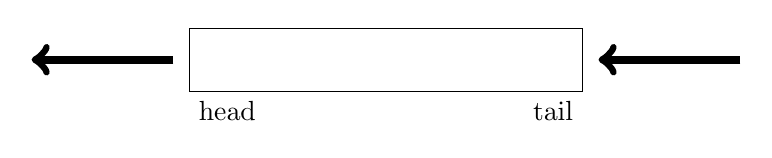
\begin{tikzpicture}

\draw (2.5, 0.4)
  node[draw, , , color=black,
       rounded corners=0cm, inner sep=0cm] {

\begin{minipage}[t][0.8cm]{5cm}
\mbox{}

\end{minipage}

};\draw[line width=0.1cm,black,->] (7,0.4) to  (5.2,0.4);
\draw[line width=0.1cm,black,->] (-0.2,0.4) to  (-2,0.4);

\node[anchor=north west] at (0,0)   {head};

\node[anchor=north east] at (5,0)   {tail};
\end{tikzpicture}

\end{center}



we will usually consider this instead:

\begin{center}
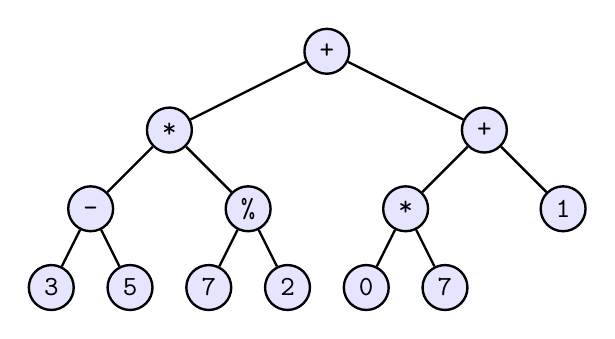
\begin{tikzpicture}

\fill[blue!10] (0.0, 0.0) circle (0.3);
\node [line width=0.03cm,black,minimum size=0.57cm,draw,circle] at (0.0,0.0)(+){};\draw (0.0, 0.0) node[color=black] {\texttt{+}};
\fill[blue!10] (-2.0, -1.0) circle (0.3);
\node [line width=0.03cm,black,minimum size=0.57cm,draw,circle] at (-2.0,-1.0)(*){};\draw (-2.0, -1.0) node[color=black] {\texttt{*}};
\fill[blue!10] (2.0, -1.0) circle (0.3);
\node [line width=0.03cm,black,minimum size=0.57cm,draw,circle] at (2.0,-1.0)(c){};\draw (2.0, -1.0) node[color=black] {\texttt{+}};
\fill[blue!10] (-3.0, -2.0) circle (0.3);
\node [line width=0.03cm,black,minimum size=0.57cm,draw,circle] at (-3.0,-2.0)(-){};\draw (-3.0, -2.0) node[color=black] {\texttt{-}};
\fill[blue!10] (-1.0, -2.0) circle (0.3);
\node [line width=0.03cm,black,minimum size=0.57cm,draw,circle] at (-1.0,-2.0)(e){};\draw (-1.0, -2.0) node[color=black] {\texttt{\%}};
\fill[blue!10] (1.0, -2.0) circle (0.3);
\node [line width=0.03cm,black,minimum size=0.57cm,draw,circle] at (1.0,-2.0)(f){};\draw (1.0, -2.0) node[color=black] {\texttt{*}};
\fill[blue!10] (3.0, -2.0) circle (0.3);
\node [line width=0.03cm,black,minimum size=0.57cm,draw,circle] at (3.0,-2.0)(1){};\draw (3.0, -2.0) node[color=black] {\texttt{1}};
\fill[blue!10] (-3.5, -3.0) circle (0.3);
\node [line width=0.03cm,black,minimum size=0.57cm,draw,circle] at (-3.5,-3.0)(3){};\draw (-3.5, -3.0) node[color=black] {\texttt{3}};
\fill[blue!10] (-2.5, -3.0) circle (0.3);
\node [line width=0.03cm,black,minimum size=0.57cm,draw,circle] at (-2.5,-3.0)(5){};\draw (-2.5, -3.0) node[color=black] {\texttt{5}};
\fill[blue!10] (-1.5, -3.0) circle (0.3);
\node [line width=0.03cm,black,minimum size=0.57cm,draw,circle] at (-1.5,-3.0)(z){};\draw (-1.5, -3.0) node[color=black] {\texttt{7}};
\fill[blue!10] (-0.5, -3.0) circle (0.3);
\node [line width=0.03cm,black,minimum size=0.57cm,draw,circle] at (-0.5,-3.0)(2){};\draw (-0.5, -3.0) node[color=black] {\texttt{2}};
\fill[blue!10] (0.5, -3.0) circle (0.3);
\node [line width=0.03cm,black,minimum size=0.57cm,draw,circle] at (0.5,-3.0)(0){};\draw (0.5, -3.0) node[color=black] {\texttt{0}};
\fill[blue!10] (1.5, -3.0) circle (0.3);
\node [line width=0.03cm,black,minimum size=0.57cm,draw,circle] at (1.5,-3.0)(7){};\draw (1.5, -3.0) node[color=black] {\texttt{7}};\draw[line width=0.03cm,black] (+) to  (*);
\draw[line width=0.03cm,black] (+) to  (c);
\draw[line width=0.03cm,black] (*) to  (-);
\draw[line width=0.03cm,black] (*) to  (e);
\draw[line width=0.03cm,black] (c) to  (f);
\draw[line width=0.03cm,black] (c) to  (1);
\draw[line width=0.03cm,black] (-) to  (3);
\draw[line width=0.03cm,black] (-) to  (5);
\draw[line width=0.03cm,black] (e) to  (z);
\draw[line width=0.03cm,black] (e) to  (2);
\draw[line width=0.03cm,black] (f) to  (0);
\draw[line width=0.03cm,black] (f) to  (7);
\end{tikzpicture}

\end{center}



This will ensure that when this heap is implemented
using an array, the values occupied are contiguous.

\begin{center}
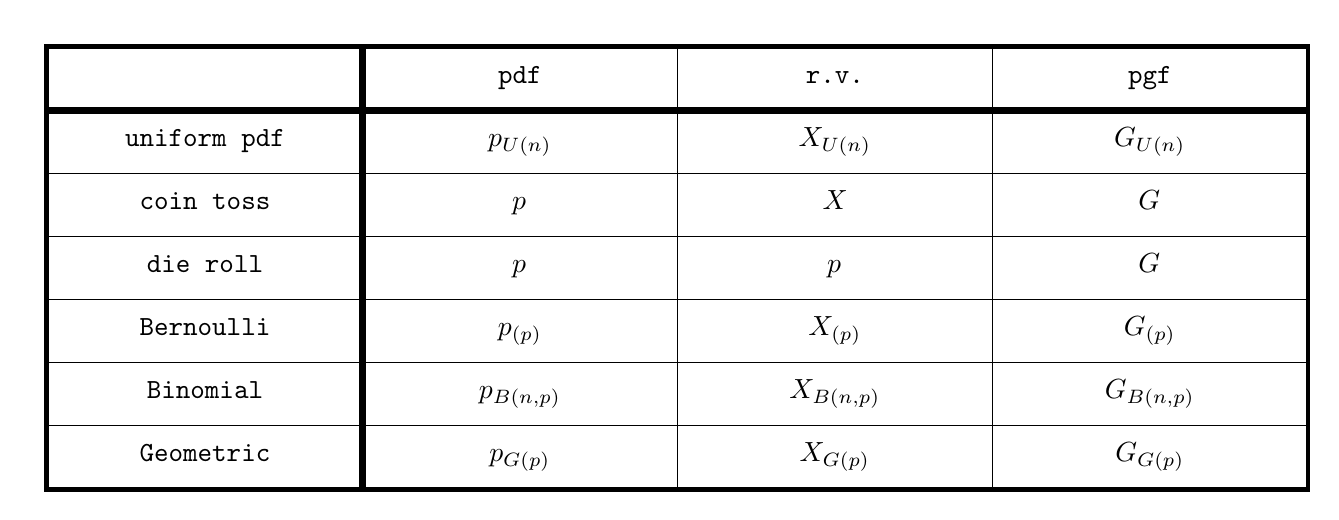
\begin{tikzpicture}

\draw (2.0, -0.4)
  node[draw, line width=0.02cm, , color=black,
       rounded corners=0cm, inner sep=0cm] {

\begin{minipage}[t][0.8cm]{4.0cm}
\mbox{}

\end{minipage}

};\draw (2.0, -0.4) node[color=black] {{\texttt{{\vphantom{pdfr.v.pgfuniform pdfcoin tossdie rollBernoulliBinomialGeometric$p_{U(n)}$$X_{U(n)}$$G_{U(n)}$$p_{\COIN}$$X_{\COIN}$$G_{\COIN}$$p_{\DIE}$$G_{\DIE}$$p_{\BERNOULLI(p)}$$X_{\BERNOULLI(p)}$$G_{\BERNOULLI(p)}$$p_{B(n,p)}$$X_{B(n,p)}$$G_{B(n,p)}$$p_{G(p)}$$X_{G(p)}$$G_{G(p)}$}}}}};\node[anchor=south] at (2.0,0.01) {};\node[anchor=east] at (-0.01,-0.4) {};
\draw (2.0, -0.4)
  node[draw, line width=0.06cm, , color=black,
       rounded corners=0cm, inner sep=0cm] {

\begin{minipage}[t][0.82cm]{4.02cm}
\mbox{}

\end{minipage}

};
\draw (6.0, -0.4)
  node[draw, line width=0.02cm, , color=black,
       rounded corners=0cm, inner sep=0cm] {

\begin{minipage}[t][0.8cm]{4.0cm}
\mbox{}

\end{minipage}

};\draw (6.0, -0.4) node[color=black] {{\texttt{{\vphantom{pdfr.v.pgfuniform pdfcoin tossdie rollBernoulliBinomialGeometric$p_{U(n)}$$X_{U(n)}$$G_{U(n)}$$p_{\COIN}$$X_{\COIN}$$G_{\COIN}$$p_{\DIE}$$G_{\DIE}$$p_{\BERNOULLI(p)}$$X_{\BERNOULLI(p)}$$G_{\BERNOULLI(p)}$$p_{B(n,p)}$$X_{B(n,p)}$$G_{B(n,p)}$$p_{G(p)}$$X_{G(p)}$$G_{G(p)}$}pdf}}}};
\draw (10.0, -0.4)
  node[draw, line width=0.02cm, , color=black,
       rounded corners=0cm, inner sep=0cm] {

\begin{minipage}[t][0.8cm]{4.0cm}
\mbox{}

\end{minipage}

};\draw (10.0, -0.4) node[color=black] {{\texttt{{\vphantom{pdfr.v.pgfuniform pdfcoin tossdie rollBernoulliBinomialGeometric$p_{U(n)}$$X_{U(n)}$$G_{U(n)}$$p_{\COIN}$$X_{\COIN}$$G_{\COIN}$$p_{\DIE}$$G_{\DIE}$$p_{\BERNOULLI(p)}$$X_{\BERNOULLI(p)}$$G_{\BERNOULLI(p)}$$p_{B(n,p)}$$X_{B(n,p)}$$G_{B(n,p)}$$p_{G(p)}$$X_{G(p)}$$G_{G(p)}$}r.v.}}}};
\draw (14.0, -0.4)
  node[draw, line width=0.02cm, , color=black,
       rounded corners=0cm, inner sep=0cm] {

\begin{minipage}[t][0.8cm]{4.0cm}
\mbox{}

\end{minipage}

};\draw (14.0, -0.4) node[color=black] {{\texttt{{\vphantom{pdfr.v.pgfuniform pdfcoin tossdie rollBernoulliBinomialGeometric$p_{U(n)}$$X_{U(n)}$$G_{U(n)}$$p_{\COIN}$$X_{\COIN}$$G_{\COIN}$$p_{\DIE}$$G_{\DIE}$$p_{\BERNOULLI(p)}$$X_{\BERNOULLI(p)}$$G_{\BERNOULLI(p)}$$p_{B(n,p)}$$X_{B(n,p)}$$G_{B(n,p)}$$p_{G(p)}$$X_{G(p)}$$G_{G(p)}$}pgf}}}};\node[anchor=south] at (6.0,0.01) {};\node[anchor=south] at (10.0,0.01) {};\node[anchor=south] at (14.0,0.01) {};\node[anchor=east] at (3.99,-0.4) {};
\draw (10.000000000000002, -0.4)
  node[draw, line width=0.06cm, , color=black,
       rounded corners=0cm, inner sep=0cm] {

\begin{minipage}[t][0.82cm]{12.02cm}
\mbox{}

\end{minipage}

};
\draw (2.0, -1.2000000000000002)
  node[draw, line width=0.02cm, , color=black,
       rounded corners=0cm, inner sep=0cm] {

\begin{minipage}[t][0.8cm]{4.0cm}
\mbox{}

\end{minipage}

};\draw (2.0, -1.2000000000000002) node[color=black] {{\texttt{{\vphantom{pdfr.v.pgfuniform pdfcoin tossdie rollBernoulliBinomialGeometric$p_{U(n)}$$X_{U(n)}$$G_{U(n)}$$p_{\COIN}$$X_{\COIN}$$G_{\COIN}$$p_{\DIE}$$G_{\DIE}$$p_{\BERNOULLI(p)}$$X_{\BERNOULLI(p)}$$G_{\BERNOULLI(p)}$$p_{B(n,p)}$$X_{B(n,p)}$$G_{B(n,p)}$$p_{G(p)}$$X_{G(p)}$$G_{G(p)}$}uniform pdf}}}};
\draw (2.0, -2.0)
  node[draw, line width=0.02cm, , color=black,
       rounded corners=0cm, inner sep=0cm] {

\begin{minipage}[t][0.8cm]{4.0cm}
\mbox{}

\end{minipage}

};\draw (2.0, -2.0) node[color=black] {{\texttt{{\vphantom{pdfr.v.pgfuniform pdfcoin tossdie rollBernoulliBinomialGeometric$p_{U(n)}$$X_{U(n)}$$G_{U(n)}$$p_{\COIN}$$X_{\COIN}$$G_{\COIN}$$p_{\DIE}$$G_{\DIE}$$p_{\BERNOULLI(p)}$$X_{\BERNOULLI(p)}$$G_{\BERNOULLI(p)}$$p_{B(n,p)}$$X_{B(n,p)}$$G_{B(n,p)}$$p_{G(p)}$$X_{G(p)}$$G_{G(p)}$}coin toss}}}};
\draw (2.0, -2.8000000000000003)
  node[draw, line width=0.02cm, , color=black,
       rounded corners=0cm, inner sep=0cm] {

\begin{minipage}[t][0.8cm]{4.0cm}
\mbox{}

\end{minipage}

};\draw (2.0, -2.8000000000000003) node[color=black] {{\texttt{{\vphantom{pdfr.v.pgfuniform pdfcoin tossdie rollBernoulliBinomialGeometric$p_{U(n)}$$X_{U(n)}$$G_{U(n)}$$p_{\COIN}$$X_{\COIN}$$G_{\COIN}$$p_{\DIE}$$G_{\DIE}$$p_{\BERNOULLI(p)}$$X_{\BERNOULLI(p)}$$G_{\BERNOULLI(p)}$$p_{B(n,p)}$$X_{B(n,p)}$$G_{B(n,p)}$$p_{G(p)}$$X_{G(p)}$$G_{G(p)}$}die roll}}}};
\draw (2.0, -3.6)
  node[draw, line width=0.02cm, , color=black,
       rounded corners=0cm, inner sep=0cm] {

\begin{minipage}[t][0.8cm]{4.0cm}
\mbox{}

\end{minipage}

};\draw (2.0, -3.6) node[color=black] {{\texttt{{\vphantom{pdfr.v.pgfuniform pdfcoin tossdie rollBernoulliBinomialGeometric$p_{U(n)}$$X_{U(n)}$$G_{U(n)}$$p_{\COIN}$$X_{\COIN}$$G_{\COIN}$$p_{\DIE}$$G_{\DIE}$$p_{\BERNOULLI(p)}$$X_{\BERNOULLI(p)}$$G_{\BERNOULLI(p)}$$p_{B(n,p)}$$X_{B(n,p)}$$G_{B(n,p)}$$p_{G(p)}$$X_{G(p)}$$G_{G(p)}$}Bernoulli}}}};
\draw (2.0, -4.4)
  node[draw, line width=0.02cm, , color=black,
       rounded corners=0cm, inner sep=0cm] {

\begin{minipage}[t][0.8cm]{4.0cm}
\mbox{}

\end{minipage}

};\draw (2.0, -4.4) node[color=black] {{\texttt{{\vphantom{pdfr.v.pgfuniform pdfcoin tossdie rollBernoulliBinomialGeometric$p_{U(n)}$$X_{U(n)}$$G_{U(n)}$$p_{\COIN}$$X_{\COIN}$$G_{\COIN}$$p_{\DIE}$$G_{\DIE}$$p_{\BERNOULLI(p)}$$X_{\BERNOULLI(p)}$$G_{\BERNOULLI(p)}$$p_{B(n,p)}$$X_{B(n,p)}$$G_{B(n,p)}$$p_{G(p)}$$X_{G(p)}$$G_{G(p)}$}Binomial}}}};
\draw (2.0, -5.199999999999999)
  node[draw, line width=0.02cm, , color=black,
       rounded corners=0cm, inner sep=0cm] {

\begin{minipage}[t][0.8cm]{4.0cm}
\mbox{}

\end{minipage}

};\draw (2.0, -5.199999999999999) node[color=black] {{\texttt{{\vphantom{pdfr.v.pgfuniform pdfcoin tossdie rollBernoulliBinomialGeometric$p_{U(n)}$$X_{U(n)}$$G_{U(n)}$$p_{\COIN}$$X_{\COIN}$$G_{\COIN}$$p_{\DIE}$$G_{\DIE}$$p_{\BERNOULLI(p)}$$X_{\BERNOULLI(p)}$$G_{\BERNOULLI(p)}$$p_{B(n,p)}$$X_{B(n,p)}$$G_{B(n,p)}$$p_{G(p)}$$X_{G(p)}$$G_{G(p)}$}Geometric}}}};\node[anchor=south] at (2.0,-0.79) {};\node[anchor=east] at (-0.01,-1.2000000000000002) {};\node[anchor=east] at (-0.01,-2.0000000000000004) {};\node[anchor=east] at (-0.01,-2.8000000000000003) {};\node[anchor=east] at (-0.01,-3.6) {};\node[anchor=east] at (-0.01,-4.4) {};\node[anchor=east] at (-0.01,-5.199999999999999) {};
\draw (2.0, -3.1999999999999997)
  node[draw, line width=0.06cm, , color=black,
       rounded corners=0cm, inner sep=0cm] {

\begin{minipage}[t][4.82cm]{4.02cm}
\mbox{}

\end{minipage}

};
\draw (6.0, -1.2000000000000002)
  node[draw, line width=0.02cm, , color=black,
       rounded corners=0cm, inner sep=0cm] {

\begin{minipage}[t][0.8cm]{4.0cm}
\mbox{}

\end{minipage}

};\draw (6.0, -1.2000000000000002) node[color=black] {{\texttt{{\vphantom{pdfr.v.pgfuniform pdfcoin tossdie rollBernoulliBinomialGeometric$p_{U(n)}$$X_{U(n)}$$G_{U(n)}$$p_{\COIN}$$X_{\COIN}$$G_{\COIN}$$p_{\DIE}$$G_{\DIE}$$p_{\BERNOULLI(p)}$$X_{\BERNOULLI(p)}$$G_{\BERNOULLI(p)}$$p_{B(n,p)}$$X_{B(n,p)}$$G_{B(n,p)}$$p_{G(p)}$$X_{G(p)}$$G_{G(p)}$}$p_{U(n)}$}}}};
\draw (10.0, -1.2000000000000002)
  node[draw, line width=0.02cm, , color=black,
       rounded corners=0cm, inner sep=0cm] {

\begin{minipage}[t][0.8cm]{4.0cm}
\mbox{}

\end{minipage}

};\draw (10.0, -1.2000000000000002) node[color=black] {{\texttt{{\vphantom{pdfr.v.pgfuniform pdfcoin tossdie rollBernoulliBinomialGeometric$p_{U(n)}$$X_{U(n)}$$G_{U(n)}$$p_{\COIN}$$X_{\COIN}$$G_{\COIN}$$p_{\DIE}$$G_{\DIE}$$p_{\BERNOULLI(p)}$$X_{\BERNOULLI(p)}$$G_{\BERNOULLI(p)}$$p_{B(n,p)}$$X_{B(n,p)}$$G_{B(n,p)}$$p_{G(p)}$$X_{G(p)}$$G_{G(p)}$}$X_{U(n)}$}}}};
\draw (14.0, -1.2000000000000002)
  node[draw, line width=0.02cm, , color=black,
       rounded corners=0cm, inner sep=0cm] {

\begin{minipage}[t][0.8cm]{4.0cm}
\mbox{}

\end{minipage}

};\draw (14.0, -1.2000000000000002) node[color=black] {{\texttt{{\vphantom{pdfr.v.pgfuniform pdfcoin tossdie rollBernoulliBinomialGeometric$p_{U(n)}$$X_{U(n)}$$G_{U(n)}$$p_{\COIN}$$X_{\COIN}$$G_{\COIN}$$p_{\DIE}$$G_{\DIE}$$p_{\BERNOULLI(p)}$$X_{\BERNOULLI(p)}$$G_{\BERNOULLI(p)}$$p_{B(n,p)}$$X_{B(n,p)}$$G_{B(n,p)}$$p_{G(p)}$$X_{G(p)}$$G_{G(p)}$}$G_{U(n)}$}}}};
\draw (6.0, -2.0)
  node[draw, line width=0.02cm, , color=black,
       rounded corners=0cm, inner sep=0cm] {

\begin{minipage}[t][0.8cm]{4.0cm}
\mbox{}

\end{minipage}

};\draw (6.0, -2.0) node[color=black] {{\texttt{{\vphantom{pdfr.v.pgfuniform pdfcoin tossdie rollBernoulliBinomialGeometric$p_{U(n)}$$X_{U(n)}$$G_{U(n)}$$p_{\COIN}$$X_{\COIN}$$G_{\COIN}$$p_{\DIE}$$G_{\DIE}$$p_{\BERNOULLI(p)}$$X_{\BERNOULLI(p)}$$G_{\BERNOULLI(p)}$$p_{B(n,p)}$$X_{B(n,p)}$$G_{B(n,p)}$$p_{G(p)}$$X_{G(p)}$$G_{G(p)}$}$p_{\COIN}$}}}};
\draw (10.0, -2.0)
  node[draw, line width=0.02cm, , color=black,
       rounded corners=0cm, inner sep=0cm] {

\begin{minipage}[t][0.8cm]{4.0cm}
\mbox{}

\end{minipage}

};\draw (10.0, -2.0) node[color=black] {{\texttt{{\vphantom{pdfr.v.pgfuniform pdfcoin tossdie rollBernoulliBinomialGeometric$p_{U(n)}$$X_{U(n)}$$G_{U(n)}$$p_{\COIN}$$X_{\COIN}$$G_{\COIN}$$p_{\DIE}$$G_{\DIE}$$p_{\BERNOULLI(p)}$$X_{\BERNOULLI(p)}$$G_{\BERNOULLI(p)}$$p_{B(n,p)}$$X_{B(n,p)}$$G_{B(n,p)}$$p_{G(p)}$$X_{G(p)}$$G_{G(p)}$}$X_{\COIN}$}}}};
\draw (14.0, -2.0)
  node[draw, line width=0.02cm, , color=black,
       rounded corners=0cm, inner sep=0cm] {

\begin{minipage}[t][0.8cm]{4.0cm}
\mbox{}

\end{minipage}

};\draw (14.0, -2.0) node[color=black] {{\texttt{{\vphantom{pdfr.v.pgfuniform pdfcoin tossdie rollBernoulliBinomialGeometric$p_{U(n)}$$X_{U(n)}$$G_{U(n)}$$p_{\COIN}$$X_{\COIN}$$G_{\COIN}$$p_{\DIE}$$G_{\DIE}$$p_{\BERNOULLI(p)}$$X_{\BERNOULLI(p)}$$G_{\BERNOULLI(p)}$$p_{B(n,p)}$$X_{B(n,p)}$$G_{B(n,p)}$$p_{G(p)}$$X_{G(p)}$$G_{G(p)}$}$G_{\COIN}$}}}};
\draw (6.0, -2.8000000000000003)
  node[draw, line width=0.02cm, , color=black,
       rounded corners=0cm, inner sep=0cm] {

\begin{minipage}[t][0.8cm]{4.0cm}
\mbox{}

\end{minipage}

};\draw (6.0, -2.8000000000000003) node[color=black] {{\texttt{{\vphantom{pdfr.v.pgfuniform pdfcoin tossdie rollBernoulliBinomialGeometric$p_{U(n)}$$X_{U(n)}$$G_{U(n)}$$p_{\COIN}$$X_{\COIN}$$G_{\COIN}$$p_{\DIE}$$G_{\DIE}$$p_{\BERNOULLI(p)}$$X_{\BERNOULLI(p)}$$G_{\BERNOULLI(p)}$$p_{B(n,p)}$$X_{B(n,p)}$$G_{B(n,p)}$$p_{G(p)}$$X_{G(p)}$$G_{G(p)}$}$p_{\DIE}$}}}};
\draw (10.0, -2.8000000000000003)
  node[draw, line width=0.02cm, , color=black,
       rounded corners=0cm, inner sep=0cm] {

\begin{minipage}[t][0.8cm]{4.0cm}
\mbox{}

\end{minipage}

};\draw (10.0, -2.8000000000000003) node[color=black] {{\texttt{{\vphantom{pdfr.v.pgfuniform pdfcoin tossdie rollBernoulliBinomialGeometric$p_{U(n)}$$X_{U(n)}$$G_{U(n)}$$p_{\COIN}$$X_{\COIN}$$G_{\COIN}$$p_{\DIE}$$G_{\DIE}$$p_{\BERNOULLI(p)}$$X_{\BERNOULLI(p)}$$G_{\BERNOULLI(p)}$$p_{B(n,p)}$$X_{B(n,p)}$$G_{B(n,p)}$$p_{G(p)}$$X_{G(p)}$$G_{G(p)}$}$p_{\DIE}$}}}};
\draw (14.0, -2.8000000000000003)
  node[draw, line width=0.02cm, , color=black,
       rounded corners=0cm, inner sep=0cm] {

\begin{minipage}[t][0.8cm]{4.0cm}
\mbox{}

\end{minipage}

};\draw (14.0, -2.8000000000000003) node[color=black] {{\texttt{{\vphantom{pdfr.v.pgfuniform pdfcoin tossdie rollBernoulliBinomialGeometric$p_{U(n)}$$X_{U(n)}$$G_{U(n)}$$p_{\COIN}$$X_{\COIN}$$G_{\COIN}$$p_{\DIE}$$G_{\DIE}$$p_{\BERNOULLI(p)}$$X_{\BERNOULLI(p)}$$G_{\BERNOULLI(p)}$$p_{B(n,p)}$$X_{B(n,p)}$$G_{B(n,p)}$$p_{G(p)}$$X_{G(p)}$$G_{G(p)}$}$G_{\DIE}$}}}};
\draw (6.0, -3.6)
  node[draw, line width=0.02cm, , color=black,
       rounded corners=0cm, inner sep=0cm] {

\begin{minipage}[t][0.8cm]{4.0cm}
\mbox{}

\end{minipage}

};\draw (6.0, -3.6) node[color=black] {{\texttt{{\vphantom{pdfr.v.pgfuniform pdfcoin tossdie rollBernoulliBinomialGeometric$p_{U(n)}$$X_{U(n)}$$G_{U(n)}$$p_{\COIN}$$X_{\COIN}$$G_{\COIN}$$p_{\DIE}$$G_{\DIE}$$p_{\BERNOULLI(p)}$$X_{\BERNOULLI(p)}$$G_{\BERNOULLI(p)}$$p_{B(n,p)}$$X_{B(n,p)}$$G_{B(n,p)}$$p_{G(p)}$$X_{G(p)}$$G_{G(p)}$}$p_{\BERNOULLI(p)}$}}}};
\draw (10.0, -3.6)
  node[draw, line width=0.02cm, , color=black,
       rounded corners=0cm, inner sep=0cm] {

\begin{minipage}[t][0.8cm]{4.0cm}
\mbox{}

\end{minipage}

};\draw (10.0, -3.6) node[color=black] {{\texttt{{\vphantom{pdfr.v.pgfuniform pdfcoin tossdie rollBernoulliBinomialGeometric$p_{U(n)}$$X_{U(n)}$$G_{U(n)}$$p_{\COIN}$$X_{\COIN}$$G_{\COIN}$$p_{\DIE}$$G_{\DIE}$$p_{\BERNOULLI(p)}$$X_{\BERNOULLI(p)}$$G_{\BERNOULLI(p)}$$p_{B(n,p)}$$X_{B(n,p)}$$G_{B(n,p)}$$p_{G(p)}$$X_{G(p)}$$G_{G(p)}$}$X_{\BERNOULLI(p)}$}}}};
\draw (14.0, -3.6)
  node[draw, line width=0.02cm, , color=black,
       rounded corners=0cm, inner sep=0cm] {

\begin{minipage}[t][0.8cm]{4.0cm}
\mbox{}

\end{minipage}

};\draw (14.0, -3.6) node[color=black] {{\texttt{{\vphantom{pdfr.v.pgfuniform pdfcoin tossdie rollBernoulliBinomialGeometric$p_{U(n)}$$X_{U(n)}$$G_{U(n)}$$p_{\COIN}$$X_{\COIN}$$G_{\COIN}$$p_{\DIE}$$G_{\DIE}$$p_{\BERNOULLI(p)}$$X_{\BERNOULLI(p)}$$G_{\BERNOULLI(p)}$$p_{B(n,p)}$$X_{B(n,p)}$$G_{B(n,p)}$$p_{G(p)}$$X_{G(p)}$$G_{G(p)}$}$G_{\BERNOULLI(p)}$}}}};
\draw (6.0, -4.4)
  node[draw, line width=0.02cm, , color=black,
       rounded corners=0cm, inner sep=0cm] {

\begin{minipage}[t][0.8cm]{4.0cm}
\mbox{}

\end{minipage}

};\draw (6.0, -4.4) node[color=black] {{\texttt{{\vphantom{pdfr.v.pgfuniform pdfcoin tossdie rollBernoulliBinomialGeometric$p_{U(n)}$$X_{U(n)}$$G_{U(n)}$$p_{\COIN}$$X_{\COIN}$$G_{\COIN}$$p_{\DIE}$$G_{\DIE}$$p_{\BERNOULLI(p)}$$X_{\BERNOULLI(p)}$$G_{\BERNOULLI(p)}$$p_{B(n,p)}$$X_{B(n,p)}$$G_{B(n,p)}$$p_{G(p)}$$X_{G(p)}$$G_{G(p)}$}$p_{B(n,p)}$}}}};
\draw (10.0, -4.4)
  node[draw, line width=0.02cm, , color=black,
       rounded corners=0cm, inner sep=0cm] {

\begin{minipage}[t][0.8cm]{4.0cm}
\mbox{}

\end{minipage}

};\draw (10.0, -4.4) node[color=black] {{\texttt{{\vphantom{pdfr.v.pgfuniform pdfcoin tossdie rollBernoulliBinomialGeometric$p_{U(n)}$$X_{U(n)}$$G_{U(n)}$$p_{\COIN}$$X_{\COIN}$$G_{\COIN}$$p_{\DIE}$$G_{\DIE}$$p_{\BERNOULLI(p)}$$X_{\BERNOULLI(p)}$$G_{\BERNOULLI(p)}$$p_{B(n,p)}$$X_{B(n,p)}$$G_{B(n,p)}$$p_{G(p)}$$X_{G(p)}$$G_{G(p)}$}$X_{B(n,p)}$}}}};
\draw (14.0, -4.4)
  node[draw, line width=0.02cm, , color=black,
       rounded corners=0cm, inner sep=0cm] {

\begin{minipage}[t][0.8cm]{4.0cm}
\mbox{}

\end{minipage}

};\draw (14.0, -4.4) node[color=black] {{\texttt{{\vphantom{pdfr.v.pgfuniform pdfcoin tossdie rollBernoulliBinomialGeometric$p_{U(n)}$$X_{U(n)}$$G_{U(n)}$$p_{\COIN}$$X_{\COIN}$$G_{\COIN}$$p_{\DIE}$$G_{\DIE}$$p_{\BERNOULLI(p)}$$X_{\BERNOULLI(p)}$$G_{\BERNOULLI(p)}$$p_{B(n,p)}$$X_{B(n,p)}$$G_{B(n,p)}$$p_{G(p)}$$X_{G(p)}$$G_{G(p)}$}$G_{B(n,p)}$}}}};
\draw (6.0, -5.199999999999999)
  node[draw, line width=0.02cm, , color=black,
       rounded corners=0cm, inner sep=0cm] {

\begin{minipage}[t][0.8cm]{4.0cm}
\mbox{}

\end{minipage}

};\draw (6.0, -5.199999999999999) node[color=black] {{\texttt{{\vphantom{pdfr.v.pgfuniform pdfcoin tossdie rollBernoulliBinomialGeometric$p_{U(n)}$$X_{U(n)}$$G_{U(n)}$$p_{\COIN}$$X_{\COIN}$$G_{\COIN}$$p_{\DIE}$$G_{\DIE}$$p_{\BERNOULLI(p)}$$X_{\BERNOULLI(p)}$$G_{\BERNOULLI(p)}$$p_{B(n,p)}$$X_{B(n,p)}$$G_{B(n,p)}$$p_{G(p)}$$X_{G(p)}$$G_{G(p)}$}$p_{G(p)}$}}}};
\draw (10.0, -5.199999999999999)
  node[draw, line width=0.02cm, , color=black,
       rounded corners=0cm, inner sep=0cm] {

\begin{minipage}[t][0.8cm]{4.0cm}
\mbox{}

\end{minipage}

};\draw (10.0, -5.199999999999999) node[color=black] {{\texttt{{\vphantom{pdfr.v.pgfuniform pdfcoin tossdie rollBernoulliBinomialGeometric$p_{U(n)}$$X_{U(n)}$$G_{U(n)}$$p_{\COIN}$$X_{\COIN}$$G_{\COIN}$$p_{\DIE}$$G_{\DIE}$$p_{\BERNOULLI(p)}$$X_{\BERNOULLI(p)}$$G_{\BERNOULLI(p)}$$p_{B(n,p)}$$X_{B(n,p)}$$G_{B(n,p)}$$p_{G(p)}$$X_{G(p)}$$G_{G(p)}$}$X_{G(p)}$}}}};
\draw (14.0, -5.199999999999999)
  node[draw, line width=0.02cm, , color=black,
       rounded corners=0cm, inner sep=0cm] {

\begin{minipage}[t][0.8cm]{4.0cm}
\mbox{}

\end{minipage}

};\draw (14.0, -5.199999999999999) node[color=black] {{\texttt{{\vphantom{pdfr.v.pgfuniform pdfcoin tossdie rollBernoulliBinomialGeometric$p_{U(n)}$$X_{U(n)}$$G_{U(n)}$$p_{\COIN}$$X_{\COIN}$$G_{\COIN}$$p_{\DIE}$$G_{\DIE}$$p_{\BERNOULLI(p)}$$X_{\BERNOULLI(p)}$$G_{\BERNOULLI(p)}$$p_{B(n,p)}$$X_{B(n,p)}$$G_{B(n,p)}$$p_{G(p)}$$X_{G(p)}$$G_{G(p)}$}$G_{G(p)}$}}}};\node[anchor=south] at (6.0,-0.79) {};\node[anchor=south] at (10.0,-0.79) {};\node[anchor=south] at (14.0,-0.79) {};\node[anchor=east] at (3.99,-1.2000000000000002) {};\node[anchor=east] at (3.99,-2.0000000000000004) {};\node[anchor=east] at (3.99,-2.8000000000000003) {};\node[anchor=east] at (3.99,-3.6) {};\node[anchor=east] at (3.99,-4.4) {};\node[anchor=east] at (3.99,-5.199999999999999) {};
\draw (10.000000000000002, -3.1999999999999997)
  node[draw, line width=0.06cm, , color=black,
       rounded corners=0cm, inner sep=0cm] {

\begin{minipage}[t][4.82cm]{12.02cm}
\mbox{}

\end{minipage}

};
\end{tikzpicture}

\end{center}



Cells which are not relevant are left blank.
Of course there are integer values there --
but we don't care about them.
Furthermore, this array would usually come with a
size or length variable (in the above example size would have value
\texttt{6}) which is the case if I use
\verb!std::vector!.
The size variable would tell me the index position of
the first available cell in the array

\begin{center}
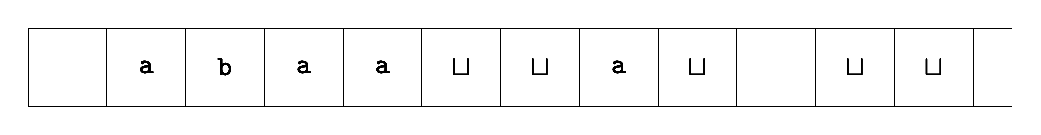
\begin{tikzpicture}

\draw (0.49999999999999994, 0.49999999999999994)
  node[draw, line width=0.01cm, , color=black,
       rounded corners=0cm, inner sep=0cm] {

\begin{minipage}[t][1.0cm]{1.0cm}
\mbox{}

\end{minipage}

};\draw (0.49999999999999994, 0.49999999999999994) node[color=black] {\texttt{\DOLLAR}};
\draw (1.5, 0.49999999999999994)
  node[draw, line width=0.01cm, , color=black,
       rounded corners=0cm, inner sep=0cm] {

\begin{minipage}[t][1.0cm]{1.0cm}
\mbox{}

\end{minipage}

};\draw (1.5, 0.49999999999999994) node[color=black] {\texttt{a}};
\draw (2.5, 0.49999999999999994)
  node[draw, line width=0.01cm, , color=black,
       rounded corners=0cm, inner sep=0cm] {

\begin{minipage}[t][1.0cm]{1.0cm}
\mbox{}

\end{minipage}

};\draw (2.5, 0.49999999999999994) node[color=black] {\texttt{b}};
\draw (3.5, 0.49999999999999994)
  node[draw, line width=0.01cm, , color=black,
       rounded corners=0cm, inner sep=0cm] {

\begin{minipage}[t][1.0cm]{1.0cm}
\mbox{}

\end{minipage}

};\draw (3.5, 0.49999999999999994) node[color=black] {\texttt{a}};
\draw (4.5, 0.49999999999999994)
  node[draw, line width=0.01cm, , color=black,
       rounded corners=0cm, inner sep=0cm] {

\begin{minipage}[t][1.0cm]{1.0cm}
\mbox{}

\end{minipage}

};\draw (4.5, 0.49999999999999994) node[color=black] {\texttt{a}};
\draw (5.5, 0.49999999999999994)
  node[draw, line width=0.01cm, , color=black,
       rounded corners=0cm, inner sep=0cm] {

\begin{minipage}[t][1.0cm]{1.0cm}
\mbox{}

\end{minipage}

};\draw (5.5, 0.49999999999999994) node[color=black] {\texttt{$\sqcup$}};
\draw (6.5, 0.49999999999999994)
  node[draw, line width=0.01cm, , color=black,
       rounded corners=0cm, inner sep=0cm] {

\begin{minipage}[t][1.0cm]{1.0cm}
\mbox{}

\end{minipage}

};\draw (6.5, 0.49999999999999994) node[color=black] {\texttt{$\sqcup$}};
\draw (7.5, 0.49999999999999994)
  node[draw, line width=0.01cm, , color=black,
       rounded corners=0cm, inner sep=0cm] {

\begin{minipage}[t][1.0cm]{1.0cm}
\mbox{}

\end{minipage}

};\draw (7.5, 0.49999999999999994) node[color=black] {\texttt{a}};
\draw (8.5, 0.49999999999999994)
  node[draw, line width=0.01cm, , color=black,
       rounded corners=0cm, inner sep=0cm] {

\begin{minipage}[t][1.0cm]{1.0cm}
\mbox{}

\end{minipage}

};\draw (8.5, 0.49999999999999994) node[color=black] {\texttt{$\sqcup$}};
\draw (9.5, 0.49999999999999994)
  node[draw, line width=0.01cm, , color=black,
       rounded corners=0cm, inner sep=0cm] {

\begin{minipage}[t][1.0cm]{1.0cm}
\mbox{}

\end{minipage}

};\draw (9.5, 0.49999999999999994) node[color=black] {\texttt{$\EOT$}};
\draw (10.5, 0.49999999999999994)
  node[draw, line width=0.01cm, , color=black,
       rounded corners=0cm, inner sep=0cm] {

\begin{minipage}[t][1.0cm]{1.0cm}
\mbox{}

\end{minipage}

};\draw (10.5, 0.49999999999999994) node[color=black] {\texttt{$\sqcup$}};
\draw (11.5, 0.49999999999999994)
  node[draw, line width=0.01cm, , color=black,
       rounded corners=0cm, inner sep=0cm] {

\begin{minipage}[t][1.0cm]{1.0cm}
\mbox{}

\end{minipage}

};\draw (11.5, 0.49999999999999994) node[color=black] {\texttt{$\sqcup$}};
\draw (0.49999999999999994, 0.49999999999999994)
  node[draw, line width=0.01cm, , color=black,
       rounded corners=0cm, inner sep=0cm] {

\begin{minipage}[t][1.0cm]{1.0cm}
\mbox{}

\end{minipage}

};\draw (0.49999999999999994, 0.49999999999999994) node[color=black] {\texttt{\DOLLAR}};
\draw (1.5, 0.49999999999999994)
  node[draw, line width=0.01cm, , color=black,
       rounded corners=0cm, inner sep=0cm] {

\begin{minipage}[t][1.0cm]{1.0cm}
\mbox{}

\end{minipage}

};\draw (1.5, 0.49999999999999994) node[color=black] {\texttt{a}};
\draw (2.5, 0.49999999999999994)
  node[draw, line width=0.01cm, , color=black,
       rounded corners=0cm, inner sep=0cm] {

\begin{minipage}[t][1.0cm]{1.0cm}
\mbox{}

\end{minipage}

};\draw (2.5, 0.49999999999999994) node[color=black] {\texttt{b}};
\draw (3.5, 0.49999999999999994)
  node[draw, line width=0.01cm, , color=black,
       rounded corners=0cm, inner sep=0cm] {

\begin{minipage}[t][1.0cm]{1.0cm}
\mbox{}

\end{minipage}

};\draw (3.5, 0.49999999999999994) node[color=black] {\texttt{a}};
\draw (4.5, 0.49999999999999994)
  node[draw, line width=0.01cm, , color=black,
       rounded corners=0cm, inner sep=0cm] {

\begin{minipage}[t][1.0cm]{1.0cm}
\mbox{}

\end{minipage}

};\draw (4.5, 0.49999999999999994) node[color=black] {\texttt{a}};
\draw (5.5, 0.49999999999999994)
  node[draw, line width=0.01cm, , color=black,
       rounded corners=0cm, inner sep=0cm] {

\begin{minipage}[t][1.0cm]{1.0cm}
\mbox{}

\end{minipage}

};\draw (5.5, 0.49999999999999994) node[color=black] {\texttt{$\sqcup$}};
\draw (6.5, 0.49999999999999994)
  node[draw, line width=0.01cm, , color=black,
       rounded corners=0cm, inner sep=0cm] {

\begin{minipage}[t][1.0cm]{1.0cm}
\mbox{}

\end{minipage}

};\draw (6.5, 0.49999999999999994) node[color=black] {\texttt{$\sqcup$}};
\draw (7.5, 0.49999999999999994)
  node[draw, line width=0.01cm, , color=black,
       rounded corners=0cm, inner sep=0cm] {

\begin{minipage}[t][1.0cm]{1.0cm}
\mbox{}

\end{minipage}

};\draw (7.5, 0.49999999999999994) node[color=black] {\texttt{a}};
\draw (8.5, 0.49999999999999994)
  node[draw, line width=0.01cm, , color=black,
       rounded corners=0cm, inner sep=0cm] {

\begin{minipage}[t][1.0cm]{1.0cm}
\mbox{}

\end{minipage}

};\draw (8.5, 0.49999999999999994) node[color=black] {\texttt{$\sqcup$}};
\draw (9.5, 0.49999999999999994)
  node[draw, line width=0.01cm, , color=black,
       rounded corners=0cm, inner sep=0cm] {

\begin{minipage}[t][1.0cm]{1.0cm}
\mbox{}

\end{minipage}

};\draw (9.5, 0.49999999999999994) node[color=black] {\texttt{$\EOT$}};
\draw (10.5, 0.49999999999999994)
  node[draw, line width=0.01cm, , color=black,
       rounded corners=0cm, inner sep=0cm] {

\begin{minipage}[t][1.0cm]{1.0cm}
\mbox{}

\end{minipage}

};\draw (10.5, 0.49999999999999994) node[color=black] {\texttt{$\sqcup$}};
\draw (11.5, 0.49999999999999994)
  node[draw, line width=0.01cm, , color=black,
       rounded corners=0cm, inner sep=0cm] {

\begin{minipage}[t][1.0cm]{1.0cm}
\mbox{}

\end{minipage}

};\draw (11.5, 0.49999999999999994) node[color=black] {\texttt{$\sqcup$}};
\draw (0.49999999999999994, 0.49999999999999994)
  node[draw, line width=0.01cm, , color=black,
       rounded corners=0cm, inner sep=0cm] {

\begin{minipage}[t][1.0cm]{1.0cm}
\mbox{}

\end{minipage}

};\draw (0.49999999999999994, 0.49999999999999994) node[color=black] {\texttt{\DOLLAR}};
\draw (1.5, 0.49999999999999994)
  node[draw, line width=0.01cm, , color=black,
       rounded corners=0cm, inner sep=0cm] {

\begin{minipage}[t][1.0cm]{1.0cm}
\mbox{}

\end{minipage}

};\draw (1.5, 0.49999999999999994) node[color=black] {\texttt{a}};
\draw (2.5, 0.49999999999999994)
  node[draw, line width=0.01cm, , color=black,
       rounded corners=0cm, inner sep=0cm] {

\begin{minipage}[t][1.0cm]{1.0cm}
\mbox{}

\end{minipage}

};\draw (2.5, 0.49999999999999994) node[color=black] {\texttt{b}};
\draw (3.5, 0.49999999999999994)
  node[draw, line width=0.01cm, , color=black,
       rounded corners=0cm, inner sep=0cm] {

\begin{minipage}[t][1.0cm]{1.0cm}
\mbox{}

\end{minipage}

};\draw (3.5, 0.49999999999999994) node[color=black] {\texttt{a}};
\draw (4.5, 0.49999999999999994)
  node[draw, line width=0.01cm, , color=black,
       rounded corners=0cm, inner sep=0cm] {

\begin{minipage}[t][1.0cm]{1.0cm}
\mbox{}

\end{minipage}

};\draw (4.5, 0.49999999999999994) node[color=black] {\texttt{a}};
\draw (5.5, 0.49999999999999994)
  node[draw, line width=0.01cm, , color=black,
       rounded corners=0cm, inner sep=0cm] {

\begin{minipage}[t][1.0cm]{1.0cm}
\mbox{}

\end{minipage}

};\draw (5.5, 0.49999999999999994) node[color=black] {\texttt{$\sqcup$}};
\draw (6.5, 0.49999999999999994)
  node[draw, line width=0.01cm, , color=black,
       rounded corners=0cm, inner sep=0cm] {

\begin{minipage}[t][1.0cm]{1.0cm}
\mbox{}

\end{minipage}

};\draw (6.5, 0.49999999999999994) node[color=black] {\texttt{$\sqcup$}};
\draw (7.5, 0.49999999999999994)
  node[draw, line width=0.01cm, , color=black,
       rounded corners=0cm, inner sep=0cm] {

\begin{minipage}[t][1.0cm]{1.0cm}
\mbox{}

\end{minipage}

};\draw (7.5, 0.49999999999999994) node[color=black] {\texttt{a}};
\draw (8.5, 0.49999999999999994)
  node[draw, line width=0.01cm, , color=black,
       rounded corners=0cm, inner sep=0cm] {

\begin{minipage}[t][1.0cm]{1.0cm}
\mbox{}

\end{minipage}

};\draw (8.5, 0.49999999999999994) node[color=black] {\texttt{$\sqcup$}};
\draw (9.5, 0.49999999999999994)
  node[draw, line width=0.01cm, , color=black,
       rounded corners=0cm, inner sep=0cm] {

\begin{minipage}[t][1.0cm]{1.0cm}
\mbox{}

\end{minipage}

};\draw (9.5, 0.49999999999999994) node[color=black] {\texttt{$\EOT$}};
\draw (10.5, 0.49999999999999994)
  node[draw, line width=0.01cm, , color=black,
       rounded corners=0cm, inner sep=0cm] {

\begin{minipage}[t][1.0cm]{1.0cm}
\mbox{}

\end{minipage}

};\draw (10.5, 0.49999999999999994) node[color=black] {\texttt{$\sqcup$}};
\draw (11.5, 0.49999999999999994)
  node[draw, line width=0.01cm, , color=black,
       rounded corners=0cm, inner sep=0cm] {

\begin{minipage}[t][1.0cm]{1.0cm}
\mbox{}

\end{minipage}

};\draw (11.5, 0.49999999999999994) node[color=black] {\texttt{$\sqcup$}};
\draw (0.49999999999999994, 0.49999999999999994)
  node[draw, line width=0.01cm, , color=black,
       rounded corners=0cm, inner sep=0cm] {

\begin{minipage}[t][1.0cm]{1.0cm}
\mbox{}

\end{minipage}

};\draw (0.49999999999999994, 0.49999999999999994) node[color=black] {\texttt{\DOLLAR}};
\draw (1.5, 0.49999999999999994)
  node[draw, line width=0.01cm, , color=black,
       rounded corners=0cm, inner sep=0cm] {

\begin{minipage}[t][1.0cm]{1.0cm}
\mbox{}

\end{minipage}

};\draw (1.5, 0.49999999999999994) node[color=black] {\texttt{a}};
\draw (2.5, 0.49999999999999994)
  node[draw, line width=0.01cm, , color=black,
       rounded corners=0cm, inner sep=0cm] {

\begin{minipage}[t][1.0cm]{1.0cm}
\mbox{}

\end{minipage}

};\draw (2.5, 0.49999999999999994) node[color=black] {\texttt{b}};
\draw (3.5, 0.49999999999999994)
  node[draw, line width=0.01cm, , color=black,
       rounded corners=0cm, inner sep=0cm] {

\begin{minipage}[t][1.0cm]{1.0cm}
\mbox{}

\end{minipage}

};\draw (3.5, 0.49999999999999994) node[color=black] {\texttt{a}};
\draw (4.5, 0.49999999999999994)
  node[draw, line width=0.01cm, , color=black,
       rounded corners=0cm, inner sep=0cm] {

\begin{minipage}[t][1.0cm]{1.0cm}
\mbox{}

\end{minipage}

};\draw (4.5, 0.49999999999999994) node[color=black] {\texttt{a}};
\draw (5.5, 0.49999999999999994)
  node[draw, line width=0.01cm, , color=black,
       rounded corners=0cm, inner sep=0cm] {

\begin{minipage}[t][1.0cm]{1.0cm}
\mbox{}

\end{minipage}

};\draw (5.5, 0.49999999999999994) node[color=black] {\texttt{$\sqcup$}};
\draw (6.5, 0.49999999999999994)
  node[draw, line width=0.01cm, , color=black,
       rounded corners=0cm, inner sep=0cm] {

\begin{minipage}[t][1.0cm]{1.0cm}
\mbox{}

\end{minipage}

};\draw (6.5, 0.49999999999999994) node[color=black] {\texttt{$\sqcup$}};
\draw (7.5, 0.49999999999999994)
  node[draw, line width=0.01cm, , color=black,
       rounded corners=0cm, inner sep=0cm] {

\begin{minipage}[t][1.0cm]{1.0cm}
\mbox{}

\end{minipage}

};\draw (7.5, 0.49999999999999994) node[color=black] {\texttt{a}};
\draw (8.5, 0.49999999999999994)
  node[draw, line width=0.01cm, , color=black,
       rounded corners=0cm, inner sep=0cm] {

\begin{minipage}[t][1.0cm]{1.0cm}
\mbox{}

\end{minipage}

};\draw (8.5, 0.49999999999999994) node[color=black] {\texttt{$\sqcup$}};
\draw (9.5, 0.49999999999999994)
  node[draw, line width=0.01cm, , color=black,
       rounded corners=0cm, inner sep=0cm] {

\begin{minipage}[t][1.0cm]{1.0cm}
\mbox{}

\end{minipage}

};\draw (9.5, 0.49999999999999994) node[color=black] {\texttt{$\EOT$}};
\draw (10.5, 0.49999999999999994)
  node[draw, line width=0.01cm, , color=black,
       rounded corners=0cm, inner sep=0cm] {

\begin{minipage}[t][1.0cm]{1.0cm}
\mbox{}

\end{minipage}

};\draw (10.5, 0.49999999999999994) node[color=black] {\texttt{$\sqcup$}};
\draw (11.5, 0.49999999999999994)
  node[draw, line width=0.01cm, , color=black,
       rounded corners=0cm, inner sep=0cm] {

\begin{minipage}[t][1.0cm]{1.0cm}
\mbox{}

\end{minipage}

};\draw (11.5, 0.49999999999999994) node[color=black] {\texttt{$\sqcup$}};
\draw (0.49999999999999994, 0.49999999999999994)
  node[draw, line width=0.01cm, , color=black,
       rounded corners=0cm, inner sep=0cm] {

\begin{minipage}[t][1.0cm]{1.0cm}
\mbox{}

\end{minipage}

};\draw (0.49999999999999994, 0.49999999999999994) node[color=black] {\texttt{\DOLLAR}};
\draw (1.5, 0.49999999999999994)
  node[draw, line width=0.01cm, , color=black,
       rounded corners=0cm, inner sep=0cm] {

\begin{minipage}[t][1.0cm]{1.0cm}
\mbox{}

\end{minipage}

};\draw (1.5, 0.49999999999999994) node[color=black] {\texttt{a}};
\draw (2.5, 0.49999999999999994)
  node[draw, line width=0.01cm, , color=black,
       rounded corners=0cm, inner sep=0cm] {

\begin{minipage}[t][1.0cm]{1.0cm}
\mbox{}

\end{minipage}

};\draw (2.5, 0.49999999999999994) node[color=black] {\texttt{b}};
\draw (3.5, 0.49999999999999994)
  node[draw, line width=0.01cm, , color=black,
       rounded corners=0cm, inner sep=0cm] {

\begin{minipage}[t][1.0cm]{1.0cm}
\mbox{}

\end{minipage}

};\draw (3.5, 0.49999999999999994) node[color=black] {\texttt{a}};
\draw (4.5, 0.49999999999999994)
  node[draw, line width=0.01cm, , color=black,
       rounded corners=0cm, inner sep=0cm] {

\begin{minipage}[t][1.0cm]{1.0cm}
\mbox{}

\end{minipage}

};\draw (4.5, 0.49999999999999994) node[color=black] {\texttt{a}};
\draw (5.5, 0.49999999999999994)
  node[draw, line width=0.01cm, , color=black,
       rounded corners=0cm, inner sep=0cm] {

\begin{minipage}[t][1.0cm]{1.0cm}
\mbox{}

\end{minipage}

};\draw (5.5, 0.49999999999999994) node[color=black] {\texttt{$\sqcup$}};
\draw (6.5, 0.49999999999999994)
  node[draw, line width=0.01cm, , color=black,
       rounded corners=0cm, inner sep=0cm] {

\begin{minipage}[t][1.0cm]{1.0cm}
\mbox{}

\end{minipage}

};\draw (6.5, 0.49999999999999994) node[color=black] {\texttt{$\sqcup$}};
\draw (7.5, 0.49999999999999994)
  node[draw, line width=0.01cm, , color=black,
       rounded corners=0cm, inner sep=0cm] {

\begin{minipage}[t][1.0cm]{1.0cm}
\mbox{}

\end{minipage}

};\draw (7.5, 0.49999999999999994) node[color=black] {\texttt{a}};
\draw (8.5, 0.49999999999999994)
  node[draw, line width=0.01cm, , color=black,
       rounded corners=0cm, inner sep=0cm] {

\begin{minipage}[t][1.0cm]{1.0cm}
\mbox{}

\end{minipage}

};\draw (8.5, 0.49999999999999994) node[color=black] {\texttt{$\sqcup$}};
\draw (9.5, 0.49999999999999994)
  node[draw, line width=0.01cm, , color=black,
       rounded corners=0cm, inner sep=0cm] {

\begin{minipage}[t][1.0cm]{1.0cm}
\mbox{}

\end{minipage}

};\draw (9.5, 0.49999999999999994) node[color=black] {\texttt{$\EOT$}};
\draw (10.5, 0.49999999999999994)
  node[draw, line width=0.01cm, , color=black,
       rounded corners=0cm, inner sep=0cm] {

\begin{minipage}[t][1.0cm]{1.0cm}
\mbox{}

\end{minipage}

};\draw (10.5, 0.49999999999999994) node[color=black] {\texttt{$\sqcup$}};
\draw (11.5, 0.49999999999999994)
  node[draw, line width=0.01cm, , color=black,
       rounded corners=0cm, inner sep=0cm] {

\begin{minipage}[t][1.0cm]{1.0cm}
\mbox{}

\end{minipage}

};\draw (11.5, 0.49999999999999994) node[color=black] {\texttt{$\sqcup$}};
\draw (0.49999999999999994, 0.49999999999999994)
  node[draw, line width=0.01cm, , color=black,
       rounded corners=0cm, inner sep=0cm] {

\begin{minipage}[t][1.0cm]{1.0cm}
\mbox{}

\end{minipage}

};\draw (0.49999999999999994, 0.49999999999999994) node[color=black] {\texttt{\DOLLAR}};
\draw (1.5, 0.49999999999999994)
  node[draw, line width=0.01cm, , color=black,
       rounded corners=0cm, inner sep=0cm] {

\begin{minipage}[t][1.0cm]{1.0cm}
\mbox{}

\end{minipage}

};\draw (1.5, 0.49999999999999994) node[color=black] {\texttt{a}};
\draw (2.5, 0.49999999999999994)
  node[draw, line width=0.01cm, , color=black,
       rounded corners=0cm, inner sep=0cm] {

\begin{minipage}[t][1.0cm]{1.0cm}
\mbox{}

\end{minipage}

};\draw (2.5, 0.49999999999999994) node[color=black] {\texttt{b}};
\draw (3.5, 0.49999999999999994)
  node[draw, line width=0.01cm, , color=black,
       rounded corners=0cm, inner sep=0cm] {

\begin{minipage}[t][1.0cm]{1.0cm}
\mbox{}

\end{minipage}

};\draw (3.5, 0.49999999999999994) node[color=black] {\texttt{a}};
\draw (4.5, 0.49999999999999994)
  node[draw, line width=0.01cm, , color=black,
       rounded corners=0cm, inner sep=0cm] {

\begin{minipage}[t][1.0cm]{1.0cm}
\mbox{}

\end{minipage}

};\draw (4.5, 0.49999999999999994) node[color=black] {\texttt{a}};
\draw (5.5, 0.49999999999999994)
  node[draw, line width=0.01cm, , color=black,
       rounded corners=0cm, inner sep=0cm] {

\begin{minipage}[t][1.0cm]{1.0cm}
\mbox{}

\end{minipage}

};\draw (5.5, 0.49999999999999994) node[color=black] {\texttt{$\sqcup$}};
\draw (6.5, 0.49999999999999994)
  node[draw, line width=0.01cm, , color=black,
       rounded corners=0cm, inner sep=0cm] {

\begin{minipage}[t][1.0cm]{1.0cm}
\mbox{}

\end{minipage}

};\draw (6.5, 0.49999999999999994) node[color=black] {\texttt{$\sqcup$}};
\draw (7.5, 0.49999999999999994)
  node[draw, line width=0.01cm, , color=black,
       rounded corners=0cm, inner sep=0cm] {

\begin{minipage}[t][1.0cm]{1.0cm}
\mbox{}

\end{minipage}

};\draw (7.5, 0.49999999999999994) node[color=black] {\texttt{a}};
\draw (8.5, 0.49999999999999994)
  node[draw, line width=0.01cm, , color=black,
       rounded corners=0cm, inner sep=0cm] {

\begin{minipage}[t][1.0cm]{1.0cm}
\mbox{}

\end{minipage}

};\draw (8.5, 0.49999999999999994) node[color=black] {\texttt{$\sqcup$}};
\draw (9.5, 0.49999999999999994)
  node[draw, line width=0.01cm, , color=black,
       rounded corners=0cm, inner sep=0cm] {

\begin{minipage}[t][1.0cm]{1.0cm}
\mbox{}

\end{minipage}

};\draw (9.5, 0.49999999999999994) node[color=black] {\texttt{$\EOT$}};
\draw (10.5, 0.49999999999999994)
  node[draw, line width=0.01cm, , color=black,
       rounded corners=0cm, inner sep=0cm] {

\begin{minipage}[t][1.0cm]{1.0cm}
\mbox{}

\end{minipage}

};\draw (10.5, 0.49999999999999994) node[color=black] {\texttt{$\sqcup$}};
\draw (11.5, 0.49999999999999994)
  node[draw, line width=0.01cm, , color=black,
       rounded corners=0cm, inner sep=0cm] {

\begin{minipage}[t][1.0cm]{1.0cm}
\mbox{}

\end{minipage}

};\draw (11.5, 0.49999999999999994) node[color=black] {\texttt{$\sqcup$}};
\draw (0.49999999999999994, 0.49999999999999994)
  node[draw, line width=0.01cm, , color=black,
       rounded corners=0cm, inner sep=0cm] {

\begin{minipage}[t][1.0cm]{1.0cm}
\mbox{}

\end{minipage}

};\draw (0.49999999999999994, 0.49999999999999994) node[color=black] {\texttt{\DOLLAR}};
\draw (1.5, 0.49999999999999994)
  node[draw, line width=0.01cm, , color=black,
       rounded corners=0cm, inner sep=0cm] {

\begin{minipage}[t][1.0cm]{1.0cm}
\mbox{}

\end{minipage}

};\draw (1.5, 0.49999999999999994) node[color=black] {\texttt{a}};
\draw (2.5, 0.49999999999999994)
  node[draw, line width=0.01cm, , color=black,
       rounded corners=0cm, inner sep=0cm] {

\begin{minipage}[t][1.0cm]{1.0cm}
\mbox{}

\end{minipage}

};\draw (2.5, 0.49999999999999994) node[color=black] {\texttt{b}};
\draw (3.5, 0.49999999999999994)
  node[draw, line width=0.01cm, , color=black,
       rounded corners=0cm, inner sep=0cm] {

\begin{minipage}[t][1.0cm]{1.0cm}
\mbox{}

\end{minipage}

};\draw (3.5, 0.49999999999999994) node[color=black] {\texttt{a}};
\draw (4.5, 0.49999999999999994)
  node[draw, line width=0.01cm, , color=black,
       rounded corners=0cm, inner sep=0cm] {

\begin{minipage}[t][1.0cm]{1.0cm}
\mbox{}

\end{minipage}

};\draw (4.5, 0.49999999999999994) node[color=black] {\texttt{a}};
\draw (5.5, 0.49999999999999994)
  node[draw, line width=0.01cm, , color=black,
       rounded corners=0cm, inner sep=0cm] {

\begin{minipage}[t][1.0cm]{1.0cm}
\mbox{}

\end{minipage}

};\draw (5.5, 0.49999999999999994) node[color=black] {\texttt{$\sqcup$}};
\draw (6.5, 0.49999999999999994)
  node[draw, line width=0.01cm, , color=black,
       rounded corners=0cm, inner sep=0cm] {

\begin{minipage}[t][1.0cm]{1.0cm}
\mbox{}

\end{minipage}

};\draw (6.5, 0.49999999999999994) node[color=black] {\texttt{$\sqcup$}};
\draw (7.5, 0.49999999999999994)
  node[draw, line width=0.01cm, , color=black,
       rounded corners=0cm, inner sep=0cm] {

\begin{minipage}[t][1.0cm]{1.0cm}
\mbox{}

\end{minipage}

};\draw (7.5, 0.49999999999999994) node[color=black] {\texttt{a}};
\draw (8.5, 0.49999999999999994)
  node[draw, line width=0.01cm, , color=black,
       rounded corners=0cm, inner sep=0cm] {

\begin{minipage}[t][1.0cm]{1.0cm}
\mbox{}

\end{minipage}

};\draw (8.5, 0.49999999999999994) node[color=black] {\texttt{$\sqcup$}};
\draw (9.5, 0.49999999999999994)
  node[draw, line width=0.01cm, , color=black,
       rounded corners=0cm, inner sep=0cm] {

\begin{minipage}[t][1.0cm]{1.0cm}
\mbox{}

\end{minipage}

};\draw (9.5, 0.49999999999999994) node[color=black] {\texttt{$\EOT$}};
\draw (10.5, 0.49999999999999994)
  node[draw, line width=0.01cm, , color=black,
       rounded corners=0cm, inner sep=0cm] {

\begin{minipage}[t][1.0cm]{1.0cm}
\mbox{}

\end{minipage}

};\draw (10.5, 0.49999999999999994) node[color=black] {\texttt{$\sqcup$}};
\draw (11.5, 0.49999999999999994)
  node[draw, line width=0.01cm, , color=black,
       rounded corners=0cm, inner sep=0cm] {

\begin{minipage}[t][1.0cm]{1.0cm}
\mbox{}

\end{minipage}

};\draw (11.5, 0.49999999999999994) node[color=black] {\texttt{$\sqcup$}};
\draw (0.49999999999999994, 0.49999999999999994)
  node[draw, line width=0.01cm, , color=black,
       rounded corners=0cm, inner sep=0cm] {

\begin{minipage}[t][1.0cm]{1.0cm}
\mbox{}

\end{minipage}

};\draw (0.49999999999999994, 0.49999999999999994) node[color=black] {\texttt{\DOLLAR}};
\draw (1.5, 0.49999999999999994)
  node[draw, line width=0.01cm, , color=black,
       rounded corners=0cm, inner sep=0cm] {

\begin{minipage}[t][1.0cm]{1.0cm}
\mbox{}

\end{minipage}

};\draw (1.5, 0.49999999999999994) node[color=black] {\texttt{a}};
\draw (2.5, 0.49999999999999994)
  node[draw, line width=0.01cm, , color=black,
       rounded corners=0cm, inner sep=0cm] {

\begin{minipage}[t][1.0cm]{1.0cm}
\mbox{}

\end{minipage}

};\draw (2.5, 0.49999999999999994) node[color=black] {\texttt{b}};
\draw (3.5, 0.49999999999999994)
  node[draw, line width=0.01cm, , color=black,
       rounded corners=0cm, inner sep=0cm] {

\begin{minipage}[t][1.0cm]{1.0cm}
\mbox{}

\end{minipage}

};\draw (3.5, 0.49999999999999994) node[color=black] {\texttt{a}};
\draw (4.5, 0.49999999999999994)
  node[draw, line width=0.01cm, , color=black,
       rounded corners=0cm, inner sep=0cm] {

\begin{minipage}[t][1.0cm]{1.0cm}
\mbox{}

\end{minipage}

};\draw (4.5, 0.49999999999999994) node[color=black] {\texttt{a}};
\draw (5.5, 0.49999999999999994)
  node[draw, line width=0.01cm, , color=black,
       rounded corners=0cm, inner sep=0cm] {

\begin{minipage}[t][1.0cm]{1.0cm}
\mbox{}

\end{minipage}

};\draw (5.5, 0.49999999999999994) node[color=black] {\texttt{$\sqcup$}};
\draw (6.5, 0.49999999999999994)
  node[draw, line width=0.01cm, , color=black,
       rounded corners=0cm, inner sep=0cm] {

\begin{minipage}[t][1.0cm]{1.0cm}
\mbox{}

\end{minipage}

};\draw (6.5, 0.49999999999999994) node[color=black] {\texttt{$\sqcup$}};
\draw (7.5, 0.49999999999999994)
  node[draw, line width=0.01cm, , color=black,
       rounded corners=0cm, inner sep=0cm] {

\begin{minipage}[t][1.0cm]{1.0cm}
\mbox{}

\end{minipage}

};\draw (7.5, 0.49999999999999994) node[color=black] {\texttt{a}};
\draw (8.5, 0.49999999999999994)
  node[draw, line width=0.01cm, , color=black,
       rounded corners=0cm, inner sep=0cm] {

\begin{minipage}[t][1.0cm]{1.0cm}
\mbox{}

\end{minipage}

};\draw (8.5, 0.49999999999999994) node[color=black] {\texttt{$\sqcup$}};
\draw (9.5, 0.49999999999999994)
  node[draw, line width=0.01cm, , color=black,
       rounded corners=0cm, inner sep=0cm] {

\begin{minipage}[t][1.0cm]{1.0cm}
\mbox{}

\end{minipage}

};\draw (9.5, 0.49999999999999994) node[color=black] {\texttt{$\EOT$}};
\draw (10.5, 0.49999999999999994)
  node[draw, line width=0.01cm, , color=black,
       rounded corners=0cm, inner sep=0cm] {

\begin{minipage}[t][1.0cm]{1.0cm}
\mbox{}

\end{minipage}

};\draw (10.5, 0.49999999999999994) node[color=black] {\texttt{$\sqcup$}};
\draw (11.5, 0.49999999999999994)
  node[draw, line width=0.01cm, , color=black,
       rounded corners=0cm, inner sep=0cm] {

\begin{minipage}[t][1.0cm]{1.0cm}
\mbox{}

\end{minipage}

};\draw (11.5, 0.49999999999999994) node[color=black] {\texttt{$\sqcup$}};
\draw (0.49999999999999994, 0.49999999999999994)
  node[draw, line width=0.01cm, , color=black,
       rounded corners=0cm, inner sep=0cm] {

\begin{minipage}[t][1.0cm]{1.0cm}
\mbox{}

\end{minipage}

};\draw (0.49999999999999994, 0.49999999999999994) node[color=black] {\texttt{\DOLLAR}};
\draw (1.5, 0.49999999999999994)
  node[draw, line width=0.01cm, , color=black,
       rounded corners=0cm, inner sep=0cm] {

\begin{minipage}[t][1.0cm]{1.0cm}
\mbox{}

\end{minipage}

};\draw (1.5, 0.49999999999999994) node[color=black] {\texttt{a}};
\draw (2.5, 0.49999999999999994)
  node[draw, line width=0.01cm, , color=black,
       rounded corners=0cm, inner sep=0cm] {

\begin{minipage}[t][1.0cm]{1.0cm}
\mbox{}

\end{minipage}

};\draw (2.5, 0.49999999999999994) node[color=black] {\texttt{b}};
\draw (3.5, 0.49999999999999994)
  node[draw, line width=0.01cm, , color=black,
       rounded corners=0cm, inner sep=0cm] {

\begin{minipage}[t][1.0cm]{1.0cm}
\mbox{}

\end{minipage}

};\draw (3.5, 0.49999999999999994) node[color=black] {\texttt{a}};
\draw (4.5, 0.49999999999999994)
  node[draw, line width=0.01cm, , color=black,
       rounded corners=0cm, inner sep=0cm] {

\begin{minipage}[t][1.0cm]{1.0cm}
\mbox{}

\end{minipage}

};\draw (4.5, 0.49999999999999994) node[color=black] {\texttt{a}};
\draw (5.5, 0.49999999999999994)
  node[draw, line width=0.01cm, , color=black,
       rounded corners=0cm, inner sep=0cm] {

\begin{minipage}[t][1.0cm]{1.0cm}
\mbox{}

\end{minipage}

};\draw (5.5, 0.49999999999999994) node[color=black] {\texttt{$\sqcup$}};
\draw (6.5, 0.49999999999999994)
  node[draw, line width=0.01cm, , color=black,
       rounded corners=0cm, inner sep=0cm] {

\begin{minipage}[t][1.0cm]{1.0cm}
\mbox{}

\end{minipage}

};\draw (6.5, 0.49999999999999994) node[color=black] {\texttt{$\sqcup$}};
\draw (7.5, 0.49999999999999994)
  node[draw, line width=0.01cm, , color=black,
       rounded corners=0cm, inner sep=0cm] {

\begin{minipage}[t][1.0cm]{1.0cm}
\mbox{}

\end{minipage}

};\draw (7.5, 0.49999999999999994) node[color=black] {\texttt{a}};
\draw (8.5, 0.49999999999999994)
  node[draw, line width=0.01cm, , color=black,
       rounded corners=0cm, inner sep=0cm] {

\begin{minipage}[t][1.0cm]{1.0cm}
\mbox{}

\end{minipage}

};\draw (8.5, 0.49999999999999994) node[color=black] {\texttt{$\sqcup$}};
\draw (9.5, 0.49999999999999994)
  node[draw, line width=0.01cm, , color=black,
       rounded corners=0cm, inner sep=0cm] {

\begin{minipage}[t][1.0cm]{1.0cm}
\mbox{}

\end{minipage}

};\draw (9.5, 0.49999999999999994) node[color=black] {\texttt{$\EOT$}};
\draw (10.5, 0.49999999999999994)
  node[draw, line width=0.01cm, , color=black,
       rounded corners=0cm, inner sep=0cm] {

\begin{minipage}[t][1.0cm]{1.0cm}
\mbox{}

\end{minipage}

};\draw (10.5, 0.49999999999999994) node[color=black] {\texttt{$\sqcup$}};
\draw (11.5, 0.49999999999999994)
  node[draw, line width=0.01cm, , color=black,
       rounded corners=0cm, inner sep=0cm] {

\begin{minipage}[t][1.0cm]{1.0cm}
\mbox{}

\end{minipage}

};\draw (11.5, 0.49999999999999994) node[color=black] {\texttt{$\sqcup$}};
\draw (0.49999999999999994, 0.49999999999999994)
  node[draw, line width=0.01cm, , color=black,
       rounded corners=0cm, inner sep=0cm] {

\begin{minipage}[t][1.0cm]{1.0cm}
\mbox{}

\end{minipage}

};\draw (0.49999999999999994, 0.49999999999999994) node[color=black] {\texttt{\DOLLAR}};
\draw (1.5, 0.49999999999999994)
  node[draw, line width=0.01cm, , color=black,
       rounded corners=0cm, inner sep=0cm] {

\begin{minipage}[t][1.0cm]{1.0cm}
\mbox{}

\end{minipage}

};\draw (1.5, 0.49999999999999994) node[color=black] {\texttt{a}};
\draw (2.5, 0.49999999999999994)
  node[draw, line width=0.01cm, , color=black,
       rounded corners=0cm, inner sep=0cm] {

\begin{minipage}[t][1.0cm]{1.0cm}
\mbox{}

\end{minipage}

};\draw (2.5, 0.49999999999999994) node[color=black] {\texttt{b}};
\draw (3.5, 0.49999999999999994)
  node[draw, line width=0.01cm, , color=black,
       rounded corners=0cm, inner sep=0cm] {

\begin{minipage}[t][1.0cm]{1.0cm}
\mbox{}

\end{minipage}

};\draw (3.5, 0.49999999999999994) node[color=black] {\texttt{a}};
\draw (4.5, 0.49999999999999994)
  node[draw, line width=0.01cm, , color=black,
       rounded corners=0cm, inner sep=0cm] {

\begin{minipage}[t][1.0cm]{1.0cm}
\mbox{}

\end{minipage}

};\draw (4.5, 0.49999999999999994) node[color=black] {\texttt{a}};
\draw (5.5, 0.49999999999999994)
  node[draw, line width=0.01cm, , color=black,
       rounded corners=0cm, inner sep=0cm] {

\begin{minipage}[t][1.0cm]{1.0cm}
\mbox{}

\end{minipage}

};\draw (5.5, 0.49999999999999994) node[color=black] {\texttt{$\sqcup$}};
\draw (6.5, 0.49999999999999994)
  node[draw, line width=0.01cm, , color=black,
       rounded corners=0cm, inner sep=0cm] {

\begin{minipage}[t][1.0cm]{1.0cm}
\mbox{}

\end{minipage}

};\draw (6.5, 0.49999999999999994) node[color=black] {\texttt{$\sqcup$}};
\draw (7.5, 0.49999999999999994)
  node[draw, line width=0.01cm, , color=black,
       rounded corners=0cm, inner sep=0cm] {

\begin{minipage}[t][1.0cm]{1.0cm}
\mbox{}

\end{minipage}

};\draw (7.5, 0.49999999999999994) node[color=black] {\texttt{a}};
\draw (8.5, 0.49999999999999994)
  node[draw, line width=0.01cm, , color=black,
       rounded corners=0cm, inner sep=0cm] {

\begin{minipage}[t][1.0cm]{1.0cm}
\mbox{}

\end{minipage}

};\draw (8.5, 0.49999999999999994) node[color=black] {\texttt{$\sqcup$}};
\draw (9.5, 0.49999999999999994)
  node[draw, line width=0.01cm, , color=black,
       rounded corners=0cm, inner sep=0cm] {

\begin{minipage}[t][1.0cm]{1.0cm}
\mbox{}

\end{minipage}

};\draw (9.5, 0.49999999999999994) node[color=black] {\texttt{$\EOT$}};
\draw (10.5, 0.49999999999999994)
  node[draw, line width=0.01cm, , color=black,
       rounded corners=0cm, inner sep=0cm] {

\begin{minipage}[t][1.0cm]{1.0cm}
\mbox{}

\end{minipage}

};\draw (10.5, 0.49999999999999994) node[color=black] {\texttt{$\sqcup$}};
\draw (11.5, 0.49999999999999994)
  node[draw, line width=0.01cm, , color=black,
       rounded corners=0cm, inner sep=0cm] {

\begin{minipage}[t][1.0cm]{1.0cm}
\mbox{}

\end{minipage}

};\draw (11.5, 0.49999999999999994) node[color=black] {\texttt{$\sqcup$}};
\draw (0.49999999999999994, 0.49999999999999994)
  node[draw, line width=0.01cm, , color=black,
       rounded corners=0cm, inner sep=0cm] {

\begin{minipage}[t][1.0cm]{1.0cm}
\mbox{}

\end{minipage}

};\draw (0.49999999999999994, 0.49999999999999994) node[color=black] {\texttt{\DOLLAR}};
\draw (1.5, 0.49999999999999994)
  node[draw, line width=0.01cm, , color=black,
       rounded corners=0cm, inner sep=0cm] {

\begin{minipage}[t][1.0cm]{1.0cm}
\mbox{}

\end{minipage}

};\draw (1.5, 0.49999999999999994) node[color=black] {\texttt{a}};
\draw (2.5, 0.49999999999999994)
  node[draw, line width=0.01cm, , color=black,
       rounded corners=0cm, inner sep=0cm] {

\begin{minipage}[t][1.0cm]{1.0cm}
\mbox{}

\end{minipage}

};\draw (2.5, 0.49999999999999994) node[color=black] {\texttt{b}};
\draw (3.5, 0.49999999999999994)
  node[draw, line width=0.01cm, , color=black,
       rounded corners=0cm, inner sep=0cm] {

\begin{minipage}[t][1.0cm]{1.0cm}
\mbox{}

\end{minipage}

};\draw (3.5, 0.49999999999999994) node[color=black] {\texttt{a}};
\draw (4.5, 0.49999999999999994)
  node[draw, line width=0.01cm, , color=black,
       rounded corners=0cm, inner sep=0cm] {

\begin{minipage}[t][1.0cm]{1.0cm}
\mbox{}

\end{minipage}

};\draw (4.5, 0.49999999999999994) node[color=black] {\texttt{a}};
\draw (5.5, 0.49999999999999994)
  node[draw, line width=0.01cm, , color=black,
       rounded corners=0cm, inner sep=0cm] {

\begin{minipage}[t][1.0cm]{1.0cm}
\mbox{}

\end{minipage}

};\draw (5.5, 0.49999999999999994) node[color=black] {\texttt{$\sqcup$}};
\draw (6.5, 0.49999999999999994)
  node[draw, line width=0.01cm, , color=black,
       rounded corners=0cm, inner sep=0cm] {

\begin{minipage}[t][1.0cm]{1.0cm}
\mbox{}

\end{minipage}

};\draw (6.5, 0.49999999999999994) node[color=black] {\texttt{$\sqcup$}};
\draw (7.5, 0.49999999999999994)
  node[draw, line width=0.01cm, , color=black,
       rounded corners=0cm, inner sep=0cm] {

\begin{minipage}[t][1.0cm]{1.0cm}
\mbox{}

\end{minipage}

};\draw (7.5, 0.49999999999999994) node[color=black] {\texttt{a}};
\draw (8.5, 0.49999999999999994)
  node[draw, line width=0.01cm, , color=black,
       rounded corners=0cm, inner sep=0cm] {

\begin{minipage}[t][1.0cm]{1.0cm}
\mbox{}

\end{minipage}

};\draw (8.5, 0.49999999999999994) node[color=black] {\texttt{$\sqcup$}};
\draw (9.5, 0.49999999999999994)
  node[draw, line width=0.01cm, , color=black,
       rounded corners=0cm, inner sep=0cm] {

\begin{minipage}[t][1.0cm]{1.0cm}
\mbox{}

\end{minipage}

};\draw (9.5, 0.49999999999999994) node[color=black] {\texttt{$\EOT$}};
\draw (10.5, 0.49999999999999994)
  node[draw, line width=0.01cm, , color=black,
       rounded corners=0cm, inner sep=0cm] {

\begin{minipage}[t][1.0cm]{1.0cm}
\mbox{}

\end{minipage}

};\draw (10.5, 0.49999999999999994) node[color=black] {\texttt{$\sqcup$}};
\draw (11.5, 0.49999999999999994)
  node[draw, line width=0.01cm, , color=black,
       rounded corners=0cm, inner sep=0cm] {

\begin{minipage}[t][1.0cm]{1.0cm}
\mbox{}

\end{minipage}

};\draw (11.5, 0.49999999999999994) node[color=black] {\texttt{$\sqcup$}};
\draw (0.49999999999999994, 0.49999999999999994)
  node[draw, line width=0.01cm, , color=black,
       rounded corners=0cm, inner sep=0cm] {

\begin{minipage}[t][1.0cm]{1.0cm}
\mbox{}

\end{minipage}

};\draw (0.49999999999999994, 0.49999999999999994) node[color=black] {\texttt{\DOLLAR}};
\draw (1.5, 0.49999999999999994)
  node[draw, line width=0.01cm, , color=black,
       rounded corners=0cm, inner sep=0cm] {

\begin{minipage}[t][1.0cm]{1.0cm}
\mbox{}

\end{minipage}

};\draw (1.5, 0.49999999999999994) node[color=black] {\texttt{a}};
\draw (2.5, 0.49999999999999994)
  node[draw, line width=0.01cm, , color=black,
       rounded corners=0cm, inner sep=0cm] {

\begin{minipage}[t][1.0cm]{1.0cm}
\mbox{}

\end{minipage}

};\draw (2.5, 0.49999999999999994) node[color=black] {\texttt{b}};
\draw (3.5, 0.49999999999999994)
  node[draw, line width=0.01cm, , color=black,
       rounded corners=0cm, inner sep=0cm] {

\begin{minipage}[t][1.0cm]{1.0cm}
\mbox{}

\end{minipage}

};\draw (3.5, 0.49999999999999994) node[color=black] {\texttt{a}};
\draw (4.5, 0.49999999999999994)
  node[draw, line width=0.01cm, , color=black,
       rounded corners=0cm, inner sep=0cm] {

\begin{minipage}[t][1.0cm]{1.0cm}
\mbox{}

\end{minipage}

};\draw (4.5, 0.49999999999999994) node[color=black] {\texttt{a}};
\draw (5.5, 0.49999999999999994)
  node[draw, line width=0.01cm, , color=black,
       rounded corners=0cm, inner sep=0cm] {

\begin{minipage}[t][1.0cm]{1.0cm}
\mbox{}

\end{minipage}

};\draw (5.5, 0.49999999999999994) node[color=black] {\texttt{$\sqcup$}};
\draw (6.5, 0.49999999999999994)
  node[draw, line width=0.01cm, , color=black,
       rounded corners=0cm, inner sep=0cm] {

\begin{minipage}[t][1.0cm]{1.0cm}
\mbox{}

\end{minipage}

};\draw (6.5, 0.49999999999999994) node[color=black] {\texttt{$\sqcup$}};
\draw (7.5, 0.49999999999999994)
  node[draw, line width=0.01cm, , color=black,
       rounded corners=0cm, inner sep=0cm] {

\begin{minipage}[t][1.0cm]{1.0cm}
\mbox{}

\end{minipage}

};\draw (7.5, 0.49999999999999994) node[color=black] {\texttt{a}};
\draw (8.5, 0.49999999999999994)
  node[draw, line width=0.01cm, , color=black,
       rounded corners=0cm, inner sep=0cm] {

\begin{minipage}[t][1.0cm]{1.0cm}
\mbox{}

\end{minipage}

};\draw (8.5, 0.49999999999999994) node[color=black] {\texttt{$\sqcup$}};
\draw (9.5, 0.49999999999999994)
  node[draw, line width=0.01cm, , color=black,
       rounded corners=0cm, inner sep=0cm] {

\begin{minipage}[t][1.0cm]{1.0cm}
\mbox{}

\end{minipage}

};\draw (9.5, 0.49999999999999994) node[color=black] {\texttt{$\EOT$}};
\draw (10.5, 0.49999999999999994)
  node[draw, line width=0.01cm, , color=black,
       rounded corners=0cm, inner sep=0cm] {

\begin{minipage}[t][1.0cm]{1.0cm}
\mbox{}

\end{minipage}

};\draw (10.5, 0.49999999999999994) node[color=black] {\texttt{$\sqcup$}};
\draw (11.5, 0.49999999999999994)
  node[draw, line width=0.01cm, , color=black,
       rounded corners=0cm, inner sep=0cm] {

\begin{minipage}[t][1.0cm]{1.0cm}
\mbox{}

\end{minipage}

};\draw (11.5, 0.49999999999999994) node[color=black] {\texttt{$\sqcup$}};\draw[line width=0.01cm,black] (12.0,1.0) to  (12.5,1.0);
\draw[line width=0.01cm,black] (12.0,0.0) to  (12.5,0.0);
\end{tikzpicture}

\end{center}



which would correspond nicely with the
next available node in the tree to keep the tree
in the \lq\lq heap shape'',
i.e., complete and unfilled nodes on a level
(if any) on the right:


\begin{center}
\begin{tikzpicture}[>=triangle 60,shorten >=0.5pt,node distance=2cm,auto,initial text=, double distance=2pt]
\node[state,initial] (A) at (  0,  0) {$q_0$};
\node[state] (B) at (  3,  0) {$q_1$};
\node[state,accepting] (C) at (  6,  0) {$q_2$};

\path[->]
(A) edge [loop above] node {$a$} ()
(A) edge [bend left=10,pos=0.5,above] node {$b$} (B)
(B) edge [bend left=10,pos=0.5] node {$a$} (A)
(B) edge [bend left=0,pos=0.5,above] node {$b$} (C)
(C) edge [loop above] node {$a,b$} ()

;
\end{tikzpicture}
\end{center}
    


From now on, I will assume that a max- or minheap
look like that,
i.e., is complete where the unfilled slots (if any)
are all on the same level
and all \lq\lq on the right''.

\newpage
\begin{ex}
How many maxheaps can you draw if the heap contains
the values 1, 2, 3, 4?
\qed
\end{ex}


\newpage
\begin{ex}
Suppose you have this array:
\[
5, 4, 3, 2, 1
\]
(index 0 is on the left).
Assume that this array represents a binary tree.
\begin{tightlist}
  \item Is this binary tree a maxheap?
  \item How many arrays with the above values represent a maxheap?
\end{tightlist}
\qed
\end{ex}

\newpage
\begin{ex}
  In the array representation of a complete tree of size $n$ where
  the leaves are all at the same depth and \lq\lq on the left",
  what are the index values of all the non-leaves
  and all the index values of all the leaves?
  How many non-leaves are there altogether?
  \qed
\end{ex}

\newpage%-*-latex-*-
\section{Heapify-up}

The following two operations are the basic tools for min- and maxheaps.

Look at this:

\begin{python}
from latextool_basic import *
from drawheap import *  
p = Plot()
edges={'10':['5','8'],
       '5':['2', '1'],
       '8':['3', '7'],
       '2':['0', '9'],
       }
drawheap(p, edges)
print(p)
\end{python}

It's almost a maxheap except for the \verb!9!.

What is the simplest way to make it a maxheap?
I compare \verb!9! with it's parent, i.e., \verb!2!.
Since this is a maxheap, something is wrong:
parents should be larger than children.
So I swap \verb!9! and \verb!2! to get:

\begin{python}
from latextool_basic import *
from drawheap import *  
p = Plot()
edges={'10':['5','8'],
       '5':['9', '1'],
       '8':['3', '7'],
       '9':['0', '2'],
       }
drawheap(p, edges)
print(p)
\end{python}

I then compare \verb!9! and \verb!5! and decide to swap again to get:

\begin{python}
from latextool_basic import *
from drawheap import *  
p = Plot()
edges={'10':['9','8'],
       '9':['5', '1'],
       '8':['3', '7'],
       '5':['0', '2'],
       }
drawheap(p, edges)
print(p)
\end{python}

Now it's a maxheap.
Basically, you continually swap the value in question with
its parent if the value is larger than the parent.

This is called
\defone{heapify-up}.
It's also called
\defone{bubble up} or
\defone{percolate up}.


In general, if \verb!x[0..n]! is an array
and I can talk about heapify-up on array \verb!x!
treating \verb!x! as a maxheap,
starting at index \verb!i! and going up
along its path to the root (i.e., index 0).

You can also talk about heapify-up on an array
treating it as a minheap,
starting at some index.

For a maxheap, to heapify-up at an index \verb!i!, you compare
\verb!x[i]! and \verb!x[parent(i)]!
and swap them if necessary, i.e. if \verb!x[i]! $>$ \verb!x[parent(i)]!
and you keep following that value up to the root.
If \verb!x[i]! $\leq$ \verb!x[parent(i)]!, you stop.
That's it.

\begin{Verbatim}[frame=single]
ALGORITHM: heapify-up (for maxheap)
INPUTS: x[0..n-1] -- array
        i         -- index of x

while 1:
    if parent(i) < 0: break
    if x[i] > x[parent(i)]:
        swap x[i], x[parent(i)]
        i = parent(i)
\end{Verbatim}

With a tiny of optimization:
\begin{Verbatim}[frame=single]
ALGORITHM: heapify-up (for maxheap)
INPUTS: x[0..n-1] -- array
        i         -- index of x

v = x[i]
while 1:
    p = parent(i)
    if p < 0: break
    if v <= x[p]:
        x[i] = v
        break
    else:
        x[i] = x[p]
        i = p
\end{Verbatim}

The same idea works for minheap.

\newpage%-*-latex-*-
\section{Heapify-down}

Heapify-down is the opposite of heapify-up:
you keep pushing a value \verb!v! down, swapping with the largest child
if that largest child is greater than \verb!v!. 
Here's an example.

Suppose I have this tree:

\begin{python}
from latextool_basic import *
from drawheap import *
p = Plot()
edges={'10':['0','8'],
       '0':['5','2'],
       '8':['4','6'],
       '5':['1','3']
       }
drawheap(p, edges, include_array=False)
print(p)
\end{python}

This is almost a maxheap except that \verb!0!
violates the maxheap property.
I perform heapify-down at \verb!0!, swapping with
the larger of the children, i.e., \verb!5!


\begin{python}
from latextool_basic import *
from drawheap import *
p = Plot()
edges={'10':['0','8'],
       '0':['5','2'],
       '8':['4','6'],
       '5':['1','3']
       }
drawheap(p, edges, include_array=False)
p += Line(names=['0', '5'], linewidth=0.03, linecolor='red',
          bend_right=60, endstyle='>', startstyle='>')       
print(p)
\end{python}

to get


\begin{python}
from latextool_basic import *
from drawheap import *
p = Plot()
edges={'10':['5','8'],
       '5':['0','2'],
       '8':['4','6'],
       '0':['1','3']
       }
drawheap(p, edges, include_array=False)
print(p)
\end{python}

I do it again, swapping \verb!0! with \verb!3! to get

\begin{python}
from latextool_basic import *
from drawheap import *
p = Plot()
edges={'10':['5','8'],
       '5':['3','2'],
       '8':['4','6'],
       '3':['1','0']
       }
drawheap(p, edges, include_array=False)
print(p)
\end{python}

In this case, I stop at a leaf.
In general, it's possible that the heapify-down stops before
arriving at a leaf.

Note that I can heapify-down at any value even if
the tree has multiple spots that violate the
maxheap property.

\begin{Verbatim}[frame=single]
ALGORITHM: heapify-down (for maxheap)
INPUTS: x[0..n-1] -- array
        i         -- index of x

while i < n and x[i] has a child larger than x[i]:
    swap x[i] with the largest child, say x[j]
    set i to j
x[i] = val
\end{Verbatim}

In more details:

\begin{Verbatim}[frame=single]
ALGORITHM: heapify-down (for maxheap)
INPUTS: x[0..n-1] -- array
        i         -- index of x

v = x[i]
while 1:

    # Set j to index of the larger of the left and right
    # child of v. If there is no left and right child,
    # j is set to -1.
    l = left(i)
    r = right(i)
    if l == -1:
        # left child does no exist
        # (therefore right child does not exist)
        j = -1
    else:
        # left child exists
        if r == -1:
            # right child does not exists
            j = l
        else:
            # right child exists
            if x[l] > x[r]:
                j = l
            else:
                j = r    

    if j != -1 and x[j] > v:
        # v heapify-down                
        x[i] = x[j]
        i = j
    else:
        # v arrives at final index
        x[i] = v
        break
\end{Verbatim}

[REDUNDANT PARAGRAPH]
You can heapify-up or heapify-down at any index position.
There are times when heapifying-up or heapifying-down depends on the
value at the given index.
Let's call the function \verb!heapify!.
In such cases, if it's possible to heapify-up, then \verb!heapify! will
heapify-up and if it's possible to heapify-down, then \verb!heapify!
will heapify-down.

[What if there's a value that can heapify up and can heapify down?]


\begin{ex}
  In terms if actual real time, which cost more, one step of
  heapify-up or one step of heapify-down?
  \qed
\end{ex}

\newpage%-*-latex-*-
\section{Insert}

Look at this maxheap again:

\begin{python}
from latextool_basic import *
p = Plot()
edges={'10':['5','7'],
       '5':['2', '1'],
       '7':['0'],
       }
drawheap(p, edges, include_array=False)
print(p)
\end{python}

Suppose I want to insert a \verb!3! into the above tree.
To maintain the shape of a heap, I have to do it here:

\begin{python}
from latextool_basic import *
p = Plot()
edges={'10':['5','7'],
       '5':['2', '1'],
       '7':['0', '3'],
     }
#BinTree.node_hsep=0.2
drawheap(p, edges, include_array=False)
print(p)
\end{python}


(Don't forget that heaps are implemented with arrays
and therefore I can find the available slots in the array
right away with the length variable of the array.)
In this case the tree becomes perfect.
It's also a maxheap.

But what if I want to add \verb!8! into the tree instead?
I can again put it at the same spot:

\begin{python}
from latextool_basic import *
p = Plot()
edges={'10':['5','7'],
       '5':['2', '1'],
       '7':['0', '8'],
     }
#BinTree.node_hsep=0.2
drawheap(p, edges, include_array=False)
print(p)
\end{python}

Of course this is not a maxheap any more.
What do I do?
I heapify-up.
I look at \verb!8!
and swap it with its parent if \verb!8! is larger than
its parent.
In this case, the parent is \verb!7!, so I swap them:

\begin{python}
from latextool_basic import *
p = Plot()
edges={'10':['5','7'],
       '5':['2', '1'],
       '7':['0', '8'],
     }
#BinTree.node_hsep=0.2
p += Line(names=['7', '8'], linecolor='red', bend_left=90,
          linewidth=0.03, endstyle='>', startstyle='>')
drawheap(p, edges, include_array=False)
print(p)
\end{python}

to get

\begin{python}
from latextool_basic import *
p = Plot()
edges={'10':['5','8'],
       '5':['2', '1'],
       '8':['0', '7'],
     }
#BinTree.node_hsep=0.2
drawheap(p, edges, include_array=False)
print(p)
\end{python}

Now it's a maxheap again.
In general recall that heapify-up might involve
more than one swap.

In terms of the array implementation of the above heap, basically
this:

\begin{python}
from latextool_basic import *
p = Plot()
p += Array2d(0, 0, width=0.6, height=0.6, 
             xs=[['10','5','7','2','1','0','8']])
print(p)
\end{python}

becomes this:

\begin{python}
from latextool_basic import *
p = Plot()
p += Array2d(0, 0, width=0.6, height=0.6, 
             xs=[['10','5','8','2','1','0','7']])
print(p)
\end{python}

(Don't forget that technically speaking, there should also be a
length variable.)

Suppose I do this again: I add a \verb!9!.
It must go here:

\begin{python}
from latextool_basic import *
p = Plot()
edges={'10':['5','8'],
       '5':['2', '1'],
       '8':['0', '7'],
       '2':['9'],
     }
#BinTree.node_hsep=0.2
drawheap(p, edges, include_array=False)
print(p)
\end{python}

(Draw the array implementation for the above.)
I swap \verb!9! and \verb!2! to get this:

\begin{python}
from latextool_basic import *
p = Plot()
edges={'10':['5','8'],
       '5':['9', '1'],
       '8':['0', '7'],
       '9':['2'],
     }
#BinTree.node_hsep=0.2
drawheap(p, edges, include_array=False)
print(p)
\end{python}

and then swap \verb!9! and \verb!5! to get

\begin{python}
from latextool_basic import *
p = Plot()
edges={'10':['9','8'],
       '9':['5', '1'],
       '8':['0', '7'],
       '5':['2'],
     }
#BinTree.node_hsep=0.2
drawheap(p, edges, include_array=False)
print(p)
\end{python}

(Draw the arrays for the above so that you see how the array changes.)

This works even when you swap all the way to the root.
Say I add a \verb!20!.
It must go here:

\begin{python}
from latextool_basic import *
p = Plot()
edges={'10':['9','8'],
       '9':['5', '1'],
       '8':['0', '7'],
       '5':['2', '20'],
     }
drawheap(p, edges, include_array=False)
print(p)
\end{python}

After 3 swaps I get:

\begin{python}
from latextool_basic import *
p = Plot()
edges={'20':['10','8'],
       '10':['9', '1'],
       '8':['0', '7'],
       '9':['2', '5'],
     }
#BinTree.node_hsep=0.2
drawheap(p, edges, include_array=False)
print(p)
\end{python}

and I get a maxheap again.

This process is called
\defterm{heapify-up}\tinysidebar{bubble-up \\ heapify-up \\ percolate up}
or
\defterm{bubble-up}
or
\defterm{percolate-up}.

\begin{ex}
Draw the maxheap after each
of the above swaps and draw the corresponding array.
\qed
\end{ex}
  
Now if you think about it,
if you have the following
\begin{python}
from latextool_basic import *
print(r"""
\begin{center}
%s
\end{center}
""" % graph(yscale=1, xscale=1,
layout="""
   A 
     C
    F G
   H I
""",
minimum_size='8mm',
edges='A-C,C-G,C-F,F-H,F-I',
A=r'shape=None,label=\texttt{}',
B=r'label=\texttt{5}',
C=r'label=$\alpha$',
D=r'label=\texttt{2}',
E=r'label=\texttt{1}',
F=r'label=$\beta$',
G=r'shape=tree,label=$T_3$',
H=r'shape=tree,label=$T_1$',
I=r'shape=tree,label=$T_2$',
))
\end{python}

where 
\begin{tightlist}
\li the subtree at $\beta$ is a maxheap,
\li the subtree at $\alpha$ is also a maxheap if we ignore the 
its left subtree, 
\li and $\beta > \alpha$, 
\end{tightlist}
then
on swapping $\alpha$ and $\beta$:
\begin{python}
from latextool_basic import *
print(r"""
\begin{center}
%s
\end{center}
""" % graph(yscale=1, xscale=1,
layout="""
   A 
     C
    F G
   H I
""",
minimum_size='8mm',
edges='A-C,C-G,C-F,F-H,F-I',
A=r'shape=None,label=\texttt{}',
B=r'label=\texttt{5}',
C=r'label=$\beta$',
D=r'label=\texttt{2}',
E=r'label=\texttt{1}',
F=r'label=$\alpha$',
G=r'shape=tree,label=$T_3$',
H=r'shape=tree,label=$T_1$',
I=r'shape=tree,label=$T_2$',
))
\end{python}

we have a maxheap at $\beta$.

\begin{console}[commandchars=\\\{\}]
ALGORITHM: heap_insert (for maxheap)
INPUT: x - an array representing a heap
       n - length of heap (pass by reference)
       key - value to be inserted

insert node with key as a leaf in the right place, i.e.,
x[n] = key
n = n + 1 (note that now the key is at index n - 1)
heapify_up(x, n - 1)
\end{console}

The corresponding algorithm for minheap is similar.

Note that the runtime is
\[
O(\log n)
\]
Why?
Because the heapify-up basically \lq\lq bubble up''
the inserted key value from the point of insert (at leaf level)
up to the root,
possibly stopping before reaching the root.
But in the worse case, this means that
worse runtime depends on the height which is $O(\log n)$
since the tree is complete.



%One really important thing to note is this:
%this works no matter where you put the new node with the new value:
%any leaf position will work.


\newpage
\begin{ex}
  Starting with this maxheap:

\begin{python}
from latextool_basic import *
p = Plot()
edges={'20':['10','8'],
       '10':['9', '1'],
       '8':['0', '7'],
       '9':['2', '5'],
     }
#BinTree.node_hsep=0.2
drawheap(p, edges, include_array=False)
print(p)
\end{python}


Do the following assuming that the array implementation
of the above heap is an array of size 20.
\begin{tightlist}
\item Draw the array implementation of the above maxheap.
\item Insert \texttt{5}. Draw the maxheap after the insert
and after each necessary swap (technically, until all the swaps are done
the tree is not a max heap). Draw the array implementation
after each swap.
\item Do the same with \texttt{15}.
\item Do the same with \texttt{11}.
\item Do the same with \texttt{22}.
\end{tightlist}
\qed
\end{ex}


\newpage
\begin{ex}
Starting with an empty \textit{min} heap.
Do the following, drawing the heap and the array implementation.
\begin{tightlist}
  \item Insert \texttt{10}.
  \item Insert \texttt{15}.
  \item Insert \texttt{5}.
  \item Insert \texttt{2}.
  \item Insert \texttt{8}.
  \item Insert \texttt{0}.
  \item Insert \texttt{5}.
\end{tightlist}
(First, you want to study the operations for maxheap very carefully.
Then, you translate the operations to the case of minheap.)
\qed
\end{ex}


\newpage%-*-latex-*-
\sectionthree{Delete and extract-root}
\begin{python0}
  from solutions import *; clear()
\end{python0}

Suppose I want to delete
\texttt{8}
from this maxheap:

\begin{center}
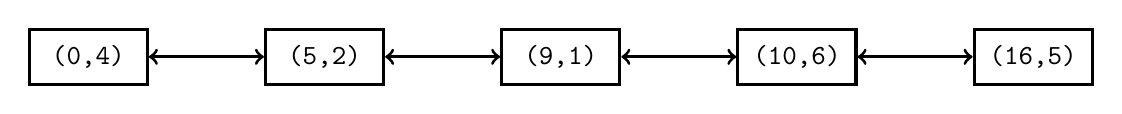
\begin{tikzpicture}

\draw (0.75, 0.35)
  node[draw, line width=0.04cm, , color=black,
       rounded corners=0cm, inner sep=0cm] {

\begin{minipage}[t][0.7cm]{1.5cm}
\mbox{}

\end{minipage}

};\draw (0.75, 0.35) node[color=black] {{\texttt{(0,4)}}};
\draw (3.75, 0.35)
  node[draw, line width=0.04cm, , color=black,
       rounded corners=0cm, inner sep=0cm] {

\begin{minipage}[t][0.7cm]{1.5cm}
\mbox{}

\end{minipage}

};\draw (3.75, 0.35) node[color=black] {{\texttt{(5,2)}}};
\draw (6.75, 0.35)
  node[draw, line width=0.04cm, , color=black,
       rounded corners=0cm, inner sep=0cm] {

\begin{minipage}[t][0.7cm]{1.5cm}
\mbox{}

\end{minipage}

};\draw (6.75, 0.35) node[color=black] {{\texttt{(9,1)}}};
\draw (9.75, 0.35)
  node[draw, line width=0.04cm, , color=black,
       rounded corners=0cm, inner sep=0cm] {

\begin{minipage}[t][0.7cm]{1.5cm}
\mbox{}

\end{minipage}

};\draw (9.75, 0.35) node[color=black] {{\texttt{(10,6)}}};
\draw (12.75, 0.35)
  node[draw, line width=0.04cm, , color=black,
       rounded corners=0cm, inner sep=0cm] {

\begin{minipage}[t][0.7cm]{1.5cm}
\mbox{}

\end{minipage}

};\draw (12.75, 0.35) node[color=black] {{\texttt{(16,5)}}};\draw[line width=0.04cm,black,<->] (1.52,0.35) to  (2.98,0.35);
\draw[line width=0.04cm,black,<->] (4.52,0.35) to  (5.98,0.35);
\draw[line width=0.04cm,black,<->] (7.52,0.35) to  (8.98,0.35);
\draw[line width=0.04cm,black,<->] (10.52,0.35) to  (11.98,0.35);
\end{tikzpicture}

\end{center}



In other words I want to delete the value at index 2
in the array implementation of the above heap.

I'll do it this way:
I look for the rightmost node of the last level --
this corresponds to the last value in the array implementation.
In the above case, that's the value \texttt{5}.
I then overwrite \texttt{8} with \texttt{5}:

\begin{center}
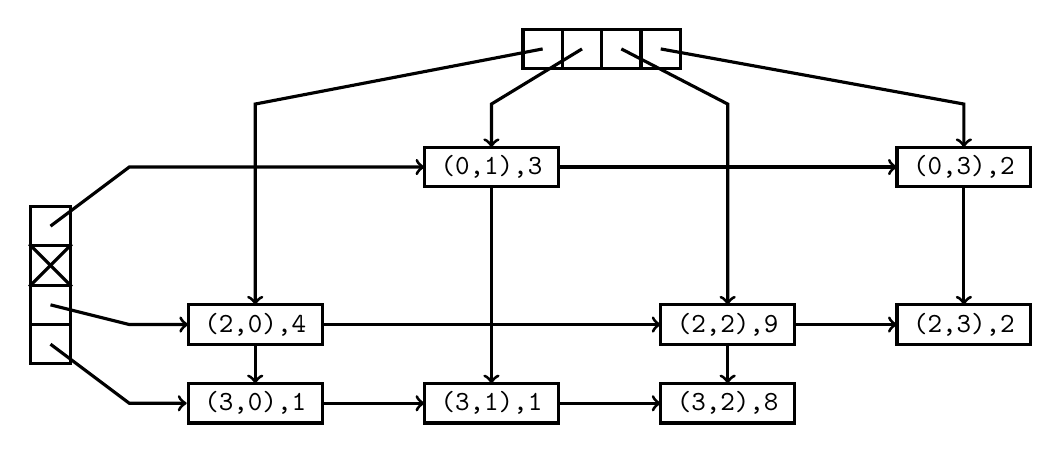
\begin{tikzpicture}

\draw (3.8499999999999996, 3.25)
  node[draw, line width=0.04cm, , color=black,
       rounded corners=0cm, inner sep=0cm] {

\begin{minipage}[t][0.5cm]{1.7cm}
\mbox{}

\end{minipage}

};\draw (3.8499999999999996, 3.25) node[color=black] {{\texttt{(0,1),3}}};
\draw (9.85, 3.25)
  node[draw, line width=0.04cm, , color=black,
       rounded corners=0cm, inner sep=0cm] {

\begin{minipage}[t][0.5cm]{1.7cm}
\mbox{}

\end{minipage}

};\draw (9.85, 3.25) node[color=black] {{\texttt{(0,3),2}}};
\draw (0.85, 1.25)
  node[draw, line width=0.04cm, , color=black,
       rounded corners=0cm, inner sep=0cm] {

\begin{minipage}[t][0.5cm]{1.7cm}
\mbox{}

\end{minipage}

};\draw (0.85, 1.25) node[color=black] {{\texttt{(2,0),4}}};
\draw (6.85, 1.25)
  node[draw, line width=0.04cm, , color=black,
       rounded corners=0cm, inner sep=0cm] {

\begin{minipage}[t][0.5cm]{1.7cm}
\mbox{}

\end{minipage}

};\draw (6.85, 1.25) node[color=black] {{\texttt{(2,2),9}}};
\draw (9.85, 1.25)
  node[draw, line width=0.04cm, , color=black,
       rounded corners=0cm, inner sep=0cm] {

\begin{minipage}[t][0.5cm]{1.7cm}
\mbox{}

\end{minipage}

};\draw (9.85, 1.25) node[color=black] {{\texttt{(2,3),2}}};
\draw (0.85, 0.25)
  node[draw, line width=0.04cm, , color=black,
       rounded corners=0cm, inner sep=0cm] {

\begin{minipage}[t][0.5cm]{1.7cm}
\mbox{}

\end{minipage}

};\draw (0.85, 0.25) node[color=black] {{\texttt{(3,0),1}}};
\draw (3.8499999999999996, 0.25)
  node[draw, line width=0.04cm, , color=black,
       rounded corners=0cm, inner sep=0cm] {

\begin{minipage}[t][0.5cm]{1.7cm}
\mbox{}

\end{minipage}

};\draw (3.8499999999999996, 0.25) node[color=black] {{\texttt{(3,1),1}}};
\draw (6.85, 0.25)
  node[draw, line width=0.04cm, , color=black,
       rounded corners=0cm, inner sep=0cm] {

\begin{minipage}[t][0.5cm]{1.7cm}
\mbox{}

\end{minipage}

};\draw (6.85, 0.25) node[color=black] {{\texttt{(3,2),8}}};\draw[line width=0.04cm,black,->] (4.7,3.25) to  (9,3.25);
\draw[line width=0.04cm,black,->] (7.7,1.25) to  (9,1.25);
\draw[line width=0.04cm,black,->] (1.7,0.25) to  (3,0.25);
\draw[line width=0.04cm,black,->] (4.7,0.25) to  (6,0.25);
\draw[line width=0.04cm,black,->] (3.85,3) to  (3.85,0.5);
\draw[line width=0.04cm,black,->] (6.85,1) to  (6.85,0.5);
\draw[line width=0.04cm,black,->] (9.85,3) to  (9.85,1.5);
\draw[line width=0.04cm,black,->] (1.7,1.25) to  (6,1.25);
\draw[line width=0.04cm,black,->] (0.85,1) to  (0.85,0.5);

\draw (-1.75, 2.5)
  node[draw, line width=0.04cm, , color=black,
       rounded corners=0cm, inner sep=0cm] {

\begin{minipage}[t][0.5cm]{0.5cm}
\mbox{}

\end{minipage}

};
\draw (-1.75, 2.0)
  node[draw, line width=0.04cm, , color=black,
       rounded corners=0cm, inner sep=0cm] {

\begin{minipage}[t][0.5cm]{0.5cm}
\mbox{}

\end{minipage}

};
\draw (-1.75, 1.5)
  node[draw, line width=0.04cm, , color=black,
       rounded corners=0cm, inner sep=0cm] {

\begin{minipage}[t][0.5cm]{0.5cm}
\mbox{}

\end{minipage}

};
\draw (-1.75, 1.0)
  node[draw, line width=0.04cm, , color=black,
       rounded corners=0cm, inner sep=0cm] {

\begin{minipage}[t][0.5cm]{0.5cm}
\mbox{}

\end{minipage}

};\draw[line width=0.04cm,black,->] (-1.75,2.5) to  (-0.75,3.25) to  (3,3.25);
\draw[line width=0.04cm,black] (-2.02,2.27) to  (-1.48,1.73);
\draw[line width=0.04cm,black] (-1.48,2.27) to  (-2.02,1.73);
\draw[line width=0.04cm,black,->] (-1.75,1.5) to  (-0.75,1.25) to  (0,1.25);
\draw[line width=0.04cm,black,->] (-1.75,1.0) to  (-0.75,0.25) to  (-0.02,0.25);

\draw (4.5, 4.75)
  node[draw, line width=0.04cm, , color=black,
       rounded corners=0cm, inner sep=0cm] {

\begin{minipage}[t][0.5cm]{0.5cm}
\mbox{}

\end{minipage}

};
\draw (5.0, 4.75)
  node[draw, line width=0.04cm, , color=black,
       rounded corners=0cm, inner sep=0cm] {

\begin{minipage}[t][0.5cm]{0.5cm}
\mbox{}

\end{minipage}

};
\draw (5.5, 4.75)
  node[draw, line width=0.04cm, , color=black,
       rounded corners=0cm, inner sep=0cm] {

\begin{minipage}[t][0.5cm]{0.5cm}
\mbox{}

\end{minipage}

};
\draw (6.0, 4.75)
  node[draw, line width=0.04cm, , color=black,
       rounded corners=0cm, inner sep=0cm] {

\begin{minipage}[t][0.5cm]{0.5cm}
\mbox{}

\end{minipage}

};\draw[line width=0.04cm,black,->] (4.5,4.75) to  (0.85,4.05) to  (0.85,1.5);
\draw[line width=0.04cm,black,->] (5.0,4.75) to  (3.85,4.05) to  (3.85,3.5);
\draw[line width=0.04cm,black,->] (5.5,4.75) to  (6.85,4.05) to  (6.85,1.5);
\draw[line width=0.04cm,black,->] (6.0,4.75) to  (9.85,4.05) to  (9.85,3.5);
\end{tikzpicture}

\end{center}



to get this:


\begin{center}

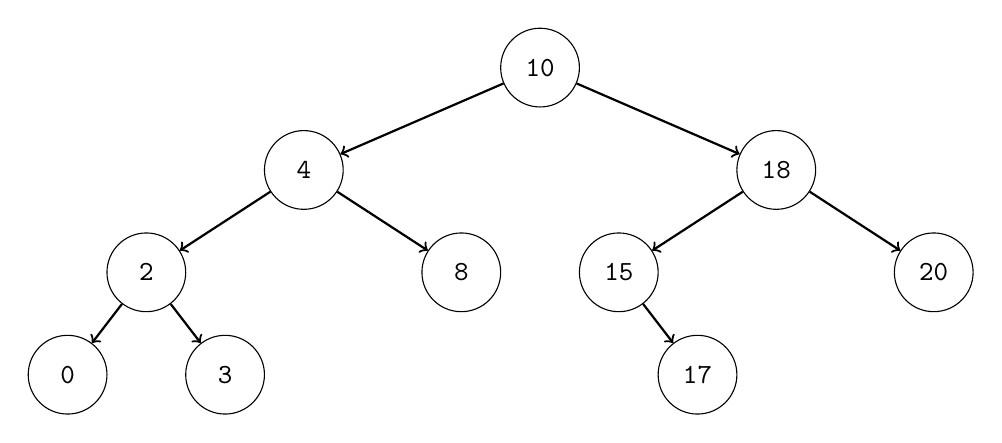
\begin{tikzpicture}
\node at (6,-1.3) [circle,draw,minimum size=10mm] (a) {\texttt{10}};
\node at (3,-2.6) [circle,draw,minimum size=10mm] (b) {\texttt{4}};
\node at (9,-2.6) [circle,draw,minimum size=10mm] (d) {\texttt{18}};
\node at (1,-3.9000000000000004) [circle,draw,minimum size=10mm] (e) {\texttt{2}};
\node at (5,-3.9000000000000004) [circle,draw,minimum size=10mm] (f) {\texttt{8}};
\node at (7,-3.9000000000000004) [circle,draw,minimum size=10mm] (h) {\texttt{15}};
\node at (11,-3.9000000000000004) [circle,draw,minimum size=10mm] (j) {\texttt{20}};
\node at (0,-5.2) [circle,draw,minimum size=10mm] (k) {\texttt{0}};
\node at (2,-5.2) [circle,draw,minimum size=10mm] (l) {\texttt{3}};
\node at (8,-5.2) [circle,draw,minimum size=10mm] (m) {\texttt{17}};
\draw [->,thick] (a) -- (b);
\draw [->,thick] (a) -- (d);
\draw [->,thick] (b) -- (e);
\draw [->,thick] (b) -- (f);
\draw [->,thick] (d) -- (h);
\draw [->,thick] (d) -- (j);
\draw [->,thick] (e) -- (k);
\draw [->,thick] (e) -- (l);
\draw [->,thick] (h) -- (m);

;
\end{tikzpicture}
    
\end{center}



Now this is not a maxheap. Do you see why?

I look at the children of \texttt{5}: \texttt{0} and \texttt{7}.
I swap \texttt{5} with the max of the children which is \texttt{7}


\begin{center}
\begin{tikzpicture}[>=triangle 60,shorten >=0.5pt,node distance=2cm,auto,initial text=, double distance=2pt]
\node[state] (A) at (  0,  0) {$0$};
\node[state] (B) at (  3,  0) {$1$};
\node[state] (F) at (  6,  0) {$2$};
\node[state] (C) at (  0, -2) {$3$};
\node[state] (D) at (  3, -2) {$4$};
\node[state] (E) at (  6, -2) {$5$};

\path[->]
(A) edge [loop above] node {} ()
(A) edge [bend left=0,pos=0.5,above] node {} (B)
(B) edge [bend left=0,pos=0.5] node {} (D)
(B) edge [bend left=0,pos=0.5,above] node {} (E)
(C) edge [bend left=0,pos=0.5,above] node {} (B)
(C) edge [bend left=0,pos=0.5,above] node {} (D)
(D) edge [bend left=0,pos=0.5,above] node {} (E)

;
\end{tikzpicture}
\end{center}
    


and get this:

\begin{center}
\begin{tikzpicture}

\fill[white] (18.0, -2.0) circle (0.3);
\node [line width=0.03cm,black,minimum size=0.57cm,draw,circle] at (18.0,-2.0)(A){};\draw (18.0, -2.0) node[color=black] {\texttt{20}};
\fill[white] (13.0, 0.0) circle (0.3);
\node [line width=0.03cm,black,minimum size=0.57cm,draw,circle] at (13.0,0.0)(a){};\draw (13.0, 0.0) node[color=black] {\texttt{10}};
\fill[white] (10.0, -1.0) circle (0.3);
\node [line width=0.03cm,black,minimum size=0.57cm,draw,circle] at (10.0,-1.0)(b){};\draw (10.0, -1.0) node[color=black] {\texttt{8}};
\fill[white] (16.0, -1.0) circle (0.3);
\node [line width=0.03cm,black,minimum size=0.57cm,draw,circle] at (16.0,-1.0)(p){};\draw (16.0, -1.0) node[color=black] {\texttt{18}};
\fill[white] (8.0, -2.0) circle (0.3);
\node [line width=0.03cm,black,minimum size=0.57cm,draw,circle] at (8.0,-2.0)(e){};\draw (8.0, -2.0) node[color=black] {\texttt{2}};
\fill[white] (7.0, -3.0) circle (0.3);
\node [line width=0.03cm,black,minimum size=0.57cm,draw,circle] at (7.0,-3.0)(k){};\draw (7.0, -3.0) node[color=black] {\texttt{0}};
\fill[white] (9.0, -3.0) circle (0.3);
\node [line width=0.03cm,black,minimum size=0.57cm,draw,circle] at (9.0,-3.0)(l){};\draw (9.0, -3.0) node[color=black] {\texttt{3}};
\fill[white] (14.0, -2.0) circle (0.3);
\node [line width=0.03cm,black,minimum size=0.57cm,draw,circle] at (14.0,-2.0)(h){};\draw (14.0, -2.0) node[color=black] {\texttt{15}};
\fill[white] (15.0, -3.0) circle (0.3);
\node [line width=0.03cm,black,minimum size=0.57cm,draw,circle] at (15.0,-3.0)(m){};\draw (15.0, -3.0) node[color=black] {\texttt{17}};\draw[line width=0.03cm,black,->,>=triangle 60] (a) to  (p);
\draw[line width=0.03cm,black,->,>=triangle 60] (h) to  (m);
\draw[line width=0.03cm,black,->,>=triangle 60] (a) to  (b);
\draw[line width=0.03cm,black,->,>=triangle 60] (p) to  (h);
\draw[line width=0.03cm,black,->,>=triangle 60] (p) to  (A);
\draw[line width=0.03cm,black,->,>=triangle 60] (b) to  (e);
\draw[line width=0.03cm,black,->,>=triangle 60] (e) to  (k);
\draw[line width=0.03cm,black,->,>=triangle 60] (e) to  (l);
\end{tikzpicture}

\end{center}



Clearly, we keep pushing \texttt{5} down as much as possible until
we get a maxheap again (i.e., heapify-down).
It might take more than one swap.

This above method works as long as \texttt{5} is a descendent of the
value to be removed.

Usually the value to be delete is in fact the root of the heap.
When the root is to be deleted, then the operation is called
\defone{extract-max} for the case of maxheap
and \defone{extract-min} for the case of
minheap.
I'm going to call both of them \defone{extract-root}.

Let's do another example.
Let's delete \texttt{20} (the root) from this maxheap:

\begin{center}
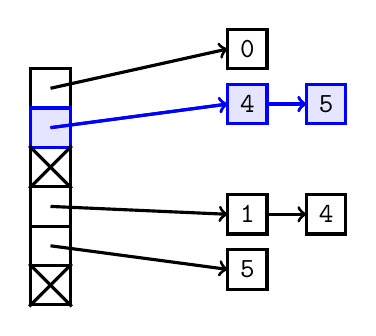
\begin{tikzpicture}

\draw (0.25, -0.25)
  node[draw, line width=0.04cm, , color=black,
       rounded corners=0cm, inner sep=0cm] {

\begin{minipage}[t][0.5cm]{0.5cm}
\mbox{}

\end{minipage}

};
\draw (0.25, -0.75)
  node[fill=blue!10,rounded corners=0cm,inner sep=0cm] {

\begin{minipage}[t][0.5cm]{0.5cm}
\mbox{}

\end{minipage}

};
\draw (0.25, -0.75)
  node[draw, line width=0.04cm, , color=blue,
       rounded corners=0cm, inner sep=0cm] {

\begin{minipage}[t][0.5cm]{0.5cm}
\mbox{}

\end{minipage}

};
\draw (0.25, -1.25)
  node[draw, line width=0.04cm, , color=black,
       rounded corners=0cm, inner sep=0cm] {

\begin{minipage}[t][0.5cm]{0.5cm}
\mbox{}

\end{minipage}

};
\draw (0.25, -1.75)
  node[draw, line width=0.04cm, , color=black,
       rounded corners=0cm, inner sep=0cm] {

\begin{minipage}[t][0.5cm]{0.5cm}
\mbox{}

\end{minipage}

};
\draw (0.25, -2.25)
  node[draw, line width=0.04cm, , color=black,
       rounded corners=0cm, inner sep=0cm] {

\begin{minipage}[t][0.5cm]{0.5cm}
\mbox{}

\end{minipage}

};
\draw (0.25, -2.75)
  node[draw, line width=0.04cm, , color=black,
       rounded corners=0cm, inner sep=0cm] {

\begin{minipage}[t][0.5cm]{0.5cm}
\mbox{}

\end{minipage}

};
\draw (0.25, -0.75)
  node[fill=blue!10,rounded corners=0cm,inner sep=0cm] {

\begin{minipage}[t][0.5cm]{0.5cm}
\mbox{}

\end{minipage}

};
\draw (0.25, -0.75)
  node[draw, line width=0.04cm, , color=blue,
       rounded corners=0cm, inner sep=0cm] {

\begin{minipage}[t][0.5cm]{0.5cm}
\mbox{}

\end{minipage}

};\draw[line width=0.04cm,black] (-0.02,-0.98) to  (0.52,-1.52);
\draw[line width=0.04cm,black] (0.52,-0.98) to  (-0.02,-1.52);
\draw[line width=0.04cm,black] (-0.02,-2.48) to  (0.52,-3.02);
\draw[line width=0.04cm,black] (0.52,-2.48) to  (-0.02,-3.02);

\draw (2.75, 0.24999999999999992)
  node[draw, line width=0.04cm, , color=black,
       rounded corners=0cm, inner sep=0cm] {

\begin{minipage}[t][0.5cm]{0.5cm}
\mbox{}

\end{minipage}

};\draw (2.75, 0.24999999999999992) node[color=black] {{\texttt{0}}};
\draw (2.75, -0.45000000000000007)
  node[fill=blue!10,rounded corners=0cm,inner sep=0cm] {

\begin{minipage}[t][0.5cm]{0.5cm}
\mbox{}

\end{minipage}

};
\draw (2.75, -0.45000000000000007)
  node[draw, line width=0.04cm, , color=blue,
       rounded corners=0cm, inner sep=0cm] {

\begin{minipage}[t][0.5cm]{0.5cm}
\mbox{}

\end{minipage}

};\draw (2.75, -0.45000000000000007) node[color=black] {{\texttt{4}}};
\draw (3.75, -0.45000000000000007)
  node[fill=blue!10,rounded corners=0cm,inner sep=0cm] {

\begin{minipage}[t][0.5cm]{0.5cm}
\mbox{}

\end{minipage}

};
\draw (3.75, -0.45000000000000007)
  node[draw, line width=0.04cm, , color=blue,
       rounded corners=0cm, inner sep=0cm] {

\begin{minipage}[t][0.5cm]{0.5cm}
\mbox{}

\end{minipage}

};\draw (3.75, -0.45000000000000007) node[color=black] {{\texttt{5}}};
\draw (2.75, -1.85)
  node[draw, line width=0.04cm, , color=black,
       rounded corners=0cm, inner sep=0cm] {

\begin{minipage}[t][0.5cm]{0.5cm}
\mbox{}

\end{minipage}

};\draw (2.75, -1.85) node[color=black] {{\texttt{1}}};
\draw (3.75, -1.85)
  node[draw, line width=0.04cm, , color=black,
       rounded corners=0cm, inner sep=0cm] {

\begin{minipage}[t][0.5cm]{0.5cm}
\mbox{}

\end{minipage}

};\draw (3.75, -1.85) node[color=black] {{\texttt{4}}};
\draw (2.75, -2.55)
  node[draw, line width=0.04cm, , color=black,
       rounded corners=0cm, inner sep=0cm] {

\begin{minipage}[t][0.5cm]{0.5cm}
\mbox{}

\end{minipage}

};\draw (2.75, -2.55) node[color=black] {{\texttt{5}}};
\draw (2.75, -0.45000000000000007)
  node[fill=blue!10,rounded corners=0cm,inner sep=0cm] {

\begin{minipage}[t][0.5cm]{0.5cm}
\mbox{}

\end{minipage}

};
\draw (2.75, -0.45000000000000007)
  node[draw, line width=0.04cm, , color=blue,
       rounded corners=0cm, inner sep=0cm] {

\begin{minipage}[t][0.5cm]{0.5cm}
\mbox{}

\end{minipage}

};\draw (2.75, -0.45000000000000007) node[color=black] {{\texttt{4}}};
\draw (3.75, -0.45000000000000007)
  node[fill=blue!10,rounded corners=0cm,inner sep=0cm] {

\begin{minipage}[t][0.5cm]{0.5cm}
\mbox{}

\end{minipage}

};
\draw (3.75, -0.45000000000000007)
  node[draw, line width=0.04cm, , color=blue,
       rounded corners=0cm, inner sep=0cm] {

\begin{minipage}[t][0.5cm]{0.5cm}
\mbox{}

\end{minipage}

};\draw (3.75, -0.45000000000000007) node[color=black] {{\texttt{5}}};\draw[line width=0.04cm,black,->] (0.25,-0.25) to  (2.5,0.25);
\draw[line width=0.04cm,blue,->] (0.25,-0.75) to  (2.5,-0.45);
\draw[line width=0.04cm,blue,->] (3.0,-0.45) to  (3.5,-0.45);
\draw[line width=0.04cm,black,->] (0.25,-1.75) to  (2.5,-1.85);
\draw[line width=0.04cm,black,->] (3.0,-1.85) to  (3.5,-1.85);
\draw[line width=0.04cm,black,->] (0.25,-2.25) to  (2.5,-2.55);
\draw[line width=0.04cm,blue,->] (0.25,-0.75) to  (2.5,-0.45);
\draw[line width=0.04cm,blue,->] (3.0,-0.45) to  (3.5,-0.45);
\end{tikzpicture}

\end{center}




Again, I overwrite \texttt{20} with \texttt{5}

\input{stdout41.tex}

(\texttt{5} is chosen, again because it's the rightmost
in the last level, or equivalently, it's the last in the
corresponding array implementation.)
I get this:

\begin{center}
\begin{tikzpicture}

\fill[white] (19.0, -0.6) circle (0.3);
\node [line width=0.03cm,black,minimum size=0.57cm,draw,circle] at (19.0,-0.6)(A){};\draw (19.0, -0.6) node[color=black] {\texttt{20}};
\fill[white] (16.0, -1.0) circle (0.3);
\node [line width=0.03cm,black,minimum size=0.57cm,draw,circle] at (16.0,-1.0)(a){};\draw (16.0, -1.0) node[color=black] {\texttt{10}};
\fill[white] (10.0, -2.0) circle (0.3);
\node [line width=0.03cm,black,minimum size=0.57cm,draw,circle] at (10.0,-2.0)(b){};\draw (10.0, -2.0) node[color=black] {\texttt{0}};
\fill[white] (11.0, -4.0) circle (0.3);
\node [line width=0.03cm,black,minimum size=0.57cm,draw,circle] at (11.0,-4.0)(d){};\draw (11.0, -4.0) node[color=black] {\texttt{18}};
\fill[white] (8.0, -3.0) circle (0.3);
\node [line width=0.03cm,black,minimum size=0.57cm,draw,circle] at (8.0,-3.0)(e){};\draw (8.0, -3.0) node[color=black] {\texttt{-2}};
\fill[white] (7.0, -4.0) circle (0.3);
\node [line width=0.03cm,black,minimum size=0.57cm,draw,circle] at (7.0,-4.0)(k){};\draw (7.0, -4.0) node[color=black] {\texttt{-3}};
\fill[white] (9.0, -4.0) circle (0.3);
\node [line width=0.03cm,black,minimum size=0.57cm,draw,circle] at (9.0,-4.0)(l){};\draw (9.0, -4.0) node[color=black] {\texttt{-1}};
\fill[white] (15.0, -4.0) circle (0.3);
\node [line width=0.03cm,black,minimum size=0.57cm,draw,circle] at (15.0,-4.0)(h){};\draw (15.0, -4.0) node[color=black] {\texttt{8}};
\fill[white] (14.0, -5.0) circle (0.3);
\node [line width=0.03cm,black,minimum size=0.57cm,draw,circle] at (14.0,-5.0)(m){};\draw (14.0, -5.0) node[color=black] {\texttt{6}};
\fill[white] (13.0, -3.0) circle (0.3);
\node [line width=0.03cm,black,minimum size=0.57cm,draw,circle] at (13.0,-3.0)(f){};\draw (13.0, -3.0) node[color=black] {\texttt{5}};
\fill[white] (13.0, -6.0) circle (0.3);
\node [line width=0.03cm,black,minimum size=0.57cm,draw,circle] at (13.0,-6.0)(n){};\draw (13.0, -6.0) node[color=black] {\texttt{4}};
\fill[white] (15.0, -6.0) circle (0.3);
\node [line width=0.03cm,black,minimum size=0.57cm,draw,circle] at (15.0,-6.0)(o){};\draw (15.0, -6.0) node[color=black] {\texttt{7}};
\fill[white] (18.0, -2.0) circle (0.3);
\node [line width=0.03cm,black,minimum size=0.57cm,draw,circle] at (18.0,-2.0)(p){};\draw (18.0, -2.0) node[color=black] {\texttt{15}};\draw[line width=0.03cm,black,->,>=triangle 60] (A) to  (a);
\draw[line width=0.03cm,black,->,>=triangle 60] (a) to  (p);
\draw[line width=0.03cm,black,->,>=triangle 60] (a) to  (b);
\draw[line width=0.03cm,black,->,>=triangle 60] (b) to  (e);
\draw[line width=0.03cm,black,->,>=triangle 60] (b) to  (f);
\draw[line width=0.03cm,black,->,>=triangle 60] (f) to  (d);
\draw[line width=0.03cm,black,->,>=triangle 60] (f) to  (h);
\draw[line width=0.03cm,black,->,>=triangle 60] (e) to  (k);
\draw[line width=0.03cm,black,->,>=triangle 60] (e) to  (l);
\draw[line width=0.03cm,black,->,>=triangle 60] (h) to  (m);
\draw[line width=0.03cm,black,->,>=triangle 60] (m) to  (n);
\draw[line width=0.03cm,black,->,>=triangle 60] (m) to  (o);
\end{tikzpicture}

\end{center}



I do the same again as above: I pick the larger of the children
of \texttt{5}, which in this case is \texttt{10} and swap with \texttt{5}.
I get this:

from latextool_basic import *
print(automata(layout="""
A  B

C  D
""",
edges="A,$a$,B|A,$b$,C|B,$a$,D|B,$b$,C|C,$b$,A|C,$a$,D|D,$a$,B|D,$b$,A",
A='initial|label=$q_0$',
B='accept|label=$q_1$',
C='label=$q_2$',
D='accept|label=$q_3$', xscale=1.3,
))


It's not a maxheap yet.
I look at the children of \texttt{5} and choose the largest,
which would be \texttt{9}, and swap it with \texttt{5}.
Here's what I get:

\begin{center}
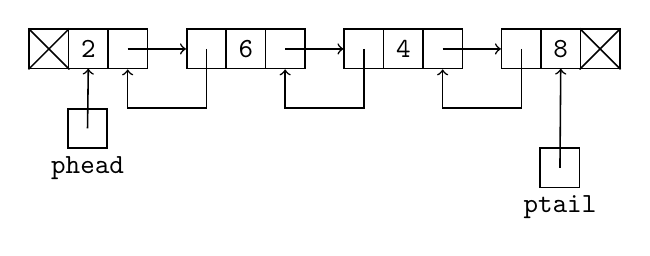
\begin{tikzpicture}

\draw (0.25, 0.25)
  node[draw, line width=0.02cm, , color=black,
       rounded corners=0cm, inner sep=0cm] {

\begin{minipage}[t][0.5cm]{0.5cm}
\mbox{}

\end{minipage}

};\draw (0.25, 0.25) node[color=black] {{\texttt{}}};
\draw (0.75, 0.25)
  node[draw, line width=0.02cm, , color=black,
       rounded corners=0cm, inner sep=0cm] {

\begin{minipage}[t][0.5cm]{0.5cm}
\mbox{}

\end{minipage}

};\draw (0.75, 0.25) node[color=black] {{\texttt{2}}};
\draw (1.25, 0.25)
  node[draw, line width=0.02cm, , color=black,
       rounded corners=0cm, inner sep=0cm] {

\begin{minipage}[t][0.5cm]{0.5cm}
\mbox{}

\end{minipage}

};\draw (1.25, 0.25) node[color=black] {{\texttt{}}};
\draw (2.25, 0.25)
  node[draw, line width=0.02cm, , color=black,
       rounded corners=0cm, inner sep=0cm] {

\begin{minipage}[t][0.5cm]{0.5cm}
\mbox{}

\end{minipage}

};\draw (2.25, 0.25) node[color=black] {{\texttt{}}};
\draw (2.75, 0.25)
  node[draw, line width=0.02cm, , color=black,
       rounded corners=0cm, inner sep=0cm] {

\begin{minipage}[t][0.5cm]{0.5cm}
\mbox{}

\end{minipage}

};\draw (2.75, 0.25) node[color=black] {{\texttt{6}}};
\draw (3.25, 0.25)
  node[draw, line width=0.02cm, , color=black,
       rounded corners=0cm, inner sep=0cm] {

\begin{minipage}[t][0.5cm]{0.5cm}
\mbox{}

\end{minipage}

};\draw (3.25, 0.25) node[color=black] {{\texttt{}}};
\draw (4.25, 0.25)
  node[draw, line width=0.02cm, , color=black,
       rounded corners=0cm, inner sep=0cm] {

\begin{minipage}[t][0.5cm]{0.5cm}
\mbox{}

\end{minipage}

};\draw (4.25, 0.25) node[color=black] {{\texttt{}}};
\draw (4.75, 0.25)
  node[draw, line width=0.02cm, , color=black,
       rounded corners=0cm, inner sep=0cm] {

\begin{minipage}[t][0.5cm]{0.5cm}
\mbox{}

\end{minipage}

};\draw (4.75, 0.25) node[color=black] {{\texttt{4}}};
\draw (5.25, 0.25)
  node[draw, line width=0.02cm, , color=black,
       rounded corners=0cm, inner sep=0cm] {

\begin{minipage}[t][0.5cm]{0.5cm}
\mbox{}

\end{minipage}

};\draw (5.25, 0.25) node[color=black] {{\texttt{}}};
\draw (6.25, 0.25)
  node[draw, line width=0.02cm, , color=black,
       rounded corners=0cm, inner sep=0cm] {

\begin{minipage}[t][0.5cm]{0.5cm}
\mbox{}

\end{minipage}

};\draw (6.25, 0.25) node[color=black] {{\texttt{}}};
\draw (6.75, 0.25)
  node[draw, line width=0.02cm, , color=black,
       rounded corners=0cm, inner sep=0cm] {

\begin{minipage}[t][0.5cm]{0.5cm}
\mbox{}

\end{minipage}

};\draw (6.75, 0.25) node[color=black] {{\texttt{8}}};
\draw (7.25, 0.25)
  node[draw, line width=0.02cm, , color=black,
       rounded corners=0cm, inner sep=0cm] {

\begin{minipage}[t][0.5cm]{0.5cm}
\mbox{}

\end{minipage}

};\draw (7.25, 0.25) node[color=black] {{\texttt{}}};\draw[line width=0.02cm,black,->] (1.25,0.25) to  (1.99,0.25);
\draw[line width=0.02cm,black,->] (3.25,0.25) to  (3.99,0.25);
\draw[line width=0.02cm,black,->] (2.25,0.25) to  (2.25,-0.5) to  (1.25,-0.5) to  (1.25,-0.01);
\draw[line width=0.02cm,black,->] (5.25,0.25) to  (5.99,0.25);
\draw[line width=0.02cm,black,->] (4.25,0.25) to  (4.25,-0.5) to  (3.25,-0.5) to  (3.25,-0.01);
\draw[line width=0.02cm,black,->] (6.25,0.25) to  (6.25,-0.5) to  (5.25,-0.5) to  (5.25,-0.01);
\draw[line width=0.02cm,black] (-0.01,0.51) to  (0.51,-0.01);
\draw[line width=0.02cm,black] (0.51,0.51) to  (-0.01,-0.01);
\draw[line width=0.02cm,black] (6.99,0.51) to  (7.51,-0.01);
\draw[line width=0.02cm,black] (7.51,0.51) to  (6.99,-0.01);

\draw (0.74, -0.76)
  node[draw, line width=0.02cm, , color=black,
       rounded corners=0cm, inner sep=0cm] {

\begin{minipage}[t][0.5cm]{0.5cm}
\mbox{}

\end{minipage}

};\draw (0.74, -0.76) node[color=black] {{\texttt{}}};
\draw (0.74, -1.26)
  node[draw, line width=0.02cm, , color=white,
       rounded corners=0cm, inner sep=0cm] {

\begin{minipage}[t][0.1cm]{0.1cm}
\mbox{}

\end{minipage}

};\draw (0.74, -1.26) node[color=black] {{\texttt{phead}}};\draw[line width=0.02cm,black,->] (0.74,-0.76) to  (0.75,0);

\draw (6.74, -1.26)
  node[draw, line width=0.02cm, , color=black,
       rounded corners=0cm, inner sep=0cm] {

\begin{minipage}[t][0.5cm]{0.5cm}
\mbox{}

\end{minipage}

};\draw (6.74, -1.26) node[color=black] {{\texttt{}}};
\draw (6.74, -1.76)
  node[draw, line width=0.02cm, , color=white,
       rounded corners=0cm, inner sep=0cm] {

\begin{minipage}[t][0.1cm]{0.1cm}
\mbox{}

\end{minipage}

};\draw (6.74, -1.76) node[color=black] {{\texttt{ptail}}};\draw[line width=0.02cm,black,->] (6.74,-1.26) to  (6.75,0);
\end{tikzpicture}

\end{center}



Ahhh ... at this point I have a maxheap.
I'm done!

\begin{console}[commandchars=\\\{\}]
  ALGORITHM: heap_delete (for maxheap)
  INPUT: x - an array representing a maxheap
  n - the length of the heap in x (pass by reference)
  i - index of value to be removed (note usually
  this is 0)

  x[i] = x[n - 1]
  n = n - 1
  heapify_down(x, i)
\end{console}

(Note that because of the shape of the tree -- a complete tree --
a node cannot have a right child but no left child.)

Recall what I just said: usually the delete operation for maxheap
occurs at index 0, i.e., you're removing the maximum value in the maxheap.
In that case the operation is also called extract-max or delete-max.
You'll see why when we use this delete operation to perform heapsort
and when we use this for priority queues.

Note that the runtime is
\[
  O(\log n)
\]
since the heapify-down operation basically moves
a value in the tree down to the leaf level, possibly stopping
early.
This means that the worse runtime must be
the height of the tree which is $O(\log n)$.

\newpage
\begin{ex}
  You are given this maxheap:

  \begin{center}
\begin{tikzpicture}

\fill[white] (19.0, -0.6) circle (0.3);
\node [line width=0.03cm,black,minimum size=0.57cm,draw,circle] at (19.0,-0.6)(A){};\draw (19.0, -0.6) node[color=black] {\texttt{20}};
\fill[white] (16.0, -1.0) circle (0.3);
\node [line width=0.03cm,black,minimum size=0.57cm,draw,circle] at (16.0,-1.0)(a){};\draw (16.0, -1.0) node[color=black] {\texttt{10}};\draw[line width=0.1cm,black] (15.8,-1.2) to  (16.2,-0.8);

\fill[white] (16.0, -2.0) circle (0.3);
\node [line width=0.03cm,white,minimum size=0.57cm,draw,circle] at (16.0,-2.0)(aa){};\draw (16.0, -2.0) node[color=black] {\texttt{0}};\draw[line width=0.05cm,black,->,>=triangle 60] (aa) to  (a);

\fill[white] (10.0, -2.0) circle (0.3);
\node [line width=0.03cm,black,,dashed,minimum size=0.57cm,draw,circle] at (10.0,-2.0)(b){};\draw (10.0, -2.0) node[color=black] {\texttt{0}};
\fill[white] (8.0, -3.0) circle (0.3);
\node [line width=0.03cm,black,minimum size=0.57cm,draw,circle] at (8.0,-3.0)(e){};\draw (8.0, -3.0) node[color=black] {\texttt{-2}};
\fill[white] (7.0, -4.0) circle (0.3);
\node [line width=0.03cm,black,minimum size=0.57cm,draw,circle] at (7.0,-4.0)(k){};\draw (7.0, -4.0) node[color=black] {\texttt{-3}};
\fill[white] (9.0, -4.0) circle (0.3);
\node [line width=0.03cm,black,minimum size=0.57cm,draw,circle] at (9.0,-4.0)(l){};\draw (9.0, -4.0) node[color=black] {\texttt{-1}};
\fill[white] (18.0, -2.0) circle (0.3);
\node [line width=0.03cm,black,minimum size=0.57cm,draw,circle] at (18.0,-2.0)(p){};\draw (18.0, -2.0) node[color=black] {\texttt{15}};\draw[line width=0.03cm,black,->,>=triangle 60] (a) to  (e);
\draw[line width=0.03cm,black,->,>=triangle 60] (A) to  (a);
\draw[line width=0.03cm,black,->,>=triangle 60] (a) to  (p);
\draw[line width=0.03cm,black,->,>=triangle 60] (e) to  (k);
\draw[line width=0.03cm,black,->,>=triangle 60] (e) to  (l);
\draw[line width=0.03cm,black,->,>=triangle 60,dashed] (a) to  (b);
\draw[line width=0.03cm,black,->,>=triangle 60,dashed] (b) to  (e);
\end{tikzpicture}

\end{center}



  Do the following operations one after another,
  drawing the tree including the swaps
  and the final
  maxheap.
  Also, draw the corresponding array.
  \begin{tightlist}
  \item Delete \texttt{28}.
  \item Delete \texttt{34}
  \item Delete \texttt{16}
  \item Delete the maximum value in the maxheap, i.e., perform extract max.
  \item Delete the maximum value in the maxheap, i.e., perform extract max.
  \end{tightlist}
\end{ex}

\newpage
\begin{ex}
  Draw a minheap with 15 distinct values.
  Extract the minimum and draw the minheap.
  Do it again.
  \qed
\end{ex}





\begin{ex}
  Using an array, 
  build a maxheap by inserting the following into an empty tree:
  1, 3, 5, 7, 6, 4, 2, 0, 8, 9.
  Make sure the tree is complete after each insert and the leaves
  at the lowest level are all on the left.
  Call the array \texttt{x}
  (assume it has size at least 10)
  and use integer variable \texttt{len}
  for the length of \texttt{x}.
  Of course initially \texttt{len} is 0.
  \qed
\end{ex}

\begin{ex}
  Using the maxheap (using an array) from the previous question,
  remove the following values one after another left to right:
  \[
    1, 3, 5, 7, 6, 4, 2, 0, 8, 9
  \]
  Call the array \texttt{x} and use integer variable \texttt{len}
  for the length of \texttt{x}.
  Of course initially \texttt{len} is 10.
  Make sure that after each delete, the tree is complete after each delete and 
  the leaves
  at the lowest level are all on the left.
  \qed
\end{ex}

\begin{ex}
  Suppose during an extract-root for minheap,
  you need to heapify-down at an index \verb!i!.
  Suppose the left and right child value of \verb!x[i]! are the same and
  larger than \verb!x[i]!.
  Which do you prefer to swap with \verb!x[i]!, the left or the right
  child?
\end{ex}
% choose the right because the tree might be one step shorter on the right
% and therefore the heapify down might terminate earlier by 1 step
%
% Example:
%     5
%    1 1
%   3

\begin{ex}
  Suppose you have a heap whose array is \verb!x!.
  In this heap, if you extract the root and you insert the same value back
  into the heap, will the heap be the same as the original \verb!x!?
  \qed
\end{ex}
%NO
%    1
%  2   3
%
%    2
%  3
%
%    2      --->      1
%  3   1            3   2
%

\newpage%-*-latex-*-
\section{Heap and complete trees}

Recall that we have complete freedom in choosing where to insert a new node.
We also have complete freedom in choosing any leaf to use to overwrite
a node to be deleted as long as the leaf is a descendent of the node whose
value is to delete.
In particular, if we are remove the value of the root of the heap,
we can choose any leaf.

It's because of the above,
after every insert and root value removal,
we can alway ensure that the heap is complete.
Recall that a complete binary tree that is almost full except that the
last level might not have all the leaves.
are at the same level.
Furthermore, we can force to have
all the leaves to be all on the left side of the whole
tree.
This is what I mean by \lq\lq left side'' of the tree:

\begin{python}
from latextool_basic import *
print(r"""
\begin{center}
%s
\end{center}
""" % graph(yscale=1, xscale=1,
layout="""
      A 
   B     C
 D   E F   G
H I J
""",
minimum_size='8mm',
edges='A-B,A-C,B-D,B-E,C-G,C-F,D-H,D-I,E-J',
A=r'label=',
B=r'label=',
C=r'label=',
D=r'label=',
E=r'label=',
F=r'label=',
G=r'label=',
H=r'label=',
I=r'label=',
J=r'label=',
))
\end{python}

This can be achieved by
\begin{tightlist}
\li During insert, always insert a leaf just to the right of the
rightmost leaf at the last level.
\li During delete, always using the right most leaf of the 
last level whenever we remove the root.
\end{tightlist}




\newpage
\begin{ex}
Build a maxheap by inserting the following into an empty tree:
1, 3, 5, 7, 6, 4, 2, 8, 9, 0.
Make sure the tree is complete after each insert and the leaves
at the lowest level are all on the left.
\qed
\end{ex}

\newpage
\begin{ex}
Using the maxheap from the previous question,
remove the following values one after another:
1, 3, 5, 7, 6, 4, 2, 8, 9, 0.
Make sure that after each delete, the tree is complete after each insert and the leaves
at the lowest level are all on the left.
\qed
\end{ex}

\newpage
\begin{ex}
  Suppose that in maxheap, there are two 5's.
  One 5 was inserted at 9AM and the second 5 was inserted
  at 10AM.
  If I delete the maximum value of the heap
  until the heap is empty,
  will the 5 inserted at 9AM be deleted
  from the heap
  before or after the 5 inserted at 10AM?
  Or are both scenarios possible?
\end{ex}

\newpage
Being complete means that the heaps can have the minimal possible height.
At this point, you ought to know that this is a good thing.

This also implies right away that the worse runtimes for 
insert and delete is $O(\log n)$ for both insert and delete
as long as we keep the heap complete.


\newpage%-*-latex-*-
\sectionthree{Increase-key and decrease-key}
\begin{python0}
from solutions import *; clear()
\end{python0}

So suppose I already have a priority queue (as a heap):

\begin{center}
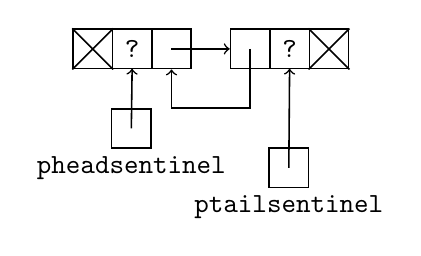
\begin{tikzpicture}

\draw (0.25, 0.25)
  node[draw, line width=0.02cm, , color=black,
       rounded corners=0cm, inner sep=0cm] {

\begin{minipage}[t][0.5cm]{0.5cm}
\mbox{}

\end{minipage}

};\draw (0.25, 0.25) node[color=black] {{\texttt{}}};
\draw (0.75, 0.25)
  node[draw, line width=0.02cm, , color=black,
       rounded corners=0cm, inner sep=0cm] {

\begin{minipage}[t][0.5cm]{0.5cm}
\mbox{}

\end{minipage}

};\draw (0.75, 0.25) node[color=black] {{\texttt{?}}};
\draw (1.25, 0.25)
  node[draw, line width=0.02cm, , color=black,
       rounded corners=0cm, inner sep=0cm] {

\begin{minipage}[t][0.5cm]{0.5cm}
\mbox{}

\end{minipage}

};\draw (1.25, 0.25) node[color=black] {{\texttt{}}};
\draw (2.25, 0.25)
  node[draw, line width=0.02cm, , color=black,
       rounded corners=0cm, inner sep=0cm] {

\begin{minipage}[t][0.5cm]{0.5cm}
\mbox{}

\end{minipage}

};\draw (2.25, 0.25) node[color=black] {{\texttt{}}};
\draw (2.75, 0.25)
  node[draw, line width=0.02cm, , color=black,
       rounded corners=0cm, inner sep=0cm] {

\begin{minipage}[t][0.5cm]{0.5cm}
\mbox{}

\end{minipage}

};\draw (2.75, 0.25) node[color=black] {{\texttt{?}}};
\draw (3.25, 0.25)
  node[draw, line width=0.02cm, , color=black,
       rounded corners=0cm, inner sep=0cm] {

\begin{minipage}[t][0.5cm]{0.5cm}
\mbox{}

\end{minipage}

};\draw (3.25, 0.25) node[color=black] {{\texttt{}}};\draw[line width=0.02cm,black,->] (1.25,0.25) to  (1.99,0.25);
\draw[line width=0.02cm,black,->] (2.25,0.25) to  (2.25,-0.5) to  (1.25,-0.5) to  (1.25,-0.01);
\draw[line width=0.02cm,black] (-0.01,0.51) to  (0.51,-0.01);
\draw[line width=0.02cm,black] (0.51,0.51) to  (-0.01,-0.01);
\draw[line width=0.02cm,black] (2.99,0.51) to  (3.51,-0.01);
\draw[line width=0.02cm,black] (3.51,0.51) to  (2.99,-0.01);

\draw (0.74, -0.76)
  node[draw, line width=0.02cm, , color=black,
       rounded corners=0cm, inner sep=0cm] {

\begin{minipage}[t][0.5cm]{0.5cm}
\mbox{}

\end{minipage}

};\draw (0.74, -0.76) node[color=black] {{\texttt{}}};
\draw (0.74, -1.26)
  node[draw, line width=0.02cm, , color=white,
       rounded corners=0cm, inner sep=0cm] {

\begin{minipage}[t][0.1cm]{0.1cm}
\mbox{}

\end{minipage}

};\draw (0.74, -1.26) node[color=black] {{\texttt{pheadsentinel}}};\draw[line width=0.02cm,black,->] (0.74,-0.76) to  (0.75,0);

\draw (2.74, -1.26)
  node[draw, line width=0.02cm, , color=black,
       rounded corners=0cm, inner sep=0cm] {

\begin{minipage}[t][0.5cm]{0.5cm}
\mbox{}

\end{minipage}

};\draw (2.74, -1.26) node[color=black] {{\texttt{}}};
\draw (2.74, -1.76)
  node[draw, line width=0.02cm, , color=white,
       rounded corners=0cm, inner sep=0cm] {

\begin{minipage}[t][0.1cm]{0.1cm}
\mbox{}

\end{minipage}

};\draw (2.74, -1.76) node[color=black] {{\texttt{ptailsentinel}}};\draw[line width=0.02cm,black,->] (2.74,-1.26) to  (2.75,0);
\end{tikzpicture}

\end{center}




Suppose \texttt{1} is increased to \texttt{12}:

\begin{center}
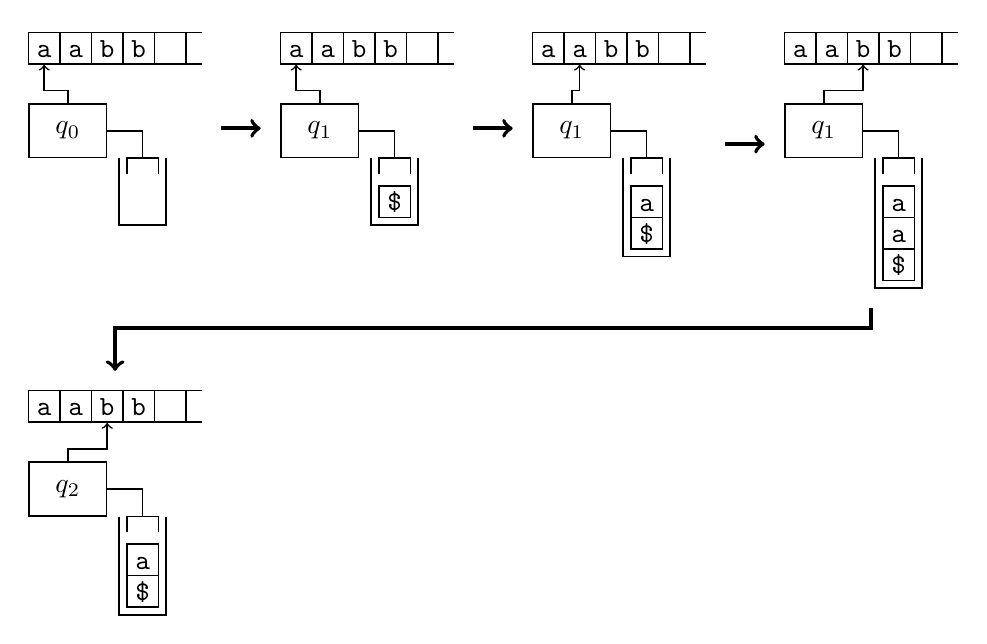
\begin{tikzpicture}

\draw (0.2, 0.2)
  node[draw, line width=0.02cm, , color=black,
       rounded corners=0cm, inner sep=0cm] {

\begin{minipage}[t][0.4cm]{0.4cm}
\mbox{}

\end{minipage}

};\draw (0.2, 0.2) node[color=black] {{\vphantom{aabb\SPACE}\texttt{a}}};
\draw (0.6000000000000001, 0.2)
  node[draw, line width=0.02cm, , color=black,
       rounded corners=0cm, inner sep=0cm] {

\begin{minipage}[t][0.4cm]{0.4cm}
\mbox{}

\end{minipage}

};\draw (0.6000000000000001, 0.2) node[color=black] {{\vphantom{aabb\SPACE}\texttt{a}}};
\draw (1.0, 0.2)
  node[draw, line width=0.02cm, , color=black,
       rounded corners=0cm, inner sep=0cm] {

\begin{minipage}[t][0.4cm]{0.4cm}
\mbox{}

\end{minipage}

};\draw (1.0, 0.2) node[color=black] {{\vphantom{aabb\SPACE}\texttt{b}}};
\draw (1.4000000000000001, 0.2)
  node[draw, line width=0.02cm, , color=black,
       rounded corners=0cm, inner sep=0cm] {

\begin{minipage}[t][0.4cm]{0.4cm}
\mbox{}

\end{minipage}

};\draw (1.4000000000000001, 0.2) node[color=black] {{\vphantom{aabb\SPACE}\texttt{b}}};
\draw (1.7999999999999998, 0.2)
  node[draw, line width=0.02cm, , color=black,
       rounded corners=0cm, inner sep=0cm] {

\begin{minipage}[t][0.4cm]{0.4cm}
\mbox{}

\end{minipage}

};\draw (1.7999999999999998, 0.2) node[color=black] {{\vphantom{aabb\SPACE}\texttt{\SPACE}}};\draw[line width=0.02cm,black] (2.0,0.4) to  (2.2,0.4);
\draw[line width=0.02cm,black] (2.0,0.0) to  (2.2,0.0);

\draw (0.5, -0.85)
  node[draw, line width=0.02cm, , color=black,
       rounded corners=0cm, inner sep=0cm] {

\begin{minipage}[t][0.68cm]{0.98cm}
\mbox{}

\end{minipage}

};\draw (0.5, -0.85) node[color=black] {$q_0$};\draw[line width=0.02cm,black,->] (0.5,-0.5) to  (0.5,-0.34) to  (0.2,-0.34) to  (0.2,-0.01);

\draw (1.45, -1.7499999999999998)
  node[draw=none, line width=0cm, , color=black,
       rounded corners=0cm, inner sep=0cm] {

\begin{minipage}[t][0.4cm]{0.4cm}
\mbox{}

\end{minipage}

};\draw[line width=0.02cm,black] (1.15,-1.2) to  (1.15,-2.05) to  (1.75,-2.05) to  (1.75,-1.2);
\draw[line width=0.02cm,black] (1,-0.85) to  (1.45,-0.85) to  (1.45,-1.2);
\draw[line width=0.02cm,black] (1.25,-1.4) to  (1.25,-1.2) to  (1.65,-1.2) to  (1.65,-1.4);
\draw[line width=0.05cm,black,->] (2.45,-0.82) to  (2.95,-0.82);

\draw (3.4000000000000004, 0.2)
  node[draw, line width=0.02cm, , color=black,
       rounded corners=0cm, inner sep=0cm] {

\begin{minipage}[t][0.4cm]{0.4cm}
\mbox{}

\end{minipage}

};\draw (3.4000000000000004, 0.2) node[color=black] {{\vphantom{\$aabb\SPACE}\texttt{a}}};
\draw (3.8, 0.2)
  node[draw, line width=0.02cm, , color=black,
       rounded corners=0cm, inner sep=0cm] {

\begin{minipage}[t][0.4cm]{0.4cm}
\mbox{}

\end{minipage}

};\draw (3.8, 0.2) node[color=black] {{\vphantom{\$aabb\SPACE}\texttt{a}}};
\draw (4.2, 0.2)
  node[draw, line width=0.02cm, , color=black,
       rounded corners=0cm, inner sep=0cm] {

\begin{minipage}[t][0.4cm]{0.4cm}
\mbox{}

\end{minipage}

};\draw (4.2, 0.2) node[color=black] {{\vphantom{\$aabb\SPACE}\texttt{b}}};
\draw (4.6000000000000005, 0.2)
  node[draw, line width=0.02cm, , color=black,
       rounded corners=0cm, inner sep=0cm] {

\begin{minipage}[t][0.4cm]{0.4cm}
\mbox{}

\end{minipage}

};\draw (4.6000000000000005, 0.2) node[color=black] {{\vphantom{\$aabb\SPACE}\texttt{b}}};
\draw (5.000000000000001, 0.2)
  node[draw, line width=0.02cm, , color=black,
       rounded corners=0cm, inner sep=0cm] {

\begin{minipage}[t][0.4cm]{0.4cm}
\mbox{}

\end{minipage}

};\draw (5.000000000000001, 0.2) node[color=black] {{\vphantom{\$aabb\SPACE}\texttt{\SPACE}}};\draw[line width=0.02cm,black] (5.200000000000001,0.4) to  (5.4,0.4);
\draw[line width=0.02cm,black] (5.200000000000001,0.0) to  (5.4,0.0);

\draw (3.7, -0.85)
  node[draw, line width=0.02cm, , color=black,
       rounded corners=0cm, inner sep=0cm] {

\begin{minipage}[t][0.68cm]{0.98cm}
\mbox{}

\end{minipage}

};\draw (3.7, -0.85) node[color=black] {$q_1$};\draw[line width=0.02cm,black,->] (3.7,-0.5) to  (3.7,-0.34) to  (3.4,-0.34) to  (3.4,-0.01);

\draw (4.65, -1.7499999999999998)
  node[draw, line width=0.02cm, , color=black,
       rounded corners=0cm, inner sep=0cm] {

\begin{minipage}[t][0.4cm]{0.4cm}
\mbox{}

\end{minipage}

};\draw (4.65, -1.7499999999999998) node[color=black] {{\vphantom{\$aabb\SPACE}\texttt{\$}}};\draw[line width=0.02cm,black] (4.35,-1.2) to  (4.35,-2.05) to  (4.95,-2.05) to  (4.95,-1.2);
\draw[line width=0.02cm,black] (4.2,-0.85) to  (4.65,-0.85) to  (4.65,-1.2);
\draw[line width=0.02cm,black] (4.45,-1.4) to  (4.45,-1.2) to  (4.85,-1.2) to  (4.85,-1.4);
\draw[line width=0.05cm,black,->] (5.65,-0.82) to  (6.15,-0.82);

\draw (6.600000000000001, 0.2)
  node[draw, line width=0.02cm, , color=black,
       rounded corners=0cm, inner sep=0cm] {

\begin{minipage}[t][0.4cm]{0.4cm}
\mbox{}

\end{minipage}

};\draw (6.600000000000001, 0.2) node[color=black] {{\vphantom{a\$aabb\SPACE}\texttt{a}}};
\draw (7.000000000000002, 0.2)
  node[draw, line width=0.02cm, , color=black,
       rounded corners=0cm, inner sep=0cm] {

\begin{minipage}[t][0.4cm]{0.4cm}
\mbox{}

\end{minipage}

};\draw (7.000000000000002, 0.2) node[color=black] {{\vphantom{a\$aabb\SPACE}\texttt{a}}};
\draw (7.400000000000002, 0.2)
  node[draw, line width=0.02cm, , color=black,
       rounded corners=0cm, inner sep=0cm] {

\begin{minipage}[t][0.4cm]{0.4cm}
\mbox{}

\end{minipage}

};\draw (7.400000000000002, 0.2) node[color=black] {{\vphantom{a\$aabb\SPACE}\texttt{b}}};
\draw (7.8000000000000025, 0.2)
  node[draw, line width=0.02cm, , color=black,
       rounded corners=0cm, inner sep=0cm] {

\begin{minipage}[t][0.4cm]{0.4cm}
\mbox{}

\end{minipage}

};\draw (7.8000000000000025, 0.2) node[color=black] {{\vphantom{a\$aabb\SPACE}\texttt{b}}};
\draw (8.200000000000003, 0.2)
  node[draw, line width=0.02cm, , color=black,
       rounded corners=0cm, inner sep=0cm] {

\begin{minipage}[t][0.4cm]{0.4cm}
\mbox{}

\end{minipage}

};\draw (8.200000000000003, 0.2) node[color=black] {{\vphantom{a\$aabb\SPACE}\texttt{\SPACE}}};\draw[line width=0.02cm,black] (8.400000000000002,0.4) to  (8.600000000000001,0.4);
\draw[line width=0.02cm,black] (8.400000000000002,0.0) to  (8.600000000000001,0.0);

\draw (6.900000000000001, -0.85)
  node[draw, line width=0.02cm, , color=black,
       rounded corners=0cm, inner sep=0cm] {

\begin{minipage}[t][0.68cm]{0.98cm}
\mbox{}

\end{minipage}

};\draw (6.900000000000001, -0.85) node[color=black] {$q_1$};\draw[line width=0.02cm,black,->] (6.9,-0.5) to  (6.9,-0.34) to  (7.0,-0.34) to  (7.0,-0.01);

\draw (7.850000000000001, -1.7499999999999998)
  node[draw, line width=0.02cm, , color=black,
       rounded corners=0cm, inner sep=0cm] {

\begin{minipage}[t][0.4cm]{0.4cm}
\mbox{}

\end{minipage}

};\draw (7.850000000000001, -1.7499999999999998) node[color=black] {{\vphantom{a\$aabb\SPACE}\texttt{a}}};
\draw (7.850000000000001, -2.1499999999999995)
  node[draw, line width=0.02cm, , color=black,
       rounded corners=0cm, inner sep=0cm] {

\begin{minipage}[t][0.4cm]{0.4cm}
\mbox{}

\end{minipage}

};\draw (7.850000000000001, -2.1499999999999995) node[color=black] {{\vphantom{a\$aabb\SPACE}\texttt{\$}}};\draw[line width=0.02cm,black] (7.55,-1.2) to  (7.55,-2.45) to  (8.15,-2.45) to  (8.15,-1.2);
\draw[line width=0.02cm,black] (7.4,-0.85) to  (7.85,-0.85) to  (7.85,-1.2);
\draw[line width=0.02cm,black] (7.65,-1.4) to  (7.65,-1.2) to  (8.05,-1.2) to  (8.05,-1.4);
\draw[line width=0.05cm,black,->] (8.85,-1.02) to  (9.35,-1.02);

\draw (9.8, 0.2)
  node[draw, line width=0.02cm, , color=black,
       rounded corners=0cm, inner sep=0cm] {

\begin{minipage}[t][0.4cm]{0.4cm}
\mbox{}

\end{minipage}

};\draw (9.8, 0.2) node[color=black] {{\vphantom{aa\$aabb\SPACE}\texttt{a}}};
\draw (10.200000000000003, 0.2)
  node[draw, line width=0.02cm, , color=black,
       rounded corners=0cm, inner sep=0cm] {

\begin{minipage}[t][0.4cm]{0.4cm}
\mbox{}

\end{minipage}

};\draw (10.200000000000003, 0.2) node[color=black] {{\vphantom{aa\$aabb\SPACE}\texttt{a}}};
\draw (10.600000000000001, 0.2)
  node[draw, line width=0.02cm, , color=black,
       rounded corners=0cm, inner sep=0cm] {

\begin{minipage}[t][0.4cm]{0.4cm}
\mbox{}

\end{minipage}

};\draw (10.600000000000001, 0.2) node[color=black] {{\vphantom{aa\$aabb\SPACE}\texttt{b}}};
\draw (11.000000000000004, 0.2)
  node[draw, line width=0.02cm, , color=black,
       rounded corners=0cm, inner sep=0cm] {

\begin{minipage}[t][0.4cm]{0.4cm}
\mbox{}

\end{minipage}

};\draw (11.000000000000004, 0.2) node[color=black] {{\vphantom{aa\$aabb\SPACE}\texttt{b}}};
\draw (11.400000000000002, 0.2)
  node[draw, line width=0.02cm, , color=black,
       rounded corners=0cm, inner sep=0cm] {

\begin{minipage}[t][0.4cm]{0.4cm}
\mbox{}

\end{minipage}

};\draw (11.400000000000002, 0.2) node[color=black] {{\vphantom{aa\$aabb\SPACE}\texttt{\SPACE}}};\draw[line width=0.02cm,black] (11.600000000000003,0.4) to  (11.800000000000002,0.4);
\draw[line width=0.02cm,black] (11.600000000000003,0.0) to  (11.800000000000002,0.0);

\draw (10.100000000000001, -0.85)
  node[draw, line width=0.02cm, , color=black,
       rounded corners=0cm, inner sep=0cm] {

\begin{minipage}[t][0.68cm]{0.98cm}
\mbox{}

\end{minipage}

};\draw (10.100000000000001, -0.85) node[color=black] {$q_1$};\draw[line width=0.02cm,black,->] (10.1,-0.5) to  (10.1,-0.34) to  (10.6,-0.34) to  (10.6,-0.01);

\draw (11.05, -1.7499999999999998)
  node[draw, line width=0.02cm, , color=black,
       rounded corners=0cm, inner sep=0cm] {

\begin{minipage}[t][0.4cm]{0.4cm}
\mbox{}

\end{minipage}

};\draw (11.05, -1.7499999999999998) node[color=black] {{\vphantom{aa\$aabb\SPACE}\texttt{a}}};
\draw (11.05, -2.1499999999999995)
  node[draw, line width=0.02cm, , color=black,
       rounded corners=0cm, inner sep=0cm] {

\begin{minipage}[t][0.4cm]{0.4cm}
\mbox{}

\end{minipage}

};\draw (11.05, -2.1499999999999995) node[color=black] {{\vphantom{aa\$aabb\SPACE}\texttt{a}}};
\draw (11.05, -2.55)
  node[draw, line width=0.02cm, , color=black,
       rounded corners=0cm, inner sep=0cm] {

\begin{minipage}[t][0.4cm]{0.4cm}
\mbox{}

\end{minipage}

};\draw (11.05, -2.55) node[color=black] {{\vphantom{aa\$aabb\SPACE}\texttt{\$}}};\draw[line width=0.02cm,black] (10.75,-1.2) to  (10.75,-2.85) to  (11.35,-2.85) to  (11.35,-1.2);
\draw[line width=0.02cm,black] (10.6,-0.85) to  (11.05,-0.85) to  (11.05,-1.2);
\draw[line width=0.02cm,black] (10.85,-1.4) to  (10.85,-1.2) to  (11.25,-1.2) to  (11.25,-1.4);
\draw[line width=0.05cm,black,->] (10.7,-3.1) to  (10.7,-3.35) to  (1.1,-3.35) to  (1.1,-3.9);

\draw (0.2, -4.35)
  node[draw, line width=0.02cm, , color=black,
       rounded corners=0cm, inner sep=0cm] {

\begin{minipage}[t][0.4cm]{0.4cm}
\mbox{}

\end{minipage}

};\draw (0.2, -4.35) node[color=black] {{\vphantom{a\$aabb\SPACE}\texttt{a}}};
\draw (0.6000000000000001, -4.35)
  node[draw, line width=0.02cm, , color=black,
       rounded corners=0cm, inner sep=0cm] {

\begin{minipage}[t][0.4cm]{0.4cm}
\mbox{}

\end{minipage}

};\draw (0.6000000000000001, -4.35) node[color=black] {{\vphantom{a\$aabb\SPACE}\texttt{a}}};
\draw (1.0, -4.35)
  node[draw, line width=0.02cm, , color=black,
       rounded corners=0cm, inner sep=0cm] {

\begin{minipage}[t][0.4cm]{0.4cm}
\mbox{}

\end{minipage}

};\draw (1.0, -4.35) node[color=black] {{\vphantom{a\$aabb\SPACE}\texttt{b}}};
\draw (1.4000000000000001, -4.35)
  node[draw, line width=0.02cm, , color=black,
       rounded corners=0cm, inner sep=0cm] {

\begin{minipage}[t][0.4cm]{0.4cm}
\mbox{}

\end{minipage}

};\draw (1.4000000000000001, -4.35) node[color=black] {{\vphantom{a\$aabb\SPACE}\texttt{b}}};
\draw (1.7999999999999998, -4.35)
  node[draw, line width=0.02cm, , color=black,
       rounded corners=0cm, inner sep=0cm] {

\begin{minipage}[t][0.4cm]{0.4cm}
\mbox{}

\end{minipage}

};\draw (1.7999999999999998, -4.35) node[color=black] {{\vphantom{a\$aabb\SPACE}\texttt{\SPACE}}};\draw[line width=0.02cm,black] (2.0,-4.1499999999999995) to  (2.2,-4.1499999999999995);
\draw[line width=0.02cm,black] (2.0,-4.55) to  (2.2,-4.55);

\draw (0.5, -5.4)
  node[draw, line width=0.02cm, , color=black,
       rounded corners=0cm, inner sep=0cm] {

\begin{minipage}[t][0.68cm]{0.98cm}
\mbox{}

\end{minipage}

};\draw (0.5, -5.4) node[color=black] {$q_2$};\draw[line width=0.02cm,black,->] (0.5,-5.05) to  (0.5,-4.89) to  (1.0,-4.89) to  (1.0,-4.56);

\draw (1.45, -6.300000000000001)
  node[draw, line width=0.02cm, , color=black,
       rounded corners=0cm, inner sep=0cm] {

\begin{minipage}[t][0.4cm]{0.4cm}
\mbox{}

\end{minipage}

};\draw (1.45, -6.300000000000001) node[color=black] {{\vphantom{a\$aabb\SPACE}\texttt{a}}};
\draw (1.45, -6.700000000000001)
  node[draw, line width=0.02cm, , color=black,
       rounded corners=0cm, inner sep=0cm] {

\begin{minipage}[t][0.4cm]{0.4cm}
\mbox{}

\end{minipage}

};\draw (1.45, -6.700000000000001) node[color=black] {{\vphantom{a\$aabb\SPACE}\texttt{\$}}};\draw[line width=0.02cm,black] (1.15,-5.75) to  (1.15,-7.0) to  (1.75,-7.0) to  (1.75,-5.75);
\draw[line width=0.02cm,black] (1,-5.4) to  (1.45,-5.4) to  (1.45,-5.75);
\draw[line width=0.02cm,black] (1.25,-5.95) to  (1.25,-5.75) to  (1.65,-5.75) to  (1.65,-5.95);
\end{tikzpicture}

\end{center}




I'm sure you can see very quickly that in order to make this back to
a maxheap, I need to heapify-up \texttt{12}.
In this case I need to swap 3 times to get this:

\input{stdout49.tex}

\begin{console}
ALGORITHM: increase_key (for max heap)
INPUT: x - heap (using an array)
       n - length of heap in x
       i - index where key will increase
       k - new key value (k > x[i])

x[i] = k # originally x[i] < k
Perform heapify-up on x starting at index i.
\end{console}
So if the above represent processes with priorities, the low priority
process moves up, in fact to the top, so it will be the next process to
be executed.
The worse runtime of increase-key for max heap is
\[
O(\log n)
\]

Using the above tree

\begin{center}
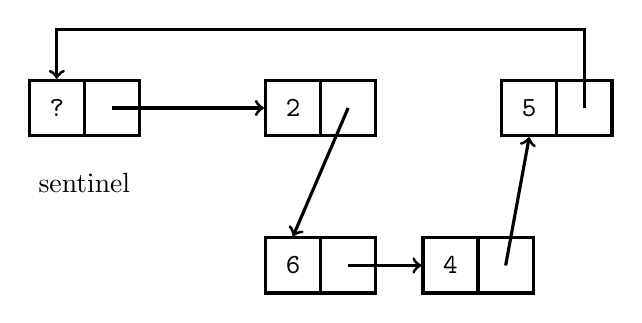
\begin{tikzpicture}

\draw (0.35, 0.35)
  node[draw, line width=0.04cm, , color=black,
       rounded corners=0cm, inner sep=0cm] {

\begin{minipage}[t][0.7cm]{0.7cm}
\mbox{}

\end{minipage}

};\draw (0.35, 0.35) node[color=black] {{\texttt{2}}};
\draw (1.0499999999999998, 0.35)
  node[draw, line width=0.04cm, , color=black,
       rounded corners=0cm, inner sep=0cm] {

\begin{minipage}[t][0.7cm]{0.7cm}
\mbox{}

\end{minipage}

};\draw (1.0499999999999998, 0.35) node[color=black] {{\texttt{}}};
\draw (0.35, -1.65)
  node[draw, line width=0.04cm, , color=black,
       rounded corners=0cm, inner sep=0cm] {

\begin{minipage}[t][0.7cm]{0.7cm}
\mbox{}

\end{minipage}

};\draw (0.35, -1.65) node[color=black] {{\texttt{6}}};
\draw (1.0499999999999998, -1.65)
  node[draw, line width=0.04cm, , color=black,
       rounded corners=0cm, inner sep=0cm] {

\begin{minipage}[t][0.7cm]{0.7cm}
\mbox{}

\end{minipage}

};\draw (1.0499999999999998, -1.65) node[color=black] {{\texttt{}}};
\draw (2.35, -1.65)
  node[draw, line width=0.04cm, , color=black,
       rounded corners=0cm, inner sep=0cm] {

\begin{minipage}[t][0.7cm]{0.7cm}
\mbox{}

\end{minipage}

};\draw (2.35, -1.65) node[color=black] {{\texttt{4}}};
\draw (3.0500000000000003, -1.65)
  node[draw, line width=0.04cm, , color=black,
       rounded corners=0cm, inner sep=0cm] {

\begin{minipage}[t][0.7cm]{0.7cm}
\mbox{}

\end{minipage}

};\draw (3.0500000000000003, -1.65) node[color=black] {{\texttt{}}};
\draw (3.35, 0.35)
  node[draw, line width=0.04cm, , color=black,
       rounded corners=0cm, inner sep=0cm] {

\begin{minipage}[t][0.7cm]{0.7cm}
\mbox{}

\end{minipage}

};\draw (3.35, 0.35) node[color=black] {{\texttt{5}}};
\draw (4.05, 0.35)
  node[draw, line width=0.04cm, , color=black,
       rounded corners=0cm, inner sep=0cm] {

\begin{minipage}[t][0.7cm]{0.7cm}
\mbox{}

\end{minipage}

};\draw (4.05, 0.35) node[color=black] {{\texttt{}}};
\draw (-2.65, 0.35)
  node[draw, line width=0.04cm, , color=black,
       rounded corners=0cm, inner sep=0cm] {

\begin{minipage}[t][0.7cm]{0.7cm}
\mbox{}

\end{minipage}

};\draw (-2.65, 0.35) node[color=black] {{\texttt{?}}};
\draw (-1.9499999999999997, 0.35)
  node[draw, line width=0.04cm, , color=black,
       rounded corners=0cm, inner sep=0cm] {

\begin{minipage}[t][0.7cm]{0.7cm}
\mbox{}

\end{minipage}

};\draw (-1.9499999999999997, 0.35) node[color=black] {{\texttt{}}};\draw[line width=0.04cm,black,->] (-1.95,0.35) to  (-0.02,0.35);
\draw[line width=0.04cm,black,->] (1.05,0.35) to  (0.35,-1.28);
\draw[line width=0.04cm,black,->] (1.05,-1.65) to  (1.98,-1.65);
\draw[line width=0.04cm,black,->] (3.05,-1.65) to  (3.35,-0.02);
\draw[line width=0.04cm,black,->] (4.05,0.35) to  (4.05,1.35) to  (-2.65,1.35) to  (-2.65,0.72);

\draw (-2.3, -0.6)
  node[draw=none, line width=0cm, , color=black,
       rounded corners=0cm, inner sep=0cm] {

\begin{minipage}[t][0.1cm]{0.1cm}
\mbox{}

\end{minipage}

};\draw (-2.3, -0.6) node[color=black] {sentinel};
\end{tikzpicture}

\end{center}



suppose \texttt{10} is decreased to \texttt{1}:

\begin{center}
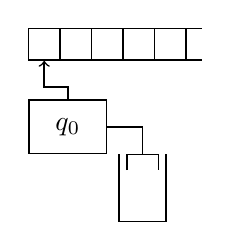
\begin{tikzpicture}

\draw (0.2, 0.2)
  node[draw, line width=0.02cm, , color=black,
       rounded corners=0cm, inner sep=0cm] {

\begin{minipage}[t][0.4cm]{0.4cm}
\mbox{}

\end{minipage}

};\draw (0.2, 0.2) node[color=black] {{\vphantom{\SPACE\SPACE\SPACE\SPACE\SPACE}\texttt{\SPACE}}};
\draw (0.6000000000000001, 0.2)
  node[draw, line width=0.02cm, , color=black,
       rounded corners=0cm, inner sep=0cm] {

\begin{minipage}[t][0.4cm]{0.4cm}
\mbox{}

\end{minipage}

};\draw (0.6000000000000001, 0.2) node[color=black] {{\vphantom{\SPACE\SPACE\SPACE\SPACE\SPACE}\texttt{\SPACE}}};
\draw (1.0, 0.2)
  node[draw, line width=0.02cm, , color=black,
       rounded corners=0cm, inner sep=0cm] {

\begin{minipage}[t][0.4cm]{0.4cm}
\mbox{}

\end{minipage}

};\draw (1.0, 0.2) node[color=black] {{\vphantom{\SPACE\SPACE\SPACE\SPACE\SPACE}\texttt{\SPACE}}};
\draw (1.4000000000000001, 0.2)
  node[draw, line width=0.02cm, , color=black,
       rounded corners=0cm, inner sep=0cm] {

\begin{minipage}[t][0.4cm]{0.4cm}
\mbox{}

\end{minipage}

};\draw (1.4000000000000001, 0.2) node[color=black] {{\vphantom{\SPACE\SPACE\SPACE\SPACE\SPACE}\texttt{\SPACE}}};
\draw (1.7999999999999998, 0.2)
  node[draw, line width=0.02cm, , color=black,
       rounded corners=0cm, inner sep=0cm] {

\begin{minipage}[t][0.4cm]{0.4cm}
\mbox{}

\end{minipage}

};\draw (1.7999999999999998, 0.2) node[color=black] {{\vphantom{\SPACE\SPACE\SPACE\SPACE\SPACE}\texttt{\SPACE}}};\draw[line width=0.02cm,black] (2.0,0.4) to  (2.2,0.4);
\draw[line width=0.02cm,black] (2.0,0.0) to  (2.2,0.0);

\draw (0.5, -0.85)
  node[draw, line width=0.02cm, , color=black,
       rounded corners=0cm, inner sep=0cm] {

\begin{minipage}[t][0.68cm]{0.98cm}
\mbox{}

\end{minipage}

};\draw (0.5, -0.85) node[color=black] {$q_0$};\draw[line width=0.02cm,black,->] (0.5,-0.5) to  (0.5,-0.34) to  (0.2,-0.34) to  (0.2,-0.01);

\draw (1.45, -1.7499999999999998)
  node[draw=none, line width=0cm, , color=black,
       rounded corners=0cm, inner sep=0cm] {

\begin{minipage}[t][0.4cm]{0.4cm}
\mbox{}

\end{minipage}

};\draw[line width=0.02cm,black] (1.15,-1.2) to  (1.15,-2.05) to  (1.75,-2.05) to  (1.75,-1.2);
\draw[line width=0.02cm,black] (1,-0.85) to  (1.45,-0.85) to  (1.45,-1.2);
\draw[line width=0.02cm,black] (1.25,-1.4) to  (1.25,-1.2) to  (1.65,-1.2) to  (1.65,-1.4);
\end{tikzpicture}

\end{center}



Of course this is not a maxheap anymore.
To make this back to a maxheap, clearly the simplest thing to do is
to heapify-down.
In this case I need two swaps.
First I do this swap

\begin{center}
\begin{tikzpicture}

\fill[white] (11.0, 0.0) circle (0.3);
\node [line width=0.03cm,black,minimum size=0.57cm,draw,circle] at (11.0,0.0)(A){};\draw (11.0, 0.0) node[color=black] {\texttt{20}};
\fill[white] (10.0, -0.7) circle (0.3);
\node [line width=0.03cm,black,minimum size=0.57cm,draw,circle] at (10.0,-0.7)(a){};\draw (10.0, -0.7) node[color=black] {\texttt{10}};
\fill[white] (9.0, -1.4) circle (0.3);
\node [line width=0.03cm,black,minimum size=0.57cm,draw,circle] at (9.0,-1.4)(b){};\draw (9.0, -1.4) node[color=black] {\texttt{5}};
\fill[white] (10.0, -2.1) circle (0.3);
\node [line width=0.03cm,black,minimum size=0.57cm,draw,circle] at (10.0,-2.1)(e){};\draw (10.0, -2.1) node[color=black] {\texttt{8}};
\fill[white] (9.0, -2.8) circle (0.3);
\node [line width=0.03cm,black,minimum size=0.57cm,draw,circle] at (9.0,-2.8)(k){};\draw (9.0, -2.8) node[color=black] {\texttt{6}};
\fill[white] (11.0, -2.8) circle (0.3);
\node [line width=0.03cm,black,minimum size=0.57cm,draw,circle] at (11.0,-2.8)(l){};\draw (11.0, -2.8) node[color=black] {\texttt{9}};
\fill[white] (11.0, -1.4) circle (0.3);
\node [line width=0.03cm,black,minimum size=0.57cm,draw,circle] at (11.0,-1.4)(p){};\draw (11.0, -1.4) node[color=black] {\texttt{15}};\draw[line width=0.03cm,black,->,>=triangle 60] (A) to  (a);
\draw[line width=0.03cm,black,->,>=triangle 60] (a) to  (p);
\draw[line width=0.03cm,black,->,>=triangle 60] (a) to  (b);
\draw[line width=0.03cm,black,->,>=triangle 60] (b) to  (e);
\draw[line width=0.03cm,black,->,>=triangle 60] (e) to  (k);
\draw[line width=0.03cm,black,->,>=triangle 60] (e) to  (l);
\end{tikzpicture}

\end{center}



to get this:

\input{stdout53.tex}

Next I do this swap 

\input{stdout54.tex}

to get this:

\begin{center}
\begin{tikzpicture}

\fill[white] (20.0, -2.0) circle (0.3);
\node [line width=0.03cm,black,minimum size=0.57cm,draw,circle] at (20.0,-2.0)(A){};\draw (20.0, -2.0) node[color=black] {\texttt{20}};
\fill[white] (14.0, 0.0) circle (0.3);
\node [line width=0.03cm,black,minimum size=0.57cm,draw,circle] at (14.0,0.0)(a){};\draw (14.0, 0.0) node[color=black] {\texttt{10}};
\fill[white] (10.0, -1.0) circle (0.3);
\node [line width=0.03cm,black,minimum size=0.57cm,draw,circle] at (10.0,-1.0)(b){};\draw (10.0, -1.0) node[color=black] {\texttt{4}};
\fill[white] (18.0, -1.0) circle (0.3);
\node [line width=0.03cm,black,minimum size=0.57cm,draw,circle] at (18.0,-1.0)(p){};\draw (18.0, -1.0) node[color=black] {\texttt{18}};
\fill[white] (8.0, -2.0) circle (0.3);
\node [line width=0.03cm,black,minimum size=0.57cm,draw,circle] at (8.0,-2.0)(e){};\draw (8.0, -2.0) node[color=black] {\texttt{2}};
\fill[white] (7.0, -3.0) circle (0.3);
\node [line width=0.03cm,black,minimum size=0.57cm,draw,circle] at (7.0,-3.0)(k){};\draw (7.0, -3.0) node[color=black] {\texttt{0}};
\fill[white] (9.0, -3.0) circle (0.3);
\node [line width=0.03cm,black,minimum size=0.57cm,draw,circle] at (9.0,-3.0)(l){};\draw (9.0, -3.0) node[color=black] {\texttt{3}};
\fill[white] (16.0, -2.0) circle (0.3);
\node [line width=0.03cm,black,minimum size=0.57cm,draw,circle] at (16.0,-2.0)(h){};\draw (16.0, -2.0) node[color=black] {\texttt{15}};
\fill[white] (15.0, -3.0) circle (0.3);
\node [line width=0.03cm,black,minimum size=0.57cm,draw,circle] at (15.0,-3.0)(m){};\draw (15.0, -3.0) node[color=black] {\texttt{12}};
\fill[white] (12.0, -2.0) circle (0.3);
\node [line width=0.03cm,black,minimum size=0.57cm,draw,circle] at (12.0,-2.0)(f){};\draw (12.0, -2.0) node[color=black] {\texttt{8}};
\fill[white] (11.0, -3.0) circle (0.3);
\node [line width=0.03cm,black,minimum size=0.57cm,draw,circle] at (11.0,-3.0)(n){};\draw (11.0, -3.0) node[color=black] {\texttt{6}};
\fill[white] (13.0, -3.0) circle (0.3);
\node [line width=0.03cm,black,minimum size=0.57cm,draw,circle] at (13.0,-3.0)(o){};\draw (13.0, -3.0) node[color=black] {\texttt{9}};
\fill[white] (17.0, -3.0) circle (0.3);
\node [line width=0.03cm,black,minimum size=0.57cm,draw,circle] at (17.0,-3.0)(q){};\draw (17.0, -3.0) node[color=black] {\texttt{17}};
\fill[white] (19.0, -3.0) circle (0.3);
\node [line width=0.03cm,black,minimum size=0.57cm,draw,circle] at (19.0,-3.0)(r){};\draw (19.0, -3.0) node[color=black] {\texttt{19}};
\fill[white] (21.0, -3.0) circle (0.3);
\node [line width=0.03cm,black,minimum size=0.57cm,draw,circle] at (21.0,-3.0)(s){};\draw (21.0, -3.0) node[color=black] {\texttt{22}};\draw[line width=0.03cm,black,->,>=triangle 60] (a) to  (p);
\draw[line width=0.03cm,black,->,>=triangle 60] (h) to  (m);
\draw[line width=0.03cm,black,->,>=triangle 60] (a) to  (b);
\draw[line width=0.03cm,black,->,>=triangle 60] (p) to  (h);
\draw[line width=0.03cm,black,->,>=triangle 60] (p) to  (A);
\draw[line width=0.03cm,black,->,>=triangle 60] (A) to  (r);
\draw[line width=0.03cm,black,->,>=triangle 60] (A) to  (s);
\draw[line width=0.03cm,black,->,>=triangle 60] (b) to  (e);
\draw[line width=0.03cm,black,->,>=triangle 60] (b) to  (f);
\draw[line width=0.03cm,black,->,>=triangle 60] (e) to  (k);
\draw[line width=0.03cm,black,->,>=triangle 60] (e) to  (l);
\draw[line width=0.03cm,black,->,>=triangle 60] (f) to  (o);
\draw[line width=0.03cm,black,->,>=triangle 60] (h) to  (q);
\draw[line width=0.03cm,black,->,>=triangle 60] (f) to  (n);
\end{tikzpicture}

\end{center}



Here's decrease key:

\begin{Verbatim}[frame=single]
ALGORITHM: decrease_key (for maxheap)
INPUT: x - heap (using an array)
       n - length of heap in x
       i - index where key will increase
       k - new key value (k < x[i])

x[i] = k # originally x[i] > k
Perform heapify_down on x at starting at index i.
\end{Verbatim}

The worse runtime of decrease-key for maxheap is clearly
\[
O(\log n)
\]

It's clear that given a heap (max or min), 
you can heapify-up and heapify-down.
I prefer to use 
\lq\lq heapify-up"
and 
\lq\lq heapify-down"
because the important thing is whether a node moves up or down.
In the case of maxheap, 
heapify-up and heapify-down
are respectively
increase-key and decrease-key
whereas
in the case of minheap
heapify-up and heapify-down
are respectively
decrease-key and increase-key.




\newpage
\begin{ex}
Let $x$ be the array
\[
4, 9, 2, 6, 3, 8, 0, 1, 5, 7
\]
First heapify it.
Next do the following:
\begin{tightlist}
  \item Perform increase-key from on the key with value \texttt{2}
  and change it to \texttt{11}.
  \item Perform decrease-key from on the key with value
  \texttt{7} and change it to \texttt{-1}.
\end{tightlist}
\qed
\end{ex}



\newpage
\begin{ex}
Continuing the implementation of the heap ADT using functions,
implement the increase-key and decrease-key
functions:
\begin{console}
int x;
std::vector< int > heap;

heap.resize(5);
heap[0] = 5;
heap[1] = 7;
heap[2] = 8;
heap[3] = 10;
heap[4] = 2;
maxheap_build(heap);      // [10, 7, 8, 5, 2]

maxheap_increasekey(heap, 2, 12); // heap[2] is changed
                          // to 12. heap has to be
                          // reorganized to become
                          // maxheap again.
                          
maxheap_decreasekey(heap, 2, 0); // heap[2] is changed
                          // to 0. heap has to be
                          // reorganized to become
                          // maxheap again.
\end{console}
\end{ex}

\newpage%-*-latex-*-
\section{Build heap}

Frequently, you want to make an array into a heap.
This is called
\defterm{build-maxheap}\tinysidebar{build-maxheap \\ build-minheap \\ build-heap \\ max-heapify \\ min-heapify \\ heapify}
(if you want to make
the array into a maxheap)
or otherwise it's called
\defterm{build-minheap}.
I'll just call it \defterm{build-heap}
if the type of heap is clear from the context.
It's also called
\defterm{max-heapify}
or
\defterm{min-heapify}
or
\defterm{heapify} (if the context is clear).


\subsection{Slow method}

We can use the heaps to sort arrays.
For instance suppose you have an array
\verb!x! of 10 values.
Looking just at the first value, \verb!x[0]!,
you have a heap of one
value.
Now insert \verb!x[1]! into the heap with only
\verb!x[0]!.
At this point \verb!x[0..1]! is a heap --
say we want to sort it in 
ascending order, which means that we're using maxheap
(you see why later).
Now we repeat to get \verb!x[0..2]! to be a maxheap.
Etc.
When we're done, we have a maxheap of \verb!x[0..9]!.
Inserting into a heap requires $\log_2 n$ steps
where $n$ is the
size of the heap.
Therefore the 
runtime to create the heap 
from an array of $n$ values is, informally speaking, 
$\log_2 1 + \log_2 2 + \cdots + \log_2 n$
which is $\log_2 n! \leq \log_2 n^n = n \log_2 n$.
There's a faster algorithm ... the real build-heap.




\subsection{Fast and right method}

Now for the real build-heap or build-maxheap or build-minheap.

As mentioned at the beginning of this section,
you can create the maxheap by continually inserting values into the
the maxheap.
The runtime is $O(n \log n)$.
Instead of doing that you can
also execute heapify-down on all the non-leaves positions
of the given array is a systematic way: from the non-leaf at the
lowest level to the root, more or less the opposite of the
breadth-first traversal (ignoring the leaves).

Note that if the size of the array is $n$,
then the indices of the leaves are
$n/2$ (integer division), $n/2 + 1$, ..., $n - 1$.
Therefore you can convert the array to a maxheap
if you perform heapify-down at indices
$n/2, n/2-1, n/2-2,...,0$, you will get a maxheap too.

The runtime of build-heap is
\[
  \lg (n/2) + \lg (n/2 + 1) + \cdots + \lg n
\]
Each of these terms are $\leq \lg n$ and there are $n/2$
such heapify operations.
So the runtime is at most $(n/2) \lg n = O(n \lg n)$.
But that's an over-approximation.
It can be shown that the runtime is actually
\[
O(n)
\]
which is faster than the earlier build max heap algorithm
at the beginning of this section.
However this does not improve the overall heapsort
since the second part of the heapsort process will still run
in $O(n \log n)$.

\begin{console}
ALGORITHM: build_maxheap (or heapify)
INPUT: x - array containing n values x[0..n-1] that will
           represent a maxheap at the end of this
           algorithm.
       n - length of x

Perform heapify bottom-up from the first nonleaf to the
root, i.e.,

for i = n/2, n/2 - 1, n/2 - 2, ..., 0:
    perform heapify-down on x at i
\end{console}

As mentioned at the beginning of this section, the runtime of
this build-maxheap has runtime
\[
O(n)
\]

Let me show you how to 
build a maxheap given an array.
Let's say we're given this array:
\[
1, 0, 9, 8, 3, 2, 4, 7, 6
\]
Here's the array drawn as a complete tree:

\begin{python}
from latextool_basic import *
p = Plot()
xs = [1, 0, 9, 8, 3, 2, 4, 7, 6]
edges = array_to_edges(xs)
drawheap(p, edges, include_array=False)

print(p)
\end{python}

The main idea of build-maxheap
is to maintain a collection of subheaps.
Each leaf is already a heap.
So I actually start with 5 subheaps:

\begin{python}
from latextool_basic import *
p = Plot()
xs = [1, 0, 9, 8, 3, 2, 4, 7, 6]
edges = array_to_edges(xs)
drawheap(p, edges, include_array=False)

p += r'\node [ellipse, draw=red, fit=(3), line width=0.1cm, inner sep=0.0cm] {};'
p += r'\node [ellipse, draw=red, fit=(2), line width=0.1cm, inner sep=0.0cm] {};'
p += r'\node [ellipse, draw=red, fit=(4), line width=0.1cm, inner sep=0.0cm] {};'
p += r'\node [ellipse, draw=red, fit=(7), line width=0.1cm, inner sep=0.0cm] {};'
p += r'\node [ellipse, draw=red, fit=(6), line width=0.1cm, inner sep=0.0cm] {};'

print(p)
\end{python}

I now heapify in this order: 8,9,0,1.
By this I mean \verb!8! (at index 3) is going to start off at the
root postion of the heap that combines two subheaps at 7 and 6.


\textsc{Step 1.}
I heapify-down at \texttt{8} (at index 3).
There's no change since the
subtree at \texttt{8} is a maxheap.

\begin{python}
from latextool_basic import *
p = Plot()
xs = [1, 0, 9, 8, 3, 2, 4, 7, 6]
edges = array_to_edges(xs)
drawheap(p, edges, include_array=False)

p += r'\node [ellipse, draw=red, fit=(3), line width=0.1cm, inner sep=0.0cm] {};'
p += r'\node [ellipse, draw=red, fit=(2), line width=0.1cm, inner sep=0.0cm] {};'
p += r'\node [ellipse, draw=red, fit=(4), line width=0.1cm, inner sep=0.0cm] {};'
p += r'\node [ellipse, draw=red, fit=(8) (7) (6), line width=0.1cm, inner sep=0.0cm] {};'

print(p)
\end{python}


\textsc{Step 2.}
Heapify-down at index 2 with value \texttt{9}:
No change since the subtree at \texttt{9} is a maxheap.

\begin{python}
from latextool_basic import *
p = Plot()
xs = [1, 0, 9, 8, 3, 2, 4, 7, 6]
edges = array_to_edges(xs)
drawheap(p, edges,
    include_array=False)

p += r'\node [ellipse, draw=red, fit=(3), line width=0.1cm, inner sep=0.0cm] {};'
p += r'\node [ellipse, draw=red, fit=(9) (2) (4), line width=0.1cm, inner sep=0.0cm] {};'
p += r'\node [ellipse, draw=red, fit=(8) (7) (6), line width=0.1cm, inner sep=0.0cm] {};'

print(p)
\end{python}


\textsc{Step 3.}
Heapify-down at index 1 with value \texttt{0}:
I need 2 swaps.
After that the subtree at position where \texttt{0} originally 
was a maxheap.

\begin{python}
from latextool_basic import *
p = Plot()
xs = [1, 8, 9, 7, 3, 2, 4, 0, 6]
edges = array_to_edges(xs)
drawheap(p, edges,
    include_array=False)

p += r'\node [ellipse, draw=red, fit=(9) (2) (4), line width=0.1cm, inner sep=0.0cm] {};'
p += r'\node [ellipse, draw=red, fit=(3) (0) (8) (7) (6), line width=0.1cm, inner sep=0.0cm] {};'

print(p)
\end{python}

\textsc{Step 4.}
Heapify-down at index 0 with value \texttt{1}:
I need 2 swaps.
After that the subtree at the place
where \texttt{1} was is a maxheap.

\begin{python}
from latextool_basic import *
p = Plot()
xs = [9, 8, 4, 7, 3, 2, 1, 0, 6]
edges = array_to_edges(xs)
drawheap(p, edges, include_array=False)

p += r'\node [ellipse, draw=red, fit=(9) (8) (4) (7) (3) (2) (1) (0) (6), line width=0.1cm, inner sep=0.0cm] {};'

print(p)
\end{python}

I'm done!

Hence I get this array (which represents the above maxheap):
\[
9,8,4,7,3,2,1,0,6
\]


\newpage
\begin{ex}
Draw the corresponding array at the end of each stage
for the above computation
\qed
\end{ex}


\newpage
\begin{ex}
Perform build-maxheap on the following array:
\[
5,3,0,7,1,2,6,9,4,8
\]
showing every step (like in the above example).
\qed
\end{ex}


\newpage
\begin{ex}
Perform build-maxheap on the following array:
\[
2,1,5,0,3,7,9,6,4,8
\]
showing every step (like in the above example).
\qed
\end{ex}


\newpage
\begin{ex}
Perform build-maxheap on the following array:
\[
0,1,2,3,4,5,6,7,8,9
\]
showing every step (like in the above example).
\qed
\end{ex}



\newpage%-*-latex-*-
% https://en.wikipedia.org/wiki/Heapsort#Variations

\sectionthree{Heapsort}
\begin{python0}
from solutions import *; clear()
\end{python0}

\textsc{Heapsort given a maxheap.}
Now we delete the root from the heap.
Because this is a maxheap, the root, is the 
maximum value of \verb!x[0..9]!.
We swap \verb!x[0]! and \verb!x[9]!
and re-heapify to get a heap \verb!x[0..8]!.
In other words we're essentially doing a delete of the value at \verb!x[0]!
(the extract-max operation), putting this value at \texttt{x[9]}.

We repeat the above to get a heap \verb!x[0..7]!.
At this point the largest value of the array is at \verb!x[9]!
and the second largest is at \verb!x[8]!.

We repeat until the heap has only one value, i.e., the heap is \verb!x[0]!.
The whole array must be sorted in ascending order.

The runtime is, informally, $\log_2 n + \log_2 (n - 1) + \cdots$
which is $\log_2 n! \leq \log_2 n^n = n \log_2 n$.

So the total time for the above process,
creating the heap and then removing roots from the 
heap is roughly $2 n \log_2 n$ and therefore
the runtime for heapsort is $O(n \log_2 n)$.

Note that the heapsort has a worse runtime of $n \log_2 n$
whereas quicksort can have a worse runtime of $n^2$
although
on the average quicksort is $O(n \log n)$ and 
typically quicksort is faster than heapsort by a constant
factor.
Although mergesort does achieve $n \log_2 n$ for worse runtime,
remember that mergesort needs $O(n)$ space.
However heapsort is not stable whereas mergesort is stable.

\begin{ex}
  Give an example showing that heapsort is not
  stable.
\end{ex}
  
  

\newpage
Here is a maxheap say constructed
using build-maxheap:


\begin{center}

\begin{tikzpicture}
\node at (4,-0.8) [minimum size=8mm] (Z) {$$};
\node at (2,-1.6) [circle,draw,minimum size=8mm] (A) {$\beta$};
\node at (0,-2.4000000000000004)
    [isosceles triangle, shape border rotate=+90,
     draw,minimum size=8mm,minimum height=2cm,
     anchor=north] (Ctriangle) {$T_1$};
\coordinate (C) at (0,-2.4000000000000004);
\node at (4,-2.4000000000000004) [circle,draw,minimum size=8mm] (B) {$\alpha$};
\node at (3,-3.2)
    [isosceles triangle, shape border rotate=+90,
     draw,minimum size=8mm,minimum height=2cm,
     anchor=north] (Dtriangle) {$T_2$};
\coordinate (D) at (3,-3.2);
\node at (5,-3.2)
    [isosceles triangle, shape border rotate=+90,
     draw,minimum size=8mm,minimum height=2cm,
     anchor=north] (Etriangle) {$T_3$};
\coordinate (E) at (5,-3.2);
\draw [-,thick] (Z) -- (A);
\draw [-,thick] (A) -- (B);
\draw [-,thick] (A) -- (C);
\draw [-,thick] (B) -- (D);
\draw [-,thick] (B) -- (E);

;
\end{tikzpicture}
    
\end{center}


Let's perform heapsort on this maxheap.
Recall that extract-root will throw away the root by replacing
the value at the root with the last value in the tree (i.e.,
the rightmost value at the last level of the tree).
Instead of replacing the root with the last value,
I will \textit{swap} the root value and last value.
Otherwise it's the same extract-root operation.
Let's do it.


\textsc{Step 1}.
First I swap the root value and the last value:

\include{stdout63.tex}

x,y = pos[9]; p += Graph.node(x=x, y=y, r=BinTree.node_width, background='red!10', label='9')
p += Graph.edge(names=[7,9], linecolor='white', linewidth=0.1)
p += Graph.edge(names=[7,9], linestyle='dashed')

print(p)

I color \texttt{9} in red to remind myself
that the \texttt{9} should not be considered part of the maxheap,
but of course it's in the array.
In terms of an array the above diagram would correspond to this array:

\begin{center}
\begin{tikzpicture}

\fill[white] (5.0, 0.0) circle (0.3);
\node [draw=none,line width=0cm,black,minimum size=0.6cm,circle] at (5.0,0.0)(X){};
\fill[white] (17.0, 0.0) circle (0.3);
\node [draw=none,line width=0cm,black,minimum size=0.6cm,circle] at (17.0,0.0)(Y){};
\fill[white] (11.0, 0.0) circle (0.3);
\node [line width=0.03cm,black,minimum size=0.57cm,draw,circle] at (11.0,0.0)(a){};\draw (11.0, 0.0) node[color=black] {\texttt{18}};
\fill[white] (9.0, -1.0) circle (0.3);
\node [line width=0.03cm,black,minimum size=0.57cm,draw,circle] at (9.0,-1.0)(b){};\draw (9.0, -1.0) node[color=black] {\texttt{10}};
\fill[white] (14.0, -2.0) circle (0.3);
\node [line width=0.03cm,black,minimum size=0.57cm,draw,circle] at (14.0,-2.0)(d){};\draw (14.0, -2.0) node[color=black] {\texttt{20}};
\fill[white] (8.0, -2.0) circle (0.3);
\node [line width=0.03cm,black,minimum size=0.57cm,draw,circle] at (8.0,-2.0)(e){};\draw (8.0, -2.0) node[color=black] {\texttt{4}};
\fill[white] (12.0, -2.0) circle (0.3);
\node [line width=0.03cm,black,minimum size=0.57cm,draw,circle] at (12.0,-2.0)(f){};\draw (12.0, -2.0) node[color=black] {\texttt{19}};
\fill[white] (8.0, -4.0) circle (0.3);
\node [line width=0.03cm,black,minimum size=0.57cm,draw,circle] at (8.0,-4.0)(k){};\draw (8.0, -4.0) node[color=black] {\texttt{3}};
\fill[white] (7.0, -3.0) circle (0.3);
\node [line width=0.03cm,black,minimum size=0.57cm,draw,circle] at (7.0,-3.0)(l){};\draw (7.0, -3.0) node[color=black] {\texttt{2}};
\fill[white] (13.0, -1.0) circle (0.3);
\node [line width=0.03cm,black,minimum size=0.57cm,draw,circle] at (13.0,-1.0)(p){};\draw (13.0, -1.0) node[color=black] {\texttt{26}};
\fill[white] (6.0, -4.0) circle (0.3);
\node [line width=0.03cm,black,minimum size=0.57cm,draw,circle] at (6.0,-4.0)(n){};\draw (6.0, -4.0) node[color=black] {\texttt{0}};
\fill[white] (10.0, -2.0) circle (0.3);
\node [line width=0.03cm,black,minimum size=0.57cm,draw,circle] at (10.0,-2.0)(q){};\draw (10.0, -2.0) node[color=black] {\texttt{17}};\draw[line width=0.03cm,black,->,>=triangle 60] (e) to  (l);
\draw[line width=0.03cm,black,->,>=triangle 60] (p) to  (d);
\draw[line width=0.03cm,black,->,>=triangle 60] (b) to  (q);
\draw[line width=0.03cm,black,->,>=triangle 60] (l) to  (n);
\draw[line width=0.03cm,black,->,>=triangle 60] (l) to  (k);
\draw[line width=0.03cm,black,->,>=triangle 60] (p) to  (f);
\draw[line width=0.03cm,black,->,>=triangle 60] (a) to  (p);
\draw[line width=0.03cm,black,->,>=triangle 60] (a) to  (b);
\draw[line width=0.03cm,black,->,>=triangle 60] (b) to  (e);
\end{tikzpicture}

\end{center}



I still need to heapify-down the \texttt{6} to get this:

\begin{center}
\begin{tikzpicture}

\fill[white] (5.0, 0.0) circle (0.3);
\node [draw=none,line width=0cm,black,minimum size=0.6cm,circle] at (5.0,0.0)(X){};
\fill[white] (17.0, 0.0) circle (0.3);
\node [draw=none,line width=0cm,black,minimum size=0.6cm,circle] at (17.0,0.0)(Y){};
\fill[white] (13.0, -1.0) circle (0.3);
\node [line width=0.03cm,black,minimum size=0.57cm,draw,circle] at (13.0,-1.0)(a){};\draw (13.0, -1.0) node[color=black] {\texttt{10}};
\fill[white] (11.0, 0.0) circle (0.3);
\node [line width=0.03cm,black,minimum size=0.57cm,draw,circle] at (11.0,0.0)(b){};\draw (11.0, 0.0) node[color=black] {\texttt{4}};
\fill[white] (15.0, -3.0) circle (0.3);
\node [line width=0.03cm,black,minimum size=0.57cm,draw,circle] at (15.0,-3.0)(d){};\draw (15.0, -3.0) node[color=black] {\texttt{20}};
\fill[white] (9.0, -1.0) circle (0.3);
\node [line width=0.03cm,black,minimum size=0.57cm,draw,circle] at (9.0,-1.0)(e){};\draw (9.0, -1.0) node[color=black] {\texttt{2}};
\fill[white] (13.0, -3.0) circle (0.3);
\node [line width=0.03cm,black,minimum size=0.57cm,draw,circle] at (13.0,-3.0)(f){};\draw (13.0, -3.0) node[color=black] {\texttt{17}};
\fill[white] (8.0, -2.0) circle (0.3);
\node [line width=0.03cm,black,minimum size=0.57cm,draw,circle] at (8.0,-2.0)(k){};\draw (8.0, -2.0) node[color=black] {\texttt{0}};
\fill[white] (10.0, -2.0) circle (0.3);
\node [line width=0.03cm,black,minimum size=0.57cm,draw,circle] at (10.0,-2.0)(l){};\draw (10.0, -2.0) node[color=black] {\texttt{3}};
\fill[white] (14.0, -2.0) circle (0.3);
\node [line width=0.03cm,black,minimum size=0.57cm,draw,circle] at (14.0,-2.0)(p){};\draw (14.0, -2.0) node[color=black] {\texttt{18}};
\fill[white] (14.0, -4.0) circle (0.3);
\node [line width=0.03cm,black,minimum size=0.57cm,draw,circle] at (14.0,-4.0)(h){};\draw (14.0, -4.0) node[color=black] {\texttt{19}};
\fill[white] (16.0, -4.0) circle (0.3);
\node [line width=0.03cm,black,minimum size=0.57cm,draw,circle] at (16.0,-4.0)(m){};\draw (16.0, -4.0) node[color=black] {\texttt{26}};\draw[line width=0.03cm,black,->,>=triangle 60] (b) to  (a);
\draw[line width=0.03cm,black,->,>=triangle 60] (p) to  (f);
\draw[line width=0.03cm,black,->,>=triangle 60] (p) to  (d);
\draw[line width=0.03cm,black,->,>=triangle 60] (a) to  (p);
\draw[line width=0.03cm,black,->,>=triangle 60] (b) to  (e);
\draw[line width=0.03cm,black,->,>=triangle 60] (e) to  (k);
\draw[line width=0.03cm,black,->,>=triangle 60] (e) to  (l);
\draw[line width=0.03cm,black,->,>=triangle 60] (d) to  (h);
\draw[line width=0.03cm,black,->,>=triangle 60] (d) to  (m);
\end{tikzpicture}

\end{center}


\include{stdout66.tex}

Because I started with a maxheap, \verb!9!, the value I get from extract-root,
is the largest value in the array.
Since it moved to the last index position in the array,
this means that \verb!9! has found its right place.


\textsc{Step 2}.
Now I repeat the above process:
first I swap the root (i.e., \texttt{8}) and
the last value of the tree (i.e., \texttt{0}) to get this:


\begin{center}
\begin{tikzpicture}

\fill[white] (0.0, 0.0) circle (0.3);
\node [line width=0.03cm,black,minimum size=0.57cm,draw,circle] at (0.0,0.0)(14){};\draw (0.0, 0.0) node[color=black] {\texttt{14}};
\fill[white] (-3.2, -1.0) circle (0.3);
\node [line width=0.03cm,black,minimum size=0.57cm,draw,circle] at (-3.2,-1.0)(9){};\draw (-3.2, -1.0) node[color=black] {\texttt{9}};
\fill[white] (3.2, -1.0) circle (0.3);
\node [line width=0.03cm,black,minimum size=0.57cm,draw,circle] at (3.2,-1.0)(18){};\draw (3.2, -1.0) node[color=black] {\texttt{18}};
\fill[white] (-4.8, -2.0) circle (0.3);
\node [line width=0.03cm,black,minimum size=0.57cm,draw,circle] at (-4.8,-2.0)(5){};\draw (-4.8, -2.0) node[color=black] {\texttt{5}};
\fill[white] (-1.6, -2.0) circle (0.3);
\node [line width=0.03cm,black,minimum size=0.57cm,draw,circle] at (-1.6,-2.0)(13){};\draw (-1.6, -2.0) node[color=black] {\texttt{13}};
\fill[white] (1.6, -2.0) circle (0.3);
\node [line width=0.03cm,black,minimum size=0.57cm,draw,circle] at (1.6,-2.0)(15){};\draw (1.6, -2.0) node[color=black] {\texttt{15}};
\fill[white] (4.8, -2.0) circle (0.3);
\node [line width=0.03cm,black,minimum size=0.57cm,draw,circle] at (4.8,-2.0)(22){};\draw (4.8, -2.0) node[color=black] {\texttt{22}};
\fill[white] (-5.6, -3.0) circle (0.3);
\node [line width=0.03cm,black,minimum size=0.57cm,draw,circle] at (-5.6,-3.0)(0){};\draw (-5.6, -3.0) node[color=black] {\texttt{0}};
\fill[white] (-4.0, -3.0) circle (0.3);
\node [line width=0.03cm,black,minimum size=0.57cm,draw,circle] at (-4.0,-3.0)(8){};\draw (-4.0, -3.0) node[color=black] {\texttt{8}};
\fill[white] (-2.4, -3.0) circle (0.3);
\node [line width=0.03cm,black,minimum size=0.57cm,draw,circle] at (-2.4,-3.0)(10){};\draw (-2.4, -3.0) node[color=black] {\texttt{10}};
\fill[white] (4.0, -3.0) circle (0.3);
\node [line width=0.03cm,black,minimum size=0.57cm,draw,circle] at (4.0,-3.0)(21){};\draw (4.0, -3.0) node[color=black] {\texttt{21}};
\fill[white] (5.6, -3.0) circle (0.3);
\node [line width=0.03cm,black,minimum size=0.57cm,draw,circle] at (5.6,-3.0)(31){};\draw (5.6, -3.0) node[color=black] {\texttt{31}};
\fill[white] (-4.4, -4.0) circle (0.3);
\node [line width=0.03cm,black,minimum size=0.57cm,draw,circle] at (-4.4,-4.0)(7){};\draw (-4.4, -4.0) node[color=black] {\texttt{7}};
\fill[white] (-2.0, -4.0) circle (0.3);
\node [line width=0.03cm,black,minimum size=0.57cm,draw,circle] at (-2.0,-4.0)(11){};\draw (-2.0, -4.0) node[color=black] {\texttt{11}};
\fill[white] (3.6, -4.0) circle (0.3);
\node [line width=0.03cm,black,minimum size=0.57cm,draw,circle] at (3.6,-4.0)(19){};\draw (3.6, -4.0) node[color=black] {\texttt{19}};\draw[line width=0.03cm,black,->,>=triangle 60] (14) to  (9);
\draw[line width=0.03cm,black,->,>=triangle 60] (14) to  (18);
\draw[line width=0.03cm,black,->,>=triangle 60] (9) to  (5);
\draw[line width=0.03cm,black,->,>=triangle 60] (9) to  (13);
\draw[line width=0.03cm,black,->,>=triangle 60] (18) to  (15);
\draw[line width=0.03cm,black,->,>=triangle 60] (18) to  (22);
\draw[line width=0.03cm,black,->,>=triangle 60] (5) to  (0);
\draw[line width=0.03cm,black,->,>=triangle 60] (5) to  (8);
\draw[line width=0.03cm,black,->,>=triangle 60] (13) to  (10);
\draw[line width=0.03cm,black,->,>=triangle 60] (22) to  (21);
\draw[line width=0.03cm,black,->,>=triangle 60] (22) to  (31);
\draw[line width=0.03cm,black,->,>=triangle 60] (8) to  (7);
\draw[line width=0.03cm,black,->,>=triangle 60] (10) to  (11);
\draw[line width=0.03cm,black,->,>=triangle 60] (21) to  (19);
\end{tikzpicture}

\end{center}


\begin{center}
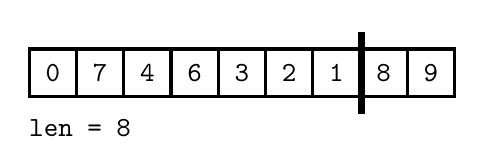
\begin{tikzpicture}

\draw (0.3, -0.3)
  node[draw, line width=0.04cm, , color=black,
       rounded corners=0cm, inner sep=0cm] {

\begin{minipage}[t][0.6cm]{0.6cm}
\mbox{}

\end{minipage}

};\draw (0.3, -0.3) node[color=black] {{\texttt{0}}};
\draw (0.8999999999999999, -0.3)
  node[draw, line width=0.04cm, , color=black,
       rounded corners=0cm, inner sep=0cm] {

\begin{minipage}[t][0.6cm]{0.6cm}
\mbox{}

\end{minipage}

};\draw (0.8999999999999999, -0.3) node[color=black] {{\texttt{7}}};
\draw (1.5, -0.3)
  node[draw, line width=0.04cm, , color=black,
       rounded corners=0cm, inner sep=0cm] {

\begin{minipage}[t][0.6cm]{0.6cm}
\mbox{}

\end{minipage}

};\draw (1.5, -0.3) node[color=black] {{\texttt{4}}};
\draw (2.0999999999999996, -0.3)
  node[draw, line width=0.04cm, , color=black,
       rounded corners=0cm, inner sep=0cm] {

\begin{minipage}[t][0.6cm]{0.6cm}
\mbox{}

\end{minipage}

};\draw (2.0999999999999996, -0.3) node[color=black] {{\texttt{6}}};
\draw (2.7, -0.3)
  node[draw, line width=0.04cm, , color=black,
       rounded corners=0cm, inner sep=0cm] {

\begin{minipage}[t][0.6cm]{0.6cm}
\mbox{}

\end{minipage}

};\draw (2.7, -0.3) node[color=black] {{\texttt{3}}};
\draw (3.3, -0.3)
  node[draw, line width=0.04cm, , color=black,
       rounded corners=0cm, inner sep=0cm] {

\begin{minipage}[t][0.6cm]{0.6cm}
\mbox{}

\end{minipage}

};\draw (3.3, -0.3) node[color=black] {{\texttt{2}}};
\draw (3.9, -0.3)
  node[draw, line width=0.04cm, , color=black,
       rounded corners=0cm, inner sep=0cm] {

\begin{minipage}[t][0.6cm]{0.6cm}
\mbox{}

\end{minipage}

};\draw (3.9, -0.3) node[color=black] {{\texttt{1}}};
\draw (4.5, -0.3)
  node[draw, line width=0.04cm, , color=black,
       rounded corners=0cm, inner sep=0cm] {

\begin{minipage}[t][0.6cm]{0.6cm}
\mbox{}

\end{minipage}

};\draw (4.5, -0.3) node[color=black] {{\texttt{8}}};
\draw (5.1, -0.3)
  node[draw, line width=0.04cm, , color=black,
       rounded corners=0cm, inner sep=0cm] {

\begin{minipage}[t][0.6cm]{0.6cm}
\mbox{}

\end{minipage}

};\draw (5.1, -0.3) node[color=black] {{\texttt{9}}};\draw[line width=0.1cm,black] (4.22,-0.82) to  (4.22,0.22);

\draw (1.0, -1.0)
  node[draw=none, line width=0cm, , color=black,
       rounded corners=0cm, inner sep=0cm] {

\begin{minipage}[t][0.1cm]{2cm}
\mbox{}

\end{minipage}

};
\draw (1.0, -1.0) node[color=black,
 inner sep=0cm] {
 
\begin{minipage}[t][0.1cm]{2cm}
\texttt{len = 8}
\end{minipage}

};
\end{tikzpicture}

\end{center}



(at this point \verb!9! and \verb!8! are not part of the heap)
then I heapify-down \texttt{0} to get this:

\begin{center}
\begin{tikzpicture}

\fill[white] (0.0, 0.0) circle (0.3);
\node [line width=0.03cm,black,minimum size=0.57cm,draw,circle] at (0.0,0.0)(10){};\draw (0.0, 0.0) node[color=black] {\texttt{10}};
\fill[white] (-3.0, -1.0) circle (0.3);
\node [line width=0.03cm,black,minimum size=0.57cm,draw,circle] at (-3.0,-1.0)(2){};\draw (-3.0, -1.0) node[color=black] {\texttt{2}};
\fill[white] (3.0, -1.0) circle (0.3);
\node [line width=0.03cm,black,minimum size=0.57cm,draw,circle] at (3.0,-1.0)(18){};\draw (3.0, -1.0) node[color=black] {\texttt{18}};
\fill[white] (-4.5, -2.0) circle (0.3);
\node [line width=0.03cm,black,minimum size=0.57cm,draw,circle] at (-4.5,-2.0)(0){};\draw (-4.5, -2.0) node[color=black] {\texttt{0}};
\fill[white] (-1.5, -2.0) circle (0.3);
\node [line width=0.03cm,black,minimum size=0.57cm,draw,circle] at (-1.5,-2.0)(4){};\draw (-1.5, -2.0) node[color=black] {\texttt{4}};
\fill[white] (1.5, -2.0) circle (0.3);
\node [line width=0.03cm,black,minimum size=0.57cm,draw,circle] at (1.5,-2.0)(17){};\draw (1.5, -2.0) node[color=black] {\texttt{17}};
\fill[white] (4.5, -2.0) circle (0.3);
\node [line width=0.03cm,black,minimum size=0.57cm,draw,circle] at (4.5,-2.0)(20){};\draw (4.5, -2.0) node[color=black] {\texttt{20}};
\fill[white] (-2.25, -3.0) circle (0.3);
\node [line width=0.03cm,black,minimum size=0.57cm,draw,circle] at (-2.25,-3.0)(3){};\draw (-2.25, -3.0) node[color=black] {\texttt{3}};\draw[line width=0.03cm,black,->,>=triangle 60] (10) to  (2);
\draw[line width=0.03cm,black,->,>=triangle 60] (10) to  (18);
\draw[line width=0.03cm,black,->,>=triangle 60] (4) to  (3);
\draw[line width=0.03cm,black,->,>=triangle 60] (2) to  (0);
\draw[line width=0.03cm,black,->,>=triangle 60] (2) to  (4);
\draw[line width=0.03cm,black,->,>=triangle 60] (18) to  (17);
\draw[line width=0.03cm,black,->,>=triangle 60] (18) to  (20);
\end{tikzpicture}

\end{center}



The array is


\begin{center}

\begin{tikzpicture}
\node at (3,-0.8) [minimum size=8mm] (E) {$$};
\node at (2,-2.4000000000000004) [circle,draw,minimum size=8mm] (A) {$\alpha$};
\node at (0,-3.2)
    [isosceles triangle, shape border rotate=+90,
     draw,minimum size=8mm,minimum height=2cm,
     anchor=north] (Ctriangle) {$T_1$};
\coordinate (C) at (0,-3.2);
\node at (4,-3.2)
    [isosceles triangle, shape border rotate=+90,
     draw,minimum size=8mm,minimum height=2cm,
     anchor=north] (Btriangle) {$T_2$};
\coordinate (B) at (4,-3.2);
\draw [-,thick] (A) -- (B);
\draw [-,thick] (A) -- (C);
\draw [-,thick] (E) -- (A);

;
\end{tikzpicture}
    
\end{center}



This is the second extract-max.
This means that \verb!8! is the second largest value in the array.
Note also that it's in its right place.


\textsc{Step 3}.
Next I swap the root value (i.e., \texttt{7}) and the last value
of the tree (i.e., \texttt{1})

\include{stdout71.tex}
from latextool_basic import *
p = Plot()
xs = [1, 6, 4, 0, 3, 2, 7, 8, 9]
edges = array_to_edges(xs)
pos = drawheap(p, edges, include_array=False)

x,y = pos[9]; p += Graph.node(x=x, y=y, r=BinTree.node_width, background='red!10', label='9')
x,y = pos[8]; p += Graph.node(x=x, y=y, r=BinTree.node_width, background='red!10', label='8')
x,y = pos[7]; p += Graph.node(x=x, y=y, r=BinTree.node_width, background='red!10', label='7')

p += Graph.edge(names=[0,9], linecolor='white', linewidth=0.1); p += Graph.edge(names=[0,9], linestyle='dashed')
p += Graph.edge(names=[0,8], linecolor='white', linewidth=0.1); p += Graph.edge(names=[0,8], linestyle='dashed')
p += Graph.edge(names=[4,7], linecolor='white', linewidth=0.1); p += Graph.edge(names=[4,7], linestyle='dashed')

print(p)

and heapify at \texttt{1} to get this:


\begin{center}

\begin{tikzpicture}
\node at (4,-0.8) [minimum size=8mm] (E) {$$};
\node at (3,-2.4000000000000004) [circle,draw,minimum size=8mm] (A) {$\alpha$};
\node at (1,-3.2) [circle,draw,minimum size=8mm] (C) {$\beta$};
\node at (5,-3.2)
    [isosceles triangle, shape border rotate=+90,
     draw,minimum size=8mm,
     anchor=north] (Btriangle) {$T'_3$};
\coordinate (B) at (5,-3.2);
\node at (0,-4.0)
    [isosceles triangle, shape border rotate=+90,
     draw,minimum size=8mm,
     anchor=north] (Dtriangle) {$T'_1$};
\coordinate (D) at (0,-4.0);
\node at (2,-4.0)
    [isosceles triangle, shape border rotate=+90,
     draw,minimum size=8mm,
     anchor=north] (Ftriangle) {$T'_2$};
\coordinate (F) at (2,-4.0);
\draw [-,thick] (A) -- (B);
\draw [-,thick] (A) -- (C);
\draw [-,thick] (E) -- (A);
\draw [-,thick] (C) -- (D);
\draw [-,thick] (C) -- (F);

;
\end{tikzpicture}
    
\end{center}


from latextool_basic import *
p = Plot()
xs = [6, 3, 4, 0, 1, 2, 7, 8, 9]
edges = array_to_edges(xs)
pos = drawheap(p, edges, include_array=False)

x,y = pos[9]; p += Graph.node(x=x, y=y, r=BinTree.node_width, background='red!10', label='9')
x,y = pos[8]; p += Graph.node(x=x, y=y, r=BinTree.node_width, background='red!10', label='8')
x,y = pos[7]; p += Graph.node(x=x, y=y, r=BinTree.node_width, background='red!10', label='7')

p += Graph.edge(names=[0,9], linecolor='white', linewidth=0.1); p += Graph.edge(names=[0,9], linestyle='dashed')
p += Graph.edge(names=[0,8], linecolor='white', linewidth=0.1); p += Graph.edge(names=[0,8], linestyle='dashed')
p += Graph.edge(names=[4,7], linecolor='white', linewidth=0.1); p += Graph.edge(names=[4,7], linestyle='dashed')

print(p)
\include{stdout73.tex}
from latextool_basic import *
p = Plot()
a = Array2d(0, 0, width=0.6, height=0.6, 
             xs=[['6','3', '4','0','1','2','7','8','9']])
p += a
p0 = a[0][5].bottomright(); p0 = (p0[0], p0[1] - 0.2)
p1 = a[0][5].topright(); p1 = (p1[0], p1[1] + 0.2)
p += Line(points=[p0, p1], linewidth=0.1)
p += Rect(x0=0, y0=-1, x1=2, y1=-1, s=r'\texttt{len = 6}', linewidth=0) 
print(p)

\textsc{Step 4}.
I swap \texttt{6} and \texttt{2}:

\include{stdout74.tex}
from latextool_basic import *
from drawheap import *
p = Plot()
xs = [2, 3, 4, 0, 1, 6, 7, 8, 9]
edges = array_to_edges(xs)
pos = drawheap(p, edges, include_array=False)

x,y = pos[9]; p += Graph.node(x=x, y=y, r=BinTree.node_width, background='red!10', label='9')
x,y = pos[8]; p += Graph.node(x=x, y=y, r=BinTree.node_width, background='red!10', label='8')
x,y = pos[7]; p += Graph.node(x=x, y=y, r=BinTree.node_width, background='red!10', label='7')
x,y = pos[6]; p += Graph.node(x=x, y=y, r=BinTree.node_width, background='red!10', label='6')

p += Graph.edge(names=[0,9], linecolor='white', linewidth=0.1); p += Graph.edge(names=[0,9], linestyle='dashed')
p += Graph.edge(names=[0,8], linecolor='white', linewidth=0.1); p += Graph.edge(names=[0,8], linestyle='dashed')
p += Graph.edge(names=[4,7], linecolor='white', linewidth=0.1); p += Graph.edge(names=[4,7], linestyle='dashed')
p += Graph.edge(names=[4,6], linecolor='white', linewidth=0.1); p += Graph.edge(names=[4,6], linestyle='dashed')

print(p)

and heapify-down at \texttt{2} to get:

\include{stdout75.tex}
from latextool_basic import *
p = Plot()
xs = [4, 3, 2, 0, 1, 6, 7, 8, 9]
edges = array_to_edges(xs)
pos = drawheap(p, edges, include_array=False)

x,y = pos[9]; p += Graph.node(x=x, y=y, r=BinTree.node_width, background='red!10', label='9')
x,y = pos[8]; p += Graph.node(x=x, y=y, r=BinTree.node_width, background='red!10', label='8')
x,y = pos[7]; p += Graph.node(x=x, y=y, r=BinTree.node_width, background='red!10', label='7')
x,y = pos[6]; p += Graph.node(x=x, y=y, r=BinTree.node_width, background='red!10', label='6')

p += Graph.edge(names=[0,9], linecolor='white', linewidth=0.1); p += Graph.edge(names=[0,9], linestyle='dashed')
p += Graph.edge(names=[0,8], linecolor='white', linewidth=0.1); p += Graph.edge(names=[0,8], linestyle='dashed')
p += Graph.edge(names=[2,7], linecolor='white', linewidth=0.1); p += Graph.edge(names=[2,7], linestyle='dashed')
p += Graph.edge(names=[2,6], linecolor='white', linewidth=0.1); p += Graph.edge(names=[2,6], linestyle='dashed')

print(p)
\include{stdout76.tex}
from latextool_basic import *
p = Plot()
a = Array2d(0, 0, width=0.6, height=0.6, 
             xs=[['4','3','2','0','1','6','7','8','9']])
p += a
p0 = a[0][4].bottomright(); p0 = (p0[0], p0[1] - 0.2)
p1 = a[0][4].topright(); p1 = (p1[0], p1[1] + 0.2)
p += Line(points=[p0, p1], linewidth=0.1)
p += Rect(x0=0, y0=-1, x1=2, y1=-1, s=r'\texttt{len = 5}', linewidth=0) 
print(p)


\textsc{Step 5}.
I swap \texttt{4} and \texttt{1}:

\include{stdout77.tex}
from latextool_basic import *
p = Plot()
xs = [1, 3, 2, 0, 4, 6, 7, 8, 9]
edges = array_to_edges(xs)
pos = drawheap(p, edges, include_array=False)

x,y = pos[9]; p += Graph.node(x=x, y=y, r=BinTree.node_width, background='red!10', label='9')
x,y = pos[8]; p += Graph.node(x=x, y=y, r=BinTree.node_width, background='red!10', label='8')
x,y = pos[7]; p += Graph.node(x=x, y=y, r=BinTree.node_width, background='red!10', label='7')
x,y = pos[6]; p += Graph.node(x=x, y=y, r=BinTree.node_width, background='red!10', label='6')
x,y = pos[4]; p += Graph.node(x=x, y=y, r=BinTree.node_width, background='red!10', label='4')

p += Graph.edge(names=[0,9], linecolor='white', linewidth=0.1); p += Graph.edge(names=[0,9], linestyle='dashed')
p += Graph.edge(names=[0,8], linecolor='white', linewidth=0.1); p += Graph.edge(names=[0,8], linestyle='dashed')
p += Graph.edge(names=[2,7], linecolor='white', linewidth=0.1); p += Graph.edge(names=[2,7], linestyle='dashed')
p += Graph.edge(names=[2,6], linecolor='white', linewidth=0.1); p += Graph.edge(names=[2,6], linestyle='dashed')
p += Graph.edge(names=[3,4], linecolor='white', linewidth=0.1); p += Graph.edge(names=[3,4], linestyle='dashed')

print(p)

and heapify-down at \texttt{1} to get this:


\begin{center}

\begin{tikzpicture}
\node at (3,-0.8) [minimum size=8mm] (E) {$$};
\node at (2,-2.4000000000000004) [circle,draw,minimum size=8mm] (C) {$\beta$};
\node at (0,-3.2)
    [isosceles triangle, shape border rotate=+90,
     draw,minimum size=8mm,
     anchor=north] (Dtriangle) {$T'_1$};
\coordinate (D) at (0,-3.2);
\node at (4,-3.2) [circle,draw,minimum size=8mm] (A) {$\alpha$};
\node at (2,-4.0)
    [isosceles triangle, shape border rotate=+90,
     draw,minimum size=8mm,
     anchor=north] (Ftriangle) {$T'_2+k$};
\coordinate (F) at (2,-4.0);
\node at (6,-4.0)
    [isosceles triangle, shape border rotate=+90,
     draw,minimum size=8mm,
     anchor=north] (Btriangle) {$T'_3$};
\coordinate (B) at (6,-4.0);
\draw [-,thick] (E) -- (C);
\draw [-,thick] (C) -- (D);
\draw [-,thick] (C) -- (A);
\draw [-,thick] (A) -- (F);
\draw [-,thick] (A) -- (B);

;
\end{tikzpicture}
    
\end{center}


from latextool_basic import *
p = Plot()
xs = [3, 1, 2, 0, 4, 6, 7, 8, 9]
edges = array_to_edges(xs)
pos = drawheap(p, edges, include_array=False)

x,y = pos[9]; p += Graph.node(x=x, y=y, r=BinTree.node_width, background='red!10', label='9')
x,y = pos[8]; p += Graph.node(x=x, y=y, r=BinTree.node_width, background='red!10', label='8')
x,y = pos[7]; p += Graph.node(x=x, y=y, r=BinTree.node_width, background='red!10', label='7')
x,y = pos[6]; p += Graph.node(x=x, y=y, r=BinTree.node_width, background='red!10', label='6')
x,y = pos[4]; p += Graph.node(x=x, y=y, r=BinTree.node_width, background='red!10', label='4')

p += Graph.edge(names=[0,9], linecolor='white', linewidth=0.1); p += Graph.edge(names=[0,9], linestyle='dashed')
p += Graph.edge(names=[0,8], linecolor='white', linewidth=0.1); p += Graph.edge(names=[0,8], linestyle='dashed')
p += Graph.edge(names=[2,7], linecolor='white', linewidth=0.1); p += Graph.edge(names=[2,7], linestyle='dashed')
p += Graph.edge(names=[2,6], linecolor='white', linewidth=0.1); p += Graph.edge(names=[2,6], linestyle='dashed')
p += Graph.edge(names=[1,4], linecolor='white', linewidth=0.1); p += Graph.edge(names=[1,4], linestyle='dashed')

print(p)

\begin{center}

\begin{tikzpicture}
\node at (5,-0.8) [minimum size=8mm] (E) {$$};
\node at (4,-2.4000000000000004) [circle,draw,minimum size=8mm] (A) {$\alpha$};
\node at (2,-3.2) [circle,draw,minimum size=8mm] (C) {$\beta$};
\node at (6,-3.2)
    [isosceles triangle, shape border rotate=+90,
     draw,minimum size=8mm,
     anchor=north] (Btriangle) {$T''_4$};
\coordinate (B) at (6,-3.2);
\node at (0,-4.0)
    [isosceles triangle, shape border rotate=+90,
     draw,minimum size=8mm,
     anchor=north] (Dtriangle) {$T''_1$};
\coordinate (D) at (0,-4.0);
\node at (3,-4.0) [circle,draw,minimum size=8mm] (F) {$\gamma$};
\node at (2,-4.800000000000001)
    [isosceles triangle, shape border rotate=+90,
     draw,minimum size=8mm,
     anchor=north] (Gtriangle) {$T''_2$};
\coordinate (G) at (2,-4.800000000000001);
\node at (4,-4.800000000000001)
    [isosceles triangle, shape border rotate=+90,
     draw,minimum size=8mm,
     anchor=north] (Htriangle) {$T''_3$};
\coordinate (H) at (4,-4.800000000000001);
\draw [-,thick] (A) -- (B);
\draw [-,thick] (A) -- (C);
\draw [-,thick] (E) -- (A);
\draw [-,thick] (C) -- (D);
\draw [-,thick] (C) -- (F);
\draw [-,thick] (F) -- (G);
\draw [-,thick] (F) -- (H);

;
\end{tikzpicture}
    
\end{center}


from latextool_basic import *
p = Plot()
a = Array2d(0, 0, width=0.6, height=0.6, 
             xs=[['3','1','2','0','4','6','7','8','9']])
p += a
p0 = a[0][3].bottomright(); p0 = (p0[0], p0[1] - 0.2)
p1 = a[0][3].topright(); p1 = (p1[0], p1[1] + 0.2)
p += Line(points=[p0, p1], linewidth=0.1)
p += Rect(x0=0, y0=-1, x1=2, y1=-1, s=r'\texttt{len = 4}', linewidth=0) 
print(p)


\textsc{Step 6}.
I swap \texttt{3} and \texttt{0}:


\begin{center}

\begin{tikzpicture}
\node at (7,-0.8) [minimum size=8mm] (E) {$$};
\node at (5,-2.4000000000000004) [circle,draw,minimum size=8mm] (A) {$\alpha$};
\node at (3,-3.2) [circle,draw,minimum size=8mm] (F) {$\gamma$};
\node at (7,-3.2)
    [isosceles triangle, shape border rotate=+90,
     draw,minimum size=8mm,
     anchor=north] (Btriangle) {$T''_4$};
\coordinate (B) at (7,-3.2);
\node at (1,-4.0) [circle,draw,minimum size=8mm] (C) {$\beta$};
\node at (4,-4.0)
    [isosceles triangle, shape border rotate=+90,
     draw,minimum size=8mm,
     anchor=north] (Htriangle) {$T''_3$};
\coordinate (H) at (4,-4.0);
\node at (0,-4.800000000000001)
    [isosceles triangle, shape border rotate=+90,
     draw,minimum size=8mm,
     anchor=north] (Dtriangle) {$T''_1$};
\coordinate (D) at (0,-4.800000000000001);
\node at (2,-4.800000000000001)
    [isosceles triangle, shape border rotate=+90,
     draw,minimum size=8mm,
     anchor=north] (Gtriangle) {$T''_2$};
\coordinate (G) at (2,-4.800000000000001);
\draw [-,thick] (E) -- (A);
\draw [-,thick] (A) -- (F);
\draw [-,thick] (A) -- (B);
\draw [-,thick] (F) -- (C);
\draw [-,thick] (F) -- (H);
\draw [-,thick] (C) -- (D);
\draw [-,thick] (C) -- (G);
\draw [-,thick] (A) -- (B);

;
\end{tikzpicture}
    
\end{center}


from latextool_basic import *
p = Plot()
xs = [0, 1, 2, 3, 4, 6, 7, 8, 9]
edges = array_to_edges(xs)
pos = drawheap(p, edges, include_array=False)

x,y = pos[9]; p += Graph.node(x=x, y=y, r=BinTree.node_width, background='red!10', label='9')
x,y = pos[8]; p += Graph.node(x=x, y=y, r=BinTree.node_width, background='red!10', label='8')
x,y = pos[7]; p += Graph.node(x=x, y=y, r=BinTree.node_width, background='red!10', label='7')
x,y = pos[6]; p += Graph.node(x=x, y=y, r=BinTree.node_width, background='red!10', label='6')
x,y = pos[4]; p += Graph.node(x=x, y=y, r=BinTree.node_width, background='red!10', label='4')
x,y = pos[3]; p += Graph.node(x=x, y=y, r=BinTree.node_width, background='red!10', label='3')

p += Graph.edge(names=[3,9], linecolor='white', linewidth=0.1); p += Graph.edge(names=[3,9], linestyle='dashed')
p += Graph.edge(names=[3,8], linecolor='white', linewidth=0.1); p += Graph.edge(names=[3,8], linestyle='dashed')
p += Graph.edge(names=[2,7], linecolor='white', linewidth=0.1); p += Graph.edge(names=[2,7], linestyle='dashed')
p += Graph.edge(names=[2,6], linecolor='white', linewidth=0.1); p += Graph.edge(names=[2,6], linestyle='dashed')
p += Graph.edge(names=[1,4], linecolor='white', linewidth=0.1); p += Graph.edge(names=[1,4], linestyle='dashed')
p += Graph.edge(names=[1,3], linecolor='white', linewidth=0.1); p += Graph.edge(names=[1,3], linestyle='dashed')

print(p)

heapify-down at \texttt{0}:


\begin{center}

\begin{tikzpicture}
\node at (5,-0.8) [minimum size=8mm] (E) {$$};
\node at (3,-2.4000000000000004) [circle,draw,minimum size=8mm] (F) {$\gamma$};
\node at (1,-3.2) [circle,draw,minimum size=8mm] (C) {$\beta$};
\node at (5,-3.2) [circle,draw,minimum size=8mm] (A) {$\alpha$};
\node at (0,-4.0)
    [isosceles triangle, shape border rotate=+90,
     draw,minimum size=8mm,
     anchor=north] (Dtriangle) {$T''_1$};
\coordinate (D) at (0,-4.0);
\node at (2,-4.0)
    [isosceles triangle, shape border rotate=+90,
     draw,minimum size=8mm,
     anchor=north] (Gtriangle) {$T''_2$};
\coordinate (G) at (2,-4.0);
\node at (4,-4.0)
    [isosceles triangle, shape border rotate=+90,
     draw,minimum size=8mm,
     anchor=north] (Htriangle) {$T''_3$};
\coordinate (H) at (4,-4.0);
\node at (6,-4.0)
    [isosceles triangle, shape border rotate=+90,
     draw,minimum size=8mm,
     anchor=north] (Btriangle) {$T''_4$};
\coordinate (B) at (6,-4.0);
\draw [-,thick] (E) -- (F);
\draw [-,thick] (F) -- (C);
\draw [-,thick] (F) -- (A);
\draw [-,thick] (C) -- (D);
\draw [-,thick] (C) -- (G);
\draw [-,thick] (A) -- (H);
\draw [-,thick] (A) -- (B);

;
\end{tikzpicture}
    
\end{center}


from latextool_basic import *
p = Plot()
xs = [2, 1, 0, 3, 4, 6, 7, 8, 9]
edges = array_to_edges(xs)
pos = drawheap(p, edges, include_array=False)

x,y = pos[9]; p += Graph.node(x=x, y=y, r=BinTree.node_width, background='red!10', label='9')
x,y = pos[8]; p += Graph.node(x=x, y=y, r=BinTree.node_width, background='red!10', label='8')
x,y = pos[7]; p += Graph.node(x=x, y=y, r=BinTree.node_width, background='red!10', label='7')
x,y = pos[6]; p += Graph.node(x=x, y=y, r=BinTree.node_width, background='red!10', label='6')
x,y = pos[4]; p += Graph.node(x=x, y=y, r=BinTree.node_width, background='red!10', label='4')
x,y = pos[3]; p += Graph.node(x=x, y=y, r=BinTree.node_width, background='red!10', label='3')

p += Graph.edge(names=[3,9], linecolor='white', linewidth=0.1); p += Graph.edge(names=[3,9], linestyle='dashed')
p += Graph.edge(names=[3,8], linecolor='white', linewidth=0.1); p += Graph.edge(names=[3,8], linestyle='dashed')
p += Graph.edge(names=[0,7], linecolor='white', linewidth=0.1); p += Graph.edge(names=[0,7], linestyle='dashed')
p += Graph.edge(names=[0,6], linecolor='white', linewidth=0.1); p += Graph.edge(names=[0,6], linestyle='dashed')
p += Graph.edge(names=[1,4], linecolor='white', linewidth=0.1); p += Graph.edge(names=[1,4], linestyle='dashed')
p += Graph.edge(names=[1,3], linecolor='white', linewidth=0.1); p += Graph.edge(names=[1,3], linestyle='dashed')

print(p)
\begin{center}
\begin{tikzpicture}

\fill[white] (0.0, 0.0) circle (0.3);
\node [line width=0.03cm,black,minimum size=0.57cm,draw,circle] at (0.0,0.0)(10){};\draw (0.0, 0.0) node[color=black] {\texttt{10}};
\fill[white] (-0.75, -1.0) circle (0.3);
\node [line width=0.03cm,black,minimum size=0.57cm,draw,circle] at (-0.75,-1.0)(5){};\draw (-0.75, -1.0) node[color=black] {\texttt{5}};
\fill[white] (0.75, -1.0) circle (0.3);
\node [line width=0.03cm,black,minimum size=0.57cm,draw,circle] at (0.75,-1.0)(18){};\draw (0.75, -1.0) node[color=black] {\texttt{18}};\draw[line width=0.03cm,black,->,>=triangle 60] (10) to  (5);
\draw[line width=0.03cm,black,->,>=triangle 60] (10) to  (18);
\end{tikzpicture}

\end{center}


from latextool_basic import *
p = Plot()
a = Array2d(0, 0, width=0.6, height=0.6, 
             xs=[['2','1','0','3','4','6','7','8','9']])
p += a
p0 = a[0][2].bottomright(); p0 = (p0[0], p0[1] - 0.2)
p1 = a[0][2].topright(); p1 = (p1[0], p1[1] + 0.2)
p += Line(points=[p0, p1], linewidth=0.1)
p += Rect(x0=0, y0=-1, x1=2, y1=-1, s=r'\texttt{len = 3}', linewidth=0) 
print(p)


\textsc{Step 7}.
Swap \texttt{2} and \texttt{0}:

\begin{center}
\begin{tikzpicture}

\fill[white] (0.0, 0.0) circle (0.3);
\node [line width=0.03cm,black,minimum size=0.57cm,draw,circle] at (0.0,0.0)(10){};\draw (0.0, 0.0) node[color=black] {\texttt{10}};
\fill[white] (-1.5, -1.0) circle (0.3);
\node [line width=0.03cm,black,minimum size=0.57cm,draw,circle] at (-1.5,-1.0)(5){};\draw (-1.5, -1.0) node[color=black] {\texttt{5}};
\fill[white] (1.5, -1.0) circle (0.3);
\node [line width=0.03cm,black,minimum size=0.57cm,draw,circle] at (1.5,-1.0)(18){};\draw (1.5, -1.0) node[color=black] {\texttt{18}};
\fill[white] (-2.25, -2.0) circle (0.3);
\node [line width=0.03cm,black,minimum size=0.57cm,draw,circle] at (-2.25,-2.0)(2){};\draw (-2.25, -2.0) node[color=black] {\texttt{2}};\draw[line width=0.03cm,black,->,>=triangle 60] (10) to  (5);
\draw[line width=0.03cm,black,->,>=triangle 60] (10) to  (18);
\draw[line width=0.03cm,black,->,>=triangle 60] (5) to  (2);
\end{tikzpicture}

\end{center}


from latextool_basic import *
p = Plot()
xs = [0, 1, 2, 3, 4, 6, 7, 8, 9]
edges = array_to_edges(xs)
pos = drawheap(p, edges, include_array=False)

x,y = pos[9]; p += Graph.node(x=x, y=y, r=BinTree.node_width, background='red!10', label='9')
x,y = pos[8]; p += Graph.node(x=x, y=y, r=BinTree.node_width, background='red!10', label='8')
x,y = pos[7]; p += Graph.node(x=x, y=y, r=BinTree.node_width, background='red!10', label='7')
x,y = pos[6]; p += Graph.node(x=x, y=y, r=BinTree.node_width, background='red!10', label='6')
x,y = pos[4]; p += Graph.node(x=x, y=y, r=BinTree.node_width, background='red!10', label='4')
x,y = pos[3]; p += Graph.node(x=x, y=y, r=BinTree.node_width, background='red!10', label='3')
x,y = pos[2]; p += Graph.node(x=x, y=y, r=BinTree.node_width, background='red!10', label='2')

p += Graph.edge(names=[0,2], linecolor='white', linewidth=0.1); p += Graph.edge(names=[0,2], linestyle='dashed')
p += Graph.edge(names=[3,9], linecolor='white', linewidth=0.1); p += Graph.edge(names=[3,9], linestyle='dashed')
p += Graph.edge(names=[3,8], linecolor='white', linewidth=0.1); p += Graph.edge(names=[3,8], linestyle='dashed')
p += Graph.edge(names=[2,7], linecolor='white', linewidth=0.1); p += Graph.edge(names=[2,7], linestyle='dashed')
p += Graph.edge(names=[2,6], linecolor='white', linewidth=0.1); p += Graph.edge(names=[2,6], linestyle='dashed')
p += Graph.edge(names=[1,4], linecolor='white', linewidth=0.1); p += Graph.edge(names=[1,4], linestyle='dashed')
p += Graph.edge(names=[1,3], linecolor='white', linewidth=0.1); p += Graph.edge(names=[1,3], linestyle='dashed')

print(p)

heapify-down at \texttt{0}:

\begin{center}
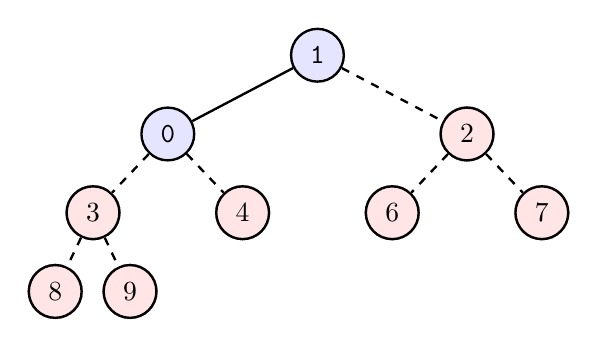
\begin{tikzpicture}

\fill[blue!10] (0.0, 0.0) circle (0.35);
\node [line width=0.03cm,black,minimum size=0.6699999999999999cm,draw,circle] at (0.0,0.0)(1){};\draw (0.0, 0.0) node[color=black] {\texttt{1}};
\fill[blue!10] (-1.9, -1.0) circle (0.35);
\node [line width=0.03cm,black,minimum size=0.6699999999999999cm,draw,circle] at (-1.9,-1.0)(0){};\draw (-1.9, -1.0) node[color=black] {\texttt{0}};
\fill[blue!10] (1.9, -1.0) circle (0.35);
\node [line width=0.03cm,black,minimum size=0.6699999999999999cm,draw,circle] at (1.9,-1.0)(2){};\draw (1.9, -1.0) node[color=black] {\texttt{2}};
\fill[blue!10] (-2.85, -2.0) circle (0.35);
\node [line width=0.03cm,black,minimum size=0.6699999999999999cm,draw,circle] at (-2.85,-2.0)(3){};\draw (-2.85, -2.0) node[color=black] {\texttt{3}};
\fill[blue!10] (-0.95, -2.0) circle (0.35);
\node [line width=0.03cm,black,minimum size=0.6699999999999999cm,draw,circle] at (-0.95,-2.0)(4){};\draw (-0.95, -2.0) node[color=black] {\texttt{4}};
\fill[blue!10] (0.95, -2.0) circle (0.35);
\node [line width=0.03cm,black,minimum size=0.6699999999999999cm,draw,circle] at (0.95,-2.0)(6){};\draw (0.95, -2.0) node[color=black] {\texttt{6}};
\fill[blue!10] (2.85, -2.0) circle (0.35);
\node [line width=0.03cm,black,minimum size=0.6699999999999999cm,draw,circle] at (2.85,-2.0)(7){};\draw (2.85, -2.0) node[color=black] {\texttt{7}};
\fill[blue!10] (-3.33, -3.0) circle (0.35);
\node [line width=0.03cm,black,minimum size=0.6699999999999999cm,draw,circle] at (-3.33,-3.0)(8){};\draw (-3.33, -3.0) node[color=black] {\texttt{8}};
\fill[blue!10] (-2.38, -3.0) circle (0.35);
\node [line width=0.03cm,black,minimum size=0.6699999999999999cm,draw,circle] at (-2.38,-3.0)(9){};\draw (-2.38, -3.0) node[color=black] {\texttt{9}};\draw[line width=0.03cm,black] (1) to  (0);
\draw[line width=0.03cm,black] (1) to  (2);
\draw[line width=0.03cm,black] (0) to  (3);
\draw[line width=0.03cm,black] (0) to  (4);
\draw[line width=0.03cm,black] (2) to  (6);
\draw[line width=0.03cm,black] (2) to  (7);
\draw[line width=0.03cm,black] (3) to  (8);
\draw[line width=0.03cm,black] (3) to  (9);

\fill[red!10] (-2.38, -3.0) circle (0.35);
\draw[line width=0.03cm,black] (-2.38, -3.0) circle (0.33499999999999996);\draw (-2.38, -3.0) node[color=black] {9};
\fill[red!10] (-3.33, -3.0) circle (0.35);
\draw[line width=0.03cm,black] (-3.33, -3.0) circle (0.33499999999999996);\draw (-3.33, -3.0) node[color=black] {8};
\fill[red!10] (2.85, -2.0) circle (0.35);
\draw[line width=0.03cm,black] (2.85, -2.0) circle (0.33499999999999996);\draw (2.85, -2.0) node[color=black] {7};
\fill[red!10] (0.95, -2.0) circle (0.35);
\draw[line width=0.03cm,black] (0.95, -2.0) circle (0.33499999999999996);\draw (0.95, -2.0) node[color=black] {6};
\fill[red!10] (-0.95, -2.0) circle (0.35);
\draw[line width=0.03cm,black] (-0.95, -2.0) circle (0.33499999999999996);\draw (-0.95, -2.0) node[color=black] {4};
\fill[red!10] (-2.85, -2.0) circle (0.35);
\draw[line width=0.03cm,black] (-2.85, -2.0) circle (0.33499999999999996);\draw (-2.85, -2.0) node[color=black] {3};
\fill[red!10] (1.9, -1.0) circle (0.35);
\draw[line width=0.03cm,black] (1.9, -1.0) circle (0.33499999999999996);\draw (1.9, -1.0) node[color=black] {2};\draw[line width=0.1cm,white] (1) to  (2);
\draw[line width=0.03cm,black,,dashed] (1) to  (2);
\draw[line width=0.1cm,white] (3) to  (9);
\draw[line width=0.03cm,black,,dashed] (3) to  (9);
\draw[line width=0.1cm,white] (3) to  (8);
\draw[line width=0.03cm,black,,dashed] (3) to  (8);
\draw[line width=0.1cm,white] (2) to  (7);
\draw[line width=0.03cm,black,,dashed] (2) to  (7);
\draw[line width=0.1cm,white] (2) to  (6);
\draw[line width=0.03cm,black,,dashed] (2) to  (6);
\draw[line width=0.1cm,white] (0) to  (4);
\draw[line width=0.03cm,black,,dashed] (0) to  (4);
\draw[line width=0.1cm,white] (0) to  (3);
\draw[line width=0.03cm,black,,dashed] (0) to  (3);
\end{tikzpicture}

\end{center}


from latextool_basic import *
p = Plot()
xs = [1, 0, 2, 3, 4, 6, 7, 8, 9]
edges = array_to_edges(xs)
pos = drawheap(p, edges, include_array=False)

x,y = pos[9]; p += Graph.node(x=x, y=y, r=BinTree.node_width, background='red!10', label='9')
x,y = pos[8]; p += Graph.node(x=x, y=y, r=BinTree.node_width, background='red!10', label='8')
x,y = pos[7]; p += Graph.node(x=x, y=y, r=BinTree.node_width, background='red!10', label='7')
x,y = pos[6]; p += Graph.node(x=x, y=y, r=BinTree.node_width, background='red!10', label='6')
x,y = pos[4]; p += Graph.node(x=x, y=y, r=BinTree.node_width, background='red!10', label='4')
x,y = pos[3]; p += Graph.node(x=x, y=y, r=BinTree.node_width, background='red!10', label='3')
x,y = pos[2]; p += Graph.node(x=x, y=y, r=BinTree.node_width, background='red!10', label='2')

p += Graph.edge(names=[1,2], linecolor='white', linewidth=0.1); p += Graph.edge(names=[1,2], linestyle='dashed')
p += Graph.edge(names=[3,9], linecolor='white', linewidth=0.1); p += Graph.edge(names=[3,9], linestyle='dashed')
p += Graph.edge(names=[3,8], linecolor='white', linewidth=0.1); p += Graph.edge(names=[3,8], linestyle='dashed')
p += Graph.edge(names=[2,7], linecolor='white', linewidth=0.1); p += Graph.edge(names=[2,7], linestyle='dashed')
p += Graph.edge(names=[2,6], linecolor='white', linewidth=0.1); p += Graph.edge(names=[2,6], linestyle='dashed')
p += Graph.edge(names=[0,4], linecolor='white', linewidth=0.1); p += Graph.edge(names=[0,4], linestyle='dashed')
p += Graph.edge(names=[0,3], linecolor='white', linewidth=0.1); p += Graph.edge(names=[0,3], linestyle='dashed')

print(p)
\begin{center}
\begin{tikzpicture}

\fill[white] (0.0, 0.0) circle (0.3);
\node [line width=0.03cm,black,minimum size=0.57cm,draw,circle] at (0.0,0.0)(10){};\draw (0.0, 0.0) node[color=black] {\texttt{10}};
\fill[white] (-3.0, -1.0) circle (0.35);
\node [line width=0.1cm,red,minimum size=0.6cm,draw,circle] at (-3.0,-1.0)(5){};\draw (-3.0, -1.0) node[color=black] {\texttt{5}};
\fill[white] (3.0, -1.0) circle (0.3);
\node [line width=0.03cm,black,minimum size=0.57cm,draw,circle] at (3.0,-1.0)(18){};\draw (3.0, -1.0) node[color=black] {\texttt{18}};
\fill[white] (-4.5, -2.0) circle (0.3);
\node [line width=0.03cm,black,minimum size=0.57cm,draw,circle] at (-4.5,-2.0)(2){};\draw (-4.5, -2.0) node[color=black] {\texttt{2}};
\fill[white] (-5.25, -3.0) circle (0.3);
\node [line width=0.03cm,black,minimum size=0.57cm,draw,circle] at (-5.25,-3.0)(0){};\draw (-5.25, -3.0) node[color=black] {\texttt{0}};\draw[line width=0.03cm,black,->,>=triangle 60] (10) to  (5);
\draw[line width=0.03cm,black,->,>=triangle 60] (10) to  (18);
\draw[line width=0.1cm,red,->,>=triangle 60] (5) to  (2);
\draw[line width=0.1cm,red,->,>=triangle 60] (2) to  (0);
\end{tikzpicture}

\end{center}


from latextool_basic import *
p = Plot()
a = Array2d(0, 0, width=0.6, height=0.6, 
             xs=[['1','0','2','3','4','6','7','8','9']])
p += a
p0 = a[0][1].bottomright(); p0 = (p0[0], p0[1] - 0.2)
p1 = a[0][1].topright(); p1 = (p1[0], p1[1] + 0.2)
p += Line(points=[p0, p1], linewidth=0.1)
p += Rect(x0=0, y0=-1, x1=2, y1=-1, s=r'\texttt{len = 2}', linewidth=0) 
print(p)


\textsc{Step 8}.
I swap \texttt{1} and \texttt{0}

\begin{center}
\begin{tikzpicture}

\fill[white] (0.0, 0.0) circle (0.3);
\node [line width=0.03cm,black,minimum size=0.57cm,draw,circle] at (0.0,0.0)(10){};\draw (0.0, 0.0) node[color=black] {\texttt{10}};
\fill[white] (-1.5, -1.0) circle (0.35);
\node [line width=0.1cm,red,minimum size=0.6cm,draw,circle] at (-1.5,-1.0)(2){};\draw (-1.5, -1.0) node[color=black] {\texttt{2}};
\fill[white] (1.5, -1.0) circle (0.3);
\node [line width=0.03cm,black,minimum size=0.57cm,draw,circle] at (1.5,-1.0)(18){};\draw (1.5, -1.0) node[color=black] {\texttt{18}};
\fill[white] (-2.25, -2.0) circle (0.3);
\node [line width=0.03cm,black,minimum size=0.57cm,draw,circle] at (-2.25,-2.0)(0){};\draw (-2.25, -2.0) node[color=black] {\texttt{0}};
\fill[white] (-0.75, -2.0) circle (0.3);
\node [line width=0.03cm,black,minimum size=0.57cm,draw,circle] at (-0.75,-2.0)(5){};\draw (-0.75, -2.0) node[color=black] {\texttt{5}};\draw[line width=0.03cm,black,->,>=triangle 60] (10) to  (2);
\draw[line width=0.03cm,black,->,>=triangle 60] (10) to  (18);
\draw[line width=0.03cm,black,->,>=triangle 60] (2) to  (0);
\draw[line width=0.03cm,black,->,>=triangle 60] (2) to  (5);
\end{tikzpicture}

\end{center}


from latextool_basic import *
p = Plot()
xs = [0, 1, 2, 3, 4, 6, 7, 8, 9]
edges = array_to_edges(xs)
pos = drawheap(p, edges, include_array=False)

x,y = pos[9]; p += Graph.node(x=x, y=y, r=BinTree.node_width, background='red!10', label='9')
x,y = pos[8]; p += Graph.node(x=x, y=y, r=BinTree.node_width, background='red!10', label='8')
x,y = pos[7]; p += Graph.node(x=x, y=y, r=BinTree.node_width, background='red!10', label='7')
x,y = pos[6]; p += Graph.node(x=x, y=y, r=BinTree.node_width, background='red!10', label='6')
x,y = pos[4]; p += Graph.node(x=x, y=y, r=BinTree.node_width, background='red!10', label='4')
x,y = pos[3]; p += Graph.node(x=x, y=y, r=BinTree.node_width, background='red!10', label='3')
x,y = pos[2]; p += Graph.node(x=x, y=y, r=BinTree.node_width, background='red!10', label='2')
x,y = pos[1]; p += Graph.node(x=x, y=y, r=BinTree.node_width, background='red!10', label='1')

p += Graph.edge(names=[3,9], linecolor='white', linewidth=0.1); p += Graph.edge(names=[3,9], linestyle='dashed')
p += Graph.edge(names=[3,8], linecolor='white', linewidth=0.1); p += Graph.edge(names=[3,8], linestyle='dashed')
p += Graph.edge(names=[2,7], linecolor='white', linewidth=0.1); p += Graph.edge(names=[2,7], linestyle='dashed')
p += Graph.edge(names=[2,6], linecolor='white', linewidth=0.1); p += Graph.edge(names=[2,6], linestyle='dashed')
p += Graph.edge(names=[1,4], linecolor='white', linewidth=0.1); p += Graph.edge(names=[1,4], linestyle='dashed')
p += Graph.edge(names=[1,3], linecolor='white', linewidth=0.1); p += Graph.edge(names=[1,3], linestyle='dashed')
p += Graph.edge(names=[0,1], linecolor='white', linewidth=0.1); p += Graph.edge(names=[0,1], linestyle='dashed')
p += Graph.edge(names=[0,2], linecolor='white', linewidth=0.1); p += Graph.edge(names=[0,2], linestyle='dashed')

print(p)

Clearly there's no need to heapify-down since the tree now has size 1.
At this point, the array is
\begin{center}
\begin{tikzpicture}

\fill[white] (0.0, 0.0) circle (0.3);
\node [line width=0.03cm,black,minimum size=0.57cm,draw,circle] at (0.0,0.0)(10){};\draw (0.0, 0.0) node[color=black] {\texttt{10}};
\fill[white] (-3.0, -1.0) circle (0.3);
\node [line width=0.03cm,black,minimum size=0.57cm,draw,circle] at (-3.0,-1.0)(2){};\draw (-3.0, -1.0) node[color=black] {\texttt{2}};
\fill[white] (3.0, -1.0) circle (0.3);
\node [line width=0.03cm,black,minimum size=0.57cm,draw,circle] at (3.0,-1.0)(18){};\draw (3.0, -1.0) node[color=black] {\texttt{18}};
\fill[white] (-4.5, -2.0) circle (0.3);
\node [line width=0.03cm,black,minimum size=0.57cm,draw,circle] at (-4.5,-2.0)(0){};\draw (-4.5, -2.0) node[color=black] {\texttt{0}};
\fill[white] (-1.5, -2.0) circle (0.3);
\node [line width=0.03cm,black,minimum size=0.57cm,draw,circle] at (-1.5,-2.0)(5){};\draw (-1.5, -2.0) node[color=black] {\texttt{5}};
\fill[white] (-2.25, -3.0) circle (0.3);
\node [line width=0.03cm,black,minimum size=0.57cm,draw,circle] at (-2.25,-3.0)(3){};\draw (-2.25, -3.0) node[color=black] {\texttt{3}};\draw[line width=0.1cm,red,->,>=triangle 60] (10) to  (2);
\draw[line width=0.03cm,black,->,>=triangle 60] (10) to  (18);
\draw[line width=0.03cm,black,->,>=triangle 60] (2) to  (0);
\draw[line width=0.1cm,red,->,>=triangle 60] (2) to  (5);
\draw[line width=0.1cm,red,->,>=triangle 60] (5) to  (3);
\end{tikzpicture}

\end{center}


from latextool_basic import *
p = Plot()
a = Array2d(0, 0, width=0.6, height=0.6, 
             xs=[['0','1','2','3','4','6','7','8','9']])
p += a
p0 = a[0][0].bottomright(); p0 = (p0[0], p0[1] - 0.2)
p1 = a[0][0].topright(); p1 = (p1[0], p1[1] + 0.2)
p += Line(points=[p0, p1], linewidth=0.1)
p += Rect(x0=0, y0=-1, x1=2, y1=-1, s=r'\texttt{len = 1}', linewidth=0) 
print(p)
It's sorted!

Here's the algorithm:
\begin{console}
ALGORITHM: heapsort
INPUT:     x - array
           n - length of x

Perform build_maxheap on x[0..n - 1]
for i = n - 1, n - 2, ..., 1: 
    swap x[0] and x[i]
    perform heapify_down on x[0..i - 1] at index 0
\end{console}

\newpage
\begin{ex}
Perform heapsort on given arrays below (in ascending order).
Execute build-maxheap and then continually perform
extract-max and heapify.
Draw the tree after every extract-max and heapify and draw the
corresponding array.
\begin{tightlist}
  \li \verb![5, 7, 4, 0, 8]!
  \li \verb![3, 9, 0, 7, 2, 5, 4, 1, 0]!
  \li \verb![1, 3, 5, 7, 6, 4, 2, 0, 8, 9]!
  \li \verb![0, 1, 2, 3, 4, 5, 6, 7, 8, 9]!
  \li \verb![9, 8, 7, 6, 5, 4, 3, 2, 1, 0]!
\end{tightlist}
\end{ex}

\newpage
\begin{ex}
  Now do the same as above
  except that you perform heapsort in \textit{descending} order.
\begin{tightlist}
  \li \verb![5, 7, 4, 0, 8]!
  \li \verb![3, 9, 0, 7, 2, 5, 4, 1, 0]!
  \li \verb![1, 3, 5, 7, 6, 4, 2, 0, 8, 9]!
  \li \verb![0, 1, 2, 3, 4, 5, 6, 7, 8, 9]!
  \li \verb![9, 8, 7, 6, 5, 4, 3, 2, 1, 0]!
\end{tightlist}
\end{ex}


\newpage
\begin{ex}
An array $x$ of size $n$ represents a maxheap.
What is the fastest way to find the minimum value in $x$?
\qed
\end{ex}
% The minimum must be a leave. Look at $n/2, ..., n - 1$.
% n-1 - n/2 + 1 = n - n / 2 accesses.


\newpage
\begin{ex}
Figure out a good algorithmn to merge two maxheaps.
\qed
\end{ex}



%\newpage%-*-latex-*-
\sectionthree{Merge}
\begin{python0}
from solutions import *; clear()
\end{python0}

Suppose you're two max heaps.
Is there an efficient way to put them together to get a max heap?
This is called a heap \defone{merge} or a heap \defone{union}.

For instance suppose, suppose a machine has
two exact same server process running the same software,
answering to HTTP requests.
Each server software maintains it's own queue of server requests.
However something bad happened: one of the server process is stuck
(hackers?)
A main master process that watches the two server processes
sees that one of server processes is stuck.
So it transfers the queue of requests to the one that is still alive
and kills the server that is stuck.
Somehow the two queues of requests has to be merged.

By the way.
I hope you realize that if you have a max heap and you remove the
root, then the two subtrees are themselves max heaps.
For instance if you remove the root from this max heap:


\begin{center}

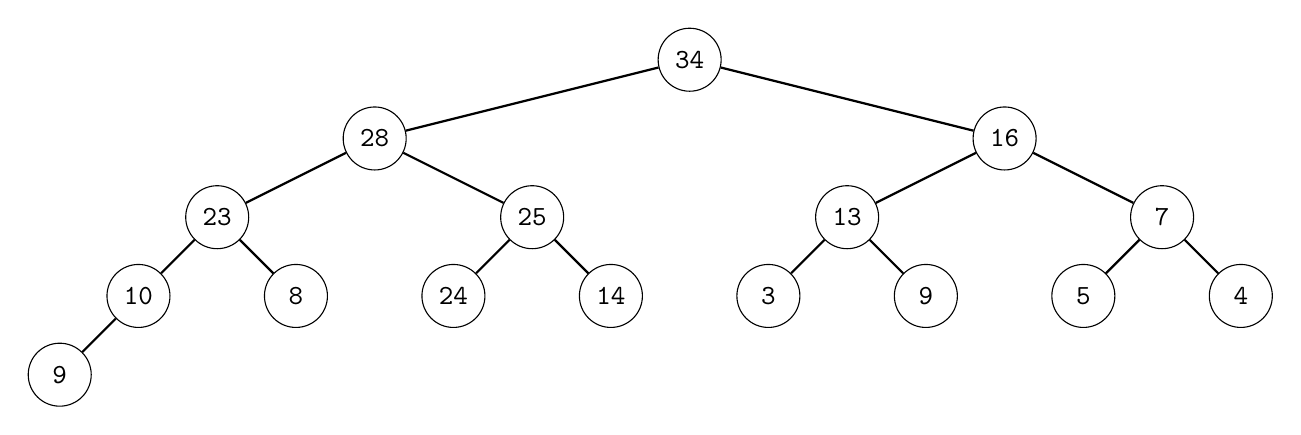
\begin{tikzpicture}
\node at (8,-1) [circle,draw,minimum size=8mm] (A) {\texttt{34}};
\node at (4,-2) [circle,draw,minimum size=8mm] (B) {\texttt{28}};
\node at (12,-2) [circle,draw,minimum size=8mm] (C) {\texttt{16}};
\node at (2,-3) [circle,draw,minimum size=8mm] (D) {\texttt{23}};
\node at (6,-3) [circle,draw,minimum size=8mm] (E) {\texttt{25}};
\node at (10,-3) [circle,draw,minimum size=8mm] (F) {\texttt{13}};
\node at (14,-3) [circle,draw,minimum size=8mm] (G) {\texttt{7}};
\node at (1,-4) [circle,draw,minimum size=8mm] (H) {\texttt{10}};
\node at (3,-4) [circle,draw,minimum size=8mm] (I) {\texttt{8}};
\node at (5,-4) [circle,draw,minimum size=8mm] (J) {\texttt{24}};
\node at (7,-4) [circle,draw,minimum size=8mm] (K) {\texttt{14}};
\node at (9,-4) [circle,draw,minimum size=8mm] (L) {\texttt{3}};
\node at (11,-4) [circle,draw,minimum size=8mm] (M) {\texttt{9}};
\node at (13,-4) [circle,draw,minimum size=8mm] (N) {\texttt{5}};
\node at (15,-4) [circle,draw,minimum size=8mm] (O) {\texttt{4}};
\node at (0,-5) [circle,draw,minimum size=8mm] (P) {\texttt{9}};
\draw [-,thick] (A) -- (B);
\draw [-,thick] (A) -- (C);
\draw [-,thick] (B) -- (D);
\draw [-,thick] (B) -- (E);
\draw [-,thick] (C) -- (G);
\draw [-,thick] (C) -- (F);
\draw [-,thick] (D) -- (H);
\draw [-,thick] (D) -- (I);
\draw [-,thick] (E) -- (J);
\draw [-,thick] (E) -- (K);
\draw [-,thick] (F) -- (L);
\draw [-,thick] (F) -- (M);
\draw [-,thick] (G) -- (N);
\draw [-,thick] (G) -- (O);
\draw [-,thick] (H) -- (P);

;
\end{tikzpicture}
    
\end{center}



you get the left subtree which is a max heap:

\begin{center}
\begin{tikzpicture}

\fill[white] (0.0, 0.0) circle (0.3);
\node [line width=0.03cm,black,minimum size=0.57cm,draw,circle] at (0.0,0.0)(5){};\draw (0.0, 0.0) node[color=black] {\texttt{5}};
\fill[white] (-1.5, -1.0) circle (0.3);
\node [line width=0.03cm,black,minimum size=0.57cm,draw,circle] at (-1.5,-1.0)(2){};\draw (-1.5, -1.0) node[color=black] {\texttt{2}};
\fill[white] (1.5, -1.0) circle (0.3);
\node [line width=0.03cm,black,minimum size=0.57cm,draw,circle] at (1.5,-1.0)(10){};\draw (1.5, -1.0) node[color=black] {\texttt{10}};
\fill[white] (-2.25, -2.0) circle (0.3);
\node [line width=0.03cm,black,minimum size=0.57cm,draw,circle] at (-2.25,-2.0)(0){};\draw (-2.25, -2.0) node[color=black] {\texttt{0}};
\fill[white] (-0.75, -2.0) circle (0.3);
\node [line width=0.03cm,black,minimum size=0.57cm,draw,circle] at (-0.75,-2.0)(3){};\draw (-0.75, -2.0) node[color=black] {\texttt{3}};
\fill[white] (2.25, -2.0) circle (0.3);
\node [line width=0.03cm,black,minimum size=0.57cm,draw,circle] at (2.25,-2.0)(18){};\draw (2.25, -2.0) node[color=black] {\texttt{18}};\draw[line width=0.03cm,black,->,>=triangle 60] (5) to  (2);
\draw[line width=0.03cm,black,->,>=triangle 60] (5) to  (10);
\draw[line width=0.03cm,black,->,>=triangle 60] (10) to  (18);
\draw[line width=0.03cm,black,->,>=triangle 60] (2) to  (0);
\draw[line width=0.03cm,black,->,>=triangle 60] (2) to  (3);
\end{tikzpicture}

\end{center}



and the right subtree which is also a max heap:


\begin{center}

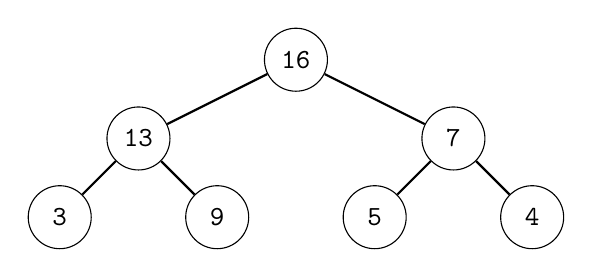
\begin{tikzpicture}
\node at (3,-1) [circle,draw,minimum size=8mm] (C) {\texttt{16}};
\node at (1,-2) [circle,draw,minimum size=8mm] (F) {\texttt{13}};
\node at (5,-2) [circle,draw,minimum size=8mm] (G) {\texttt{7}};
\node at (0,-3) [circle,draw,minimum size=8mm] (L) {\texttt{3}};
\node at (2,-3) [circle,draw,minimum size=8mm] (M) {\texttt{9}};
\node at (4,-3) [circle,draw,minimum size=8mm] (N) {\texttt{5}};
\node at (6,-3) [circle,draw,minimum size=8mm] (O) {\texttt{4}};
\draw [-,thick] (C) -- (G);
\draw [-,thick] (C) -- (F);
\draw [-,thick] (F) -- (L);
\draw [-,thick] (F) -- (M);
\draw [-,thick] (G) -- (N);
\draw [-,thick] (G) -- (O);

;
\end{tikzpicture}
    
\end{center}



OK.
Back to the algorithm of merging two (max) heaps $H_0$ and $H_1$.
Suppose the total number of nodes in $H_1$ is $m$
and the total number of nodes in $H_2$ is $n$.
Without using the existing heap structure in $H_1$ and $H_2$
and just build a heap from scratch requires $O(n)$ using the build-heap
operation.
Also, note that if we can merge two heaps quickly,
then another way to build a heap is to do it recursively:
recursive divide a collection of values into two piles,
make them into heaps, then merge the heaps.
So what's there not to like?

However, for our max heap, the only way seems to be to copy the
values from one heap to another and perform build-heap
which will run in $O(m + n)$
where $m$ is the size of the first heap and $n$ is the size of the second.



\begin{ex} 
  \label{ex:some-decision1}
  \tinysidebar{\debug{exercises/{empty0/question.tex}}}
  \solutionlink{sol:some-decision1}
  \qed
\end{ex} 
\begin{python0}
from solutions import *
add(label="ex:some-decision1",
    srcfilename='exercises/some-decision1/answer.tex') 
\end{python0}


\begin{comment}
\begin{center}
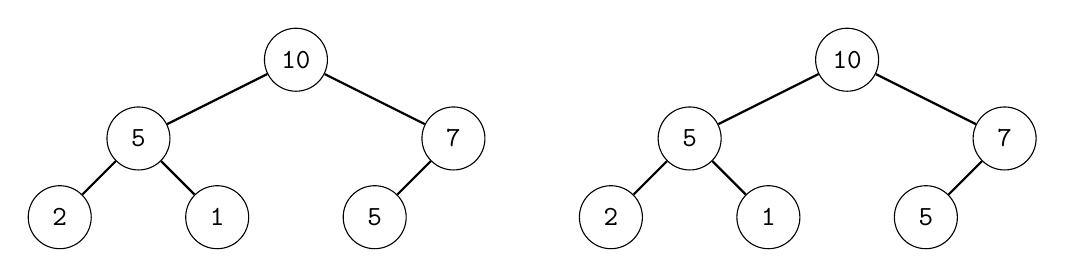
\begin{tikzpicture}


\node at (3,-1) [circle,draw,minimum size=8mm] (A) {\texttt{10}};
\node at (1,-2) [circle,draw,minimum size=8mm] (B) {\texttt{5}};
\node at (5,-2) [circle,draw,minimum size=8mm] (C) {\texttt{7}};
\node at (0,-3) [circle,draw,minimum size=8mm] (D) {\texttt{2}};
\node at (2,-3) [circle,draw,minimum size=8mm] (E) {\texttt{1}};
\node at (4,-3) [circle,draw,minimum size=8mm] (G) {\texttt{5}};
\draw [-,thick] (A) -- (B);
\draw [-,thick] (A) -- (C);
\draw [-,thick] (B) -- (D);
\draw [-,thick] (B) -- (E);
\draw [-,thick] (C) -- (G);

;

    

\node at (10,-1) [circle,draw,minimum size=8mm] (A) {\texttt{10}};
\node at (8,-2) [circle,draw,minimum size=8mm] (B) {\texttt{5}};
\node at (12,-2) [circle,draw,minimum size=8mm] (C) {\texttt{7}};
\node at (7,-3) [circle,draw,minimum size=8mm] (D) {\texttt{2}};
\node at (9,-3) [circle,draw,minimum size=8mm] (E) {\texttt{1}};
\node at (11,-3) [circle,draw,minimum size=8mm] (G) {\texttt{5}};
\draw [-,thick] (A) -- (B);
\draw [-,thick] (A) -- (C);
\draw [-,thick] (B) -- (D);
\draw [-,thick] (B) -- (E);
\draw [-,thick] (C) -- (G);

;
\end{tikzpicture}

\end{center}


[Instead of max heap, what is the levels are
coordinates?
I.e., the max is root,
the 2nd and 3rd at level 1,
the 4th,5th,6th,7th at level 2, etc.
If so, then during merge, to new heap's root is one of the two roots.
Say the first heap has a large root.
Then heap1's level 0 is done.
For level 1 of teh new heap, we look at level 1 of heap1
and level0 of heap2.
Etc.

\input{stdout92.tex}

In the above, 16 should probably be moved the the subtree at 28.
Who can replaced 16?
The max of 16's children is 13.
Or just looking at the subtree at 16, maybe it's better to switch 7 and 9:

\begin{center}
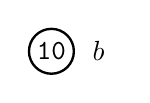
\begin{tikzpicture}

\fill[white] (0.0, 0.0) circle (0.3);
\node [line width=0.03cm,black,minimum size=0.57cm,draw,circle] at (0.0,0.0)(10){};\draw (0.0, 0.0) node[color=black] {\texttt{10}};
\fill[white] (0.6, 0.0) circle (0.3);
\node [draw=none,line width=0cm,black,minimum size=0.6cm,circle] at (0.6,0.0){};\draw (0.6, 0.0) node[color=black] {$b$};
\end{tikzpicture}

\end{center}



or

\begin{center}
\begin{tikzpicture}

\fill[white] (0.0, 0.0) circle (0.3);
\node [line width=0.03cm,black,minimum size=0.57cm,draw,circle] at (0.0,0.0)(10){};\draw (0.0, 0.0) node[color=black] {\texttt{10}};
\draw (1.3, 0.0)
  node[draw=none, line width=0cm, , color=black,
       rounded corners=0cm, inner sep=0cm] {

\begin{minipage}[t][0.1cm]{0.1cm}
\mbox{}

\end{minipage}

};\draw (1.3, 0.0) node[color=black] {$b \rightarrow b - 1$};
\fill[white] (-0.75, -1.0) circle (0.3);
\node [line width=0.03cm,black,minimum size=0.57cm,draw,circle] at (-0.75,-1.0)(5){};\draw (-0.75, -1.0) node[color=black] {\texttt{5}};
\fill[white] (-0.14999999999999997, -1.0) circle (0.3);
\node [draw=none,line width=0cm,black,minimum size=0.6cm,circle] at (-0.14999999999999997,-1.0){};\draw (-0.14999999999999997, -1.0) node[color=black] {0};\draw[line width=0.03cm,black,->,>=triangle 60] (10) to  (5);
\end{tikzpicture}

\end{center}



]
\end{comment}

\newpage%-*-latex-*-
\section{Compare heap against queue and BST/AVL}

As mentioned earlier, the point of the heap is to
organized data so that you want remove an item
with the highest priority (use maxheap or minheap depending
on whether \lq\lq higher prioriy" mean \lq\lq larger priority number"
or \lq\lq smaller priority number".

Here is the runtimes of the heap (min or max):
\begin{enumerate}[nosep]
\item Insert: $O(\lg n)$
\item Delete: $O(\lg n)$ (i.e., delete the root)
\end{enumerate}
Of course if you just want to peek at the highest priority value without deleting it,
it's $O(1)$.

If you use a queue (using double linked list) to implement a 
priority queue,
\begin{enumerate}[nosep]
\item Insert: $O(n)$
\item Delete: $O(1)$ (i.e., delete the root)
\end{enumerate}
You might think this is OK since the delete is fast.
But hang on cowboy ... if you perform $n$ inserts and deletes 
say alternativing them, the average is going to be $O(n)$ for each.
The average for the heap is going to be $O(\lg n)$.
So using a queue is a bad idea.

What about a BST? Say we use the AVL tree.
\begin{enumerate}[nosep]
\item Insert: $O(\lg n)$
\item Delete: $O(\lg n)$ (i.e., delete the minimum)
\end{enumerate}
If you want to peek at the minimum without removing it,
the runtime is $O(\lg n)$.
Excluding the peek, the insert and delete are the 
same as the heap.
But wait ...

When you insert a value into an AVL, what is the runtime?
The value is inserted as a leaf. The runtime is not just worst
runtime of $O(\lg n)$. It is in fact exactly $\Theta(\lg n)$.

But what about a heap? Say a minheap?
While in the case of the AVL tree, you have to walk from the root
to a leaf, in the case of the insert into a minheap,
you insert at the leaf and you heapify-up -- but the
heapify-up might stop \textit{anywhere} along the way to the root.

Assuming the tree is full.
How many leaves are there? If the height is $h$,
then there are $2^{h + 1}$ leaves.
And how many nonleaves are there?
Well it's $1 + 2 + \cdots + 2^{h} = 2^{h+1} - 1$.
So there's a 50\% chance that the inserted value is a leaf!
Which in the case of a heap, it means that there's not
a whole lot of heapify up at all!!!
In fact you can show (but you would need probability theory)
that the \textit{average} runtime of heap insert is $O(1)$.

Wonderful! 

\newpage%-*-latex-*-
%
% https://www.fluentcpp.com/2019/10/29/stdless-and-its-modern-evolution/
%

\section{API}

Here I'm assuming the implementation is an array-based implementation
(for us, this means C array or C++ \verb!std::vector! objects).
Here are some very common operations:

\begin{longtable}{l|l}
\hline
\texttt{is\_heap}                   & true if it's a heap \\
\texttt{heap\_insert}               & insert a value into a heap \\
\texttt{heap\_delete/extract-root}  & delete max (min) in a maxheap (minheap) \\
\texttt{build\_heap}           & create a heap from the array) \\
\texttt{root}                  & return reference to the root of the heap \\
\texttt{heapsort}              & heapsort on array \\
\hline
\end{longtable}
(Another important operation is to merge two heaps into one.)
Since I am using an array or \verb!std::vector!, the function \verb!root!
is redundant.

It's kind of annoying to have to use max/min in the names above.
The simplest thing to do is to define a comparison function that the
heap functions/class uses.
The boolean function basically compares two nodes and tells you
which node should be \lq\lq higher" in the heap tree.

\newpage%-*-latex-*-
\section{Implementing min- and maxheaps at the same time}

(You want to review \verb!std::vector!, iterators,
function pointers and functors.)

With function pointers or functors, you can write a heapify-up (and heapify-down)
function that works for both maxheap and minheap
simply by passing in a comparison function or functor.

\begin{Verbatim}[frame=single, fontsize=\small]
#include <iostream>

bool less(int x, int y)
{
    return (x < y);
}
  
bool greater(int x, int y) 
{
    return (x > y);
}

void heapify_up(int x[], int n, int i, bool (*cmp)(int, int))
{
    int v = x[i];
    while (1)
    {
        int p = (i - 1) / 2;
        if (cmp(x[i], x[p]))
        {
            x[p] = x[i];
            i = p;
        }
        else
        {
            x[i] = v;
            break;
        }
    }
}

int main()
{
    f(less);
    return 0;
}
\end{Verbatim}
The next thing is to make heapify up into a template:
\begin{Verbatim}[frame=single, fontsize=\small]
template < typename T >
bool less(const T & x, const T & y)
{
    return (x < y);
}
  
template < typename T >
bool greater(const T & x, const T & y)
{
    return (x > y);
}

template < typename T >
void heapify_up(T x[], int n, int i, bool (*cmp)(T, T))
{
    T v = x[i];
    ...
}
\end{Verbatim}

Another way to achieve this is through functors.
\begin{Verbatim}[frame=single, fontsize=\small]
template < typename T >
struct less
{
    bool operator()(const T & x, const T & y)
    {
        return (x < y);
    }
};

template < typename T >
struct greater
{
    bool operator()(const T & x, const T & y)
    {
        return (x > y);
    }
};

template < typename T, typename Comparator >
void heapify_up(T x[], int n, int i)
{
    T v = x[i];
    ...
}
\end{Verbatim}






\newpage%-*-latex-*-
\sectionthree{C++ STL heap functions}
\begin{python0}
from solutions import *; clear()
\end{python0}

C++ provides heap functions
which operate on sequential container such as \verb!std::vector!
or arrays.
By default the functions assume the heap is a maxheap.

To use it do this at the top of your cpp file:
\begin{Verbatim}[frame=single, fontsize=\small]
#include <algorithm>
\end{Verbatim}

Let \verb!v! be a \verb!std::vector< T >! object (for some type \verb!T!).
\begin{enumerate}[nosep]
  \li \verb!std::make_heap(v.begin(), v.end())!: make \verb!v! into a maxheap
  \li \verb!std::is_heap(v.begin(), v.end())!: returns \verb!true! if \verb!v! is maxheap
  \li \verb!std::is_heap_until(v.begin(), v.end())!:
  return iterator pointing to first value that violates maxheap property.
  If \verb!v! is maxheap, !v.end()! is returned.
  \li \verb!std::push_heap(v.begin(), v.end())!: Performs heapify-up on
  the last entry of \verb!v!.
  So to perform a maxheap insert with \verb!x!, you would first
  do \verb!v.push_back(x)! and then execute
  \verb!std::push_heap(v.begin(), v.end())!.
  \li \verb!std::pop_heap(v.begin(), v.end())!: Performs extract-root,
  but instead of removing the root,
  the root is placed at the last value entry of \verb!v!.
  So to perform a maxheap delete, you would first
  do \verb!std::pop_heap(v.begin(), v.end())!
  and then \verb!v.pop_back(x)!.
  \li \verb!std::sort_heap(v.begin(), v.end()!: heapsort assuming the
  vector is already a maxheap.
\end{enumerate}
All the functions above can also accept an extra comparator functor.
\begin{center}
\begin{tikzpicture}

\fill[white] (0.0, 0.0) circle (0.3);
\node [line width=0.03cm,black,minimum size=0.57cm,draw,circle] at (0.0,0.0)(10){};\draw (0.0, 0.0) node[color=black] {\texttt{10}};
\fill[white] (1.4, 0.0) circle (0.3);
\node [draw=none,line width=0cm,black,minimum size=0.6cm,circle] at (1.4,0.0){};\draw (1.4, 0.0) node[color=black] {$b \rightarrow b + 1$};
\fill[white] (0.75, -1.0) circle (0.3);
\node [line width=0.03cm,black,minimum size=0.57cm,draw,circle] at (0.75,-1.0)(5){};\draw (0.75, -1.0) node[color=black] {\texttt{5}};
\fill[white] (1.35, -1.0) circle (0.3);
\node [draw=none,line width=0cm,black,minimum size=0.6cm,circle] at (1.35,-1.0){};\draw (1.35, -1.0) node[color=black] {0};\draw[line width=0.03cm,black,->,>=triangle 60] (10) to  (5);
\end{tikzpicture}

\end{center}


Of course you can also use an array:
\begin{center}
\begin{tikzpicture}

\fill[white] (0.0, 0.0) circle (0.3);
\node [line width=0.03cm,black,minimum size=0.57cm,draw,circle] at (0.0,0.0)(25){};\draw (0.0, 0.0) node[color=black] {\texttt{25}};
\fill[white] (0.6, 0.0) circle (0.3);
\node [draw=none,line width=0cm,black,minimum size=0.6cm,circle] at (0.6,0.0){};\draw (0.6, 0.0) node[color=black] {$b'$};
\fill[white] (-1.5, -1.0) circle (0.3);
\node [line width=0.03cm,black,minimum size=0.57cm,draw,circle] at (-1.5,-1.0)(10){};\draw (-1.5, -1.0) node[color=black] {\texttt{10}};
\fill[white] (-0.9, -1.0) circle (0.3);
\node [draw=none,line width=0cm,black,minimum size=0.6cm,circle] at (-0.9,-1.0){};\draw (-0.9, -1.0) node[color=black] {$b$};\draw[line width=0.03cm,black,->,>=triangle 60] (25) to  (10);
\end{tikzpicture}

\end{center}




\begin{ex} 
  \label{ex:some-decision1}
  \tinysidebar{\debug{exercises/{empty0/question.tex}}}
  \solutionlink{sol:some-decision1}
  \qed
\end{ex} 
\begin{python0}
from solutions import *
add(label="ex:some-decision1",
    srcfilename='exercises/some-decision1/answer.tex') 
\end{python0}


%\newpage%-*-latex-*-
\sectionthree{C++ STL \texttt{std::priority\_queue}}
\begin{python0}
from solutions import *; clear()
\end{python0}

C++ provides an STL container \defone{\texttt{std::priority\_queue}}
for ...
priority queues (duh).

Let \verb!priqueue! be a \verb!priority_queue< T >! object
for some type \verb!T!.
Here are some of the methods:
\begin{enumerate}[nosep]
  \li \texttt{priqueue.size()}: number of values in the \verb!priqueue! 
  \li \texttt{priqueue.empty()}: true iff \verb!priqueue! is empty
  \li \texttt{priqueue.top()}: the root of \verb!priqueue!
  \li \texttt{priqueue.pop()}: extract root from \verb!priqueue!
\end{enumerate}

\input{stdout97.tex}

%\newpage%-*-latex-*-
\sectionthree{Implementation}
\begin{python0}
from solutions import *; clear()
\end{python0}

Frequently heaps are implemented using arrays,
i.e., they are array trees.


\begin{ex} 
  \label{ex:some-decision1}
  \tinysidebar{\debug{exercises/{empty0/question.tex}}}
  \solutionlink{sol:some-decision1}
  \qed
\end{ex} 
\begin{python0}
from solutions import *
add(label="ex:some-decision1",
    srcfilename='exercises/some-decision1/answer.tex') 
\end{python0}



\begin{ex} 
  \label{ex:some-decision1}
  \tinysidebar{\debug{exercises/{empty0/question.tex}}}
  \solutionlink{sol:some-decision1}
  \qed
\end{ex} 
\begin{python0}
from solutions import *
add(label="ex:some-decision1",
    srcfilename='exercises/some-decision1/answer.tex') 
\end{python0}


There are 2 ways of doing the above.

Method 1:
For object $x$, instead of using $x.priority$,
use $(priority, time)$ where the minheap maintains
a time that is incremented every time
an insert occurs. The ordering of $(priority, time)$
is dictionary.
For the case of maxheap, decrement the time counter.

Disadvantage: If the heap runs for a very long time,
the time might overflow.

Method 2:
The heap is made up of linked list of values.
Each linked list contains values of the same priority.
When a value $x$ is inserted, if $x.priority$ occurs in
the minheap, insert $x$ into the correct linked list.
If x's priority is new, create a new linked list and
insert into heap.
Note that we need to know if a linked list of the
correct priority exists in the heap.
We can have a hash table of (priority, heap index).
During heap operations (heapify-up and -down), the
hash table must be updated during the swaps.
If the root linked list is empty, it is removed from the heap.
If the heap allows priority modification, then
a non-root linked list can become empty -- this should not be
delete.
Therefore during the extract-root operation,
need to loop over the extract-root operation until
the new root is a non-empty linked list.


\begin{ex} 
  \label{ex:some-decision1}
  \tinysidebar{\debug{exercises/{empty0/question.tex}}}
  \solutionlink{sol:some-decision1}
  \qed
\end{ex} 
\begin{python0}
from solutions import *
add(label="ex:some-decision1",
    srcfilename='exercises/some-decision1/answer.tex') 
\end{python0}


Clearly the following must work: copy constructor, destructor,
\verb!operator=!, \verb!operator==!.
The class should look like this:
\begin{console}
template < typename T >
class MaxHeap
{
public:
private:
    std::vector < T > x;
};
\end{console}


\begin{ex} 
  \label{ex:some-decision1}
  \tinysidebar{\debug{exercises/{empty0/question.tex}}}
  \solutionlink{sol:some-decision1}
  \qed
\end{ex} 
\begin{python0}
from solutions import *
add(label="ex:some-decision1",
    srcfilename='exercises/some-decision1/answer.tex') 
\end{python0}


\section{Non-array implementation}

For a non-array implementation of heaps,
consider this:


\begin{center}

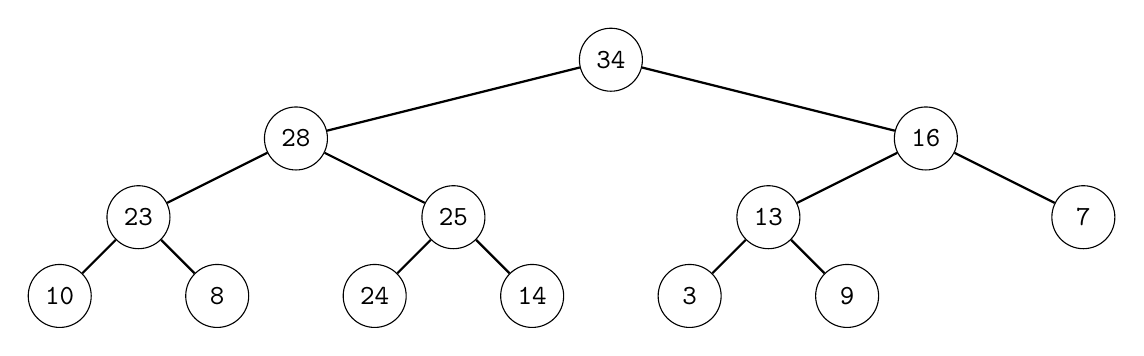
\begin{tikzpicture}
\node at (7,-1) [circle,draw,minimum size=8mm] (A) {\texttt{34}};
\node at (3,-2) [circle,draw,minimum size=8mm] (B) {\texttt{28}};
\node at (11,-2) [circle,draw,minimum size=8mm] (C) {\texttt{16}};
\node at (1,-3) [circle,draw,minimum size=8mm] (D) {\texttt{23}};
\node at (5,-3) [circle,draw,minimum size=8mm] (E) {\texttt{25}};
\node at (9,-3) [circle,draw,minimum size=8mm] (F) {\texttt{13}};
\node at (13,-3) [circle,draw,minimum size=8mm] (G) {\texttt{7}};
\node at (0,-4) [circle,draw,minimum size=8mm] (H) {\texttt{10}};
\node at (2,-4) [circle,draw,minimum size=8mm] (I) {\texttt{8}};
\node at (4,-4) [circle,draw,minimum size=8mm] (J) {\texttt{24}};
\node at (6,-4) [circle,draw,minimum size=8mm] (K) {\texttt{14}};
\node at (8,-4) [circle,draw,minimum size=8mm] (L) {\texttt{3}};
\node at (10,-4) [circle,draw,minimum size=8mm] (M) {\texttt{9}};
\draw [-,thick] (A) -- (B);
\draw [-,thick] (A) -- (C);
\draw [-,thick] (B) -- (D);
\draw [-,thick] (B) -- (E);
\draw [-,thick] (C) -- (G);
\draw [-,thick] (C) -- (F);
\draw [-,thick] (D) -- (H);
\draw [-,thick] (D) -- (I);
\draw [-,thick] (E) -- (J);
\draw [-,thick] (E) -- (K);
\draw [-,thick] (F) -- (L);
\draw [-,thick] (F) -- (M);

;
\end{tikzpicture}
    
\end{center}



Of course I need a pointer to the root.
That's pretty obvious.
Another thing to note is that because of the way I add nodes,
i.e., always at the lowest level and left-to-right, I should have a pointer
to the parent where I have a new node.


\begin{ex} 
  \label{ex:some-decision1}
  \tinysidebar{\debug{exercises/{empty0/question.tex}}}
  \solutionlink{sol:some-decision1}
  \qed
\end{ex} 
\begin{python0}
from solutions import *
add(label="ex:some-decision1",
    srcfilename='exercises/some-decision1/answer.tex') 
\end{python0}


However that takes $(\log n)$ time.
So we might as well have a pointer that records where the
insert should go.
But that's not enough.
Once a level is full, we need to go to the next level.
Therefore we need two (and not one) extra pointer.
Like this:

\input{stdout104.tex}

Note that each node has not just left child and right child pointer.
When we do delete, we might need to go to the previous level.
That means that each node must have a parent pointer too.
Of course the parent pointer is also needed when I do heapify-up, right?

If I insert \texttt{4} to the above, then I get this:

\begin{center}
\begin{tikzpicture}


\node at (7,-1) [circle,draw,minimum size=8mm] (A) {\texttt{34}};
\node at (3,-2) [circle,draw,minimum size=8mm] (B) {\texttt{28}};
\node at (11,-2) [circle,draw,minimum size=8mm] (C) {\texttt{16}};
\node at (1,-3) [circle,draw,minimum size=8mm] (D) {\texttt{23}};
\node at (5,-3) [circle,draw,minimum size=8mm] (E) {\texttt{25}};
\node at (9,-3) [circle,draw,minimum size=8mm] (F) {\texttt{13}};
\node at (13,-3) [circle,draw,minimum size=8mm] (G) {\texttt{7}};
\node at (0,-4) [circle,draw,minimum size=8mm] (H) {\texttt{10}};
\node at (2,-4) [circle,draw,minimum size=8mm] (I) {\texttt{8}};
\node at (4,-4) [circle,draw,minimum size=8mm] (J) {\texttt{24}};
\node at (6,-4) [circle,draw,minimum size=8mm] (K) {\texttt{14}};
\node at (8,-4) [circle,draw,minimum size=8mm] (L) {\texttt{3}};
\node at (10,-4) [circle,draw,minimum size=8mm] (M) {\texttt{9}};
\node at (12,-4) [circle,draw,minimum size=8mm] (N) {\texttt{5}};
\node at (14,-4) [circle,draw,minimum size=8mm] (O) {\texttt{4}};
\draw [-,thick] (A) -- (B);
\draw [-,thick] (A) -- (C);
\draw [-,thick] (B) -- (D);
\draw [-,thick] (B) -- (E);
\draw [-,thick] (C) -- (G);
\draw [-,thick] (C) -- (F);
\draw [-,thick] (D) -- (H);
\draw [-,thick] (D) -- (I);
\draw [-,thick] (E) -- (J);
\draw [-,thick] (E) -- (K);
\draw [-,thick] (F) -- (L);
\draw [-,thick] (F) -- (M);
\draw [-,thick] (G) -- (N);
\draw [-,thick] (G) -- (O);

;

    \node (proot) at (7,0.5) {\texttt{proot}} ;\path [-triangle 60] (proot) edge[] (A);\node (p0) at (0,-5.5) {\texttt{p0}} ;\path [-triangle 60] (p0) edge[] (H);\node (p1) at (14,-5.5) {\texttt{p1}} ;\path [-triangle 60] (p1) edge[] (O);\node (p) at (0,-2.5) {\texttt{p}} ;\path [-triangle 60] (p) edge[] (H);
\end{tikzpicture}

\end{center}



If I add \texttt{8}, I get this:

\input{stdout106.tex}

Once I add a \texttt{9}, I get this:

\input{stdout98.tex}

Get it?

  
Clearly the above idea works for complete trees where
nodes are added left-to-right at the last level.

Note that \verb!p! points to the parent where new nodes should be
attached but does not have information on whether it should be
as a left or as a right child.
You can also include an integer variable \texttt{num\_children}
to tell you how many children
there are.
If the number of children is 0, then the new node should be
attached as a left child.
If the number of children is 1, then the new node should be attached
as a right child.


\begin{ex} 
  \label{ex:some-decision1}
  \tinysidebar{\debug{exercises/{empty0/question.tex}}}
  \solutionlink{sol:some-decision1}
  \qed
\end{ex} 
\begin{python0}
from solutions import *
add(label="ex:some-decision1",
    srcfilename='exercises/some-decision1/answer.tex') 
\end{python0}



\begin{ex} 
  \label{ex:some-decision1}
  \tinysidebar{\debug{exercises/{empty0/question.tex}}}
  \solutionlink{sol:some-decision1}
  \qed
\end{ex} 
\begin{python0}
from solutions import *
add(label="ex:some-decision1",
    srcfilename='exercises/some-decision1/answer.tex') 
\end{python0}


%\newpage%-*-latex-*-
\sectionthree{Fake root heap}
\begin{python0}
from solutions import *; clear()
\end{python0}

Suppose you have two max heaps.
One quick way to merge them is to simply create a new root
and join the new root to the two roots as parent.
The value of the new root can be any arbitrary value that
is larger than the values of the two roots.
To remind myself that the new root is not really a value in the
heap, I can use a flag in each node.
Another thing that I can do it to use a value that is sentinel.
In the case of max heap, say I call this value $\infty$.

For instance say you have these two max heaps:
\begin{center}
\begin{tikzpicture}

\fill[white] (0.0, 0.0) circle (0.3);
\node [line width=0.03cm,black,minimum size=0.57cm,draw,circle] at (0.0,0.0)(10){};\draw (0.0, 0.0) node[color=black] {\texttt{10}};
\fill[white] (-3.0, -1.0) circle (0.3);
\node [line width=0.03cm,black,minimum size=0.57cm,draw,circle] at (-3.0,-1.0)(5){};\draw (-3.0, -1.0) node[color=black] {\texttt{5}};
\fill[white] (3.0, -1.0) circle (0.3);
\node [line width=0.03cm,black,minimum size=0.57cm,draw,circle] at (3.0,-1.0)(15){};\draw (3.0, -1.0) node[color=black] {\texttt{15}};
\fill[white] (-4.5, -2.0) circle (0.3);
\node [line width=0.03cm,black,minimum size=0.57cm,draw,circle] at (-4.5,-2.0)(0){};\draw (-4.5, -2.0) node[color=black] {\texttt{0}};
\fill[white] (-1.5, -2.0) circle (0.3);
\node [line width=0.03cm,black,minimum size=0.57cm,draw,circle] at (-1.5,-2.0)(7){};\draw (-1.5, -2.0) node[color=black] {\texttt{7}};
\fill[white] (4.5, -2.0) circle (0.3);
\node [line width=0.03cm,black,minimum size=0.57cm,draw,circle] at (4.5,-2.0)(18){};\draw (4.5, -2.0) node[color=black] {\texttt{18}};
\fill[white] (-2.25, -3.0) circle (0.3);
\node [line width=0.03cm,black,minimum size=0.57cm,draw,circle] at (-2.25,-3.0)(6){};\draw (-2.25, -3.0) node[color=black] {\texttt{6}};
\fill[white] (-0.75, -3.0) circle (0.3);
\node [line width=0.03cm,black,minimum size=0.57cm,draw,circle] at (-0.75,-3.0)(8){};\draw (-0.75, -3.0) node[color=black] {\texttt{8}};\draw[line width=0.03cm,black,->,>=triangle 60] (10) to  (5);
\draw[line width=0.03cm,black,->,>=triangle 60] (10) to  (15);
\draw[line width=0.03cm,black,->,>=triangle 60] (15) to  (18);
\draw[line width=0.03cm,black,->,>=triangle 60] (5) to  (0);
\draw[line width=0.03cm,black,->,>=triangle 60] (5) to  (7);
\draw[line width=0.03cm,black,->,>=triangle 60] (7) to  (6);
\draw[line width=0.03cm,black,->,>=triangle 60] (7) to  (8);
\end{tikzpicture}

\end{center}



and

\begin{center}
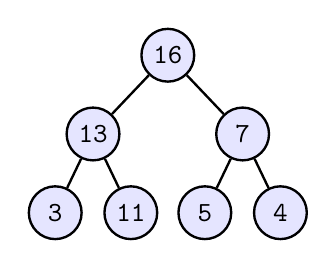
\begin{tikzpicture}

\fill[blue!10] (0.0, 0.0) circle (0.35);
\node [line width=0.03cm,black,minimum size=0.6699999999999999cm,draw,circle] at (0.0,0.0)(16){};\draw (0.0, 0.0) node[color=black] {\texttt{16}};
\fill[blue!10] (-0.95, -1.0) circle (0.35);
\node [line width=0.03cm,black,minimum size=0.6699999999999999cm,draw,circle] at (-0.95,-1.0)(13){};\draw (-0.95, -1.0) node[color=black] {\texttt{13}};
\fill[blue!10] (0.95, -1.0) circle (0.35);
\node [line width=0.03cm,black,minimum size=0.6699999999999999cm,draw,circle] at (0.95,-1.0)(7){};\draw (0.95, -1.0) node[color=black] {\texttt{7}};
\fill[blue!10] (-1.43, -2.0) circle (0.35);
\node [line width=0.03cm,black,minimum size=0.6699999999999999cm,draw,circle] at (-1.43,-2.0)(3){};\draw (-1.43, -2.0) node[color=black] {\texttt{3}};
\fill[blue!10] (-0.47, -2.0) circle (0.35);
\node [line width=0.03cm,black,minimum size=0.6699999999999999cm,draw,circle] at (-0.47,-2.0)(11){};\draw (-0.47, -2.0) node[color=black] {\texttt{11}};
\fill[blue!10] (0.47, -2.0) circle (0.35);
\node [line width=0.03cm,black,minimum size=0.6699999999999999cm,draw,circle] at (0.47,-2.0)(5){};\draw (0.47, -2.0) node[color=black] {\texttt{5}};
\fill[blue!10] (1.43, -2.0) circle (0.35);
\node [line width=0.03cm,black,minimum size=0.6699999999999999cm,draw,circle] at (1.43,-2.0)(4){};\draw (1.43, -2.0) node[color=black] {\texttt{4}};\draw[line width=0.03cm,black] (16) to  (13);
\draw[line width=0.03cm,black] (16) to  (7);
\draw[line width=0.03cm,black] (13) to  (3);
\draw[line width=0.03cm,black] (13) to  (11);
\draw[line width=0.03cm,black] (7) to  (5);
\draw[line width=0.03cm,black] (7) to  (4);
\end{tikzpicture}

\end{center}




You can merge them together to get this:

\begin{center}
\begin{tikzpicture}

\fill[blue!10] (0.0, 0.0) circle (0.35);
\node [line width=0.03cm,black,minimum size=0.6699999999999999cm,draw,circle] at (0.0,0.0)(28){};\draw (0.0, 0.0) node[color=black] {\texttt{28}};
\fill[blue!10] (-1.9, -1.0) circle (0.35);
\node [line width=0.03cm,black,minimum size=0.6699999999999999cm,draw,circle] at (-1.9,-1.0)(23){};\draw (-1.9, -1.0) node[color=black] {\texttt{23}};
\fill[blue!10] (1.9, -1.0) circle (0.35);
\node [line width=0.03cm,black,minimum size=0.6699999999999999cm,draw,circle] at (1.9,-1.0)(25){};\draw (1.9, -1.0) node[color=black] {\texttt{25}};
\fill[blue!10] (-2.85, -2.0) circle (0.35);
\node [line width=0.03cm,black,minimum size=0.6699999999999999cm,draw,circle] at (-2.85,-2.0)(10){};\draw (-2.85, -2.0) node[color=black] {\texttt{10}};
\fill[blue!10] (-0.95, -2.0) circle (0.35);
\node [line width=0.03cm,black,minimum size=0.6699999999999999cm,draw,circle] at (-0.95,-2.0)(8){};\draw (-0.95, -2.0) node[color=black] {\texttt{8}};
\fill[blue!10] (0.95, -2.0) circle (0.35);
\node [line width=0.03cm,black,minimum size=0.6699999999999999cm,draw,circle] at (0.95,-2.0)(24){};\draw (0.95, -2.0) node[color=black] {\texttt{24}};
\fill[blue!10] (2.85, -2.0) circle (0.35);
\node [line width=0.03cm,black,minimum size=0.6699999999999999cm,draw,circle] at (2.85,-2.0)(14){};\draw (2.85, -2.0) node[color=black] {\texttt{14}};
\fill[blue!10] (-3.33, -3.0) circle (0.35);
\node [line width=0.03cm,black,minimum size=0.6699999999999999cm,draw,circle] at (-3.33,-3.0)(9){};\draw (-3.33, -3.0) node[color=black] {\texttt{9}};\draw[line width=0.03cm,black] (28) to  (23);
\draw[line width=0.03cm,black] (28) to  (25);
\draw[line width=0.03cm,black] (23) to  (10);
\draw[line width=0.03cm,black] (23) to  (8);
\draw[line width=0.03cm,black] (25) to  (24);
\draw[line width=0.03cm,black] (25) to  (14);
\draw[line width=0.03cm,black] (10) to  (9);
\end{tikzpicture}

\end{center}



where \verb!99! is a fake value, i.e.,
it's 
should not be considered part of the values in
the heap container.

Of course if two heaps have very different
heights, then you won't
be able to achieve
$O(\lg n)$ runtimes for insert and delete.
For instance if the second heap from the above
has only 4 values
(i.e., \verb!16!, \verb!13!, \verb!7!, \verb!3!),
then the resulting
merged heap (using the above method)
would look like this:

\input{stdout102.tex}

%\newpage%-*-latex-*-
% https://en.wikipedia.org/wiki/Heapsort#Variations

\sectionthree{Heapsort}
\begin{python0}
from solutions import *; clear()
\end{python0}

\textsc{Heapsort given a maxheap.}
Now we delete the root from the heap.
Because this is a maxheap, the root, is the 
maximum value of \verb!x[0..9]!.
We swap \verb!x[0]! and \verb!x[9]!
and re-heapify to get a heap \verb!x[0..8]!.
In other words we're essentially doing a delete of the value at \verb!x[0]!
(the extract-max operation), putting this value at \texttt{x[9]}.

We repeat the above to get a heap \verb!x[0..7]!.
At this point the largest value of the array is at \verb!x[9]!
and the second largest is at \verb!x[8]!.

We repeat until the heap has only one value, i.e., the heap is \verb!x[0]!.
The whole array must be sorted in ascending order.

The runtime is, informally, $\log_2 n + \log_2 (n - 1) + \cdots$
which is $\log_2 n! \leq \log_2 n^n = n \log_2 n$.

So the total time for the above process,
creating the heap and then removing roots from the 
heap is roughly $2 n \log_2 n$ and therefore
the runtime for heapsort is $O(n \log_2 n)$.

Note that the heapsort has a worse runtime of $n \log_2 n$
whereas quicksort can have a worse runtime of $n^2$
although
on the average quicksort is $O(n \log n)$ and 
typically quicksort is faster than heapsort by a constant
factor.
Although mergesort does achieve $n \log_2 n$ for worse runtime,
remember that mergesort needs $O(n)$ space.
However heapsort is not stable whereas mergesort is stable.

\begin{ex}
  Give an example showing that heapsort is not
  stable.
\end{ex}
  
  

\newpage
Here is a maxheap say constructed
using build-maxheap:


\begin{center}

\begin{tikzpicture}
\node at (4,-0.8) [minimum size=8mm] (Z) {$$};
\node at (2,-1.6) [circle,draw,minimum size=8mm] (A) {$\beta$};
\node at (0,-2.4000000000000004)
    [isosceles triangle, shape border rotate=+90,
     draw,minimum size=8mm,minimum height=2cm,
     anchor=north] (Ctriangle) {$T_1$};
\coordinate (C) at (0,-2.4000000000000004);
\node at (4,-2.4000000000000004) [circle,draw,minimum size=8mm] (B) {$\alpha$};
\node at (3,-3.2)
    [isosceles triangle, shape border rotate=+90,
     draw,minimum size=8mm,minimum height=2cm,
     anchor=north] (Dtriangle) {$T_2$};
\coordinate (D) at (3,-3.2);
\node at (5,-3.2)
    [isosceles triangle, shape border rotate=+90,
     draw,minimum size=8mm,minimum height=2cm,
     anchor=north] (Etriangle) {$T_3$};
\coordinate (E) at (5,-3.2);
\draw [-,thick] (Z) -- (A);
\draw [-,thick] (A) -- (B);
\draw [-,thick] (A) -- (C);
\draw [-,thick] (B) -- (D);
\draw [-,thick] (B) -- (E);

;
\end{tikzpicture}
    
\end{center}


Let's perform heapsort on this maxheap.
Recall that extract-root will throw away the root by replacing
the value at the root with the last value in the tree (i.e.,
the rightmost value at the last level of the tree).
Instead of replacing the root with the last value,
I will \textit{swap} the root value and last value.
Otherwise it's the same extract-root operation.
Let's do it.


\textsc{Step 1}.
First I swap the root value and the last value:

\include{stdout63.tex}

x,y = pos[9]; p += Graph.node(x=x, y=y, r=BinTree.node_width, background='red!10', label='9')
p += Graph.edge(names=[7,9], linecolor='white', linewidth=0.1)
p += Graph.edge(names=[7,9], linestyle='dashed')

print(p)

I color \texttt{9} in red to remind myself
that the \texttt{9} should not be considered part of the maxheap,
but of course it's in the array.
In terms of an array the above diagram would correspond to this array:

\begin{center}
\begin{tikzpicture}

\fill[white] (5.0, 0.0) circle (0.3);
\node [draw=none,line width=0cm,black,minimum size=0.6cm,circle] at (5.0,0.0)(X){};
\fill[white] (17.0, 0.0) circle (0.3);
\node [draw=none,line width=0cm,black,minimum size=0.6cm,circle] at (17.0,0.0)(Y){};
\fill[white] (11.0, 0.0) circle (0.3);
\node [line width=0.03cm,black,minimum size=0.57cm,draw,circle] at (11.0,0.0)(a){};\draw (11.0, 0.0) node[color=black] {\texttt{18}};
\fill[white] (9.0, -1.0) circle (0.3);
\node [line width=0.03cm,black,minimum size=0.57cm,draw,circle] at (9.0,-1.0)(b){};\draw (9.0, -1.0) node[color=black] {\texttt{10}};
\fill[white] (14.0, -2.0) circle (0.3);
\node [line width=0.03cm,black,minimum size=0.57cm,draw,circle] at (14.0,-2.0)(d){};\draw (14.0, -2.0) node[color=black] {\texttt{20}};
\fill[white] (8.0, -2.0) circle (0.3);
\node [line width=0.03cm,black,minimum size=0.57cm,draw,circle] at (8.0,-2.0)(e){};\draw (8.0, -2.0) node[color=black] {\texttt{4}};
\fill[white] (12.0, -2.0) circle (0.3);
\node [line width=0.03cm,black,minimum size=0.57cm,draw,circle] at (12.0,-2.0)(f){};\draw (12.0, -2.0) node[color=black] {\texttt{19}};
\fill[white] (8.0, -4.0) circle (0.3);
\node [line width=0.03cm,black,minimum size=0.57cm,draw,circle] at (8.0,-4.0)(k){};\draw (8.0, -4.0) node[color=black] {\texttt{3}};
\fill[white] (7.0, -3.0) circle (0.3);
\node [line width=0.03cm,black,minimum size=0.57cm,draw,circle] at (7.0,-3.0)(l){};\draw (7.0, -3.0) node[color=black] {\texttt{2}};
\fill[white] (13.0, -1.0) circle (0.3);
\node [line width=0.03cm,black,minimum size=0.57cm,draw,circle] at (13.0,-1.0)(p){};\draw (13.0, -1.0) node[color=black] {\texttt{26}};
\fill[white] (6.0, -4.0) circle (0.3);
\node [line width=0.03cm,black,minimum size=0.57cm,draw,circle] at (6.0,-4.0)(n){};\draw (6.0, -4.0) node[color=black] {\texttt{0}};
\fill[white] (10.0, -2.0) circle (0.3);
\node [line width=0.03cm,black,minimum size=0.57cm,draw,circle] at (10.0,-2.0)(q){};\draw (10.0, -2.0) node[color=black] {\texttt{17}};\draw[line width=0.03cm,black,->,>=triangle 60] (e) to  (l);
\draw[line width=0.03cm,black,->,>=triangle 60] (p) to  (d);
\draw[line width=0.03cm,black,->,>=triangle 60] (b) to  (q);
\draw[line width=0.03cm,black,->,>=triangle 60] (l) to  (n);
\draw[line width=0.03cm,black,->,>=triangle 60] (l) to  (k);
\draw[line width=0.03cm,black,->,>=triangle 60] (p) to  (f);
\draw[line width=0.03cm,black,->,>=triangle 60] (a) to  (p);
\draw[line width=0.03cm,black,->,>=triangle 60] (a) to  (b);
\draw[line width=0.03cm,black,->,>=triangle 60] (b) to  (e);
\end{tikzpicture}

\end{center}



I still need to heapify-down the \texttt{6} to get this:

\begin{center}
\begin{tikzpicture}

\fill[white] (5.0, 0.0) circle (0.3);
\node [draw=none,line width=0cm,black,minimum size=0.6cm,circle] at (5.0,0.0)(X){};
\fill[white] (17.0, 0.0) circle (0.3);
\node [draw=none,line width=0cm,black,minimum size=0.6cm,circle] at (17.0,0.0)(Y){};
\fill[white] (13.0, -1.0) circle (0.3);
\node [line width=0.03cm,black,minimum size=0.57cm,draw,circle] at (13.0,-1.0)(a){};\draw (13.0, -1.0) node[color=black] {\texttt{10}};
\fill[white] (11.0, 0.0) circle (0.3);
\node [line width=0.03cm,black,minimum size=0.57cm,draw,circle] at (11.0,0.0)(b){};\draw (11.0, 0.0) node[color=black] {\texttt{4}};
\fill[white] (15.0, -3.0) circle (0.3);
\node [line width=0.03cm,black,minimum size=0.57cm,draw,circle] at (15.0,-3.0)(d){};\draw (15.0, -3.0) node[color=black] {\texttt{20}};
\fill[white] (9.0, -1.0) circle (0.3);
\node [line width=0.03cm,black,minimum size=0.57cm,draw,circle] at (9.0,-1.0)(e){};\draw (9.0, -1.0) node[color=black] {\texttt{2}};
\fill[white] (13.0, -3.0) circle (0.3);
\node [line width=0.03cm,black,minimum size=0.57cm,draw,circle] at (13.0,-3.0)(f){};\draw (13.0, -3.0) node[color=black] {\texttt{17}};
\fill[white] (8.0, -2.0) circle (0.3);
\node [line width=0.03cm,black,minimum size=0.57cm,draw,circle] at (8.0,-2.0)(k){};\draw (8.0, -2.0) node[color=black] {\texttt{0}};
\fill[white] (10.0, -2.0) circle (0.3);
\node [line width=0.03cm,black,minimum size=0.57cm,draw,circle] at (10.0,-2.0)(l){};\draw (10.0, -2.0) node[color=black] {\texttt{3}};
\fill[white] (14.0, -2.0) circle (0.3);
\node [line width=0.03cm,black,minimum size=0.57cm,draw,circle] at (14.0,-2.0)(p){};\draw (14.0, -2.0) node[color=black] {\texttt{18}};
\fill[white] (14.0, -4.0) circle (0.3);
\node [line width=0.03cm,black,minimum size=0.57cm,draw,circle] at (14.0,-4.0)(h){};\draw (14.0, -4.0) node[color=black] {\texttt{19}};
\fill[white] (16.0, -4.0) circle (0.3);
\node [line width=0.03cm,black,minimum size=0.57cm,draw,circle] at (16.0,-4.0)(m){};\draw (16.0, -4.0) node[color=black] {\texttt{26}};\draw[line width=0.03cm,black,->,>=triangle 60] (b) to  (a);
\draw[line width=0.03cm,black,->,>=triangle 60] (p) to  (f);
\draw[line width=0.03cm,black,->,>=triangle 60] (p) to  (d);
\draw[line width=0.03cm,black,->,>=triangle 60] (a) to  (p);
\draw[line width=0.03cm,black,->,>=triangle 60] (b) to  (e);
\draw[line width=0.03cm,black,->,>=triangle 60] (e) to  (k);
\draw[line width=0.03cm,black,->,>=triangle 60] (e) to  (l);
\draw[line width=0.03cm,black,->,>=triangle 60] (d) to  (h);
\draw[line width=0.03cm,black,->,>=triangle 60] (d) to  (m);
\end{tikzpicture}

\end{center}


\include{stdout66.tex}

Because I started with a maxheap, \verb!9!, the value I get from extract-root,
is the largest value in the array.
Since it moved to the last index position in the array,
this means that \verb!9! has found its right place.


\textsc{Step 2}.
Now I repeat the above process:
first I swap the root (i.e., \texttt{8}) and
the last value of the tree (i.e., \texttt{0}) to get this:


\begin{center}
\begin{tikzpicture}

\fill[white] (0.0, 0.0) circle (0.3);
\node [line width=0.03cm,black,minimum size=0.57cm,draw,circle] at (0.0,0.0)(14){};\draw (0.0, 0.0) node[color=black] {\texttt{14}};
\fill[white] (-3.2, -1.0) circle (0.3);
\node [line width=0.03cm,black,minimum size=0.57cm,draw,circle] at (-3.2,-1.0)(9){};\draw (-3.2, -1.0) node[color=black] {\texttt{9}};
\fill[white] (3.2, -1.0) circle (0.3);
\node [line width=0.03cm,black,minimum size=0.57cm,draw,circle] at (3.2,-1.0)(18){};\draw (3.2, -1.0) node[color=black] {\texttt{18}};
\fill[white] (-4.8, -2.0) circle (0.3);
\node [line width=0.03cm,black,minimum size=0.57cm,draw,circle] at (-4.8,-2.0)(5){};\draw (-4.8, -2.0) node[color=black] {\texttt{5}};
\fill[white] (-1.6, -2.0) circle (0.3);
\node [line width=0.03cm,black,minimum size=0.57cm,draw,circle] at (-1.6,-2.0)(13){};\draw (-1.6, -2.0) node[color=black] {\texttt{13}};
\fill[white] (1.6, -2.0) circle (0.3);
\node [line width=0.03cm,black,minimum size=0.57cm,draw,circle] at (1.6,-2.0)(15){};\draw (1.6, -2.0) node[color=black] {\texttt{15}};
\fill[white] (4.8, -2.0) circle (0.3);
\node [line width=0.03cm,black,minimum size=0.57cm,draw,circle] at (4.8,-2.0)(22){};\draw (4.8, -2.0) node[color=black] {\texttt{22}};
\fill[white] (-5.6, -3.0) circle (0.3);
\node [line width=0.03cm,black,minimum size=0.57cm,draw,circle] at (-5.6,-3.0)(0){};\draw (-5.6, -3.0) node[color=black] {\texttt{0}};
\fill[white] (-4.0, -3.0) circle (0.3);
\node [line width=0.03cm,black,minimum size=0.57cm,draw,circle] at (-4.0,-3.0)(8){};\draw (-4.0, -3.0) node[color=black] {\texttt{8}};
\fill[white] (-2.4, -3.0) circle (0.3);
\node [line width=0.03cm,black,minimum size=0.57cm,draw,circle] at (-2.4,-3.0)(10){};\draw (-2.4, -3.0) node[color=black] {\texttt{10}};
\fill[white] (4.0, -3.0) circle (0.3);
\node [line width=0.03cm,black,minimum size=0.57cm,draw,circle] at (4.0,-3.0)(21){};\draw (4.0, -3.0) node[color=black] {\texttt{21}};
\fill[white] (5.6, -3.0) circle (0.3);
\node [line width=0.03cm,black,minimum size=0.57cm,draw,circle] at (5.6,-3.0)(31){};\draw (5.6, -3.0) node[color=black] {\texttt{31}};
\fill[white] (-4.4, -4.0) circle (0.3);
\node [line width=0.03cm,black,minimum size=0.57cm,draw,circle] at (-4.4,-4.0)(7){};\draw (-4.4, -4.0) node[color=black] {\texttt{7}};
\fill[white] (-2.0, -4.0) circle (0.3);
\node [line width=0.03cm,black,minimum size=0.57cm,draw,circle] at (-2.0,-4.0)(11){};\draw (-2.0, -4.0) node[color=black] {\texttt{11}};
\fill[white] (3.6, -4.0) circle (0.3);
\node [line width=0.03cm,black,minimum size=0.57cm,draw,circle] at (3.6,-4.0)(19){};\draw (3.6, -4.0) node[color=black] {\texttt{19}};\draw[line width=0.03cm,black,->,>=triangle 60] (14) to  (9);
\draw[line width=0.03cm,black,->,>=triangle 60] (14) to  (18);
\draw[line width=0.03cm,black,->,>=triangle 60] (9) to  (5);
\draw[line width=0.03cm,black,->,>=triangle 60] (9) to  (13);
\draw[line width=0.03cm,black,->,>=triangle 60] (18) to  (15);
\draw[line width=0.03cm,black,->,>=triangle 60] (18) to  (22);
\draw[line width=0.03cm,black,->,>=triangle 60] (5) to  (0);
\draw[line width=0.03cm,black,->,>=triangle 60] (5) to  (8);
\draw[line width=0.03cm,black,->,>=triangle 60] (13) to  (10);
\draw[line width=0.03cm,black,->,>=triangle 60] (22) to  (21);
\draw[line width=0.03cm,black,->,>=triangle 60] (22) to  (31);
\draw[line width=0.03cm,black,->,>=triangle 60] (8) to  (7);
\draw[line width=0.03cm,black,->,>=triangle 60] (10) to  (11);
\draw[line width=0.03cm,black,->,>=triangle 60] (21) to  (19);
\end{tikzpicture}

\end{center}


\begin{center}
\begin{tikzpicture}

\draw (0.3, -0.3)
  node[draw, line width=0.04cm, , color=black,
       rounded corners=0cm, inner sep=0cm] {

\begin{minipage}[t][0.6cm]{0.6cm}
\mbox{}

\end{minipage}

};\draw (0.3, -0.3) node[color=black] {{\texttt{0}}};
\draw (0.8999999999999999, -0.3)
  node[draw, line width=0.04cm, , color=black,
       rounded corners=0cm, inner sep=0cm] {

\begin{minipage}[t][0.6cm]{0.6cm}
\mbox{}

\end{minipage}

};\draw (0.8999999999999999, -0.3) node[color=black] {{\texttt{7}}};
\draw (1.5, -0.3)
  node[draw, line width=0.04cm, , color=black,
       rounded corners=0cm, inner sep=0cm] {

\begin{minipage}[t][0.6cm]{0.6cm}
\mbox{}

\end{minipage}

};\draw (1.5, -0.3) node[color=black] {{\texttt{4}}};
\draw (2.0999999999999996, -0.3)
  node[draw, line width=0.04cm, , color=black,
       rounded corners=0cm, inner sep=0cm] {

\begin{minipage}[t][0.6cm]{0.6cm}
\mbox{}

\end{minipage}

};\draw (2.0999999999999996, -0.3) node[color=black] {{\texttt{6}}};
\draw (2.7, -0.3)
  node[draw, line width=0.04cm, , color=black,
       rounded corners=0cm, inner sep=0cm] {

\begin{minipage}[t][0.6cm]{0.6cm}
\mbox{}

\end{minipage}

};\draw (2.7, -0.3) node[color=black] {{\texttt{3}}};
\draw (3.3, -0.3)
  node[draw, line width=0.04cm, , color=black,
       rounded corners=0cm, inner sep=0cm] {

\begin{minipage}[t][0.6cm]{0.6cm}
\mbox{}

\end{minipage}

};\draw (3.3, -0.3) node[color=black] {{\texttt{2}}};
\draw (3.9, -0.3)
  node[draw, line width=0.04cm, , color=black,
       rounded corners=0cm, inner sep=0cm] {

\begin{minipage}[t][0.6cm]{0.6cm}
\mbox{}

\end{minipage}

};\draw (3.9, -0.3) node[color=black] {{\texttt{1}}};
\draw (4.5, -0.3)
  node[draw, line width=0.04cm, , color=black,
       rounded corners=0cm, inner sep=0cm] {

\begin{minipage}[t][0.6cm]{0.6cm}
\mbox{}

\end{minipage}

};\draw (4.5, -0.3) node[color=black] {{\texttt{8}}};
\draw (5.1, -0.3)
  node[draw, line width=0.04cm, , color=black,
       rounded corners=0cm, inner sep=0cm] {

\begin{minipage}[t][0.6cm]{0.6cm}
\mbox{}

\end{minipage}

};\draw (5.1, -0.3) node[color=black] {{\texttt{9}}};\draw[line width=0.1cm,black] (4.22,-0.82) to  (4.22,0.22);

\draw (1.0, -1.0)
  node[draw=none, line width=0cm, , color=black,
       rounded corners=0cm, inner sep=0cm] {

\begin{minipage}[t][0.1cm]{2cm}
\mbox{}

\end{minipage}

};
\draw (1.0, -1.0) node[color=black,
 inner sep=0cm] {
 
\begin{minipage}[t][0.1cm]{2cm}
\texttt{len = 8}
\end{minipage}

};
\end{tikzpicture}

\end{center}



(at this point \verb!9! and \verb!8! are not part of the heap)
then I heapify-down \texttt{0} to get this:

\begin{center}
\begin{tikzpicture}

\fill[white] (0.0, 0.0) circle (0.3);
\node [line width=0.03cm,black,minimum size=0.57cm,draw,circle] at (0.0,0.0)(10){};\draw (0.0, 0.0) node[color=black] {\texttt{10}};
\fill[white] (-3.0, -1.0) circle (0.3);
\node [line width=0.03cm,black,minimum size=0.57cm,draw,circle] at (-3.0,-1.0)(2){};\draw (-3.0, -1.0) node[color=black] {\texttt{2}};
\fill[white] (3.0, -1.0) circle (0.3);
\node [line width=0.03cm,black,minimum size=0.57cm,draw,circle] at (3.0,-1.0)(18){};\draw (3.0, -1.0) node[color=black] {\texttt{18}};
\fill[white] (-4.5, -2.0) circle (0.3);
\node [line width=0.03cm,black,minimum size=0.57cm,draw,circle] at (-4.5,-2.0)(0){};\draw (-4.5, -2.0) node[color=black] {\texttt{0}};
\fill[white] (-1.5, -2.0) circle (0.3);
\node [line width=0.03cm,black,minimum size=0.57cm,draw,circle] at (-1.5,-2.0)(4){};\draw (-1.5, -2.0) node[color=black] {\texttt{4}};
\fill[white] (1.5, -2.0) circle (0.3);
\node [line width=0.03cm,black,minimum size=0.57cm,draw,circle] at (1.5,-2.0)(17){};\draw (1.5, -2.0) node[color=black] {\texttt{17}};
\fill[white] (4.5, -2.0) circle (0.3);
\node [line width=0.03cm,black,minimum size=0.57cm,draw,circle] at (4.5,-2.0)(20){};\draw (4.5, -2.0) node[color=black] {\texttt{20}};
\fill[white] (-2.25, -3.0) circle (0.3);
\node [line width=0.03cm,black,minimum size=0.57cm,draw,circle] at (-2.25,-3.0)(3){};\draw (-2.25, -3.0) node[color=black] {\texttt{3}};\draw[line width=0.03cm,black,->,>=triangle 60] (10) to  (2);
\draw[line width=0.03cm,black,->,>=triangle 60] (10) to  (18);
\draw[line width=0.03cm,black,->,>=triangle 60] (4) to  (3);
\draw[line width=0.03cm,black,->,>=triangle 60] (2) to  (0);
\draw[line width=0.03cm,black,->,>=triangle 60] (2) to  (4);
\draw[line width=0.03cm,black,->,>=triangle 60] (18) to  (17);
\draw[line width=0.03cm,black,->,>=triangle 60] (18) to  (20);
\end{tikzpicture}

\end{center}



The array is


\begin{center}

\begin{tikzpicture}
\node at (3,-0.8) [minimum size=8mm] (E) {$$};
\node at (2,-2.4000000000000004) [circle,draw,minimum size=8mm] (A) {$\alpha$};
\node at (0,-3.2)
    [isosceles triangle, shape border rotate=+90,
     draw,minimum size=8mm,minimum height=2cm,
     anchor=north] (Ctriangle) {$T_1$};
\coordinate (C) at (0,-3.2);
\node at (4,-3.2)
    [isosceles triangle, shape border rotate=+90,
     draw,minimum size=8mm,minimum height=2cm,
     anchor=north] (Btriangle) {$T_2$};
\coordinate (B) at (4,-3.2);
\draw [-,thick] (A) -- (B);
\draw [-,thick] (A) -- (C);
\draw [-,thick] (E) -- (A);

;
\end{tikzpicture}
    
\end{center}



This is the second extract-max.
This means that \verb!8! is the second largest value in the array.
Note also that it's in its right place.


\textsc{Step 3}.
Next I swap the root value (i.e., \texttt{7}) and the last value
of the tree (i.e., \texttt{1})

\include{stdout71.tex}
from latextool_basic import *
p = Plot()
xs = [1, 6, 4, 0, 3, 2, 7, 8, 9]
edges = array_to_edges(xs)
pos = drawheap(p, edges, include_array=False)

x,y = pos[9]; p += Graph.node(x=x, y=y, r=BinTree.node_width, background='red!10', label='9')
x,y = pos[8]; p += Graph.node(x=x, y=y, r=BinTree.node_width, background='red!10', label='8')
x,y = pos[7]; p += Graph.node(x=x, y=y, r=BinTree.node_width, background='red!10', label='7')

p += Graph.edge(names=[0,9], linecolor='white', linewidth=0.1); p += Graph.edge(names=[0,9], linestyle='dashed')
p += Graph.edge(names=[0,8], linecolor='white', linewidth=0.1); p += Graph.edge(names=[0,8], linestyle='dashed')
p += Graph.edge(names=[4,7], linecolor='white', linewidth=0.1); p += Graph.edge(names=[4,7], linestyle='dashed')

print(p)

and heapify at \texttt{1} to get this:


\begin{center}

\begin{tikzpicture}
\node at (4,-0.8) [minimum size=8mm] (E) {$$};
\node at (3,-2.4000000000000004) [circle,draw,minimum size=8mm] (A) {$\alpha$};
\node at (1,-3.2) [circle,draw,minimum size=8mm] (C) {$\beta$};
\node at (5,-3.2)
    [isosceles triangle, shape border rotate=+90,
     draw,minimum size=8mm,
     anchor=north] (Btriangle) {$T'_3$};
\coordinate (B) at (5,-3.2);
\node at (0,-4.0)
    [isosceles triangle, shape border rotate=+90,
     draw,minimum size=8mm,
     anchor=north] (Dtriangle) {$T'_1$};
\coordinate (D) at (0,-4.0);
\node at (2,-4.0)
    [isosceles triangle, shape border rotate=+90,
     draw,minimum size=8mm,
     anchor=north] (Ftriangle) {$T'_2$};
\coordinate (F) at (2,-4.0);
\draw [-,thick] (A) -- (B);
\draw [-,thick] (A) -- (C);
\draw [-,thick] (E) -- (A);
\draw [-,thick] (C) -- (D);
\draw [-,thick] (C) -- (F);

;
\end{tikzpicture}
    
\end{center}


from latextool_basic import *
p = Plot()
xs = [6, 3, 4, 0, 1, 2, 7, 8, 9]
edges = array_to_edges(xs)
pos = drawheap(p, edges, include_array=False)

x,y = pos[9]; p += Graph.node(x=x, y=y, r=BinTree.node_width, background='red!10', label='9')
x,y = pos[8]; p += Graph.node(x=x, y=y, r=BinTree.node_width, background='red!10', label='8')
x,y = pos[7]; p += Graph.node(x=x, y=y, r=BinTree.node_width, background='red!10', label='7')

p += Graph.edge(names=[0,9], linecolor='white', linewidth=0.1); p += Graph.edge(names=[0,9], linestyle='dashed')
p += Graph.edge(names=[0,8], linecolor='white', linewidth=0.1); p += Graph.edge(names=[0,8], linestyle='dashed')
p += Graph.edge(names=[4,7], linecolor='white', linewidth=0.1); p += Graph.edge(names=[4,7], linestyle='dashed')

print(p)
\include{stdout73.tex}
from latextool_basic import *
p = Plot()
a = Array2d(0, 0, width=0.6, height=0.6, 
             xs=[['6','3', '4','0','1','2','7','8','9']])
p += a
p0 = a[0][5].bottomright(); p0 = (p0[0], p0[1] - 0.2)
p1 = a[0][5].topright(); p1 = (p1[0], p1[1] + 0.2)
p += Line(points=[p0, p1], linewidth=0.1)
p += Rect(x0=0, y0=-1, x1=2, y1=-1, s=r'\texttt{len = 6}', linewidth=0) 
print(p)

\textsc{Step 4}.
I swap \texttt{6} and \texttt{2}:

\include{stdout74.tex}
from latextool_basic import *
from drawheap import *
p = Plot()
xs = [2, 3, 4, 0, 1, 6, 7, 8, 9]
edges = array_to_edges(xs)
pos = drawheap(p, edges, include_array=False)

x,y = pos[9]; p += Graph.node(x=x, y=y, r=BinTree.node_width, background='red!10', label='9')
x,y = pos[8]; p += Graph.node(x=x, y=y, r=BinTree.node_width, background='red!10', label='8')
x,y = pos[7]; p += Graph.node(x=x, y=y, r=BinTree.node_width, background='red!10', label='7')
x,y = pos[6]; p += Graph.node(x=x, y=y, r=BinTree.node_width, background='red!10', label='6')

p += Graph.edge(names=[0,9], linecolor='white', linewidth=0.1); p += Graph.edge(names=[0,9], linestyle='dashed')
p += Graph.edge(names=[0,8], linecolor='white', linewidth=0.1); p += Graph.edge(names=[0,8], linestyle='dashed')
p += Graph.edge(names=[4,7], linecolor='white', linewidth=0.1); p += Graph.edge(names=[4,7], linestyle='dashed')
p += Graph.edge(names=[4,6], linecolor='white', linewidth=0.1); p += Graph.edge(names=[4,6], linestyle='dashed')

print(p)

and heapify-down at \texttt{2} to get:

\include{stdout75.tex}
from latextool_basic import *
p = Plot()
xs = [4, 3, 2, 0, 1, 6, 7, 8, 9]
edges = array_to_edges(xs)
pos = drawheap(p, edges, include_array=False)

x,y = pos[9]; p += Graph.node(x=x, y=y, r=BinTree.node_width, background='red!10', label='9')
x,y = pos[8]; p += Graph.node(x=x, y=y, r=BinTree.node_width, background='red!10', label='8')
x,y = pos[7]; p += Graph.node(x=x, y=y, r=BinTree.node_width, background='red!10', label='7')
x,y = pos[6]; p += Graph.node(x=x, y=y, r=BinTree.node_width, background='red!10', label='6')

p += Graph.edge(names=[0,9], linecolor='white', linewidth=0.1); p += Graph.edge(names=[0,9], linestyle='dashed')
p += Graph.edge(names=[0,8], linecolor='white', linewidth=0.1); p += Graph.edge(names=[0,8], linestyle='dashed')
p += Graph.edge(names=[2,7], linecolor='white', linewidth=0.1); p += Graph.edge(names=[2,7], linestyle='dashed')
p += Graph.edge(names=[2,6], linecolor='white', linewidth=0.1); p += Graph.edge(names=[2,6], linestyle='dashed')

print(p)
\include{stdout76.tex}
from latextool_basic import *
p = Plot()
a = Array2d(0, 0, width=0.6, height=0.6, 
             xs=[['4','3','2','0','1','6','7','8','9']])
p += a
p0 = a[0][4].bottomright(); p0 = (p0[0], p0[1] - 0.2)
p1 = a[0][4].topright(); p1 = (p1[0], p1[1] + 0.2)
p += Line(points=[p0, p1], linewidth=0.1)
p += Rect(x0=0, y0=-1, x1=2, y1=-1, s=r'\texttt{len = 5}', linewidth=0) 
print(p)


\textsc{Step 5}.
I swap \texttt{4} and \texttt{1}:

\include{stdout77.tex}
from latextool_basic import *
p = Plot()
xs = [1, 3, 2, 0, 4, 6, 7, 8, 9]
edges = array_to_edges(xs)
pos = drawheap(p, edges, include_array=False)

x,y = pos[9]; p += Graph.node(x=x, y=y, r=BinTree.node_width, background='red!10', label='9')
x,y = pos[8]; p += Graph.node(x=x, y=y, r=BinTree.node_width, background='red!10', label='8')
x,y = pos[7]; p += Graph.node(x=x, y=y, r=BinTree.node_width, background='red!10', label='7')
x,y = pos[6]; p += Graph.node(x=x, y=y, r=BinTree.node_width, background='red!10', label='6')
x,y = pos[4]; p += Graph.node(x=x, y=y, r=BinTree.node_width, background='red!10', label='4')

p += Graph.edge(names=[0,9], linecolor='white', linewidth=0.1); p += Graph.edge(names=[0,9], linestyle='dashed')
p += Graph.edge(names=[0,8], linecolor='white', linewidth=0.1); p += Graph.edge(names=[0,8], linestyle='dashed')
p += Graph.edge(names=[2,7], linecolor='white', linewidth=0.1); p += Graph.edge(names=[2,7], linestyle='dashed')
p += Graph.edge(names=[2,6], linecolor='white', linewidth=0.1); p += Graph.edge(names=[2,6], linestyle='dashed')
p += Graph.edge(names=[3,4], linecolor='white', linewidth=0.1); p += Graph.edge(names=[3,4], linestyle='dashed')

print(p)

and heapify-down at \texttt{1} to get this:


\begin{center}

\begin{tikzpicture}
\node at (3,-0.8) [minimum size=8mm] (E) {$$};
\node at (2,-2.4000000000000004) [circle,draw,minimum size=8mm] (C) {$\beta$};
\node at (0,-3.2)
    [isosceles triangle, shape border rotate=+90,
     draw,minimum size=8mm,
     anchor=north] (Dtriangle) {$T'_1$};
\coordinate (D) at (0,-3.2);
\node at (4,-3.2) [circle,draw,minimum size=8mm] (A) {$\alpha$};
\node at (2,-4.0)
    [isosceles triangle, shape border rotate=+90,
     draw,minimum size=8mm,
     anchor=north] (Ftriangle) {$T'_2+k$};
\coordinate (F) at (2,-4.0);
\node at (6,-4.0)
    [isosceles triangle, shape border rotate=+90,
     draw,minimum size=8mm,
     anchor=north] (Btriangle) {$T'_3$};
\coordinate (B) at (6,-4.0);
\draw [-,thick] (E) -- (C);
\draw [-,thick] (C) -- (D);
\draw [-,thick] (C) -- (A);
\draw [-,thick] (A) -- (F);
\draw [-,thick] (A) -- (B);

;
\end{tikzpicture}
    
\end{center}


from latextool_basic import *
p = Plot()
xs = [3, 1, 2, 0, 4, 6, 7, 8, 9]
edges = array_to_edges(xs)
pos = drawheap(p, edges, include_array=False)

x,y = pos[9]; p += Graph.node(x=x, y=y, r=BinTree.node_width, background='red!10', label='9')
x,y = pos[8]; p += Graph.node(x=x, y=y, r=BinTree.node_width, background='red!10', label='8')
x,y = pos[7]; p += Graph.node(x=x, y=y, r=BinTree.node_width, background='red!10', label='7')
x,y = pos[6]; p += Graph.node(x=x, y=y, r=BinTree.node_width, background='red!10', label='6')
x,y = pos[4]; p += Graph.node(x=x, y=y, r=BinTree.node_width, background='red!10', label='4')

p += Graph.edge(names=[0,9], linecolor='white', linewidth=0.1); p += Graph.edge(names=[0,9], linestyle='dashed')
p += Graph.edge(names=[0,8], linecolor='white', linewidth=0.1); p += Graph.edge(names=[0,8], linestyle='dashed')
p += Graph.edge(names=[2,7], linecolor='white', linewidth=0.1); p += Graph.edge(names=[2,7], linestyle='dashed')
p += Graph.edge(names=[2,6], linecolor='white', linewidth=0.1); p += Graph.edge(names=[2,6], linestyle='dashed')
p += Graph.edge(names=[1,4], linecolor='white', linewidth=0.1); p += Graph.edge(names=[1,4], linestyle='dashed')

print(p)

\begin{center}

\begin{tikzpicture}
\node at (5,-0.8) [minimum size=8mm] (E) {$$};
\node at (4,-2.4000000000000004) [circle,draw,minimum size=8mm] (A) {$\alpha$};
\node at (2,-3.2) [circle,draw,minimum size=8mm] (C) {$\beta$};
\node at (6,-3.2)
    [isosceles triangle, shape border rotate=+90,
     draw,minimum size=8mm,
     anchor=north] (Btriangle) {$T''_4$};
\coordinate (B) at (6,-3.2);
\node at (0,-4.0)
    [isosceles triangle, shape border rotate=+90,
     draw,minimum size=8mm,
     anchor=north] (Dtriangle) {$T''_1$};
\coordinate (D) at (0,-4.0);
\node at (3,-4.0) [circle,draw,minimum size=8mm] (F) {$\gamma$};
\node at (2,-4.800000000000001)
    [isosceles triangle, shape border rotate=+90,
     draw,minimum size=8mm,
     anchor=north] (Gtriangle) {$T''_2$};
\coordinate (G) at (2,-4.800000000000001);
\node at (4,-4.800000000000001)
    [isosceles triangle, shape border rotate=+90,
     draw,minimum size=8mm,
     anchor=north] (Htriangle) {$T''_3$};
\coordinate (H) at (4,-4.800000000000001);
\draw [-,thick] (A) -- (B);
\draw [-,thick] (A) -- (C);
\draw [-,thick] (E) -- (A);
\draw [-,thick] (C) -- (D);
\draw [-,thick] (C) -- (F);
\draw [-,thick] (F) -- (G);
\draw [-,thick] (F) -- (H);

;
\end{tikzpicture}
    
\end{center}


from latextool_basic import *
p = Plot()
a = Array2d(0, 0, width=0.6, height=0.6, 
             xs=[['3','1','2','0','4','6','7','8','9']])
p += a
p0 = a[0][3].bottomright(); p0 = (p0[0], p0[1] - 0.2)
p1 = a[0][3].topright(); p1 = (p1[0], p1[1] + 0.2)
p += Line(points=[p0, p1], linewidth=0.1)
p += Rect(x0=0, y0=-1, x1=2, y1=-1, s=r'\texttt{len = 4}', linewidth=0) 
print(p)


\textsc{Step 6}.
I swap \texttt{3} and \texttt{0}:


\begin{center}

\begin{tikzpicture}
\node at (7,-0.8) [minimum size=8mm] (E) {$$};
\node at (5,-2.4000000000000004) [circle,draw,minimum size=8mm] (A) {$\alpha$};
\node at (3,-3.2) [circle,draw,minimum size=8mm] (F) {$\gamma$};
\node at (7,-3.2)
    [isosceles triangle, shape border rotate=+90,
     draw,minimum size=8mm,
     anchor=north] (Btriangle) {$T''_4$};
\coordinate (B) at (7,-3.2);
\node at (1,-4.0) [circle,draw,minimum size=8mm] (C) {$\beta$};
\node at (4,-4.0)
    [isosceles triangle, shape border rotate=+90,
     draw,minimum size=8mm,
     anchor=north] (Htriangle) {$T''_3$};
\coordinate (H) at (4,-4.0);
\node at (0,-4.800000000000001)
    [isosceles triangle, shape border rotate=+90,
     draw,minimum size=8mm,
     anchor=north] (Dtriangle) {$T''_1$};
\coordinate (D) at (0,-4.800000000000001);
\node at (2,-4.800000000000001)
    [isosceles triangle, shape border rotate=+90,
     draw,minimum size=8mm,
     anchor=north] (Gtriangle) {$T''_2$};
\coordinate (G) at (2,-4.800000000000001);
\draw [-,thick] (E) -- (A);
\draw [-,thick] (A) -- (F);
\draw [-,thick] (A) -- (B);
\draw [-,thick] (F) -- (C);
\draw [-,thick] (F) -- (H);
\draw [-,thick] (C) -- (D);
\draw [-,thick] (C) -- (G);
\draw [-,thick] (A) -- (B);

;
\end{tikzpicture}
    
\end{center}


from latextool_basic import *
p = Plot()
xs = [0, 1, 2, 3, 4, 6, 7, 8, 9]
edges = array_to_edges(xs)
pos = drawheap(p, edges, include_array=False)

x,y = pos[9]; p += Graph.node(x=x, y=y, r=BinTree.node_width, background='red!10', label='9')
x,y = pos[8]; p += Graph.node(x=x, y=y, r=BinTree.node_width, background='red!10', label='8')
x,y = pos[7]; p += Graph.node(x=x, y=y, r=BinTree.node_width, background='red!10', label='7')
x,y = pos[6]; p += Graph.node(x=x, y=y, r=BinTree.node_width, background='red!10', label='6')
x,y = pos[4]; p += Graph.node(x=x, y=y, r=BinTree.node_width, background='red!10', label='4')
x,y = pos[3]; p += Graph.node(x=x, y=y, r=BinTree.node_width, background='red!10', label='3')

p += Graph.edge(names=[3,9], linecolor='white', linewidth=0.1); p += Graph.edge(names=[3,9], linestyle='dashed')
p += Graph.edge(names=[3,8], linecolor='white', linewidth=0.1); p += Graph.edge(names=[3,8], linestyle='dashed')
p += Graph.edge(names=[2,7], linecolor='white', linewidth=0.1); p += Graph.edge(names=[2,7], linestyle='dashed')
p += Graph.edge(names=[2,6], linecolor='white', linewidth=0.1); p += Graph.edge(names=[2,6], linestyle='dashed')
p += Graph.edge(names=[1,4], linecolor='white', linewidth=0.1); p += Graph.edge(names=[1,4], linestyle='dashed')
p += Graph.edge(names=[1,3], linecolor='white', linewidth=0.1); p += Graph.edge(names=[1,3], linestyle='dashed')

print(p)

heapify-down at \texttt{0}:


\begin{center}

\begin{tikzpicture}
\node at (5,-0.8) [minimum size=8mm] (E) {$$};
\node at (3,-2.4000000000000004) [circle,draw,minimum size=8mm] (F) {$\gamma$};
\node at (1,-3.2) [circle,draw,minimum size=8mm] (C) {$\beta$};
\node at (5,-3.2) [circle,draw,minimum size=8mm] (A) {$\alpha$};
\node at (0,-4.0)
    [isosceles triangle, shape border rotate=+90,
     draw,minimum size=8mm,
     anchor=north] (Dtriangle) {$T''_1$};
\coordinate (D) at (0,-4.0);
\node at (2,-4.0)
    [isosceles triangle, shape border rotate=+90,
     draw,minimum size=8mm,
     anchor=north] (Gtriangle) {$T''_2$};
\coordinate (G) at (2,-4.0);
\node at (4,-4.0)
    [isosceles triangle, shape border rotate=+90,
     draw,minimum size=8mm,
     anchor=north] (Htriangle) {$T''_3$};
\coordinate (H) at (4,-4.0);
\node at (6,-4.0)
    [isosceles triangle, shape border rotate=+90,
     draw,minimum size=8mm,
     anchor=north] (Btriangle) {$T''_4$};
\coordinate (B) at (6,-4.0);
\draw [-,thick] (E) -- (F);
\draw [-,thick] (F) -- (C);
\draw [-,thick] (F) -- (A);
\draw [-,thick] (C) -- (D);
\draw [-,thick] (C) -- (G);
\draw [-,thick] (A) -- (H);
\draw [-,thick] (A) -- (B);

;
\end{tikzpicture}
    
\end{center}


from latextool_basic import *
p = Plot()
xs = [2, 1, 0, 3, 4, 6, 7, 8, 9]
edges = array_to_edges(xs)
pos = drawheap(p, edges, include_array=False)

x,y = pos[9]; p += Graph.node(x=x, y=y, r=BinTree.node_width, background='red!10', label='9')
x,y = pos[8]; p += Graph.node(x=x, y=y, r=BinTree.node_width, background='red!10', label='8')
x,y = pos[7]; p += Graph.node(x=x, y=y, r=BinTree.node_width, background='red!10', label='7')
x,y = pos[6]; p += Graph.node(x=x, y=y, r=BinTree.node_width, background='red!10', label='6')
x,y = pos[4]; p += Graph.node(x=x, y=y, r=BinTree.node_width, background='red!10', label='4')
x,y = pos[3]; p += Graph.node(x=x, y=y, r=BinTree.node_width, background='red!10', label='3')

p += Graph.edge(names=[3,9], linecolor='white', linewidth=0.1); p += Graph.edge(names=[3,9], linestyle='dashed')
p += Graph.edge(names=[3,8], linecolor='white', linewidth=0.1); p += Graph.edge(names=[3,8], linestyle='dashed')
p += Graph.edge(names=[0,7], linecolor='white', linewidth=0.1); p += Graph.edge(names=[0,7], linestyle='dashed')
p += Graph.edge(names=[0,6], linecolor='white', linewidth=0.1); p += Graph.edge(names=[0,6], linestyle='dashed')
p += Graph.edge(names=[1,4], linecolor='white', linewidth=0.1); p += Graph.edge(names=[1,4], linestyle='dashed')
p += Graph.edge(names=[1,3], linecolor='white', linewidth=0.1); p += Graph.edge(names=[1,3], linestyle='dashed')

print(p)
\begin{center}
\begin{tikzpicture}

\fill[white] (0.0, 0.0) circle (0.3);
\node [line width=0.03cm,black,minimum size=0.57cm,draw,circle] at (0.0,0.0)(10){};\draw (0.0, 0.0) node[color=black] {\texttt{10}};
\fill[white] (-0.75, -1.0) circle (0.3);
\node [line width=0.03cm,black,minimum size=0.57cm,draw,circle] at (-0.75,-1.0)(5){};\draw (-0.75, -1.0) node[color=black] {\texttt{5}};
\fill[white] (0.75, -1.0) circle (0.3);
\node [line width=0.03cm,black,minimum size=0.57cm,draw,circle] at (0.75,-1.0)(18){};\draw (0.75, -1.0) node[color=black] {\texttt{18}};\draw[line width=0.03cm,black,->,>=triangle 60] (10) to  (5);
\draw[line width=0.03cm,black,->,>=triangle 60] (10) to  (18);
\end{tikzpicture}

\end{center}


from latextool_basic import *
p = Plot()
a = Array2d(0, 0, width=0.6, height=0.6, 
             xs=[['2','1','0','3','4','6','7','8','9']])
p += a
p0 = a[0][2].bottomright(); p0 = (p0[0], p0[1] - 0.2)
p1 = a[0][2].topright(); p1 = (p1[0], p1[1] + 0.2)
p += Line(points=[p0, p1], linewidth=0.1)
p += Rect(x0=0, y0=-1, x1=2, y1=-1, s=r'\texttt{len = 3}', linewidth=0) 
print(p)


\textsc{Step 7}.
Swap \texttt{2} and \texttt{0}:

\begin{center}
\begin{tikzpicture}

\fill[white] (0.0, 0.0) circle (0.3);
\node [line width=0.03cm,black,minimum size=0.57cm,draw,circle] at (0.0,0.0)(10){};\draw (0.0, 0.0) node[color=black] {\texttt{10}};
\fill[white] (-1.5, -1.0) circle (0.3);
\node [line width=0.03cm,black,minimum size=0.57cm,draw,circle] at (-1.5,-1.0)(5){};\draw (-1.5, -1.0) node[color=black] {\texttt{5}};
\fill[white] (1.5, -1.0) circle (0.3);
\node [line width=0.03cm,black,minimum size=0.57cm,draw,circle] at (1.5,-1.0)(18){};\draw (1.5, -1.0) node[color=black] {\texttt{18}};
\fill[white] (-2.25, -2.0) circle (0.3);
\node [line width=0.03cm,black,minimum size=0.57cm,draw,circle] at (-2.25,-2.0)(2){};\draw (-2.25, -2.0) node[color=black] {\texttt{2}};\draw[line width=0.03cm,black,->,>=triangle 60] (10) to  (5);
\draw[line width=0.03cm,black,->,>=triangle 60] (10) to  (18);
\draw[line width=0.03cm,black,->,>=triangle 60] (5) to  (2);
\end{tikzpicture}

\end{center}


from latextool_basic import *
p = Plot()
xs = [0, 1, 2, 3, 4, 6, 7, 8, 9]
edges = array_to_edges(xs)
pos = drawheap(p, edges, include_array=False)

x,y = pos[9]; p += Graph.node(x=x, y=y, r=BinTree.node_width, background='red!10', label='9')
x,y = pos[8]; p += Graph.node(x=x, y=y, r=BinTree.node_width, background='red!10', label='8')
x,y = pos[7]; p += Graph.node(x=x, y=y, r=BinTree.node_width, background='red!10', label='7')
x,y = pos[6]; p += Graph.node(x=x, y=y, r=BinTree.node_width, background='red!10', label='6')
x,y = pos[4]; p += Graph.node(x=x, y=y, r=BinTree.node_width, background='red!10', label='4')
x,y = pos[3]; p += Graph.node(x=x, y=y, r=BinTree.node_width, background='red!10', label='3')
x,y = pos[2]; p += Graph.node(x=x, y=y, r=BinTree.node_width, background='red!10', label='2')

p += Graph.edge(names=[0,2], linecolor='white', linewidth=0.1); p += Graph.edge(names=[0,2], linestyle='dashed')
p += Graph.edge(names=[3,9], linecolor='white', linewidth=0.1); p += Graph.edge(names=[3,9], linestyle='dashed')
p += Graph.edge(names=[3,8], linecolor='white', linewidth=0.1); p += Graph.edge(names=[3,8], linestyle='dashed')
p += Graph.edge(names=[2,7], linecolor='white', linewidth=0.1); p += Graph.edge(names=[2,7], linestyle='dashed')
p += Graph.edge(names=[2,6], linecolor='white', linewidth=0.1); p += Graph.edge(names=[2,6], linestyle='dashed')
p += Graph.edge(names=[1,4], linecolor='white', linewidth=0.1); p += Graph.edge(names=[1,4], linestyle='dashed')
p += Graph.edge(names=[1,3], linecolor='white', linewidth=0.1); p += Graph.edge(names=[1,3], linestyle='dashed')

print(p)

heapify-down at \texttt{0}:

\begin{center}
\begin{tikzpicture}

\fill[blue!10] (0.0, 0.0) circle (0.35);
\node [line width=0.03cm,black,minimum size=0.6699999999999999cm,draw,circle] at (0.0,0.0)(1){};\draw (0.0, 0.0) node[color=black] {\texttt{1}};
\fill[blue!10] (-1.9, -1.0) circle (0.35);
\node [line width=0.03cm,black,minimum size=0.6699999999999999cm,draw,circle] at (-1.9,-1.0)(0){};\draw (-1.9, -1.0) node[color=black] {\texttt{0}};
\fill[blue!10] (1.9, -1.0) circle (0.35);
\node [line width=0.03cm,black,minimum size=0.6699999999999999cm,draw,circle] at (1.9,-1.0)(2){};\draw (1.9, -1.0) node[color=black] {\texttt{2}};
\fill[blue!10] (-2.85, -2.0) circle (0.35);
\node [line width=0.03cm,black,minimum size=0.6699999999999999cm,draw,circle] at (-2.85,-2.0)(3){};\draw (-2.85, -2.0) node[color=black] {\texttt{3}};
\fill[blue!10] (-0.95, -2.0) circle (0.35);
\node [line width=0.03cm,black,minimum size=0.6699999999999999cm,draw,circle] at (-0.95,-2.0)(4){};\draw (-0.95, -2.0) node[color=black] {\texttt{4}};
\fill[blue!10] (0.95, -2.0) circle (0.35);
\node [line width=0.03cm,black,minimum size=0.6699999999999999cm,draw,circle] at (0.95,-2.0)(6){};\draw (0.95, -2.0) node[color=black] {\texttt{6}};
\fill[blue!10] (2.85, -2.0) circle (0.35);
\node [line width=0.03cm,black,minimum size=0.6699999999999999cm,draw,circle] at (2.85,-2.0)(7){};\draw (2.85, -2.0) node[color=black] {\texttt{7}};
\fill[blue!10] (-3.33, -3.0) circle (0.35);
\node [line width=0.03cm,black,minimum size=0.6699999999999999cm,draw,circle] at (-3.33,-3.0)(8){};\draw (-3.33, -3.0) node[color=black] {\texttt{8}};
\fill[blue!10] (-2.38, -3.0) circle (0.35);
\node [line width=0.03cm,black,minimum size=0.6699999999999999cm,draw,circle] at (-2.38,-3.0)(9){};\draw (-2.38, -3.0) node[color=black] {\texttt{9}};\draw[line width=0.03cm,black] (1) to  (0);
\draw[line width=0.03cm,black] (1) to  (2);
\draw[line width=0.03cm,black] (0) to  (3);
\draw[line width=0.03cm,black] (0) to  (4);
\draw[line width=0.03cm,black] (2) to  (6);
\draw[line width=0.03cm,black] (2) to  (7);
\draw[line width=0.03cm,black] (3) to  (8);
\draw[line width=0.03cm,black] (3) to  (9);

\fill[red!10] (-2.38, -3.0) circle (0.35);
\draw[line width=0.03cm,black] (-2.38, -3.0) circle (0.33499999999999996);\draw (-2.38, -3.0) node[color=black] {9};
\fill[red!10] (-3.33, -3.0) circle (0.35);
\draw[line width=0.03cm,black] (-3.33, -3.0) circle (0.33499999999999996);\draw (-3.33, -3.0) node[color=black] {8};
\fill[red!10] (2.85, -2.0) circle (0.35);
\draw[line width=0.03cm,black] (2.85, -2.0) circle (0.33499999999999996);\draw (2.85, -2.0) node[color=black] {7};
\fill[red!10] (0.95, -2.0) circle (0.35);
\draw[line width=0.03cm,black] (0.95, -2.0) circle (0.33499999999999996);\draw (0.95, -2.0) node[color=black] {6};
\fill[red!10] (-0.95, -2.0) circle (0.35);
\draw[line width=0.03cm,black] (-0.95, -2.0) circle (0.33499999999999996);\draw (-0.95, -2.0) node[color=black] {4};
\fill[red!10] (-2.85, -2.0) circle (0.35);
\draw[line width=0.03cm,black] (-2.85, -2.0) circle (0.33499999999999996);\draw (-2.85, -2.0) node[color=black] {3};
\fill[red!10] (1.9, -1.0) circle (0.35);
\draw[line width=0.03cm,black] (1.9, -1.0) circle (0.33499999999999996);\draw (1.9, -1.0) node[color=black] {2};\draw[line width=0.1cm,white] (1) to  (2);
\draw[line width=0.03cm,black,,dashed] (1) to  (2);
\draw[line width=0.1cm,white] (3) to  (9);
\draw[line width=0.03cm,black,,dashed] (3) to  (9);
\draw[line width=0.1cm,white] (3) to  (8);
\draw[line width=0.03cm,black,,dashed] (3) to  (8);
\draw[line width=0.1cm,white] (2) to  (7);
\draw[line width=0.03cm,black,,dashed] (2) to  (7);
\draw[line width=0.1cm,white] (2) to  (6);
\draw[line width=0.03cm,black,,dashed] (2) to  (6);
\draw[line width=0.1cm,white] (0) to  (4);
\draw[line width=0.03cm,black,,dashed] (0) to  (4);
\draw[line width=0.1cm,white] (0) to  (3);
\draw[line width=0.03cm,black,,dashed] (0) to  (3);
\end{tikzpicture}

\end{center}


from latextool_basic import *
p = Plot()
xs = [1, 0, 2, 3, 4, 6, 7, 8, 9]
edges = array_to_edges(xs)
pos = drawheap(p, edges, include_array=False)

x,y = pos[9]; p += Graph.node(x=x, y=y, r=BinTree.node_width, background='red!10', label='9')
x,y = pos[8]; p += Graph.node(x=x, y=y, r=BinTree.node_width, background='red!10', label='8')
x,y = pos[7]; p += Graph.node(x=x, y=y, r=BinTree.node_width, background='red!10', label='7')
x,y = pos[6]; p += Graph.node(x=x, y=y, r=BinTree.node_width, background='red!10', label='6')
x,y = pos[4]; p += Graph.node(x=x, y=y, r=BinTree.node_width, background='red!10', label='4')
x,y = pos[3]; p += Graph.node(x=x, y=y, r=BinTree.node_width, background='red!10', label='3')
x,y = pos[2]; p += Graph.node(x=x, y=y, r=BinTree.node_width, background='red!10', label='2')

p += Graph.edge(names=[1,2], linecolor='white', linewidth=0.1); p += Graph.edge(names=[1,2], linestyle='dashed')
p += Graph.edge(names=[3,9], linecolor='white', linewidth=0.1); p += Graph.edge(names=[3,9], linestyle='dashed')
p += Graph.edge(names=[3,8], linecolor='white', linewidth=0.1); p += Graph.edge(names=[3,8], linestyle='dashed')
p += Graph.edge(names=[2,7], linecolor='white', linewidth=0.1); p += Graph.edge(names=[2,7], linestyle='dashed')
p += Graph.edge(names=[2,6], linecolor='white', linewidth=0.1); p += Graph.edge(names=[2,6], linestyle='dashed')
p += Graph.edge(names=[0,4], linecolor='white', linewidth=0.1); p += Graph.edge(names=[0,4], linestyle='dashed')
p += Graph.edge(names=[0,3], linecolor='white', linewidth=0.1); p += Graph.edge(names=[0,3], linestyle='dashed')

print(p)
\begin{center}
\begin{tikzpicture}

\fill[white] (0.0, 0.0) circle (0.3);
\node [line width=0.03cm,black,minimum size=0.57cm,draw,circle] at (0.0,0.0)(10){};\draw (0.0, 0.0) node[color=black] {\texttt{10}};
\fill[white] (-3.0, -1.0) circle (0.35);
\node [line width=0.1cm,red,minimum size=0.6cm,draw,circle] at (-3.0,-1.0)(5){};\draw (-3.0, -1.0) node[color=black] {\texttt{5}};
\fill[white] (3.0, -1.0) circle (0.3);
\node [line width=0.03cm,black,minimum size=0.57cm,draw,circle] at (3.0,-1.0)(18){};\draw (3.0, -1.0) node[color=black] {\texttt{18}};
\fill[white] (-4.5, -2.0) circle (0.3);
\node [line width=0.03cm,black,minimum size=0.57cm,draw,circle] at (-4.5,-2.0)(2){};\draw (-4.5, -2.0) node[color=black] {\texttt{2}};
\fill[white] (-5.25, -3.0) circle (0.3);
\node [line width=0.03cm,black,minimum size=0.57cm,draw,circle] at (-5.25,-3.0)(0){};\draw (-5.25, -3.0) node[color=black] {\texttt{0}};\draw[line width=0.03cm,black,->,>=triangle 60] (10) to  (5);
\draw[line width=0.03cm,black,->,>=triangle 60] (10) to  (18);
\draw[line width=0.1cm,red,->,>=triangle 60] (5) to  (2);
\draw[line width=0.1cm,red,->,>=triangle 60] (2) to  (0);
\end{tikzpicture}

\end{center}


from latextool_basic import *
p = Plot()
a = Array2d(0, 0, width=0.6, height=0.6, 
             xs=[['1','0','2','3','4','6','7','8','9']])
p += a
p0 = a[0][1].bottomright(); p0 = (p0[0], p0[1] - 0.2)
p1 = a[0][1].topright(); p1 = (p1[0], p1[1] + 0.2)
p += Line(points=[p0, p1], linewidth=0.1)
p += Rect(x0=0, y0=-1, x1=2, y1=-1, s=r'\texttt{len = 2}', linewidth=0) 
print(p)


\textsc{Step 8}.
I swap \texttt{1} and \texttt{0}

\begin{center}
\begin{tikzpicture}

\fill[white] (0.0, 0.0) circle (0.3);
\node [line width=0.03cm,black,minimum size=0.57cm,draw,circle] at (0.0,0.0)(10){};\draw (0.0, 0.0) node[color=black] {\texttt{10}};
\fill[white] (-1.5, -1.0) circle (0.35);
\node [line width=0.1cm,red,minimum size=0.6cm,draw,circle] at (-1.5,-1.0)(2){};\draw (-1.5, -1.0) node[color=black] {\texttt{2}};
\fill[white] (1.5, -1.0) circle (0.3);
\node [line width=0.03cm,black,minimum size=0.57cm,draw,circle] at (1.5,-1.0)(18){};\draw (1.5, -1.0) node[color=black] {\texttt{18}};
\fill[white] (-2.25, -2.0) circle (0.3);
\node [line width=0.03cm,black,minimum size=0.57cm,draw,circle] at (-2.25,-2.0)(0){};\draw (-2.25, -2.0) node[color=black] {\texttt{0}};
\fill[white] (-0.75, -2.0) circle (0.3);
\node [line width=0.03cm,black,minimum size=0.57cm,draw,circle] at (-0.75,-2.0)(5){};\draw (-0.75, -2.0) node[color=black] {\texttt{5}};\draw[line width=0.03cm,black,->,>=triangle 60] (10) to  (2);
\draw[line width=0.03cm,black,->,>=triangle 60] (10) to  (18);
\draw[line width=0.03cm,black,->,>=triangle 60] (2) to  (0);
\draw[line width=0.03cm,black,->,>=triangle 60] (2) to  (5);
\end{tikzpicture}

\end{center}


from latextool_basic import *
p = Plot()
xs = [0, 1, 2, 3, 4, 6, 7, 8, 9]
edges = array_to_edges(xs)
pos = drawheap(p, edges, include_array=False)

x,y = pos[9]; p += Graph.node(x=x, y=y, r=BinTree.node_width, background='red!10', label='9')
x,y = pos[8]; p += Graph.node(x=x, y=y, r=BinTree.node_width, background='red!10', label='8')
x,y = pos[7]; p += Graph.node(x=x, y=y, r=BinTree.node_width, background='red!10', label='7')
x,y = pos[6]; p += Graph.node(x=x, y=y, r=BinTree.node_width, background='red!10', label='6')
x,y = pos[4]; p += Graph.node(x=x, y=y, r=BinTree.node_width, background='red!10', label='4')
x,y = pos[3]; p += Graph.node(x=x, y=y, r=BinTree.node_width, background='red!10', label='3')
x,y = pos[2]; p += Graph.node(x=x, y=y, r=BinTree.node_width, background='red!10', label='2')
x,y = pos[1]; p += Graph.node(x=x, y=y, r=BinTree.node_width, background='red!10', label='1')

p += Graph.edge(names=[3,9], linecolor='white', linewidth=0.1); p += Graph.edge(names=[3,9], linestyle='dashed')
p += Graph.edge(names=[3,8], linecolor='white', linewidth=0.1); p += Graph.edge(names=[3,8], linestyle='dashed')
p += Graph.edge(names=[2,7], linecolor='white', linewidth=0.1); p += Graph.edge(names=[2,7], linestyle='dashed')
p += Graph.edge(names=[2,6], linecolor='white', linewidth=0.1); p += Graph.edge(names=[2,6], linestyle='dashed')
p += Graph.edge(names=[1,4], linecolor='white', linewidth=0.1); p += Graph.edge(names=[1,4], linestyle='dashed')
p += Graph.edge(names=[1,3], linecolor='white', linewidth=0.1); p += Graph.edge(names=[1,3], linestyle='dashed')
p += Graph.edge(names=[0,1], linecolor='white', linewidth=0.1); p += Graph.edge(names=[0,1], linestyle='dashed')
p += Graph.edge(names=[0,2], linecolor='white', linewidth=0.1); p += Graph.edge(names=[0,2], linestyle='dashed')

print(p)

Clearly there's no need to heapify-down since the tree now has size 1.
At this point, the array is
\begin{center}
\begin{tikzpicture}

\fill[white] (0.0, 0.0) circle (0.3);
\node [line width=0.03cm,black,minimum size=0.57cm,draw,circle] at (0.0,0.0)(10){};\draw (0.0, 0.0) node[color=black] {\texttt{10}};
\fill[white] (-3.0, -1.0) circle (0.3);
\node [line width=0.03cm,black,minimum size=0.57cm,draw,circle] at (-3.0,-1.0)(2){};\draw (-3.0, -1.0) node[color=black] {\texttt{2}};
\fill[white] (3.0, -1.0) circle (0.3);
\node [line width=0.03cm,black,minimum size=0.57cm,draw,circle] at (3.0,-1.0)(18){};\draw (3.0, -1.0) node[color=black] {\texttt{18}};
\fill[white] (-4.5, -2.0) circle (0.3);
\node [line width=0.03cm,black,minimum size=0.57cm,draw,circle] at (-4.5,-2.0)(0){};\draw (-4.5, -2.0) node[color=black] {\texttt{0}};
\fill[white] (-1.5, -2.0) circle (0.3);
\node [line width=0.03cm,black,minimum size=0.57cm,draw,circle] at (-1.5,-2.0)(5){};\draw (-1.5, -2.0) node[color=black] {\texttt{5}};
\fill[white] (-2.25, -3.0) circle (0.3);
\node [line width=0.03cm,black,minimum size=0.57cm,draw,circle] at (-2.25,-3.0)(3){};\draw (-2.25, -3.0) node[color=black] {\texttt{3}};\draw[line width=0.1cm,red,->,>=triangle 60] (10) to  (2);
\draw[line width=0.03cm,black,->,>=triangle 60] (10) to  (18);
\draw[line width=0.03cm,black,->,>=triangle 60] (2) to  (0);
\draw[line width=0.1cm,red,->,>=triangle 60] (2) to  (5);
\draw[line width=0.1cm,red,->,>=triangle 60] (5) to  (3);
\end{tikzpicture}

\end{center}


from latextool_basic import *
p = Plot()
a = Array2d(0, 0, width=0.6, height=0.6, 
             xs=[['0','1','2','3','4','6','7','8','9']])
p += a
p0 = a[0][0].bottomright(); p0 = (p0[0], p0[1] - 0.2)
p1 = a[0][0].topright(); p1 = (p1[0], p1[1] + 0.2)
p += Line(points=[p0, p1], linewidth=0.1)
p += Rect(x0=0, y0=-1, x1=2, y1=-1, s=r'\texttt{len = 1}', linewidth=0) 
print(p)
It's sorted!

Here's the algorithm:
\begin{console}
ALGORITHM: heapsort
INPUT:     x - array
           n - length of x

Perform build_maxheap on x[0..n - 1]
for i = n - 1, n - 2, ..., 1: 
    swap x[0] and x[i]
    perform heapify_down on x[0..i - 1] at index 0
\end{console}

\newpage
\begin{ex}
Perform heapsort on given arrays below (in ascending order).
Execute build-maxheap and then continually perform
extract-max and heapify.
Draw the tree after every extract-max and heapify and draw the
corresponding array.
\begin{tightlist}
  \li \verb![5, 7, 4, 0, 8]!
  \li \verb![3, 9, 0, 7, 2, 5, 4, 1, 0]!
  \li \verb![1, 3, 5, 7, 6, 4, 2, 0, 8, 9]!
  \li \verb![0, 1, 2, 3, 4, 5, 6, 7, 8, 9]!
  \li \verb![9, 8, 7, 6, 5, 4, 3, 2, 1, 0]!
\end{tightlist}
\end{ex}

\newpage
\begin{ex}
  Now do the same as above
  except that you perform heapsort in \textit{descending} order.
\begin{tightlist}
  \li \verb![5, 7, 4, 0, 8]!
  \li \verb![3, 9, 0, 7, 2, 5, 4, 1, 0]!
  \li \verb![1, 3, 5, 7, 6, 4, 2, 0, 8, 9]!
  \li \verb![0, 1, 2, 3, 4, 5, 6, 7, 8, 9]!
  \li \verb![9, 8, 7, 6, 5, 4, 3, 2, 1, 0]!
\end{tightlist}
\end{ex}


\newpage
\begin{ex}
An array $x$ of size $n$ represents a maxheap.
What is the fastest way to find the minimum value in $x$?
\qed
\end{ex}
% The minimum must be a leave. Look at $n/2, ..., n - 1$.
% n-1 - n/2 + 1 = n - n / 2 accesses.


\newpage
\begin{ex}
Figure out a good algorithmn to merge two maxheaps.
\qed
\end{ex}



%\newpage%-*-latex-*-
\section{Questions}

The minheap basically have pointers going to values smaller
than the root.
But there's no organization about the children.
What if the children are organized?
What if left subtree have values $\leq k$ and 
right subtree have values $> k$?
Say root is 10.
Insert 5 goes into left child first. $k$ is set fo $5$.
What happens with insert 3?
We can change the left, right pointers.
So that left points to 3, right points to 5 
and $k = 4$?
Are there such trees?
After insert 1 and 2 which will go into 3,
what if I insert 0?

What is we do lazy extract-max?
Suppose we extract-root and do not heapify and only heapify during the 
second extract-root?
What is the heapify like if we delete two roots?



\begin{python0}
from solutions import *
prepare_solutions()
\end{python0}

\newpage
\section*{Solutions}
Solution to Exercise \ref{ex:dfa0}\labeltext{}{sol:dfa0}.

\tinysidebar{\debug{exercises/{dfa0/answer.tex}}}

    Solution not provided.
    

\newpage

Solution to Exercise \ref{ex:dfa1}\labeltext{}{sol:dfa1}.

\tinysidebar{\debug{exercises/{dfa1/answer.tex}}}
  The ID computation is
  \begin{align*}
    (q_0, aba)
    &\vdash (\delta(q_0, a), ba) = (q_0, ba) \\ 
    &\vdash (\delta(q_0, b), a) = (q_1, a) \\
    &\vdash (\delta(q_1, a), \ep) = (q_0, \ep)
  \end{align*}
  $q_0$ is not an accept state. Therefore $aba$ is not accepted.


\newpage

Solution to Exercise \ref{ex:dfa4}\labeltext{}{sol:dfa4}.

\tinysidebar{\debug{exercises/{dfa4/answer.tex}}}

    Solution not provided.
    

\newpage

Solution to Exercise \ref{ex:dfa5}\labeltext{}{sol:dfa5}.

\tinysidebar{\debug{exercises/{dfa5/answer.tex}}}

    Solution not provided.
    

\newpage

Solution to Exercise \ref{ex:implementing-a-single-dfa0}\labeltext{}{sol:implementing-a-single-dfa0}.

\tinysidebar{\debug{exercises/{implementing-a-single-dfa0/answer.tex}}}

    Solution not provided.
    

\newpage

Solution to Exercise \ref{ex:nfastatediag0}\labeltext{}{sol:nfastatediag0}.

\tinysidebar{\debug{exercises/{nfastatediag0/answer.tex}}}

    Solution not provided.
    

\newpage

Solution to Exercise \ref{ex:nfastatediag1}\labeltext{}{sol:nfastatediag1}.

\tinysidebar{\debug{exercises/{nfastatediag1/answer.tex}}}

    Solution not provided.
    

\newpage

Solution to Exercise \ref{ex:nfastatediag2}\labeltext{}{sol:nfastatediag2}.

\tinysidebar{\debug{exercises/{nfastatediag2/answer.tex}}}

    Solution not provided.
    

\newpage

Solution to Exercise \ref{ex:nfastatediag3}\labeltext{}{sol:nfastatediag3}.

\tinysidebar{\debug{exercises/{nfastatediag3/answer.tex}}}

    Solution not provided.
    

\newpage

Solution to Exercise \ref{ex:nfastatediag4}\labeltext{}{sol:nfastatediag4}.

\tinysidebar{\debug{exercises/{nfastatediag4/answer.tex}}}

    Solution not provided.
    

\newpage

Solution to Exercise \ref{ex:nfastatediag5}\labeltext{}{sol:nfastatediag5}.

\tinysidebar{\debug{exercises/{nfastatediag5/answer.tex}}}

    Solution not provided.
    

\newpage

Solution to Exercise \ref{ex:nfastatediag6}\labeltext{}{sol:nfastatediag6}.

\tinysidebar{\debug{exercises/{nfastatediag6/answer.tex}}}

    Solution not provided.
    

\newpage

Solution to Exercise \ref{ex:nfastatediag7}\labeltext{}{sol:nfastatediag7}.

\tinysidebar{\debug{exercises/{nfastatediag7/answer.tex}}}

    Solution not provided.
    

\newpage

Solution to Exercise \ref{ex:nfastatediag8}\labeltext{}{sol:nfastatediag8}.

\tinysidebar{\debug{exercises/{nfastatediag8/answer.tex}}}

    Solution not provided.
    

\newpage

Solution to Exercise \ref{ex:nfastatediag9}\labeltext{}{sol:nfastatediag9}.

\tinysidebar{\debug{exercises/{nfastatediag9/answer.tex}}}

    Solution not provided.
    

\newpage

Solution to Exercise \ref{ex:nfastatediag10}\labeltext{}{sol:nfastatediag10}.

\tinysidebar{\debug{exercises/{nfastatediag10/answer.tex}}}

    Solution not provided.
    

\newpage

Solution to Exercise \ref{ex:nfastatediag11}\labeltext{}{sol:nfastatediag11}.

\tinysidebar{\debug{exercises/{nfastatediag11/answer.tex}}}

    Solution not provided.
    

\newpage

Solution to Exercise \ref{ex:nfastatediag12}\labeltext{}{sol:nfastatediag12}.

\tinysidebar{\debug{exercises/{nfastatediag12/answer.tex}}}

    Solution not provided.
    

\newpage

Solution to Exercise \ref{ex:nfastatediag13}\labeltext{}{sol:nfastatediag13}.

\tinysidebar{\debug{exercises/{nfastatediag13/answer.tex}}}

    Solution not provided.
    

\newpage

Solution to Exercise \ref{ex:nfa0}\labeltext{}{sol:nfa0}.

\tinysidebar{\debug{exercises/{nfa0/answer.tex}}}
The formal definition of this NFA is $(\Sigma, Q, q_0, \delta, F)$ where
\begin{tightlist}
\li $\Sigma = \{a,b\}$
\li $Q = \{q_0\}$
\li $\delta$ is the function
\[
\delta : Q \times \Sigma_\epsilon \rightarrow P(Q)
\]
given by
\begin{align*}
  \delta(q_0, \epsilon) &= \{\} \\
  \delta(q_0, a) &= \{\} \\
  \delta(q_0, b) &= \{\} 
\end{align*}
\end{tightlist}


\newpage

Solution to Exercise \ref{ex:nfa1}\labeltext{}{sol:nfa1}.

\tinysidebar{\debug{exercises/{nfa1/answer.tex}}}

    Solution not provided.
    

\newpage

Solution to Exercise \ref{ex:nfa2}\labeltext{}{sol:nfa2}.

\tinysidebar{\debug{exercises/{nfa2/answer.tex}}}

    Solution not provided.
    

\newpage

Solution to Exercise \ref{ex:nfa3}\labeltext{}{sol:nfa3}.

\tinysidebar{\debug{exercises/{nfa3/answer.tex}}}

    Solution not provided.
    

\newpage

Solution to Exercise \ref{ex:nfa4}\labeltext{}{sol:nfa4}.

\tinysidebar{\debug{exercises/{nfa4/answer.tex}}}

    Solution not provided.
    

\newpage

Solution to Exercise \ref{ex:nfa5}\labeltext{}{sol:nfa5}.

\tinysidebar{\debug{exercises/{nfa5/answer.tex}}}

    Solution not provided.
    

\newpage

Solution to Exercise \ref{ex:dfa-as-powerful-as-nfa0}\labeltext{}{sol:dfa-as-powerful-as-nfa0}.

\tinysidebar{\debug{exercises/{dfa-as-powerful-as-nfa0/answer.tex}}}
Here's the solution.
Let $\delta$ denote the transition function of $N$.
Note that 
\begin{align*}
  \delta(q_0, \epsilon) = \{\} \\
  \delta(q_0, a) = \{\} \\
  \delta(q_0, b) = \{\} 
\end{align*}
First of all the states are labeled as all the subsets of $\{q_0\}$.


\begin{center}
\begin{tikzpicture}[>=triangle 60,shorten >=0.5pt,node distance=2cm,auto,initial text=, double distance=2pt]
\node[state] (A) at (  0,  0) {$\{q_0\}$};
\node[state] (B) at (  3,  0) {$\{\}$};

\path[->]

;
\end{tikzpicture}
\end{center}
    


The start state is the $\epsilon$-closure of $\{q_0\}$.
However in $N$, there are no $\epsilon$--transitions out of 
$q_0$.
So the $\epsilon$-closure of $\{q_0\}$ is in fact $\{q_0\}$, i.e.
$\overline{\{q_0\}} = \{q_0\}$
The $\DFA$ is now this:


\begin{longtable}{|r||r|r|r|r|r|}
\hline 
         & $w_1$ & $w_2$ & $w_3$ & $w_4$ & $\ldots$ \\ \hline \hline 
$M_1$    &       &       &       &       &          \\ \hline 
$M_2$    &       &       &       &       &          \\ \hline 
$M_3$    &       &       &       &       &          \\ \hline 
$M_4$    &       &       &       &       &          \\ \hline 
$\ldots$ &       &       &       &       &          \\ \hline 
\end{longtable}
        


Now I will compute the $a$--transition of the state $\{q_0\}$.
Let $\delta^\DFA$ denote the transition function of the $\DFA$
that we're building.
Then
\begin{align*}
\delta( \{q_0, a\} ) 
&= \overline{ \bigcup_{q \in \{q_0\}} \delta(q, a)} \\
&= \overline{ \delta(q_0, a) } \\
&= \overline{ \emptyset } \\
&= \emptyset
\end{align*}
The (incomplete) $\DFA$ now looks like this:


\begin{longtable}{|r||r|r|r|r|r|}
\hline 
         & $w_1$ & $w_2$ & $w_3$ & $w_4$ & $\ldots$ \\ \hline \hline 
$M_1$    & 0     & 0     & 1     & 0     & ...      \\ \hline 
$M_2$    & 1     & 0     & 1     & 1     & ...      \\ \hline 
$M_3$    & 0     & 1     & 1     & 1     & ...      \\ \hline 
$M_4$    & 1     & 0     & 1     & 1     & ...      \\ \hline 
$\ldots$ &       &       &       &       &          \\ \hline 
\end{longtable}
        


Using the same reasoning we have

\begin{center}
\begin{tikzpicture}

\fill[blue!10] (0.0, 0.0) circle (0.35);
\node [line width=0.03cm,black,minimum size=0.6699999999999999cm,draw,circle] at (0.0,0.0)(10){};\draw (0.0, 0.0) node[color=black] {\texttt{10}};
\fill[blue!10] (-1.9, -1.0) circle (0.35);
\node [line width=0.03cm,black,minimum size=0.6699999999999999cm,draw,circle] at (-1.9,-1.0)(5){};\draw (-1.9, -1.0) node[color=black] {\texttt{5}};
\fill[blue!10] (1.9, -1.0) circle (0.35);
\node [line width=0.03cm,black,minimum size=0.6699999999999999cm,draw,circle] at (1.9,-1.0)(8){};\draw (1.9, -1.0) node[color=black] {\texttt{8}};
\fill[blue!10] (-2.85, -2.0) circle (0.35);
\node [line width=0.03cm,black,minimum size=0.6699999999999999cm,draw,circle] at (-2.85,-2.0)(2){};\draw (-2.85, -2.0) node[color=black] {\texttt{2}};
\fill[blue!10] (-0.95, -2.0) circle (0.35);
\node [line width=0.03cm,black,minimum size=0.6699999999999999cm,draw,circle] at (-0.95,-2.0)(1){};\draw (-0.95, -2.0) node[color=black] {\texttt{1}};
\fill[blue!10] (0.95, -2.0) circle (0.35);
\node [line width=0.03cm,black,minimum size=0.6699999999999999cm,draw,circle] at (0.95,-2.0)(0){};\draw (0.95, -2.0) node[color=black] {\texttt{0}};
\fill[blue!10] (2.85, -2.0) circle (0.35);
\node [line width=0.03cm,black,minimum size=0.6699999999999999cm,draw,circle] at (2.85,-2.0)(7){};\draw (2.85, -2.0) node[color=black] {\texttt{7}};
\fill[blue!10] (-3.33, -3.0) circle (0.35);
\node [line width=0.03cm,black,minimum size=0.6699999999999999cm,draw,circle] at (-3.33,-3.0)(9){};\draw (-3.33, -3.0) node[color=black] {\texttt{9}};\draw[line width=0.03cm,black] (10) to  (5);
\draw[line width=0.03cm,black] (10) to  (8);
\draw[line width=0.03cm,black] (5) to  (2);
\draw[line width=0.03cm,black] (5) to  (1);
\draw[line width=0.03cm,black] (8) to  (0);
\draw[line width=0.03cm,black] (8) to  (7);
\draw[line width=0.03cm,black] (2) to  (9);
\end{tikzpicture}

\end{center}



It's easy to see that in the DFA, the $a$--
and $b$--transitions from the state $\{\}$ goes back to itself.
Therefore the completed DFA is this:


\begin{center}
\begin{tikzpicture}[>=triangle 60,shorten >=0.5pt,node distance=2cm,auto,initial text=, double distance=2pt]
\node[state,initial] (A) at (  0,  0) {$\{q_0\}$};
\node[state] (B) at (  3,  0) {$\{\}$};

\path[->]
(A) edge [bend left=0,pos=0.5,above] node {$a,b$} (B)
(B) edge [loop above] node {$a,b$} ()

;
\end{tikzpicture}
\end{center}
    



\newpage

Solution to Exercise \ref{ex:dfa-as-powerful-as-nfa1}\labeltext{}{sol:dfa-as-powerful-as-nfa1}.

\tinysidebar{\debug{exercises/{dfa-as-powerful-as-nfa1/answer.tex}}}

    Solution not provided.
    

\newpage

Solution to Exercise \ref{ex:dfa-as-powerful-as-nfa2}\labeltext{}{sol:dfa-as-powerful-as-nfa2}.

\tinysidebar{\debug{exercises/{dfa-as-powerful-as-nfa2/answer.tex}}}

    Solution not provided.
    

\newpage

Solution to Exercise \ref{ex:dfa-as-powerful-as-nfa3}\labeltext{}{sol:dfa-as-powerful-as-nfa3}.

\tinysidebar{\debug{exercises/{dfa-as-powerful-as-nfa3/answer.tex}}}

    Solution not provided.
    

\newpage

Solution to Exercise \ref{ex:dfa-as-powerful-as-nfa4}\labeltext{}{sol:dfa-as-powerful-as-nfa4}.

\tinysidebar{\debug{exercises/{dfa-as-powerful-as-nfa4/answer.tex}}}

    Solution not provided.
    

\newpage

Solution to Exercise \ref{ex:closure0}\labeltext{}{sol:closure0}.

\tinysidebar{\debug{exercises/{closure0/answer.tex}}}

    Solution not provided.
    

\newpage

Solution to Exercise \ref{ex:closure1}\labeltext{}{sol:closure1}.

\tinysidebar{\debug{exercises/{closure1/answer.tex}}}

    Solution not provided.
    

\newpage

Solution to Exercise \ref{ex:closure2}\labeltext{}{sol:closure2}.

\tinysidebar{\debug{exercises/{closure2/answer.tex}}}

    Solution not provided.
    

\newpage

Solution to Exercise \ref{ex:closure3}\labeltext{}{sol:closure3}.

\tinysidebar{\debug{exercises/{closure3/answer.tex}}}

    Solution not provided.
    

\newpage

Solution to Exercise \ref{ex:closure4}\labeltext{}{sol:closure4}.

\tinysidebar{\debug{exercises/{closure4/answer.tex}}}

    Solution not provided.
    

\newpage

Solution to Exercise \ref{ex:closure5}\labeltext{}{sol:closure5}.

\tinysidebar{\debug{exercises/{closure5/answer.tex}}}

    Solution not provided.
    

\newpage

Solution to Exercise \ref{ex:closure6}\labeltext{}{sol:closure6}.

\tinysidebar{\debug{exercises/{closure6/answer.tex}}}

    Solution not provided.
    

\newpage

Solution to Exercise \ref{ex:closure7}\labeltext{}{sol:closure7}.

\tinysidebar{\debug{exercises/{closure7/answer.tex}}}

    Solution not provided.
    

\newpage

Solution to Exercise \ref{ex:closure8}\labeltext{}{sol:closure8}.

\tinysidebar{\debug{exercises/{closure8/answer.tex}}}

    Solution not provided.
    

\newpage

Solution to Exercise \ref{ex:closure9}\labeltext{}{sol:closure9}.

\tinysidebar{\debug{exercises/{closure9/answer.tex}}}

    Solution not provided.
    

\newpage

Solution to Exercise \ref{ex:closure10}\labeltext{}{sol:closure10}.

\tinysidebar{\debug{exercises/{closure10/answer.tex}}}

    Solution not provided.
    

\newpage

Solution to Exercise \ref{ex:closure11}\labeltext{}{sol:closure11}.

\tinysidebar{\debug{exercises/{closure11/answer.tex}}}

    Solution not provided.
    

\newpage

Solution to Exercise \ref{ex:closure12}\labeltext{}{sol:closure12}.

\tinysidebar{\debug{exercises/{closure12/answer.tex}}}

    Solution not provided.
    

\begin{python0}
from solutions import *
clear()
\end{python0}
